%&preformat-disser
\RequirePackage[l2tabu,orthodox]{nag} % Раскомментировав, можно в логе получать рекомендации относительно правильного использования пакетов и предупреждения об устаревших и нерекомендуемых пакетах
% Формат А4, 14pt (ГОСТ Р 7.0.11-2011, 5.3.6)
\documentclass[a4paper,14pt,oneside,openany]{memoir}

%%% Добавление поясняющих записей (notes) к презентации %%%
\makeatletter
\@ifundefined{c@presnotes}{
    \newcounter{presnotes}
    \setcounter{presnotes}{0}       % 0 --- выкл;
                                    % 1 --- вкл, записи на отдельном слайде;
                                    % 2 --- вкл, записи на основном слайде;
}{}
\makeatother

%%% Положение поясняющих записей (notes) при значении presnotes=2 %%%
\newcommand{\presposition}{left}  % возможные значения: left, right, top, bottom

%%% Добавление логотипа из файла images/logo на первом слайде %%%
\makeatletter
\@ifundefined{c@logotitle}{
    \newcounter{logotitle}
    \setcounter{logotitle}{1}       % 0 --- выкл;
                                    % 1 --- вкл
}{}
\makeatother

%%% Добавление логотипа из файла images/logo на слайдах (кроме первого и последнего) %%%
\makeatletter
\@ifundefined{c@logoother}{
    \newcounter{logoother}
    \setcounter{logoother}{0}       % 0 --- выкл;
                                    % 1 --- вкл
}{}
\makeatother
\usepackage{array,graphicx,caption}            % общие настройки шаблона
%%% Проверка используемого TeX-движка %%%
\RequirePackage{ifxetex, ifluatex}
\newif\ifxetexorluatex   % определяем новый условный оператор (http://tex.stackexchange.com/a/47579)
\ifxetex
    \xetexorluatextrue
\else
    \ifluatex
        \xetexorluatextrue
    \else
        \xetexorluatexfalse
    \fi
\fi

\newif\ifsynopsis           % Условие, проверяющее, что документ --- автореферат

\RequirePackage{etoolbox}[2015/08/02]               % Для продвинутой проверки разных условий
\providebool{presentation}

%%% Поля и разметка страницы %%%
\usepackage{pdflscape}                              % Для включения альбомных страниц
\usepackage{geometry}                               % Для последующего задания полей

%%% Математические пакеты %%%
\usepackage{amsthm,amsmath,amscd}   % Математические дополнения от AMS
\usepackage{amsfonts,amssymb}       % Математические дополнения от AMS
\usepackage{mathtools}              % Добавляет окружение multlined
\usepackage{xfrac}                  % Красивые дроби
\usepackage[
    locale = DE,
    list-separator       = {;\,},
    list-final-separator = {;\,},
    list-pair-separator  = {;\,},
    range-phrase={\text{\ensuremath{-}}},
    % quotient-mode        = fraction, % красивые дроби могут не соответствовать ГОСТ
    fraction-function    = \sfrac,
    separate-uncertainty,
    ]{siunitx}                      % Размерности SI
\sisetup{inter-unit-product = \ensuremath{{}\cdot{}}}

% Кириллица в нумерации subequations
% Для правильной работы требуется выполнение сразу после загрузки пакетов
\patchcmd{\subequations}{\def\theequation{\theparentequation\alph{equation}}}
{\def\theequation{\theparentequation\asbuk{equation}}}
{\typeout{subequations patched}}{\typeout{subequations not patched}}

%%%% Установки для размера шрифта 14 pt %%%%
%% Формирование переменных и констант для сравнения (один раз для всех подключаемых файлов)%%
%% должно располагаться до вызова пакета fontspec или polyglossia, потому что они сбивают его работу
\newlength{\curtextsize}
\newlength{\bigtextsize}
\setlength{\bigtextsize}{13.9pt}

\makeatletter
%\show\f@size                                       % неплохо для отслеживания, но вызывает стопорение процесса, если документ компилируется без команды  -interaction=nonstopmode
\setlength{\curtextsize}{\f@size pt}
\makeatother

%%% Кодировки и шрифты %%%
\ifxetexorluatex
    \usepackage{polyglossia}[2014/05/21]            % Поддержка многоязычности (fontspec подгружается автоматически)
\else
   %%% Решение проблемы копирования текста в буфер кракозябрами
    \ifnumequal{\value{usealtfont}}{0}{}{
        \input glyphtounicode.tex
        \input glyphtounicode-cmr.tex %from pdfx package
        \pdfgentounicode=1
    }
    \usepackage{cmap}                               % Улучшенный поиск русских слов в полученном pdf-файле
    \ifnumequal{\value{usealtfont}}{2}{}{
        \defaulthyphenchar=127                      % Если стоит до fontenc, то переносы не впишутся в выделяемый текст при копировании его в буфер обмена
    }
    \usepackage{textcomp}
    \usepackage[T1,T2A]{fontenc}                    % Поддержка русских букв
    \ifnumequal{\value{usealtfont}}{1}{% Используется pscyr, при наличии
        \IfFileExists{pscyr.sty}{\usepackage{pscyr}}{}  % Подключение pscyr
    }{}
    \usepackage[utf8]{inputenc}[2014/04/30]         % Кодировка utf8
    \usepackage[english, russian]{babel}[2014/03/24]% Языки: русский, английский
    \ifnumequal{\value{usealtfont}}{2}{
        % http://dxdy.ru/post1238763.html#p1238763
        \usepackage[scaled=0.960]{XCharter}[2017/12/19] % Подключение русифицированных шрифтов XCharter
        \usepackage[charter, vvarbb, scaled=1.048]{newtxmath}[2017/12/14]
        \ifpresentation
        \else
            \setDisplayskipStretch{-0.078}
        \fi
    }{}
\fi

%%% Оформление абзацев %%%
\usepackage{indentfirst}                            % Красная строка

%%% Цвета %%%
\ifpresentation
\else
    \usepackage[dvipsnames, table, hyperref]{xcolor} % Совместимо с tikz
\fi

%%% Таблицы %%%
\usepackage{longtable,ltcaption}                    % Длинные таблицы
\usepackage{multirow,makecell}                      % Улучшенное форматирование таблиц

%%% Общее форматирование
\usepackage{soulutf8}                               % Поддержка переносоустойчивых подчёркиваний и зачёркиваний
\usepackage{icomma}                                 % Запятая в десятичных дробях

%%% Оптимизация расстановки переносов и длины последней строки абзаца
\IfFileExists{impnattypo.sty}{% проверка установленности пакета impnattypo
    \ifluatex
        \ifnumequal{\value{draft}}{1}{% Черновик
            \usepackage[hyphenation, lastparline, nosingleletter, homeoarchy,
            rivers, draft]{impnattypo}
        }{% Чистовик
            \usepackage[hyphenation, lastparline, nosingleletter]{impnattypo}
        }
    \else
        \usepackage[hyphenation, lastparline]{impnattypo}
    \fi
}{}

%%% Гиперссылки %%%
\usepackage{hyperref}[2012/11/06]

%%% Изображения %%%
\usepackage{graphicx}[2014/04/25]                   % Подключаем пакет работы с графикой

%%% Счётчики %%%
\usepackage[figure,table]{totalcount}               % Счётчик рисунков и таблиц
\usepackage{totcount}                               % Пакет создания счётчиков на основе последнего номера подсчитываемого элемента (может требовать дважды компилировать документ)
\usepackage{totpages}                               % Счётчик страниц, совместимый с hyperref (ссылается на номер последней страницы). Желательно ставить последним пакетом в преамбуле

%%% Продвинутое управление групповыми ссылками (пока только формулами) %%%
\ifpresentation
\else
    \usepackage[russian]{cleveref} % cleveref имеет сложности со считыванием
    % языка из babel. Такое решение русификации вывода выбрано вместо
    % определения в documentclass из опасности что-то лишнее передать во все
    % остальные пакеты, включая библиографию.
    \creflabelformat{equation}{#2#1#3} % Формат по умолчанию ставил круглые
    % скобки вокруг каждого номера ссылки, теперь просто номера ссылок без
    % какого-либо дополнительного оформления
    \crefrangelabelformat{equation}{#3#1#4\cyrdash#5#2#6} % Интервалы в русском
    % языке принято делать через тире, если иное не оговорено

    % решение проблемы с "и" в \labelcref
    % https://tex.stackexchange.com/a/455124/104425
    \ifxetexorluatex
        \DeclareTextSymbol{\cyri}\UnicodeEncodingName{"0438} % и
    \fi

    % Добавление возможности использования пробелов в \labelcref
    % https://tex.stackexchange.com/a/340502/104425
    \usepackage{kvsetkeys}
    \makeatletter
    \let\org@@cref\@cref
    \renewcommand*{\@cref}[2]{%
        \edef\process@me{%
            \noexpand\org@@cref{#1}{\zap@space#2 \@empty}%
        }\process@me
    }
    \makeatother
\fi

\ifnumequal{\value{draft}}{1}{% Черновик
    \usepackage[firstpage]{draftwatermark}
    \SetWatermarkText{DRAFT}
    \SetWatermarkFontSize{14pt}
    \SetWatermarkScale{15}
    \SetWatermarkAngle{45}
}{}

%%% Исправление положения якорей подписей (под)рисунков %%%
% Без hypcap и патча, при клике по ссылке на подрисунок, просмотрщик pdf прыгает "к подписи" а не "к рисунку".
% Подробнее: https://github.com/AndreyAkinshin/Russian-Phd-LaTeX-Dissertation-Template/issues/238
% (!) Даже с патчем, если мешать в одной фиге разные типы подфиг (subbottom и subcaption) - ссылки всё равно будут работать неправильно  (см. https://www.overleaf.com/read/czmbmmtnqrrg ).
\ifpresentation
\else
    \usepackage[all]{hypcap}

    \makeatletter
    \ltx@ifclasslater{memoir}{2018/12/13}{
        % Предполагается, что в следующей версии класс будет исправлен
        \typeout{Assuming this version of memoir is free from the jumping-to-caption bug.}
    }{
        \RequirePackage{xpatch}

        \newcommand\mem@step@subcounter{\refstepcounter{sub\@captype}\@contkeep}

        \xpatchcmd{\@memsubbody}%
        {\refstepcounter{sub\@captype}\@contkeep}% search pattern
        {}% replacement
        {\typeout{@memsubbody is patched}}%
        {\typeout{@memsubbody is NOT patched}}%

        \xpatchcmd{\@memcontsubbody}%
        {\refstepcounter{sub\@captype}\@contkeep}% pattern
        {}% replacement
        {\typeout{@memcontsubbody is patched}}%
        {\typeout{@memcontsubbody is NOT patched}}%

        \xpatchcmd{\@memsubfloat}%
        {\vbox\bgroup}% search pattern
        {\vbox\bgroup\mem@step@subcounter}% replacement
        {\typeout{@memsubfloat patch is ok}}%
        {\typeout{@memsubfloat patch is NOT ok}}%

        \xpatchcmd{\subcaption}%
        {\refstepcounter{sub\@captype}}% search pattern
        {\H@refstepcounter{sub\@captype}}% replacement
        {\typeout{subcaption second patch is ok}}%
        {\typeout{subcaption second patch is NOT ok}}%
    }
    \makeatother
\fi

%%% Цитата, не приводимая в автореферате:
% возможно, актуальна только для biblatex
%\newcommand{\citeinsynopsis}[1]{\ifsynopsis\else ~\cite{#1} \fi}

%% Векторная графика

\usepackage{tikz}                   % Продвинутый пакет векторной графики
\usetikzlibrary{chains}             % Для примера tikz рисунка
\usetikzlibrary{shapes.geometric}   % Для примера tikz рисунка
\usetikzlibrary{shapes.symbols}     % Для примера tikz рисунка
\usetikzlibrary{arrows}             % Для примера tikz рисунка

%%Добавила
\usetikzlibrary{calc}
\usetikzlibrary{decorations.pathreplacing}
\usetikzlibrary{positioning}



% если текущий процесс запущен библиотекой tikz-external, то прекомпиляция должна быть включена
\ifdefined\tikzexternalrealjob
    \setcounter{imgprecompile}{1}
\fi

\ifnumequal{\value{imgprecompile}}{1}{% Только если у нас включена предкомпиляция
    \usetikzlibrary{external}   % подключение возможности предкомпиляции
    \tikzexternalize[prefix=images/cache/] % activate! % здесь можно указать отдельную папку для скомпилированных файлов
    \ifxetex
        \tikzset{external/up to date check={diff}}
    \fi
}{}
         % Пакеты общие для диссертации и автореферата
\synopsisfalse                      % Этот документ --- не автореферат
\input{Dissertation/dispackages}    % Пакеты для диссертации
\usepackage{tabu, tabulary}  %таблицы с автоматически подбирающейся шириной столбцов
\usepackage{fr-longtable}    %ради \endlasthead

% Листинги с исходным кодом программ
\usepackage{fancyvrb}
\usepackage{listings}
\lccode`\~=0\relax %Без этого хака из-за особенностей пакета listings перестают работать конструкции с \MakeLowercase и т. п. в (xe|lua)latex

% Русская традиция начертания греческих букв
\usepackage{upgreek} % прямые греческие ради русской традиции

%%% Микротипографика
%\ifnumequal{\value{draft}}{0}{% Только если у нас режим чистовика
%    \usepackage[final, babel, shrink=45]{microtype}[2016/05/14] % улучшает представление букв и слов в строках, может помочь при наличии отдельно висящих слов
%}{}

% Отметка о версии черновика на каждой странице
% Чтобы работало надо в своей локальной копии по инструкции
% https://www.ctan.org/pkg/gitinfo2 создать небходимые файлы в папке
% ./git/hooks
% If you’re familiar with tweaking git, you can probably work it out for
% yourself. If not, I suggest you follow these steps:
% 1. First, you need a git repository and working tree. For this example,
% let’s suppose that the root of the working tree is in ~/compsci
% 2. Copy the file post-xxx-sample.txt (which is in the same folder of
% your TEX distribution as this pdf) into the git hooks directory in your
% working copy. In our example case, you should end up with a file called
% ~/compsci/.git/hooks/post-checkout
% 3. If you’re using a unix-like system, don’t forget to make the file executable.
% Just how you do this is outside the scope of this manual, but one
% possible way is with commands such as this:
% chmod g+x post-checkout.
% 4. Test your setup with “git checkout master” (or another suitable branch
% name). This should generate copies of gitHeadInfo.gin in the directories
% you intended.
% 5. Now make two more copies of this file in the same directory (hooks),
% calling them post-commit and post-merge, and you’re done. As before,
% users of unix-like systems should ensure these files are marked as
% executable.
\ifnumequal{\value{draft}}{1}{% Черновик
   \IfFileExists{.git/gitHeadInfo.gin}{
      \usepackage[mark,pcount]{gitinfo2}
      \renewcommand{\gitMark}{rev.\gitAbbrevHash\quad\gitCommitterEmail\quad\gitAuthorIsoDate}
      \renewcommand{\gitMarkFormat}{\rmfamily\color{Gray}\small\bfseries}
   }{}
}{}

\usepackage[warn]{mathtext}
\usepackage{setspace,amsmath}
\usepackage{amssymb} 
\DeclareSymbolFont{T2Aletters}{T2A}{cmr}{m}{it}   % Пакеты для специфических пользовательских задач

%%% Добавление поясняющих записей (notes) к презентации %%%
\makeatletter
\@ifundefined{c@presnotes}{
    \newcounter{presnotes}
    \setcounter{presnotes}{0}       % 0 --- выкл;
                                    % 1 --- вкл, записи на отдельном слайде;
                                    % 2 --- вкл, записи на основном слайде;
}{}
\makeatother

%%% Положение поясняющих записей (notes) при значении presnotes=2 %%%
\newcommand{\presposition}{left}  % возможные значения: left, right, top, bottom

%%% Добавление логотипа из файла images/logo на первом слайде %%%
\makeatletter
\@ifundefined{c@logotitle}{
    \newcounter{logotitle}
    \setcounter{logotitle}{1}       % 0 --- выкл;
                                    % 1 --- вкл
}{}
\makeatother

%%% Добавление логотипа из файла images/logo на слайдах (кроме первого и последнего) %%%
\makeatletter
\@ifundefined{c@logoother}{
    \newcounter{logoother}
    \setcounter{logoother}{0}       % 0 --- выкл;
                                    % 1 --- вкл
}{}
\makeatother
\usepackage{array,graphicx,caption}      % Упрощённые настройки шаблона

% Новые переменные, которые могут использоваться во всём проекте
% ГОСТ 7.0.11-2011
% 9.2 Оформление текста автореферата диссертации
% 9.2.1 Общая характеристика работы включает в себя следующие основные структурные
% элементы:
% актуальность темы исследования;
\newcommand{\actualityTXT}{Актуальность темы.}
% степень ее разработанности;
\newcommand{\progressTXT}{Степень разработанности темы.}
% цели и задачи;
\newcommand{\aimTXT}{Целью}
\newcommand{\researchObjectTXT}{Объектом исследования}
\newcommand{\researchSubjectTXT}{Предметом исследования}
\newcommand{\tasksTXT}{задачи}
% научную новизну;
\newcommand{\noveltyTXT}{Научная новизна:}
% теоретическую и практическую значимость работы;
%\newcommand{\influenceTXT}{Теоретическая и практическая значимость}
% или чаще используют просто
\newcommand{\influenceTXT}{Практическая значимость}
% методологию и методы исследования;
\newcommand{\methodsTXT}{Методология и методы исследования.}
% положения, выносимые на защиту;
\newcommand{\defpositionsTXT}{Основные положения, выносимые на~защиту:}
% степень достоверности и апробацию результатов.
\newcommand{\reliabilityTXT}{Достоверность}
\newcommand{\probationTXT}{Апробация работы.}

\newcommand{\contributionTXT}{Личный вклад.}
\newcommand{\publicationsTXT}{Публикации.}


%%% Заголовки библиографии:

% для автореферата:
\newcommand{\bibtitleauthor}{Публикации автора по теме диссертации}

% для стиля библиографии `\insertbiblioauthorgrouped`
\newcommand{\bibtitleauthorvak}{В изданиях из списка ВАК РФ}
\newcommand{\bibtitleauthorscopus}{В изданиях, входящих в международную базу цитирования Scopus}
\newcommand{\bibtitleauthorwos}{В изданиях, входящих в международную базу цитирования Web of Science}
\newcommand{\bibtitleauthorother}{В прочих изданиях}
\newcommand{\bibtitleauthorconf}{В сборниках трудов конференций}

% для стиля библиографии `\insertbiblioauthorimportant`:
\newcommand{\bibtitleauthorimportant}{Наиболее значимые \protect\MakeLowercase\bibtitleauthor}

% для списка литературы в диссертации и списка чужих работ в автореферате:
\newcommand{\bibtitlefull}{Список литературы} % (ГОСТ Р 7.0.11-2011, 4)
         % Новые переменные, для всего проекта

%%% Основные сведения %%%
\newcommand{\thesisAuthorLastName}{Васеева}
\newcommand{\thesisAuthorOtherNames}{Татьяна Валериевна}
\newcommand{\thesisAuthorInitials}{Т.\,В.}
\newcommand{\thesisAuthor}             % Диссертация, ФИО автора
{%
    \texorpdfstring{% \texorpdfstring takes two arguments and uses the first for (La)TeX and the second for pdf
        \thesisAuthorLastName~\thesisAuthorOtherNames% так будет отображаться на титульном листе или в тексте, где будет использоваться переменная
    }{%
        \thesisAuthorLastName, \thesisAuthorOtherNames% эта запись для свойств pdf-файла. В таком виде, если pdf будет обработан программами для сбора библиографических сведений, будет правильно представлена фамилия.
    }
}
\newcommand{\thesisAuthorShort}        % Диссертация, ФИО автора инициалами
{\thesisAuthorInitials~\thesisAuthorLastName}
%\newcommand{\thesisUdk}                % Диссертация, УДК
%{\todo{xxx.xxx}}
\newcommand{\thesisTitle}              % Диссертация, название
{\textsc{совершенствование математической модели многотонального сигнала и численных методов оценки параметров его гармоник}}
\newcommand{\thesisSpecialtyNumber}    % Диссертация, специальность, номер
{05.13.18}
\newcommand{\thesisSpecialtyTitle}     % Диссертация, специальность, название (название взято с сайта ВАК для примера)
{Математическое моделирование, численные методы и комплексы программ}
%% \newcommand{\thesisSpecialtyTwoNumber} % Диссертация, вторая специальность, номер
%% {\todo{XX.XX.XX}}
%% \newcommand{\thesisSpecialtyTwoTitle}  % Диссертация, вторая специальность, название
%% {\todo{Теория и~методика физического воспитания, спортивной тренировки,
%% оздоровительной и~адаптивной физической культуры}}
\newcommand{\thesisDegree}             % Диссертация, ученая степень
{кандидата технических наук}
\newcommand{\thesisDegreeShort}        % Диссертация, ученая степень, краткая запись
{канд. техн. наук}
\newcommand{\thesisCity}               % Диссертация, город написания диссертации
{Омск}
\newcommand{\thesisYear}               % Диссертация, год написания диссертации
{2020}
\newcommand{\thesisOrganization}       % Диссертация, организация
{Федеральное государственное бюджетное образовательное учреждение высшего
образования <<Омский государственный университет путей сообщения>> (ОмГУПС)}
\newcommand{\thesisOrganizationShort}  % Диссертация, краткое название организации для доклада
{\todo{НазУчДисРаб}}

\newcommand{\thesisInOrganization}     % Диссертация, организация в предложном падеже: Работа выполнена в ...
{<<федеральном государственном бюджетном образовательном учреждении высшего профессионального образования «Омский государственный университет путей сообщения (ОмГУПС (ОмИИТ)>>}

%% \newcommand{\supervisorDead}{}           % Рисовать рамку вокруг фамилии
\newcommand{\supervisorFio}              % Научный руководитель, ФИО
{Альтман Евгений Анатольевич}
\newcommand{\supervisorRegalia}          % Научный руководитель, регалии
{кандидат технических наук, доцент}
\newcommand{\supervisorFioShort}         % Научный руководитель, ФИО
{Е.\,А.~Альтман}
\newcommand{\supervisorRegaliaShort}     % Научный руководитель, регалии
{\todo{уч.~ст.,~уч.~зв.}}

%% \newcommand{\supervisorTwoDead}{}        % Рисовать рамку вокруг фамилии
%% \newcommand{\supervisorTwoFio}           % Второй научный руководитель, ФИО
%% {\todo{Фамилия Имя Отчество}}
%% \newcommand{\supervisorTwoRegalia}       % Второй научный руководитель, регалии
%% {\todo{уч. степень, уч. звание}}
%% \newcommand{\supervisorTwoFioShort}      % Второй научный руководитель, ФИО
%% {\todo{И.\,О.~Фамилия}}
%% \newcommand{\supervisorTwoRegaliaShort}  % Второй научный руководитель, регалии
%% {\todo{уч.~ст.,~уч.~зв.}}

\newcommand{\opponentOneFio}           % Оппонент 1, ФИО
{\todo{Фамилия Имя Отчество}}
\newcommand{\opponentOneRegalia}       % Оппонент 1, регалии
{\todo{доктор физико-математических наук, профессор}}
\newcommand{\opponentOneJobPlace}      % Оппонент 1, место работы
{\todo{Не очень длинное название для места работы}}
\newcommand{\opponentOneJobPost}       % Оппонент 1, должность
{\todo{старший научный сотрудник}}

\newcommand{\opponentTwoFio}           % Оппонент 2, ФИО
{\todo{Фамилия Имя Отчество}}
\newcommand{\opponentTwoRegalia}       % Оппонент 2, регалии
{\todo{кандидат физико-математических наук}}
\newcommand{\opponentTwoJobPlace}      % Оппонент 2, место работы
{\todo{Основное место работы c длинным длинным длинным длинным названием}}
\newcommand{\opponentTwoJobPost}       % Оппонент 2, должность
{\todo{старший научный сотрудник}}

%% \newcommand{\opponentThreeFio}         % Оппонент 3, ФИО
%% {\todo{Фамилия Имя Отчество}}
%% \newcommand{\opponentThreeRegalia}     % Оппонент 3, регалии
%% {\todo{кандидат физико-математических наук}}
%% \newcommand{\opponentThreeJobPlace}    % Оппонент 3, место работы
%% {\todo{Основное место работы c длинным длинным длинным длинным названием}}
%% \newcommand{\opponentThreeJobPost}     % Оппонент 3, должность
%% {\todo{старший научный сотрудник}}

\newcommand{\leadingOrganizationTitle} % Ведущая организация, дополнительные строки. Удалить, чтобы не отображать в автореферате
{\todo{Омский научно-исследовательский институт приборостроения (АО «ОНИИП»)}}

\newcommand{\defenseDate}              % Защита, дата
{\todo{18 декабря 2021~г.~в~15 часов}}
\newcommand{\defenseCouncilNumber}     % Защита, номер диссертационного совета
{\todo{Д\,212.178.15}}				   %05.13.18 – Математическое моделирование, численные методы и комплексы программ (технические науки).
\newcommand{\defenseCouncilTitle}      % Защита, учреждение диссертационного совета
{\todo{Омском государственном техническом университете}}
\newcommand{\defenseCouncilAddress}    % Защита, адрес учреждение диссертационного совета
{\todo{г.~Омск, проспект~Мира, 11}}
\newcommand{\defenseCouncilPhone}      % Телефон для справок
{\todo{+7~(3812)~65-64-92}}
\newcommand{\defenseCouncilmail}    
 {\todo{E-mail:~dissov\_omgtu@omgtu.ru}}                      %e-mail

\newcommand{\defenseSecretaryFio}      % Секретарь диссертационного совета, ФИО
{\todo{Варепо Лариса Григорьевна}}
\newcommand{\defenseSecretaryRegalia}  % Секретарь диссертационного совета, регалии
{\todo{доктор технических наук, доцент}}            % Для сокращений есть ГОСТы, например: ГОСТ Р 7.0.12-2011 + http://base.garant.ru/179724/#block_30000

\newcommand{\synopsisLibrary}          % Автореферат, название библиотеки
{\todo{Омского государственного технического университета}}
\newcommand{\synopsisDate}             % Автореферат, дата рассылки
{\todo{23 июля 2021 года}}

% To avoid conflict with beamer class use \providecommand
\providecommand{\keywords}%            % Ключевые слова для метаданных PDF диссертации и автореферата
{}
             % Основные сведения
%%% Кодировки и шрифты %%%
\ifxetexorluatex
    \setmainlanguage[babelshorthands=true]{russian}    % Язык по-умолчанию русский с поддержкой приятных команд пакета babel
    \setotherlanguage{english}                         % Дополнительный язык = английский (в американской вариации по-умолчанию)

    % Проверка существования шрифтов. Недоступна в pdflatex
    \ifnumequal{\value{fontfamily}}{1}{
        \IfFontExistsTF{Times New Roman}{}{\setcounter{fontfamily}{0}}
    }{}
    \ifnumequal{\value{fontfamily}}{2}{
        \IfFontExistsTF{LiberationSerif}{}{\setcounter{fontfamily}{0}}
    }{}

    \ifnumequal{\value{fontfamily}}{0}{                    % Семейство шрифтов CMU. Используется как fallback
        \setmonofont{CMU Typewriter Text}                  % моноширинный шрифт
        \newfontfamily\cyrillicfonttt{CMU Typewriter Text} % моноширинный шрифт для кириллицы
        \defaultfontfeatures{Ligatures=TeX}                % стандартные лигатуры TeX, замены нескольких дефисов на тире и т. п. Настройки моноширинного шрифта должны идти до этой строки, чтобы при врезках кода программ в коде не применялись лигатуры и замены дефисов
        \setmainfont{CMU Serif}                            % Шрифт с засечками
        \newfontfamily\cyrillicfont{CMU Serif}             % Шрифт с засечками для кириллицы
        \setsansfont{CMU Sans Serif}                       % Шрифт без засечек
        \newfontfamily\cyrillicfontsf{CMU Sans Serif}      % Шрифт без засечек для кириллицы
    }

    \ifnumequal{\value{fontfamily}}{1}{                    % Семейство MS шрифтов
        \setmonofont{Courier New}                          % моноширинный шрифт
        \newfontfamily\cyrillicfonttt{Courier New}         % моноширинный шрифт для кириллицы
        \defaultfontfeatures{Ligatures=TeX}                % стандартные лигатуры TeX, замены нескольких дефисов на тире и т. п. Настройки моноширинного шрифта должны идти до этой строки, чтобы при врезках кода программ в коде не применялись лигатуры и замены дефисов
        \setmainfont{Times New Roman}                      % Шрифт с засечками
        \newfontfamily\cyrillicfont{Times New Roman}       % Шрифт с засечками для кириллицы
        \setsansfont{Arial}                                % Шрифт без засечек
        \newfontfamily\cyrillicfontsf{Arial}               % Шрифт без засечек для кириллицы
    }

    \ifnumequal{\value{fontfamily}}{2}{                    % Семейство шрифтов Liberation (https://pagure.io/liberation-fonts)
        \setmonofont{LiberationMono}[Scale=0.87] % моноширинный шрифт
        \newfontfamily\cyrillicfonttt{LiberationMono}[     % моноширинный шрифт для кириллицы
            Scale=0.87]
        \defaultfontfeatures{Ligatures=TeX}                % стандартные лигатуры TeX, замены нескольких дефисов на тире и т. п. Настройки моноширинного шрифта должны идти до этой строки, чтобы при врезках кода программ в коде не применялись лигатуры и замены дефисов
        \setmainfont{LiberationSerif}                      % Шрифт с засечками
        \newfontfamily\cyrillicfont{LiberationSerif}       % Шрифт с засечками для кириллицы
        \setsansfont{LiberationSans}                       % Шрифт без засечек
        \newfontfamily\cyrillicfontsf{LiberationSans}      % Шрифт без засечек для кириллицы
    }

\else
    \ifnumequal{\value{usealtfont}}{1}{% Используется pscyr, при наличии
        \IfFileExists{pscyr.sty}{\renewcommand{\rmdefault}{ftm}}{}
    }{}
\fi







            % Определение шрифтов (частичное)
% Общие стили оформления.
% Возможные варианты значений ищите в описании библиотеки beamer
\usecolortheme{whale}
%\usecolortheme{orchid}
%\usecolortheme{wolverine}
%\usecolortheme{lily}
%\usecolortheme{default}
%\usecolortheme{albatross}
%\usecolortheme{dolphin}
%\usecolortheme{sidebartab}
%\usecolortheme{beaver}
%\usecolortheme{crane}
%\usecolortheme{dove}
%\usecolortheme{beetle}


% Стиль презентации
%\usetheme[hideothersubsections]{Goettingen}
%\usetheme[hideothersubsections]{Boadilla}
%\usetheme{PaloAlto}
%\usetheme{default}
%\usetheme{AnnArbor}
%\usetheme{Antibes}
%\usetheme{Bergen}
%\usetheme{Berkeley}
%\usetheme{Berlin}
%\usetheme{Boadilla}
%\usetheme{CambridgeUS}
%\usetheme{Copenhagen}
%\usetheme{Darmstadt}
%\usetheme{Dresden}
%\usetheme{Frankfurt}
%\usetheme{Goettingen}
%\usetheme{Hannover}
%\usetheme{Ilmenau}
%\usetheme{JuanLesPins} 
%\usetheme{Luebeck}
%\usetheme{Madrid}
%\usetheme{Malmoe} 
%\usetheme{Marburg}
%\usetheme{Montpellier} 
\usetheme{Pittsburgh}
%\usetheme{Rochester}
%\usetheme{Singapore}
%\usetheme{Szeged}

%\usetheme{Warsaw}

% \usetheme[secheader]{Boadilla}
% \usecolortheme{seahorse}

% выключение кнопок навигации
\beamertemplatenavigationsymbolsempty

% Размеры шрифтов
\setbeamerfont{title}{size=\large}
\setbeamerfont{subtitle}{size=\small}
\setbeamerfont{author}{size=\normalsize}
\setbeamerfont{institute}{size=\small}
\setbeamerfont{date}{size=\normalsize}
\setbeamerfont{bibliography item}{size=\small}
\setbeamerfont{bibliography entry author}{size=\small}
\setbeamerfont{bibliography entry title}{size=\small}
\setbeamerfont{bibliography entry location}{size=\small}
\setbeamerfont{bibliography entry note}{size=\small}
%\setbeamerfont{footline}{size=\bf\Large}
\setbeamerfont{footline}{size=\bf\small}

% Аналогично можно настроить и другие размеры.
% Названия классов элементов можно найти здесь
% http://www.cpt.univ-mrs.fr/~masson/latex/Beamer-appearance-cheat-sheet.pdf

% Цвет элементов
\setbeamercolor{footline}{fg=blue}
%\setbeamercolor{footline}{fg=black}
\setbeamercolor{bibliography item}{fg=black}
\setbeamercolor{bibliography entry author}{fg=black}
\setbeamercolor{bibliography entry title}{fg=black}
\setbeamercolor{bibliography entry location}{fg=black}
\setbeamercolor{bibliography entry note}{fg=black}
% Аналогично можно настроить и другие цвета.
% Названия классов элементов можно найти здесь
% http://www.cpt.univ-mrs.fr/~masson/latex/Beamer-appearance-cheat-sheet.pdf

% Убрать иконки перед списком литературы
% https://tex.stackexchange.com/a/124271/104425
\setbeamertemplate{bibliography item}{}

% Использовать шрифт с засечками для формул
% https://tex.stackexchange.com/a/34267/104425
\usefonttheme[onlymath]{serif}

% https://tex.stackexchange.com/a/291545/104425
\makeatletter
\def\beamer@framenotesbegin{% at beginning of slide
    \usebeamercolor[fg]{normal text}
    \gdef\beamer@noteitems{}%
    \gdef\beamer@notes{}%
}
\makeatother

% footer презентации
\setbeamertemplate{footline}{
    \leavevmode%
    \hbox{%
        \begin{beamercolorbox}[wd=.333333\paperwidth,ht=2.25ex,dp=2ex,center]{}%
            % И. О. Фамилия, Организация кратко
            \thesisAuthorShort%, \thesisOrganizationShort
        \end{beamercolorbox}%
        \begin{beamercolorbox}[wd=.333333\paperwidth,ht=2.25ex,dp=2ex,center]{}%
            % Город, 20XX
            \thesisCity, \thesisYear
        \end{beamercolorbox}%
        \begin{beamercolorbox}[wd=.333333\paperwidth,ht=2.25ex,dp=2ex,right]{}%
            %Стр.
            {\LARGE \insertframenumber{}\hspace*{2ex}} % из \inserttotalframenumber \hspace*{2ex}
        \end{beamercolorbox}}%
    \vskip0pt%
}

% вывод на экран заметок к презентации
\ifnumequal{\value{presnotes}}{0}{}{
    \setbeameroption{show notes}
    \ifnumequal{\value{presnotes}}{2}{
        \setbeameroption{show notes on second screen=\presposition}
    }{}
}
           % Стили общие для диссертации и автореферата
\input{Dissertation/disstyles}  % Стили для диссертации
\input{Dissertation/userstyles} % Стили для специфических пользовательских задач

%%% Библиография. Выбор движка для реализации %%%
% Здесь только проверка установленного ключа. Сама настройка выбора движка
% размещена в common/setup.tex
\ifnumequal{\value{bibliosel}}{0}{%
    \input{biblio/predefined}   % Встроенная реализация с загрузкой файла через движок bibtex8
}{
    \input{biblio/biblatex}     % Реализация пакетом biblatex через движок biber
}

% Вывести информацию о выбранных опциях в лог сборки
\typeout{Selected options:}
\typeout{Draft mode: \arabic{draft}}
\typeout{Font: \arabic{fontfamily}}
\typeout{AltFont: \arabic{usealtfont}}
\typeout{Bibliography backend: \arabic{bibliosel}}
\typeout{Precompile images: \arabic{imgprecompile}}
% Вывести информацию о версиях используемых библиотек в лог сборки
\listfiles

%%% Управление компиляцией отдельных частей диссертации %%%
% Необходимо сначала иметь полностью скомпилированный документ, чтобы все
% промежуточные файлы были в наличии
% Затем, для вывода отдельных частей можно воспользоваться командой \includeonly
% Ниже примеры использования команды:
%
%\includeonly{Dissertation/part2}
%\includeonly{Dissertation/contents,Dissertation/appendix,Dissertation/conclusion}
%
% Если все команды закомментированы, то документ будет выведен в PDF файл полностью

\begin{document}

%%% Переопределение именований %%%
\renewcommand{\contentsname}{Оглавление} % (ГОСТ Р 7.0.11-2011, 4)
\renewcommand{\figurename}{Рисунок} % (ГОСТ Р 7.0.11-2011, 5.3.9)
\renewcommand{\tablename}{Таблица} % (ГОСТ Р 7.0.11-2011, 5.3.10)
\renewcommand{\listfigurename}{Список рисунков}
\renewcommand{\listtablename}{Список таблиц}
\renewcommand{\bibname}{\bibtitlefull}

                 % Переопределение именований

%%% Структура диссертации (ГОСТ Р 7.0.11-2011, 4)
% Титульный лист (ГОСТ Р 7.0.11-2001, 5.1)
\thispagestyle{empty}
\begin{center}
\thesisOrganization
\end{center}
%
\vspace{0pt plus4fill} %число перед fill = кратность относительно некоторого расстояния fill, кусками которого заполнены пустые места
\IfFileExists{images/logo.pdf}{
  \begin{minipage}[b]{0.5\linewidth}
    \begin{flushleft}
      %\includegraphics[height=3.5cm]{logo}
      
\includegraphics[height=3.5cm]{omgups}
      
    \end{flushleft}
  \end{minipage}%
  \begin{minipage}[b]{0.5\linewidth}
    \begin{flushright}
      На правах рукописи\\
%      \textsl {УДК \thesisUdk}
    \end{flushright}
  \end{minipage}
}{
\begin{flushright}
На правах рукописи

%\textsl {УДК \thesisUdk}
\end{flushright}
}
%
\vspace{0pt plus6fill} %число перед fill = кратность относительно некоторого расстояния fill, кусками которого заполнены пустые места
\begin{center}
{\large \thesisAuthor}
\end{center}
%
\vspace{0pt plus1fill} %число перед fill = кратность относительно некоторого расстояния fill, кусками которого заполнены пустые места
\begin{center}
\textbf {\large %\MakeUppercase
\thesisTitle}

\vspace{0pt plus2fill} %число перед fill = кратность относительно некоторого расстояния fill, кусками которого заполнены пустые места
{%\small
Специальность \thesisSpecialtyNumber\ "---

<<\thesisSpecialtyTitle>>
}

\ifdefined\thesisSpecialtyTwoNumber
{%\small
Специальность \thesisSpecialtyTwoNumber\ "---

<<\thesisSpecialtyTwoTitle>>
}
\fi

\vspace{0pt plus2fill} %число перед fill = кратность относительно некоторого расстояния fill, кусками которого заполнены пустые места
Диссертация на соискание учёной степени

\thesisDegree
\end{center}
%
\vspace{0pt plus4fill} %число перед fill = кратность относительно некоторого расстояния fill, кусками которого заполнены пустые места
\begin{flushright}
\ifdefined\supervisorTwoFio
Научные руководители:

\supervisorRegalia

\ifdefined\supervisorDead
\framebox{\supervisorFio}
\else
\supervisorFio
\fi

\supervisorTwoRegalia

\ifdefined\supervisorTwoDead
\framebox{\supervisorTwoFio}
\else
\supervisorFio
\fi
\else
Научный руководитель:

\supervisorRegalia

\ifdefined\supervisorDead
\framebox{\supervisorFio}
\else
\supervisorFio
\fi
\fi

\end{flushright}
%
\vspace{0pt plus4fill} %число перед fill = кратность относительно некоторого расстояния fill, кусками которого заполнены пустые места
{\centering\thesisCity\ "--- \thesisYear\par}
           % Титульный лист
\include{Dissertation/contents}        % Оглавление
\ifnumequal{\value{contnumfig}}{1}{}{\counterwithout{figure}{chapter}}
\ifnumequal{\value{contnumtab}}{1}{}{\counterwithout{table}{chapter}}
\chapter*{Введение}                         % Заголовок
\addcontentsline{toc}{chapter}{Введение}    % Добавляем его в оглавление

\newcommand{\actuality}{}
\textbf{Актуальность темы исследования.}







\newcommand{\progress}{}
\newcommand{\aim}{{\textbf\aimTXT}}
\newcommand{\researchObject}{\textbf\researchObjectTXT}
\newcommand{\researchSubject}{\textbf\researchSubjectTXT}
\newcommand{\tasks}{\textbf{\tasksTXT}}
\newcommand{\novelty}{\textbf{\noveltyTXT}}
\newcommand{\influence}{\textbf{\influenceTXT}}
\newcommand{\methods}{\textbf{\methodsTXT}}
\newcommand{\defpositions}{\textbf{\defpositionsTXT}}
\newcommand{\reliability}{\textbf{\reliabilityTXT}}
\newcommand{\probation}{\textbf{\probationTXT}}
\newcommand{\contribution}{\textbf{\c\sqrt{}ontributionTXT}}
\newcommand{\publications}{\textbf{\publicationsTXT}}


{\actuality} 
Диссертационная работа посвящена совершенствованию математической модели многотонального сигнала и численных методов оценки параметров его гармоник. 

Существуют различные сигналы, которые можно классифицировать:


В работе \cite{Increase_Accuracy_Yelizarov2014} рассмотрены известны алгоритмы, описывающие способы оценки спектральных составляющих напряжения: интерполяционные методы, метод корреляционных функций и усовершенствованные методы корреляционных функций, методы, рекомендованные в ГОСТ. 
% Елизаров Д. А. Повышение точности оценки показателей несинусоидальности напряжения в электроэнергетических системах //Омск: дис.… канд. техн. наук. – 2014.

Спектральные составляющие, относящиеся к интергармоникам, обычно изменяются по амплитуде и по частоте. Интергармоники тока или напряжения являются спектральные составляющие между двумя гармоническими частотами. 

Математической основой для анализа спектра сигналов является преобразование Фурье. Практически преобразование Фурье определяется с помощью систем цифровой обработки сигналов (ЦОС).
Для дискретных сигналов применяется дискретное преобразование Фурье (ДПФ) или Быстрое преобразование Фурье (БПФ). БПФ является оптимальным с точки зрения быстродействия алгоритмом, реализующим ДПФ. 

С увеличением силовых электронных систем, влияние интергармоник в системе эелектроснабжения стало более ощутимым. \cite{GOST30804.4.30-2013}

В стандарте ГОСТ~30804.4.7-2013 \cite{GOST30804.4.7-2013} определены способы образования интергармонических групп путем группирования следующих друг за другом с частотой 5 Гц спектральных составляющих в интервале частот между последовательными гармоническими составляющими

В работе предложены рекомендации по оценки гармоник и интергармоник напряжения быстрым методом корреляционных функций. 
% 41.	Елизаров, Д.А. Повышение достоверности оценки показателей несинусоидальности напряжения в электроэнергетических системах / Е.А. Альтман, Д.А. Елизаров. // Приборы и методы измерений, контроля качества и диагностики в промышленности и на транспорте: Материалы Всероссийской науч.-техн. конф. с международным участием / Омский гос. техн. ун-т. Омск, 2013. С. 312-317. 
%





%Алгоритмы оценки параметров гармоник, применяемые при работе с однональными и многотональными сигналами, имеют точность оценки параметров ниже теоретической границы Крамера-Рао. Граница Крамера-Рао позволяет найти минимальную дисперсию оценки параметра сигнала. Для гармонических сигналов известны формулы, оценивающие дисперсии амплитуды, частоты и фазы гармоник, однако, известные методы их оценки показывают результаты выше этой границы. В том числе не достигает границы Крамера-Рао и метод корреляционного анализа, который находит гармоники по методу максимального правдоподобия. 
%
%
%Корреляция может быть вычислена по алгоритмам циклической свертки, для этого необходимо прочитать один из двух сигналов в обратном порядке. Быстрый метод вычисления циклической свертки состоит в использовании теоремы о свертке и дискретного преобразования Фурье [40, 42]. Эффективные алгоритмы преобразования Фурье описаны в работах J. Cooley, S. Winograd, R. Blahut, Г. Нуссбаумера, Л. М. Гольденберга, А. Оппенгейма и других ученых. Еще один класс быстрых методов вычисления корреляции состоит в ее разложении на более короткие. Z.J. Mou, Y. Naito, Л. Рабинер и другие исследователи предложили и описали эти алгоритмы в своих работах [47, 46, 48].
%
%Значительный вклад в решение вопросов по измерению показателей КЭ и определению интергармоник внесли зарубежные ученые: Arrillaga~J, Neville~R. Watson, Jos~Arrillaga, Bruce~C.~Smith, Alan~R.~Wood, S.~Chen, Yonghe~H.~Liu, Nicholas~J. Murray, C.P.~Arnold, B.J.~Harker.

{\aim} данной работы является совершенствование алгоритмов оценки параметров гармоник многотонального сигнала.

{\researchObject} являются алгоритмы оценки параметров гармоник в силовых электрических сетях.

{\researchSubject} является точность и быстродействие алгоритмов оценки параметров гармоник.

Для~достижения поставленной цели необходимо было решить следующие {\tasks}:
\begin{enumerate}
  \item Анализ математических основ объекта исследования и формулировка математической модели многотонального сигнала.
  
  \item Изучение и экспериментальное исследование алгоритмов оценки параметров гармоник.
  
  \item Развитие математической модели многотональных сигналов в части расчета точности оценки амплитуды применительно к используемому при оценке параметров гармоник подходу, связанному с применением оконных функций.
  
  \item Разработка численных методов для оценки параметров гармоник, позволяющих достичь расчетной точности для амплитуды гармоники.
  
  \item Разработка алгоритмов для эффективного выполнения численных методов из предыдущей задачи.
  
  \item Разработка комплекса программа для анализа и доработки алгоритмов оценки параметров гармоник многотональных сигналов.
\end{enumerate}


{\novelty}
%В частности, ВАК отклонила диссертацию, в которой автор «представил научную новизну в виде  процесса,  а  не  результата».
% В формулировке положений,  выносимых  на защиту, должны  содержаться  отличительные признаки новых  научных результатов,  характеризующие  вклад  соискателя  в область науки,  к которой относится тема диссертации. Они должны содержать не только краткое изложение сущности  полученных  результатов,  но  и  сравнительную  оценку  их  научной  и  практической значимости.
 
\begin{enumerate}
  \item Уточнена математическая модель спектра многотонального сигнала полученными и экспериментально проверенными формулами для нахождения границы Крамера-Рао при оценке амплитуды гармоники для взвешенного оконной функцией сигнала.
  
  \item Предложен численный метод нахождения оптимальной несмещенной оценки амплитуды гармоники на основе корреляционного анализа, а также предложена его быстрая реализация на основе алгоритмов разряженного БПФ.
  
  \item Реализован комплекс программ для экспериментальной проверки полученных в работе формул и анализа алгоритмов оценки параметров гармоник многотональных сигналов.
\end{enumerate}

{\influence} 

\begin{enumerate}
	\item Выведена формула для нахождения границы Крамера-Рао при применении оконной функции, которая позволяет повысить эффективность научных исследований различных алгоритмов обработки сигналов с применением оконных функций, заменив моделирование алгоритма с применением различных окон расчетом по предложенной формуле.
	
	\item Предложенный численный метод, вместе с его быстрой реализацией, позволяют повысить точность и достоверность результатов измерительных приборов для электрических сетей.
	
	\item Разработанный комплекс программ позволяет проводить научные исследования в области цифровой обработки сигналов и используется в учебном процессе.
\end{enumerate}

На основании теоретических и экспериментальных исследований разработан и зарегистрирована программа, написанная на языке программирования Pytnon, позволяющая решать задачи спектрального анализа напряжений в электроэнергетической системе, а так же оценивать параметры гармоник многотонального сигнала.


{\methods} 
Исследования состояла в итерационном изучении объекта исследования с попеременным уточнением его модели с точки зрения математического описания и с точки зрения его программной реализации. При этом использовались методы исследования основанные на математическом анализе и математической статистики с одной стороны и методы численного моделирования с использованием платформы SciPy для языка программирования Python с другой.

% Второй вариант методов
%Для решения поставленных задач в диссертационной работе использовались методы математического анализа и теории вероятностей, численные методы. Исследования алгоритмов осуществлялось на ЭВМ с помощью языков программирования Python и С. 


{\defpositions}
\begin{enumerate}
  \item Дополнение к математической модели многотонального сигнала в виде формулы, позволяющей определить дисперсию оценки амплитуды гармоники, отличающемуся от известной границы Крамера-Рао учетом изменения дисперсии после применения оконных функций.
  \item Основанный на корреляционном анализе численный метод, позволяющий определить параметры гармоник сигналов с точностью, определяемой уточненной границей Крамера-Рао, включающий в себя вычислительно-эффективную схему расчета корреляций и отличающийся от известных методов отсутствием потерь в точности результатов при интерполировании параметров гармоник.
  \item Комплекс программ для анализа и построения алгоритмов оценки параметров многотональных сигналов.
\end{enumerate}
%В папке Documents можно ознакомиться в решением совета из Томского ГУ
%в~файле \verb+Def_positions.pdf+, где обоснованно даются рекомендации
%по~формулировкам защищаемых положений.

{\reliability} 
научных результатов, выводов и рекомендаций диссертации определяются корректным применением
общенаучных методов исследования и математических методов, а также
надежной информационной базой исследования. Выводы диссертационного исследования не противоречат известным теоретическим и практическим результатам, содержащимся в трудах отечественных и зарубежных ученых в области повышения энергетической эффективности.


% второй вариант
%полученных результатов обеспечивается теоретически и на практике при проведении эксперимента, подтверждена исследованиями на ЭВМ, написано на языке программирования Python, в среде IDE JetBrains PyCharm Community Edition 2018.3.1 x64.  

{\probation}
Основные результаты работы докладывались~на:
\begin{enumerate}
\item Инновационные проекты и технологии в образовании, промышленности и на транспорте \cite{comparative_study2020}.  

\item Инновации в информационных технологиях, машиностроении и автотранспорте. Сборник материалов III Международной научно-практической конференции \cite{complexity_assessment2019}.

\item Надежность функционирования и информационная безопасность инфокоммуникационных, телекоммуникационных и радиотехнических сетей и систем. Материалы всероссийской научно-технической конференции. \cite{modern_information2019}. 

\item Инновационные проекты и технологии в образовании, промышленности и на транспорте. Материалы научной конференции, посвященной Дню Российской науки. Омский государственный университет путей сообщения. \cite{comparative_analysis2019}.

\item Системы управления, информационные технологии и математическое моделирование. Материалы I Всероссийской научно-практической конференции с международным участием \cite{comparative_analysis_2019}.

\item Проблемы машиноведения. Материалы III Международной научно-технической конференции \cite{cache_oriented2019}.

\item Информационные и управляющие системы на транспорте и в промышленности. Материалы II всероссийской научно-технической конференции \cite{accuracy_study2018}.

\item Тезисы XIX Всероссийской конференции молодых учёных по математическому моделированию и информационным технологиям. Тезисы докладов \cite{efficiency_mark2018}.

\item  САПР и моделирование в современной электронике. Cборник научных трудов II Международной научно-практической конференции \cite{information-measuring2018}

\end{enumerate}
%{\contribution} Автор принимал активное участие \ldots

\ifnumequal{\value{bibliosel}}{0}
{%%% Встроенная реализация с загрузкой файла через движок bibtex8. (При желании, внутри можно использовать обычные ссылки, наподобие `\cite{bib1,vakbib2}`).
    {\publications} Основные результаты по теме диссертации изложены в XX печатных изданиях,
    X из которых изданы в журналах, рекомендованных ВАК,
    X "--- в тезисах докладов.
}%
{%%% Реализация пакетом biblatex через движок biber
    \begin{refsection}[bl-author]
        % Это refsection=1.
        % Процитированные здесь работы:
        %  * подсчитываются, для автоматического составления фразы "Основные результаты ..."
        %  * попадают в авторскую библиографию, при usefootcite==0 и стиле `\insertbiblioauthor` или `\insertbiblioauthorgrouped`
        %  * нумеруются там в зависимости от порядка команд `\printbibliography` в этом разделе.
        %  * при использовании `\insertbiblioauthorgrouped`, порядок команд `\printbibliography` в нём должен быть тем же (см. biblio/biblatex.tex)
        %
        % Невидимый библиографический список для подсчёта количества публикаций:
        \printbibliography[heading=nobibheading, section=1, env=countauthorvak,          keyword=biblioauthorvak]%
        \printbibliography[heading=nobibheading, section=1, env=countauthorwos,          keyword=biblioauthorwos]%
        \printbibliography[heading=nobibheading, section=1, env=countauthorscopus,       keyword=biblioauthorscopus]%
        \printbibliography[heading=nobibheading, section=1, env=countauthorconf,         keyword=biblioauthorconf]%
        \printbibliography[heading=nobibheading, section=1, env=countauthorother,        keyword=biblioauthorother]%
        \printbibliography[heading=nobibheading, section=1, env=countauthor,             keyword=biblioauthor]%
        \printbibliography[heading=nobibheading, section=1, env=countauthorvakscopuswos, filter=vakscopuswos]%
        \printbibliography[heading=nobibheading, section=1, env=countauthorscopuswos,    filter=scopuswos]%
        %
        \nocite{*}%
        %
        {\publications} Основные результаты по теме диссертации изложены в~\arabic{citeauthor}~печатных изданиях,
        \arabic{citeauthorvak} из которых изданы в журналах, рекомендованных ВАК\sloppy%
        \ifnum \value{citeauthorscopuswos}>0%
            , \arabic{citeauthorscopuswos} "--- в~периодических научных журналах, индексируемых Web of~Science и Scopus\sloppy%
        \fi%
        \ifnum \value{citeauthorconf}>0%
            , \arabic{citeauthorconf} "--- в~тезисах докладов.
        \else%
            .
        \fi
    \end{refsection}%
    \begin{refsection}[bl-author]
        % Это refsection=2.
        % Процитированные здесь работы:
        %  * попадают в авторскую библиографию, при usefootcite==0 и стиле `\insertbiblioauthorimportant`.
        %  * ни на что не влияют в противном случае
%        \nocite{vakbib2}%vak
%        \nocite{bib1}%other
%        \nocite{confbib1}%conf
    \end{refsection}%
        %
        % Всё, что вне этих двух refsection, это refsection=0,
        %  * для диссертации - это нормальные ссылки, попадающие в обычную библиографию
        %  * для автореферата:
        %     * при usefootcite==0, ссылка корректно сработает только для источника из `external.bib`. Для своих работ --- напечатает "[0]" (и даже Warning не вылезет).
        %     * при usefootcite==1, ссылка сработает нормально. В авторской библиографии будут только процитированные в refsection=0 работы.
        %
        % Невидимый библиографический список для подсчёта количества внешних публикаций
        % Используется, чтобы убрать приставку "А" у работ автора, если в автореферате нет
        % цитирований внешних источников.
        % Замедляет компиляцию
    \ifsynopsis
    \ifnumequal{\value{draft}}{0}{
      \printbibliography[heading=nobibheading, section=0, env=countexternal,          keyword=biblioexternal]%
    }{}
    \fi
}

%При использовании пакета \verb!biblatex! будут подсчитаны все работы, добавленные
%в файл \verb!biblio/author.bib!. Для правильного подсчёта работ в~различных
%системах цитирования требуется использовать поля:
%\begin{itemize}
%        \item \texttt{authorvak} если публикация индексирована ВАК,
%        \item \texttt{authorscopus} если публикация индексирована Scopus,
%        \item \texttt{authorwos} если публикация индексирована Web of Science,
%        \item \texttt{authorconf} для докладов конференций,
%        \item \texttt{authorother} для других публикаций.
%\end{itemize}
%
%
%
%
%Для подсчёта используются счётчики:
%\begin{itemize}
%        \item \texttt{citeauthorvak} для работ, индексируемых ВАК,
%        \item \texttt{citeauthorscopus} для работ, индексируемых Scopus,
%        \item \texttt{citeauthorwos} для работ, индексируемых Web of Science,
%        \item \texttt{citeauthorvakscopuswos} для работ, индексируемых одной из трёх баз,
%        \item \texttt{citeauthorscopuswos} для работ, индексируемых Scopus или Web of~Science,
%        \item \texttt{citeauthorconf} для докладов на конференциях,
%        \item \texttt{citeauthorother} для остальных работ,
%        \item \texttt{citeauthor} для суммарного количества работ.
%\end{itemize}
%% Счётчик \texttt{citeexternal} используется для подсчёта процитированных публикаций.
%
%Для добавления в список публикаций автора работ, которые не были процитированы в
%автореферате требуется их~перечислить с использованием команды \verb!\nocite! в
%\verb!Synopsis/content.tex!.
 % Характеристика работы по структуре во введении и в автореферате не отличается (ГОСТ Р 7.0.11, пункты 5.3.1 и 9.2.1), потому её загружаем из одного и того же внешнего файла, предварительно задав форму выделения некоторым параметрам

\textbf{Объем и структура работы.} Диссертация состоит из~введения, четырех глав,
заключения и~n приложений.

%
Полный объём диссертации составляет
\formbytotal{TotPages}{страниц}{у}{ы}{}, включая
\formbytotal{totalcount@figure}{рисун}{ок}{ка}{ков} и
\formbytotal{totalcount@table}{таблиц}{у}{ы}{}.   Список литературы содержит
\formbytotal{citenum}{наименован}{ие}{ия}{ий}.
    % Введение
\ifnumequal{\value{contnumfig}}{1}{\counterwithout{figure}{chapter}
}{\counterwithin{figure}{chapter}}
\ifnumequal{\value{contnumtab}}{1}{\counterwithout{table}{chapter}
}{\counterwithin{table}{chapter}}
% ПЛАН

%# Глава 1 – Алгоритмы оценки параметров гармоник и их применение для многотональных сигналов.
%
%Выводы по главе: 
%- Особенности сигналов в электрических сетях носят не существенный характер с точки зрения построения алгоритмов нахождения параметров гармоник. При работе с электрическими сетями обычно используют стандартные алгоритмы такого рода.

%- Помимо обычных алгоритмов для оценки параметров гармоник в электрических сетях также используют алгоритмы, анализирующие сигналы в переходных режимах, т.е. такие, в которых во время работы алгоритма может измениться значение какого-либо параметра. В нашей работе такие алгоритмы далее рассматриваться не будут, поскольку переходные режимы не являются целью нашей работы.

%- Анализ имеющихся библиографических источников показывает, что нет известных публикаций в которых бы велась разработка алгоритмов, ориентированных на работу при определенном соотношении сигнал-шум, и что для анализа гармоник и интергармоник (для которых это соотношение отличается) применяются одинаковые алгоритмы.

%- Алгоритмы оценки параметров гармоник, применяемые при работе с одно- и многотональными сигналами, имеют точность оценки параметров ниже теоретической границы Крамера-Рао. Вопрос о причинах снижения точности и возможности построения алгоритма, достигающего этой границы в известных научных публикациях не рассмотрен.

%- Для решения задачи построения оптимального алгоритма для анализа спектра сигнала в электрических сетях необходимо уточнение математической модели спектра сигналов в части, описывающей точность оценки (дисперсию) параметров гармоник спектра многотонального сигнала.
%
\chapter{ Алгоритмы оценки параметров гармоник и их применение для многотональных сигналов.}\label{ch:ch1}

\section{Концепция определения гармоник} \label{sec:ch1/sec1}

Нелинейная нагрузка – это нагрузка, в которой ток потребления не синусоидален при условии питания синусоидального источника напряжения.
Параметры коммутируемой нагрузки установлены в ОСТ $1 00392 - 80$  «Аппараты коммутационные. Методика определения параметров нагрузок и выбора аппаратов по параметрам коммутируемой нагрузки» от $30$   сентября $1980$~г. (дата актуализации  $01.01.2021$~г.):

\begin{itemize}
	\item номинальное напряжение $U_n$;
	
	\item максимально потребляемая сила тока $I_{ust}$;
	
	\item эквивалентная электромагнитная постоянная времени $T_{e}$;
	
	\item амплитуда импульса силы тока $I_m$;
	
	\item длительность импульса силы тока  $\varDelta t_u$;
	
	\item длительность фронта импульса силы тока $\varDelta t_f$;  (возникает в переходном режиме).
\end{itemize}

Нелинейные и коммутируемые нагрузки могут вызвать искажения нормальных синусоидальных сигналов тока и напряжения в системе переменного тока. Это искажение формы волны может характеризоваться рядом синусоидальных компонентов на гармонических частотах и синусоидальных компонентов на интергармонических частотах.
 
Спектральные составляющие, относящиеся к интергармоникам, изменяются по амплитуде и по частоте. Интергармоники – это токи или напряжение, которые не кратны основной частоте переменного тока.

Концепция гармоник основана на анализе Фурье, чтобы восстанавливать несинусоидальную периодическую форму волны по серии синусоидальных компонентов. Если $x(t)$  непрерывный периодический сигнал с периодом $T$ и удовлетворяет условию Дирихле, его можно представить в виде ряда Фурье:

\begin{equation}
	\label{eq:equation1.1}
x(t) = \displaystyle\sum_{k=\infty}^{\infty} X(k \omega_{0}) e^{jk \omega_{0} t}
\end{equation}

где $\omega_0 = \frac{2 \pi}{T}$  называется угловой частотой;
 
$X(k \omega_{0})$ является коэффициентом Фурье на $k$ – гармонике.  

Коэффициент Фурье определяется как:
\begin{equation}
\label{eq:equation1.2}
X(k \omega_{0}) =  \frac{1}{T} \int_t^{t+T} x(t) e^{-jk \omega_{0} t} {d}t
\end{equation}

Несинусоидальный периодический сигнал может быть разделен на ряд синусоидальных компонентов с частотами, которые являются целыми, кратными основной частоте. Для ряда Фурье сигналы имеют бесконечную длину, во временной и в частотной области.
Для нахождения ряда Фурье применяют цифровые методы, то есть алгоритм дискретного преобразования Фурье (ДПФ, DFT – Discrete Fourier Transform) или его вариант – быстрое преобразование Фурье (БПФ, FFT – Fast Fourier Transform). Для этого анализируемый аналоговый сигнал подают на вход аналогово-цифрового преобразователя. Полученные отсчеты запоминают. Каждая группа из  отсчетов соответствует временному интервалу измерения, в котором осуществляется ДПФ.
Предположим, что $x(t)$ отбирается со скоростью $N$  точек в течение цикла, $T_s =\frac{T}{N}$. ДПФ определяется как:

\begin{equation}
	\label{eq:equation1.3}
(\omega_{k}) =  \displaystyle\sum_{n=0}^{N-1} x(n) e^{-j \frac{2 \pi}{N}nk}, k = 0,1, ..., N-1
\end{equation}

где $\omega_{k} = \frac{2 \pi}{T_s N} k = \frac{2 \pi}{T} k$

$X (\omega_{k})$ -- это спектр $x(n)$.
 
Предполагаем, что $x(n)$  – это один цикл периодического сигнала. То есть, сигнал должен точно повторяться для каждой   точек.

Угловое разрешение по частоте спектра определяется длиной сигнала как:

\begin{equation}
	\label{eq:equation1.4}
\bigtriangleup \omega = \frac{2 \pi}{T}
\end{equation}

Спектр сигнала состоит из комплексных чисел. В комплексном виде закодированы амплитуда и угол. Амплитуда является количественной характеристикой синусоидального сигнала. Угол позволяет увидеть смещение по фазе.

Таким образом, если $T$ выбран в качестве одного из периодов $x(n)$, спектр результатов будет показывать только компоненты, которые являются кратными основной частоте и определены как гармоники. Если длина данных выбрана как  $N$ циклов ($N>1$ , целое число), то основное разрешение по частоте будет меняться как:

\begin{equation}
	\label{eq:equation1.5}
\bigtriangleup \omega = \frac{2 \pi}{NT} = \frac{\omega_1}{N}
\end{equation}

Это подразумевает, что можно использовать более одного основного цикла для выполнения ДПФ. Становится возможным получать компоненты на частотах, которые не кратны основной частоте. Эти компоненты нецелого порядка, в соответствии с определением  Международной электротехнической комиссии (МЭК, IEC -- International Electrotechnical Commission) называются интергармониками. Например, если выбрать пять циклов по $60$~Гц для преобразования Фурье, разрешение по частоте будет $\bigtriangleup f = \frac{60}{5} = 12$~Гц, тогда можно получить отсчеты (бины) на частотах $12$~Гц, $24$~Гц, $36$~Гц,... Эти компоненты, определяются как интергармоники.

Для оценки гармоник результаты ДПФ должны быть сгруппированы, чтобы получить сумму квадратов значений промежуточных спектральных составляющих между двумя смежными гармониками в соответствии с выражением \cite{GOST30804.4.7-2013}: 
% Внести источник
 
\begin{equation}
	\label{eq:equation1.6}
Y_{(g,h)}^2 = \frac{1}{2} Y_{C,(Nh)-\frac{N}{2}}^2 +  \displaystyle\sum_{k=(-\frac{N}{2})+1}^{\frac{N}{2}-1} Y_{C,(Nh)+k}^2 + \frac{1}{2} Y_{C,(Nh)+\frac{N}{2}}^2
\end{equation} 
 
где $Y_{C,(Nh)+\frac{N}{2}}^2$  – среднеквадратичное значение спектральной составляющей (соответствует конкретной частотной позиции ДПФ);

$(Nh) + k$ – номер спектральной составляющей;

$Y_{(g,h)}$ –   среднеквадратичное значение гармонической группы (r.~m.~s. value of a harmonic group).

Индекс $C$ предназначен для отнесения переменных к спектральным составляющим.

Должно проводиться сглаживание среднеквадратичных значений $Y_{(g,h)}$ каждого гармонического порядка, рассчитанного по формуле \ref{eq:equation1.6}, с использованием цифрового эквивалента фильтра низких частот $1$-го порядка с постоянной времени  $1,5$~c.
% Проверить формулу 6.

В гармонической группе суммируется энергия ближайших спектральных составляющих с энергией гармоники. Порядок гармонической группы определяется порядком рассматриваемой гармоники. Среднеквадратичное значение интергармонической группы (r.~m.~s. value of an interharmonic group) между гармониками порядка $h$ и $h+1$ обозначают $Y_{(ig,h)}$.

При использовании группирования учитывают все спектральные составляющие, а не только спектральные линии на частотах, кратных основной частоте (гармоники). Группирование спектральных составляющих в интервале частот между последовательными гармоническими составляющими образует интергармоническую группу. Это группирование позволяет учесть значения спектральных составляющих, возникающих между двумя последовательными гармониками, а также учесть результаты флуктуации напряжения (фликер). Процесс образования гармонических и интергармонических подгрупп напряжения схематично представлен на \ref{img:picture1.1}.
Спектральные составляющие, которые относятся к интергармоникам, изменяются по амплитуде и частоте. Группирование спектральных составляющих в интервале частот между последовательными гармоническими составляющими образует интергармоническую группу. Это позволяет учесть значение спектральных составляющих, возникающих между двумя последовательными гармониками.

\begin{equation}
	\label{eq:equation1.7}
	Y_{ig,h}^2 = \displaystyle\sum_{k=1}^{N-1} Y_{C,(N \cdot h)+k}^2 
\end{equation}  

где $Y_{ig,h}^2$ – среднеквадратичное значение интергармонической группы (r.~m.~s. value of an interharmonic group);

$Y_{C,k}$ – среднеквадратичное значение спектральной составляющей, порядка;

$h$ – целое число, обозначающее порядок гармоники;

$k$ – целое число, обозначающее порядок спектральной составляющей;

$C$ – значение относящееся, к спектральным составляющим. 

Особенность анализа с использованием алгоритмов ДПФ заключается в том, что необходимо обрабатывать данные сигнала из одного периода. При обработке данных выполняется периодическое расширение сигнала, с использованием ДПФ. Между последовательностями получаются разрывы. Отсюда следует, что возникают спектральные искажения, которые отсутствуют в исходном сигнале. Явление называется просачиванием спектральных составляющих. Поэтому появляются сигналы, которых нет на входе. Для уменьшения таких влияний перед вычислением ДПФ, умножаем отчеты на весовую функцию. 

Существуют различные весовые функции (приложение \ref{app:А}): Прямоугольное окно (Rectangle window), Треугольное окно (Triangular window), окно Барлетта (Bartlett window), окно Кайзера (Kaiser window), Блэкмана-Харриса (Blackman-Harris), окно Барлетта-Ханна (Bartlett–Hann window), окно Ханна (Hann window), окно Хемминга (Hamming window), окно Гаусса (Gaussian window) и другие. Несвойственные интергармонических компоненты строго зависят от спектральных характеристик принятого окна.
 
ДПФ и БПФ позволяют получить точные результаты только при установившихся сигналах. Сигналы, амплитуды которых изменяются во времени, не могут быть точно характеризованы только совокупностью их гармонических составляющих.
\begin{figure}[ht]
	\centering
	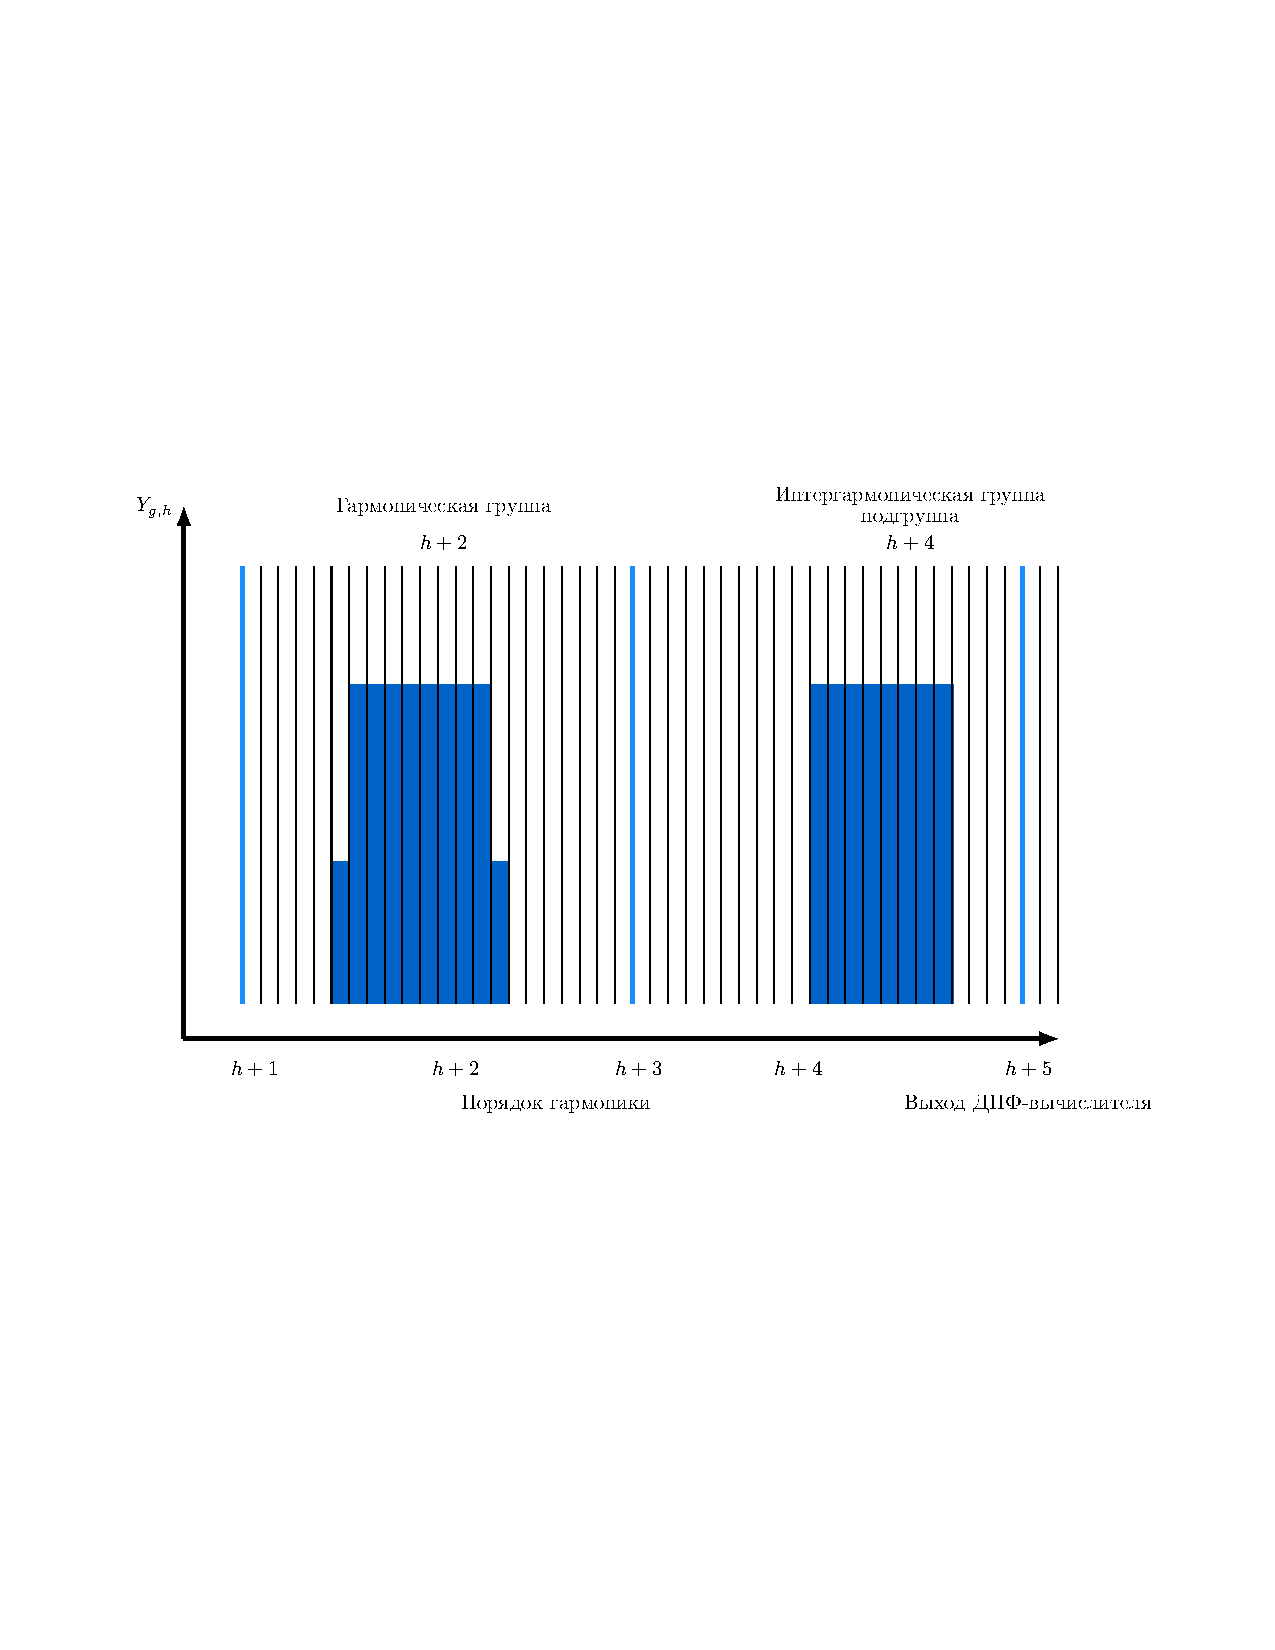
\includegraphics [scale=0.9] {scheme_of_harmonic_and_interharmonic_groups}
	\caption{Схема образования гармонических и интергармонических групп (для систем электроснабжения частотой  $50$ Гц).}
	\label{img:picture1.1}
\end{figure}


Среднеквадратичное значение гармонической подгруппы (r.~m.~s. value of a harmonic subgroup) обозначается как $Y_{sg, h}$. Но так же может быть заменено на силу тока $I$ или напряжение $U$ На рисунке \ref{img:picture1.2} представлено влияние колебаний напряжения при проведении исследований спектрального состава напряжения. $Y_{sg, h}$ -- обозначает квадратный корень из суммы квадратных значений гармонических составляющих и двух спектральных составляющих примыкаюхих к ней.

\begin{figure}[ht]
	\centering
	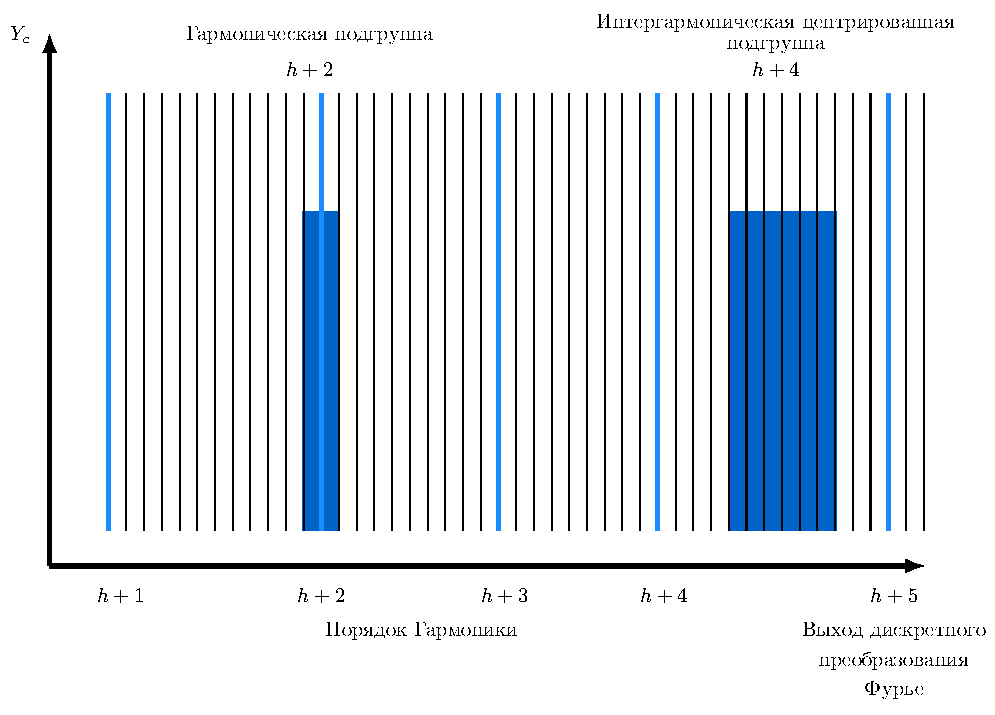
\includegraphics [scale=0.9] {process_of_harmonic_and_interharmonic_groups}
	\caption{Схема образования гармонических подгрупп и интергармонических центрированных подгрупп (для систем электроснабжения частотой  $50$ Гц).}
	\label{img:picture1.2}
\end{figure}
.


Примерами регулярно колеблющихся нагрузок, которые вызывают синусоидальные и квадратно-модулированные сигналы, являются сварочные аппараты, лазерные принтеры и приборы с интегральным контролем цикла. Для таких нагрузок частота, с которой изменяется нагрузка, будет определять частоты интергармоник.

Предполагая, что напряжение системы   и нагрузка имеет характеристику $R(t) = 1 - r \sin 2 \pi f_{0} t$, где $r<1$ и $f_{0}$  частота нагрузки варьируется. Тогда ток нагрузки: 

\begin{equation}
	\label{eq:equation1.8}
	i(t) = \frac{\upsilon (t)}{R (t)} = 
\end{equation} 

\begin{equation}
	\label{eq:equation1.8}
= \frac{\sin 2 \pi f t}{1 - r \sin 2 \pi f_0 t} = \sin 2 \pi f (1 + r \sin 2 \pi f_0 t + r^2 \sin^2 2 \pi f_0 t + r^3 \sin^3 2 \pi f_0 t + \dots) 	
\end{equation}	
	
Согласно \ref{eq:equation1.8}, $i(t)$  содержит компоненты интергармоник $f\pm f_{0},f\pm 2f_{0}, f\pm 3f_{0}, \cdots $ и~т.~д. Интергармоники будут представлены в текущем спектре $f_0$ асинхронно с $f$. 
Несинусоидальность напряжения, вызываемая высшими гармониками (ВГ), отрицательно влияет на работу силового электрооборудования и автоматики в системах электроснабжения. Из-за несоответствия норм коэффициента искажения синусоидальной формы кривой напряжения, возрастают потери электроэнергии. Повышается аварийность в кабельных сетях, вызывая сбой в работе систем релейной защиты, автоматики, телемеханики и связи.
Нормы показателей качества электрической энергии, относящиеся к несинусоидальности напряжений, измеряются и оцениваются с учетом влияния не только высших гармоник, но и групп близко расположенных комбинационных (интергармонических) составляющих \cite{532851}.
%Yacamini R. Power system harmonics. IV. Interharmonics //Power Engineering Journal. – 1996. – Т. 10. – №. 4. – С. 185-193.


Суммарный коэффициент гармонических составляющих (THD – total harmonic distortion) – это отношение среднеквадратичного значения суммы всех гармонических составляющих $Y_{H,h}$ до порядка $h_{max}$ к среднеквадратичному значению основной составляющей $Y_{H,1}$. 

\begin{equation}
	\label{eq:equation1.9}
THD_{Y} = \sqrt{\displaystyle\sum_{h=2}^{h_{max}}} (\frac{Y_{H,h}}{Y_{H,1}})^2
\end{equation} 
где $h_{max}=40$, если другое значение не установлено в международных стандартах, характеризующих нормы эмиссии гармоник.

Для тока используем символ $I$, для напряжения – $U$.
Частота гармоники $f_{(H,h)}$ (harmonic frequency) – это частота, кратная основной частоте системы электроснабжения.

После того как получили основную частоту $f_{(H,1)}$, то можно извлечь из частотного спектра спектральные составляющие. Чтобы получить гармоники используем частотный индекс и умножаем его на целое число:

\begin{equation}
	\label{eq:equation1.10}
	f_{H,h} = h \cdot f_{H,1}
\end{equation} 

Частота гармоники $f_{(H,h)}$ идентична частоте спектральной составляющей $f_{C,k}(k=hN)$.
где $k$ – номер спектральной составляющей, $h$  – порядок гармоники $N$ – число периодов.
Интергармоническая частота не кратная основной частоте.

\begin{table}[ht]
	\caption{Спектральные составляющие волны}%
	\label{tbl:test1_1}%
	\fontsize{14pt}{14pt}\selectfont
	\begin{longtable*}[c]{|l|l|} 
		\hline
		Соcтавляющие & Значения \\
		\hline
		Гармоника &
    	$f_{H,h}=h\cdot f_{H,1}$, где $h \in Z$, $h>0$
 \\
    	
    	Компонента постоянного тока &
    	$f_{H,h}=h\cdot f_{H,1}$, где $h = 0 $
 \\
    	
    	Интергармоника &
    	$f_{H,h}\neq h\cdot f_{H,1}$, где $h \in Z$, $h>0$  \\
    	
    	Субгармоника &
    	$f_{H,h} > 0$ и $h\cdot f_{H,h} < f_{H,1}$ \\
		\hline
	\end{longtable*}
\end{table}

\begin{figure}[ht]
	\centerfloat{
		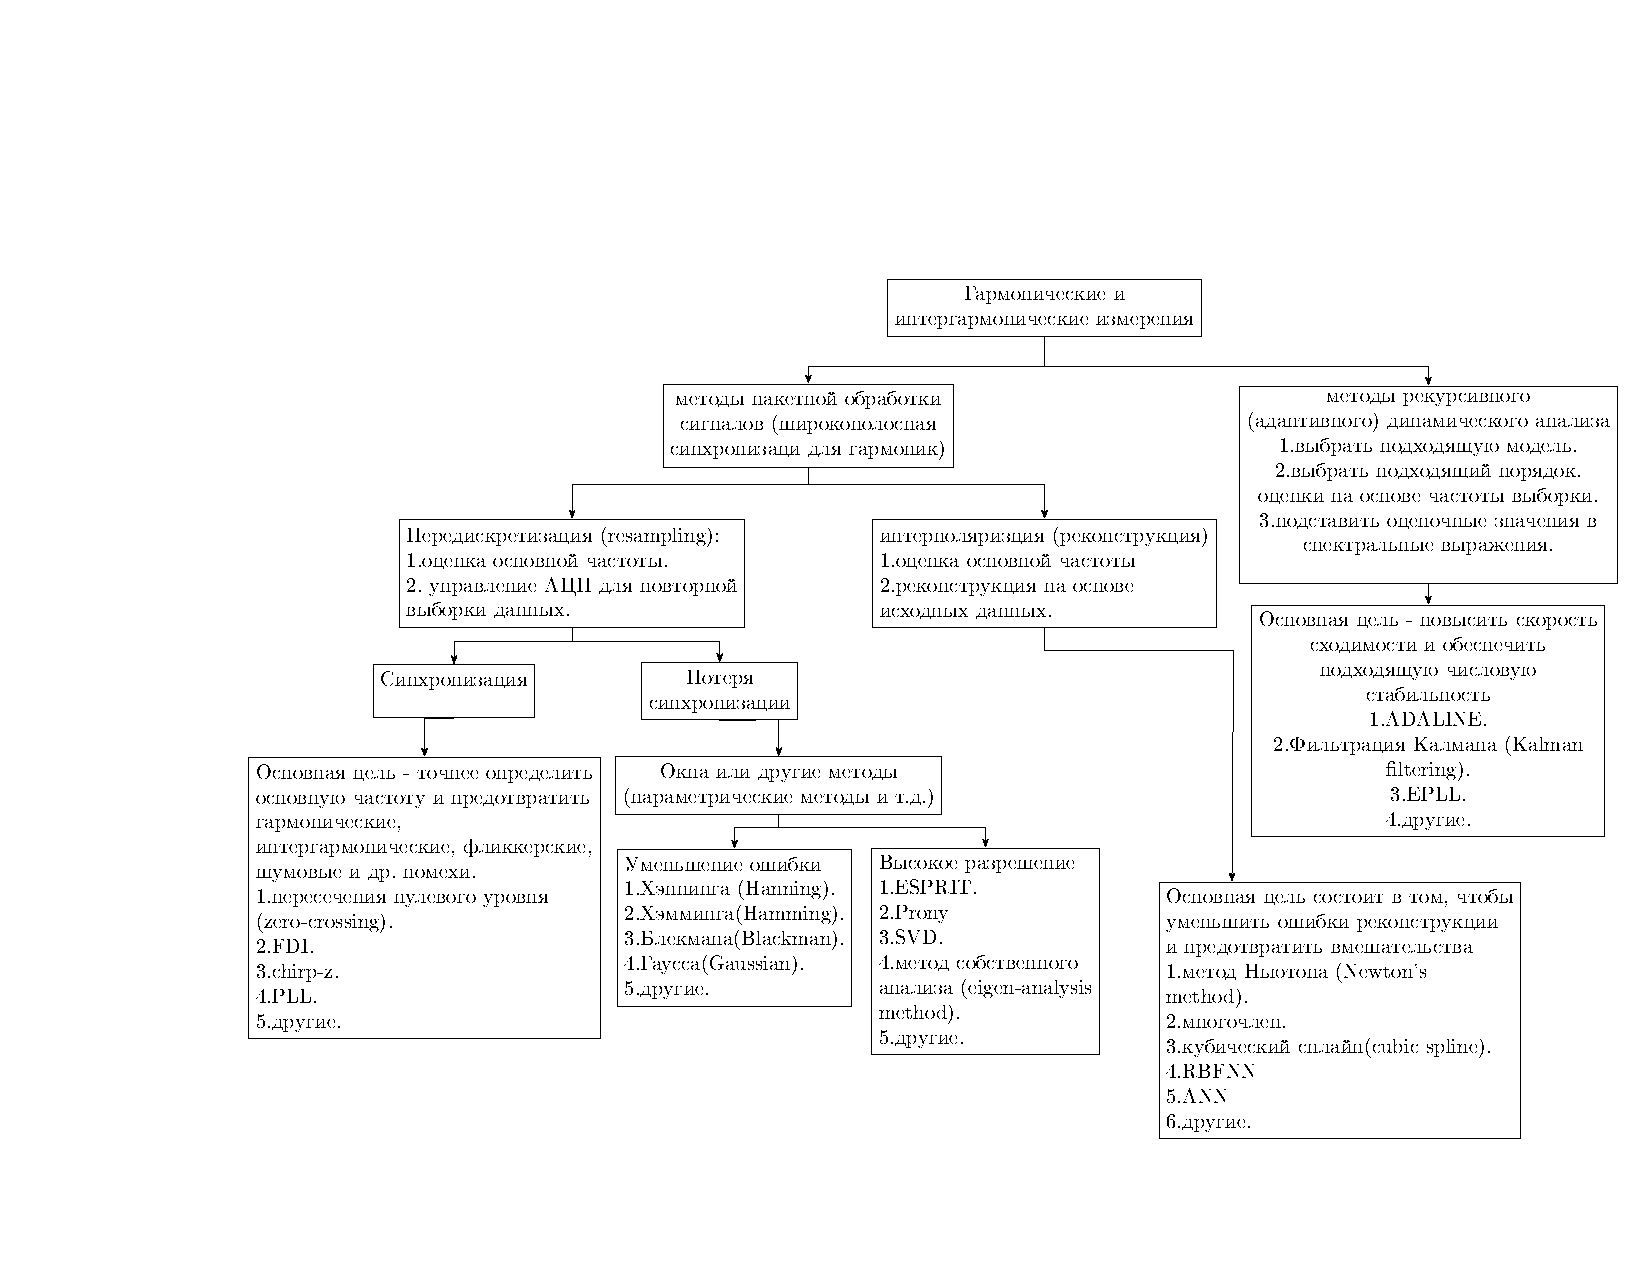
\includegraphics[scale=0.7]{picture15}
	}
	\caption{Упрощенная классификация обычно используемых методов гармонических и межгармонических оценок.}\label{fig:picture1.3}
\end{figure}

\section{Обзор обнаружения и измерения гармоник в энергосистеме} \label{sec:ch1/sec2}
% Durdhavale S. R., Ahire D. D. A review of harmonics detection and measurement in power system //International Journal of Computer Applications. – 2016. – Т. 143. – №. 10. – С. 42-45.

В любой энергосистеме крайне невозможно получить идеальный синусоидальный сигнал в каждой точке сети. Форма волны напряжения и тока значительно отличается от синусоидальной формы волны. Эти отклонения формы сигнала обычно называют гармоническим искажением \cite{durdhavale2016review}.

\begin{equation}
	\label{eq:equation1.11}
	fh = n * fundamental frequency
\end{equation} 

где $fh$ – порядок гармоник;

$n$ – целое число;

основная частота – равна $50$~Гц или $60$~Гц.

Если система имеет основную частоту $60$~Гц, то ее вторая и третьи гармоники будут иметь частоты $120$~Гц и $180$~Гц соответственно.
% 10. Harmonics Detection and Filtering [Электронный ресурс] / Life is on. – Электрон.текстовые дан. Режим доступа: https://www.se.com/ww/en/download/document/DBTP152GUI_EN/

% 12. Harmonics in your electrical system [Электронный ресурс] / EATON. – Электрон.текстовые дан. Режим доступа: https://www.newark.com/pdfs/techarticles/eaton/Eaton_Technical_Articles/UPS_Training/Powerware_Training/HarmonicsInYourElecSystem.pdf

Гармоники, которые являются не чем иным, как искаженными сигналами, имеют два типа, а именно гармоники напряжения и тока. Порядки гармоник и симметричных составляющих – это два понятия, которые обычно используются для описания гармоник. Что касается гармоник, обычно используются слова нечетные и четные гармоники, но термин тройные гармоники мало известен.

Нечетные гармоники являются характеристическими составляющими гармоник в силовой сети. Сигналы, симметричные оси времени, представлены нечетными гармониками. В случае четных гармоник они могут возникать только из сигналов, которые не симметричны оси времени \cite{soni2014review}.
% 13. Soni M. K., Soni N. Review of causes and effect of harmonics on power system //International Journal of Science, Engineering and Technology Research (IJSETR). – 2014. – Т. 3. – №. 2. – С. 214-220.
 
Представление гармонических компонентов дается с помощью уравнения:  
\begin{equation}
	\label{eq:equation1.12}
	fh = \frac{fn}{fn}\times 100
\end{equation} 

где $fh$ – текущая амплитуда гармоники n-го порядка;

$f1$ – основная амплитуда тока.

Общее гармоническое искажение (THD – Total Harmonic Distortion) широко используется при определении уровня содержания гармоник. Оно задается как отношение мощности всех гармонических составляющих к мощности основной частоты.

Обычно искаженная форма волны тока вызвана вкладом текущих порядков от $2$ до $40$. 

Значение Общего гармонического тока (THC – Total Harmonic Current) используется для установки активных фильтров:
\begin{equation}
	\label{eq:equation1.13}
	THC = \sqrt{\displaystyle\sum_{n=2}^{n=40} Ih^2}
\end{equation} 

Общий гармонический ток искажения (THDi – Total Harmonic Distortion Current) -- это значение дает общее гармоническое искажение формы волны. Это значение можно рассчитать, взяв отношение THC к основному току. Это может быть дано как:

\begin{equation}
	\label{eq:equation1.14}
	THDi = \frac{\sqrt{\displaystyle\sum_{n=2}^{n=40} Ih^2}}{I1} = \frac{THC}{I1}
\end{equation} 
где $I1$ – основной ток.

Общее гармоническое искажение напряжения (THDv – Total Harmonic Distortion of Voltage) показывает общую величину искажения в напряжении. Его можно рассчитать путем вычисления отношения гармонического напряжения к основному напряжению. Это можно записать как:

\begin{equation}
	\label{eq:equation1.15}
	THD\upsilon = \frac{\sqrt{\displaystyle\sum_{n=2}^{n=40} Vn^2}}{V1} \times 100 
\end{equation} 

где $Vn$ – амплитуда напряжения гармоники n-го порядка;

$\upsilon 1$ – основная амплитуда напряжения.

Общее искажение спроса (THD – Total Demand Distortion) - эта концепция широко используется в Северной Америке в отношении гармоник. Это отношение гармонического тока к основному току полной нагрузки. Ток полной нагрузки – это не что иное, как негармонический ток, потребляемый всеми нагрузками системы, когда система находится на пиковой нагрузке.

\begin{equation}
	\label{eq:equation1.16}
	TDD = \frac{\sqrt{\displaystyle\sum_{n=2}^{n=40} Vn^2}}{Il} = \frac{THC}{Il}
\end{equation} 

где $In$ – амплитуда тока гармоники $n$ -го порядка;

$Il$ – общий ток нагрузки, потребляемый системой.

Частичное взвешенное гармоническое искажение (PWHD – Partial Weighted Harmonic Distortion) -- это отношение тока или напряжения с выбранной группой гармоник высшего порядка от $14$ до $40$ к основному значению напряжения или тока. PWHD для тока и напряжения:

\begin{equation}
	\label{eq:equation1.17}
PWHD,I = \frac{\sqrt{\displaystyle\sum_{n=14}^{n=40} In^2}}{I1} \times 100 
\end{equation} 

\begin{equation}
	\label{eq:equation1.18}
	PWHD,V = \frac{\sqrt{\displaystyle\sum_{n=14}^{n=40} Vn^2}}{V1} 
\end{equation} 

где $I1$ – основная амплитуда тока;

$V1$ – основная амплитуда напряжения.

Гармоники влияют на силовое оборудование и компоненты \cite{soni2014review, kamenka2014six}.
% 13. Soni M. K., Soni N. Review of causes and effect of harmonics on power system //International Journal of Science, Engineering and Technology Research (IJSETR). – 2014. – Т. 3. – №. 2. – С. 214-220. 

% 14. Kamenka A. Six tough topics about harmonic distortion and Power Quality indices in electric power systems //The Schaffner Group, Luterbach. – 2014.

Гармонические искажения влияют на коэффициент мощности. Коэффициент мощности ухудшается с увеличением количества гармонических искажений. Как правило, нелинейные нагрузки приводят к плохому коэффициенту мощности.

Это оборудование рассматривается как источник гармоник. Устройства чувствительны к гармоническим искажениям. Они показывают такие эффекты, как увеличение напряжения питания, шум пересечения нуля, неисправность защитных устройств и~т.~д.

Это оборудование рассматривается как источник гармоник. Устройства чувствительны к гармоническим искажениям. Они показывают такие эффекты, как увеличение напряжения питания, шум пересечения нуля, неисправность защитных устройств и~т.~д.

Частота вызывает потери вихревых токов. Следовательно, с увеличением порядка гармоник потери на вихревые токи для трансформаторов также возрастают. В дополнение к скин-эффекту (skin effect) потери на вихревые токи при выпадении трансформатора при перегреве и сроке службы трансформатора будут уменьшены.

Конденсаторы улучшают коэффициент мощности. Они оказывают значительное влияние на гармонические уровни. При увеличении частоты гармоник емкостное сопротивление уменьшается. По мере увеличения тока увеличивается, конденсатор может перегружаться и создавать более высокое диэлектрическое напряжение.

Сбои низкого уровня в автоматических выключателях, вызванные высокой степенью тока гармонической нагрузки. Высокие значения при пересечении нуля для синусоидальной формы волны делают комплекс разрушения для искажения нагрузки. Следовательно, токи гармонической нагрузки приводят к отказам цепи.

\section{Оценка гармоник в реальном времени по мощности системы} \label{sec:ch1/sec3}
% Enayati J., Moravej Z. Real-time harmonics estimation in power systems using a novel hybrid algorithm //IET Generation, Transmission & Distribution. – 2017. – Т. 11. – №. 14. – С. 3532-3538.

Наличие искажений формы напряжения и тока обычно выражается через гармонические частоты, которые являются целыми кратными сгенерированной частоты \cite{arrillaga1997power, rodriguez2017novel}. 
% 1. Arrillaga J. et al. Power system harmonic analysis. – John Wiley & Sons, 1997.
% 2. Rodriguez-Guerrero M. A. et al. A novel methodology for modeling waveforms for power quality disturbance analysis //Electric Power Systems Research. – 2017. – Т. 143. – С. 14-24.
Применение синусоидального напряжения к электронным нагрузкам приводит к несинусоидальным падениям тока. Протекание этого тока через импеданс линий электропередач вызывает искажения напряжения на клеммах нагрузки. Кроме того, насыщение трансформаторов вызывает повышенное искажение тока/напряжения. Это представляет собой важную проблему качества электроэнергии, которая оказывает вредное воздействие на оборудование энергосистемы. Следовательно, уровни гармоник должны поддерживаться в стандартной точке с использованием разработанных фильтров, применяемых в источнике гармоник для предотвращения распространения гармоник. Предварительным этапом фильтрации нежелательных частот является вывод параметров гармоник.
Были проведены значительные исследования в области оценки гармоник с целью определения амплитуды и фазы гармоник в шумо-искаженном сигнале. В \cite{chen2013comparative} авторы представляют краткий обзор различных методов и их проблем в оценке гармоник.
% 3. Chen C. I., Chen Y. C. Comparative study of harmonic and interharmonic estimation methods for stationary and time-varying signals //IEEE Transactions on Industrial Electronics. – 2013. – Т. 61. – №. 1. – С. 397-404.
ДПФ в его различных формах является наиболее распространенным методом частотной области для анализа формы волны \cite{guo2016method, 6919330, 7172520, beltran2017fast}. 
% 4. Guo X. et al. Method for radial vibration modelling in switched reluctance motor //IET Electric Power Applications. – 2016. – Т. 10. – №. 9. – С. 834-842.

% 5. H. Wen, J. Zhang, Z. Meng, S. Guo, F. Li and Y. Yang, "Harmonic Estimation Using Symmetrical Interpolation FFT Based on Triangular Self-Convolution Window," in IEEE Transactions on Industrial Informatics, vol. 11, no. 1, pp. 16-26, Feb. 2015, doi: 10.1109/TII.2014.2362491.

% 6. M. S. Reza and V. G. Agelidis, "A Robust Technique for Single-Phase Grid Voltage Fundamental and Harmonic Parameter Estimation," in IEEE Transactions on Instrumentation and Measurement, vol. 64, no. 12, pp. 3262-3273, Dec. 2015, doi: 10.1109/TIM.2015.2444259.

% 7. Beltran-Carbajal F., Silva-Navarro G. A fast parametric estimation approach of signals with multiple frequency harmonics //Electric Power Systems Research. – 2017. – Т. 144. – С. 157-162.

Этот периодический метод имеет три основных проблемных момента: алиасинг (aliasing), утечка (leakage) и пикет (picket-fence) \cite{4102347}.
% 8. A. A. Girgis and F. M. Ham, "A Quantitative Study of Pitfalls in the FFT," in IEEE Transactions on Aerospace and Electronic Systems, vol. AES-16, no. 4, pp. 434-439, July 1980, doi: 10.1109/TAES.1980.308971.
Теоретически методы, основанные на ДПФ, точны при анализе периодических и стационарных сигналов, в которых частотные составляющие кратны разрешающей способности по частоте окна выборки. Однако основная частота энергосистемы имеет отклонения от номинального значения, что приводит к снижению точности ДПФ. Среди методов во временной области, применяемых к оценке гармоник, часто используется метод линейного фильтра Калмана (KF -- Kalman filter) \cite{dash1998fast}. 
% 9. Dash P. K. et al. Fast tracking of transient power system signals using fuzzy LMS algorithm //International Journal of Electrical Power & Energy Systems. – 1998. – Т. 20. – №. 8. – С. 555-561.
Задача оценки параметров гармоники (то есть амплитуды и фазы гармоник) является нелинейной задачей. Затем, в большом количестве гармоник, отслеживание фаз синусоид выходит за пределы возможностей линейного KF, особенно в присутствии интенсивного шума. В некоторых источниках вводятся адаптивные методы с переменным коэффициентом усиления, чтобы справиться с нелинейным характером проблемы \cite{1413428, ray2012ensemble, dash1996harmonic, singh2016several}.
% 10. K. K. C. Yu, N. R. Watson and J. Arrillaga, "An adaptive Kalman filter for dynamic harmonic state estimation and harmonic injection tracking," in IEEE Transactions on Power Delivery, vol. 20, no. 2, pp. 1577-1584, April 2005, doi: 10.1109/TPWRD.2004.838643.

% 11. P. K. Ray and B. Subudhi, "Ensemble-Kalman-Filter-Based Power System Harmonic Estimation," in IEEE Transactions on Instrumentation and Measurement, vol. 61, no. 12, pp. 3216-3224, Dec. 2012, doi: 10.1109/TIM.2012.2205515.

% 12. Dash P. K. et al. Harmonic estimation in a power system using adaptive perceptrons //IEE Proceedings-Generation, Transmission and Distribution. – 1996. – Т. 143. – №. 6. – С. 565-574.

% 13. Singh S. K. et al. Several variants of Kalman Filter algorithm for power system harmonic estimation //International Journal of Electrical Power & Energy Systems. – 2016. – Т. 78. – С. 793-800.

Методы адаптивной оценки чувствительны к настройке адаптивных факторов и скорости их изменения. Например, адаптивный KF требует точной настройки четырех свободных параметров, а также требует априорного знания шума \cite{ray2012ensemble}. Гармоники нелинейно связаны с выделенной фазой, что создает дополнительные препятствия для точного прогнозирования параметров гармоник.
Следовательно, искусственные нейронные сети (ИНС, ANNs-- artificial neural networks) применяются для получения нелинейных характеристик задачи \cite{6553247, 4084681, lin2016electromagnetic, joorabian2009harmonic}. 
% 14. M. Valtierra-Rodriguez, R. de Jesus Romero-Troncoso, R. A. Osornio-Rios and A. Garcia-Perez, "Detection and Classification of Single and Combined Power Quality Disturbances Using Neural Networks," in IEEE Transactions on Industrial Electronics, vol. 61, no. 5, pp. 2473-2482, May 2014, doi: 10.1109/TIE.2013.2272276.

% 15. H. C. Lin, "Intelligent Neural Network-Based Fast Power System Harmonic Detection," in IEEE Transactions on Industrial Electronics, vol. 54, no. 1, pp. 43-52, Feb. 2007, doi: 10.1109/TIE.2006.888685.

% 16. Lin F., Zuo S., Wu X. Electromagnetic vibration and noise analysis of permanent magnet synchronous motor with different slot-pole combinations //IET Electric Power Applications. – 2016. – Т. 10. – №. 9. – С. 900-908.

% 17. Joorabian M., Mortazavi S. S., Khayyami A. A. Harmonic estimation in a power system using a novel hybrid Least Squares-Adaline algorithm //Electric power systems research. – 2009. – Т. 79. – №. 1. – С. 107-116.
Несмотря на простоту реализации, если параметры ИНС не установлены должным образом, процесс оценки ИНС будет ошибочный, что приведет к снижению точности результатов оценки \cite{moravej2014hybrid}. 
% 18. Moravej Z., Enayati J. A hybrid least squares–clonal selection based algorithm for harmonics estimation //International Transactions on Electrical Energy Systems. – 2014. – Т. 24. – №. 1. – С. 1-15.
Алгоритмы стохастической оптимизации основаны на стохастическом поиске оптимального решения данной задачи. Эти методы неоднократно используются для оценки гармоник в качестве другой альтернативы \cite{1193852, 4469961, singh2016power}. 
% 19. M. Bettayeb and Uvais Qidwai, "A hybrid least squares-GA-based algorithm for harmonic estimation," in IEEE Transactions on Power Delivery, vol. 18, no. 2, pp. 377-382, April 2003, doi: 10.1109/TPWRD.2002.807458.

% 20. Z. Lu, T. Y. Ji, W. H. Tang and Q. H. Wu, "Optimal Harmonic Estimation Using A Particle Swarm Optimizer," in IEEE Transactions on Power Delivery, vol. 23, no. 2, pp. 1166-1174, April 2008, doi: 10.1109/TPWRD.2008.917656.

% 21. Singh S. K. et al. Power system harmonic estimation using biogeography hybridized recursive least square algorithm //International Journal of Electrical Power & Energy Systems. – 2016. – Т. 83. – С. 219-228.
Однако прямое применение алгоритмов стохастической оптимизации к практическим задачам крайне ограничено. Следующее объясняет причины ограниченной возможности стохастических алгоритмов в оценке гармоник:
\begin{itemize}
\item Поскольку амплитуды и фазы гармоник количественно различаются при разных масштабах, единицах и физической интерпретации, окончательное решение трудно получить \cite{4469961}.

\item Стохастические методы испытывают трудности в тонкой настройке локального поиска; они проводят большую часть времени, соревнуясь между разными холмами, а не улучшая решение вдоль одного холма, на котором расположена оптимальная точка \cite{singh2016power}. Реальные модели сигналов энергосистемы являются нелинейными по фазе и линейными по амплитуде \cite{dash1998fast, singh2016several, 1413428, ray2012ensemble, dash1996harmonic, singh2016several}. Рассмотрение оценки гармоник как полностью нелинейной задачи снижает скорость сходимости алгоритма. Поэтому гибридные алгоритмы применяются для решения задачи оценки гармоник как отдельных задач оценки амплитуды и фазы \cite{joorabian2009harmonic, moravej2014hybrid, 1193852, 4469961, singh2016power, 6202692б, 6419813, nanda2016new}. Поскольку сигналы энергосистемы являются динамическими, было обнаружено, что некоторые недавние адаптивные методы \cite{6522142, 6908042} подходят для разложения многокомпонентных статических и динамических сигналов. Однако из-за использования базового быстрого преобразования Фурье точность разложения ближайших частотных компонентов может быть немного ниже.
\end{itemize}
% 21. Singh S. K. et al. Power system harmonic estimation using biogeography hybridized recursive least square algorithm //International Journal of Electrical Power & Energy Systems. – 2016. – Т. 83. – С. 219-228.
%%%%%%
% 9. Dash P. K. et al. Fast tracking of transient power system signals using fuzzy LMS algorithm //International Journal of Electrical Power & Energy Systems. – 1998. – Т. 20. – №. 8. – С. 555-561.

% 10. K. K. C. Yu, N. R. Watson and J. Arrillaga, "An adaptive Kalman filter for dynamic harmonic state estimation and harmonic injection tracking," in IEEE Transactions on Power Delivery, vol. 20, no. 2, pp. 1577-1584, April 2005, doi: 10.1109/TPWRD.2004.838643.

% 11. P. K. Ray and B. Subudhi, "Ensemble-Kalman-Filter-Based Power System Harmonic Estimation," in IEEE Transactions on Instrumentation and Measurement, vol. 61, no. 12, pp. 3216-3224, Dec. 2012, doi: 10.1109/TIM.2012.2205515.

% 12. Dash P. K. et al. Harmonic estimation in a power system using adaptive perceptrons //IEE Proceedings-Generation, Transmission and Distribution. – 1996. – Т. 143. – №. 6. – С. 565-574.

% 13. Singh S. K. et al. Several variants of Kalman Filter algorithm for power system harmonic estimation //International Journal of Electrical Power & Energy Systems. – 2016. – Т. 78. – С. 793-800.
%%%%%
% 17. Joorabian M., Mortazavi S. S., Khayyami A. A. Harmonic estimation in a power system using a novel hybrid Least Squares-Adaline algorithm //Electric power systems research. – 2009. – Т. 79. – №. 1. – С. 107-116.

% 18. Moravej Z., Enayati J. A hybrid least squares–clonal selection based algorithm for harmonics estimation //International Transactions on Electrical Energy Systems. – 2014. – Т. 24. – №. 1. – С. 1-15.

% 19. M. Bettayeb and Uvais Qidwai, "A hybrid least squares-GA-based algorithm for harmonic estimation," in IEEE Transactions on Power Delivery, vol. 18, no. 2, pp. 377-382, April 2003, doi: 10.1109/TPWRD.2002.807458.

% 20. Z. Lu, T. Y. Ji, W. H. Tang and Q. H. Wu, "Optimal Harmonic Estimation Using A Particle Swarm Optimizer," in IEEE Transactions on Power Delivery, vol. 23, no. 2, pp. 1166-1174, April 2008, doi: 10.1109/TPWRD.2008.917656.

% 21. Singh S. K. et al. Power system harmonic estimation using biogeography hybridized recursive least square algorithm //International Journal of Electrical Power & Energy Systems. – 2016. – Т. 83. – С. 219-228.

% 22. S. K. Jain, S. N. Singh and J. G. Singh, "An Adaptive Time-Efficient Technique for Harmonic Estimation of Nonstationary Signals," in IEEE Transactions on Industrial Electronics, vol. 60, no. 8, pp. 3295-3303, Aug. 2013, doi: 10.1109/TIE.2012.2200218.

% 23. S. K. Jain and S. N. Singh, "Low-Order Dominant Harmonic Estimation Using Adaptive Wavelet Neural Network," in IEEE Transactions on Industrial Electronics, vol. 61, no. 1, pp. 428-435, Jan. 2014, doi: 10.1109/TIE.2013.2242414.

% 24. Nanda S., Chakravorty T., Dash P. K. A new Taylor-LMS adaptive filter for parameter estimation of power signals including distributed generation systems //Australian Journal of Electrical and Electronics Engineering. – 2016. – Т. 13. – №. 3. – С. 174-194.
%%%%%%%
% 25. J. Gilles, "Empirical Wavelet Transform," in IEEE Transactions on Signal Processing, vol. 61, no. 16, pp. 3999-4010, Aug.15, 2013, doi: 10.1109/TSP.2013.2265222.

% 26. K. Thirumala, A. C. Umarikar and T. Jain, "Estimation of Single-Phase and Three-Phase Power-Quality Indices Using Empirical Wavelet Transform," in IEEE Transactions on Power Delivery, vol. 30, no. 1, pp. 445-454, Feb. 2015, doi: 10.1109/TPWRD.2014.2355296.

В статье \cite{enayati2017real} для оценки фаз гармоник применяется алгоритм, основанный на фильтре Калмана, наряду с линейной оценкой на основе наименьших квадратов для оценки амплитуд. Повторный расширенный фильтр Калмана (IEKF -- iterated extended Kalman filter) применяется для решения нелинейных уравнений, которые описывают взаимосвязь фаз и исходной формы волны. Оценки амплитуд методом наименьших квадратов (LS -- least squares) рекурсивно вычисляются с использованием метода рекурсивных методов наименьших квадратов (RLS -- recursive least squares). Этот гибридный алгоритм оценивает амплитуды и фазы отдельно. Следовательно, различные масштабы, единицы и физические интерпретации исследуются отдельными алгоритмами, что приводит к меньшему количеству итераций, чтобы сходиться. 
% Enayati J., Moravej Z. Real-time harmonics estimation in power systems using a novel hybrid algorithm //IET Generation, Transmission & Distribution. – 2017. – Т. 11. – №. 14. – С. 3532-3538.

Из-за наличия искажений в электрических формах волны, формы волны тока/напряжения обычно выражаются как периодические функции, частоты которых кратны сгенерированной частоте. Дискретная форма времени функции может быть записана как \cite{moravej2014hybrid, 1193852, 4469961}.
% 18. Moravej Z., Enayati J. A hybrid least squares–clonal selection based algorithm for harmonics estimation //International Transactions on Electrical Energy Systems. – 2014. – Т. 24. – №. 1. – С. 1-15.

% 19. M. Bettayeb and Uvais Qidwai, "A hybrid least squares-GA-based algorithm for harmonic estimation," in IEEE Transactions on Power Delivery, vol. 18, no. 2, pp. 377-382, April 2003, doi: 10.1109/TPWRD.2002.807458.

% 20. Z. Lu, T. Y. Ji, W. H. Tang and Q. H. Wu, "Optimal Harmonic Estimation Using A Particle Swarm Optimizer," in IEEE Transactions on Power Delivery, vol. 23, no. 2, pp. 1166-1174, April 2008, doi: 10.1109/TPWRD.2008.917656.
\begin{equation}
\label{eq:equation1.19}
	Z_k = {\sum_{n=1}^{N} A_n \sin({2 \pi  f n  k  \tau_{s} + \theta_n}) + \sigma_v  randn(k)}
\end{equation}
где $n = 1, 2,\cdots, N$ представляет порядок гармоники; $A_n$, $\theta_n$ и $f$ -- амплитуда, фазовый угол и основная частота, $\sigma_v randn(k)$ аддитивный гауссов шум, а $\tau_s$ период дискретизации. Состояния, которые следует оценить как $A_n$, $\theta_n$.

Как видно в статье \cite{enayati2017real}, полученная модель нелинейна по фазе синусоид, что приводит к дальнейшим препятствиям для точной оценки целевых состояний. Однако применение линейных алгоритмов для оценки амплитуды повышает скорость сходимости алгоритма. Следовательно, идея использования гибридных алгоритмов в качестве простых и гибких подходов стала популярной для получения гармонических параметров.

Алгоритм оценки амплитуды, применяемый в \cite{enayati2017real} статье, основан на критерии наименьших квадратов. В этом разделе описывается рекурсивный метод для вычисления наименьших квадратов оценки амплитуд. В целом, линейная рекурсивная оценка может быть записана следующим образом:
\begin{equation}
\label{eq:equation1.20}	
	Y_{k}=H_{k}x+v_{k}
\end{equation}

\begin{equation}
\label{eq:equation1.21}
	\widehat{x} = \widehat{x}_{k-1}+K_{k}(Y_{k} -H_{k} \widehat{x}_{k-1})
\end{equation}

где вектор состояния $\widehat{x}_{k}$ оценивается на основе предыдущей оценки $\widehat{x}_{k-1}$ и нового измерения $Y_{k}$.$ H_{k}$ и $ v_{k}$ - матрица усиления и шум измерения, соответственно. Учитывая амплитуды как вектор состояния $x$, структурная матрица $H_{k}$ будет иметь вид
\begin{equation}
\label{eq:equation1.22}
	H_{k}= [sin(2\pi f k\tau_{s}  + \theta_{1}) ...sin(2\pi f nk\tau_{s}+ \theta n)]
\end{equation}

где $\theta$ оценивается с использованием повторного расширенного фильтра Калмана. Рекурсивное уравнение для ковариации ошибки оценки метода наименьших квадратов можно записать в виде:
\begin{equation}
\label{eq:equation1.23}
	P_{k} =(1+\alpha)[P_{k-1}^{-1}+H_{k}^{T} R_{k-1}^{-1} H_{k}]^{-1}
\end{equation}

где $\alpha$ - настраивающий фактор, контролирующий влияние измерения по оценке и R - ковариационная матрица измерения шума. Чтобы найти значение $K_{k}$, используются следующие формулы:
\begin{equation}
\label{eq:equation1.24}
	K_{k} = P_{k} H_{k}^{T} H_{k}^{-1}
\end{equation}

Пакетные алгоритмы, такие как метод наименьших квадратов, дополняют структурную матрицу $H$ при получении нового измерения. Тогда вычислительные усилия метода наименьших квадратов быстро перерастут ресурсы. Между тем, рекурсивные алгоритмы, такие как рекурсивные методы наименьших квадратов, не нуждаются в каком-либо увеличении матрицы \cite{6574296, bettayeb1998recursive}. Это свойство рекурсивных алгоритмов позволяет использовать рекурсивные методы наименьших квадратов для онлайн-реализации и дает оценки с возможностью отслеживания во времени \cite{bettayeb1998recursive}.
% 27. C. Rakpenthai, S. Uatrongjit, N. R. Watson and S. Premrudeepreechacharn, "On Harmonic State Estimation of Power System With Uncertain Network Parameters," in IEEE Transactions on Power Systems, vol. 28, no. 4, pp. 4829-4838, Nov. 2013, doi: 10.1109/TPWRS.2013.2273943.
% 28. Bettayeb M., Qidwai U. Recursive estimation of power system harmonics //Electric power systems research. – 1998. – Т. 47. – №. 2. – С. 143-152.

Фильтр  в его различных формах четко установлен в качестве основного инструмента для анализа и решения широкого класса задач оценки \cite{simon2006optimal}. В этом разделе уравнения повторного расширенного фильтра Калмана разработаны с использованием представления переменной состояния искаженного сигнала. Состояния для оценки определяются как:
% 29. Simon D. Optimal state estimation: Kalman, H infinity, and nonlinear approaches. – John Wiley & Sons, 2006.
\begin{equation}
\label{eq:equation1.25}	
	\textbf{X} = [\theta_{1}, \theta_{2},..., \theta_{n}]
\end{equation}

Уравнение дискретного времени системы, описывающей динамику состояний, имеет следующий вид:
\begin{equation}
\label{eq:equation1.26}	
	X_{k+1,k} = \varphi (t_{k},t_{k+1}) X_{k,k}+ w_{k+1}
\end{equation}

где матрица перехода $\varphi$ $(t_{k}$, $t_{k + 1})$ является $(n + 1 \times n + 1)$ единичной матрицей, а $w$ является шумом процесса. Основываясь на наших знаниях о динамике системы, состояния в повторном расширенном фильтре Калмана обновляются с использованием обновления времени (7). Для вычисления уравнения обновления времени ковариационной матрицы применяется следующая формулировка:
\begin{equation}
\label{eq:equation1.27}	
	P_{k+1,k} = \varphi (t_{k},t_{k+1}) P_{k,k} \varphi (t_{k},t_{k+1})^{T}
\end{equation}

Согласно \ref{eq:equation1.19}, величина тока/напряжения в каждый момент $(Z_{k})$ доступна для измерения. Это измерение искажено последовательностью чисто гауссовского шума с нулевым средним и дисперсией $ \sigma_{v}^{2}.$

Каждый раз, когда получено измерение, вектор состояния и ковариационная матрица должна быть обновлена. Нелинейный процесс в \ref{eq:equation1.19} можно выразить через состояния повторного расширенного фильтра Калмана
\begin{equation}
\label{eq:equation1.28}		
	Z_{k+1}=h(X_{k + 1,k}) + \sigma_v randn(k)
\end{equation}

Тогда матрица коэффициентов усиления вычисляется следующим образом:
\begin{equation}
	\label{eq:equation1.29}		
G_{k+1} = P_{k+1,k} \frac{{\partial h}^T}{\partial \textbf{X}} {\left( {\frac{\partial h}{\partial \textbf{X}} P_{k+1,k} \frac{{\partial h}^T}{\partial \textbf{X}} + \sigma_v^2 }\right) }^{-1}
\end{equation}

Уравнения обновления результатов измерений для вектора состояния и ковариационной матрицы строятся с использованием \ref{eq:equation1.30} и (12) соответственно.

\begin{equation}
\label{eq:equation1.30}		
X_{k+1,k+1} = X_{k+1,k} + G_{k+1}[Z_{k+1}-h(X_{k+1,k})]	
\end{equation}

\begin{equation}
	\label{eq:equation1.31}		
	P_{k+1,k+1} = \left[ {I - G_{k+1} + \frac{\partial h}{\partial \textbf{X}}} \right] P_{k+1,k}
\end{equation}

$X_{k + 1, k + 1}$ - лучшая оценка для вектора состояния $X$ по сравнению с $X_{k + 1, k}$, потому что этот вектор использует информацию измерений. Следовательно, восстановление линеаризованной матрицы измерений $\frac{\partial h}{\partial \textbf{X}}$ вокруг
новая оценка $X_{k + 1, k + 1}$ уменьшает ошибку линеаризации. Уравнения обновления измерений можно пересчитать с использованием новых матриц измерения и усиления. Этот процесс приводит к лучшей оценке $X_{k + 1, k + 1}$. Повторную линеаризацию измерительной матрицы можно повторять столько раз.
сколько угодно раз, хотя для большинства проблем большинство возможное улучшение достигается только линеаризацией один раз \cite{simon2006optimal}. 
% 29. Simon D. Optimal state estimation: Kalman, H infinity, and nonlinear approaches. – John Wiley & Sons, 2006.

\begin{equation}
	\label{eq:equation1.32}		
	P_{k+1,k} = P_{k+1,k+1}
\end{equation}

\begin{equation}
	\label{eq:equation1.33}		
	X_{k+1,k} = X_{k+1,k+1}
\end{equation}

\begin{equation}
	\label{eq:equation1.34}		
	G_{k+1} = P_{k+1,k} \frac{{\partial h}^T}{\partial \textbf{X}} {\left( {\frac{\partial h}{\partial \textbf{X}}P_{k+1,k}\frac{{\partial h}^T}{\partial \textbf{X}} + \sigma_v^2} \right) }^{-1}
\end{equation}

\begin{equation}
\label{eq:equation1.35}		
X_{k+1,k+1} = X_{k+1,k} + G_{k+1} \left[ {Z_{k+1} - h(X_{k+1,k})} \right]	
\end{equation}

\begin{equation}
	\label{eq:equation1.36}		
	P_{k+1,k+1} = \left[ {I - G_{k+1}  } \right]	\frac{\partial h}{\partial \textbf{X}} P_{k+1,k}
\end{equation}

На каждой итерации гибридный алгоритм применяет повторяющиеся расширенния
алгоритма фильтра Калмана для фазы предварительного расчета. Далее оценочные состояния повторных расширенных алгоритмов фильтра Калмана вставлены в структурную матрицу рекурсивных наименьших квадратов для оценки амплитуд гармоник. Процесс повторяется до тех пор, пока не будет достигнута приемлемая сходимость. \textbf{На рис. 1} представлена блок-схема для формулировки рекурсивного метода наименьших квадратов и повторного расширенного Алгоритм фильтра Калмана.

% закончить рисунок
\begin{figure}[ht]
	\centering
	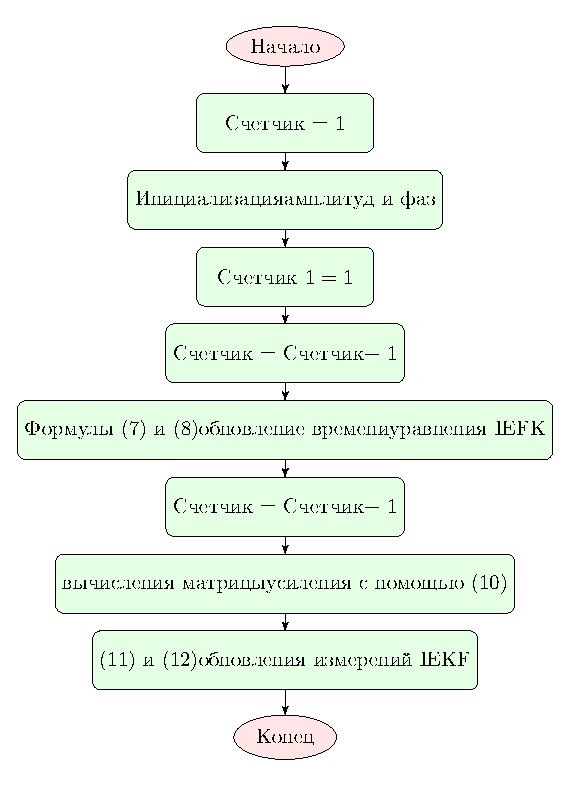
\includegraphics [scale=0.9] {Filter_Kalmana.pdf}
	\caption{Последовательность операций в алгоритме RLS – IEKF.}
	\label{img:picture1.3}
\end{figure}

\section{Улчшенный алгоритм частоты путем развертывания фазы методом наименьших квадратов} \label{sec:ch1/sec4}

Оценка частоты сложной синусоиды является фундаментальной проблемой в обработке сигналов и находит применение во многих областях. Общая модель сигнала:
\begin{equation}
	\label{eq:equation1.41}	
	y(n)=Ae^{j2 \pi(\theta+fn)}+ \omega(n) 
\end{equation}

где частота $f$, фаза $\theta$ и амплитуда A являются детерминированными, но неизвестными константами, а N - количество выборок. $\omega(n) = \omega_I(n) + j\omega_Q(n)$ - это комплексный белый гауссовский шум с нулевым средним и дисперсией $2\sigma^2 \times \omega_I (n)$ и $\omega_Q(n)$ независимы и нормально распределены с нулевым средним и дисперсией $\sigma^2 \times f$ и $ \theta$ находятся в $[- 1 / 2,1 / 2)$. Проблема состоит в оценке $f$.

Хорошо известно, что классическая оценка периодограммы [8] считается наиболее эффективной. Однако реализация этой модели очень сложна. Треттер [10] доказал, что фазовый шум приблизительно представляет собой белый гауссовский шум, и фаза может быть развернута. Затем, используя развернутую фазу, $f$ и $\theta$ можно оценить с помощью линейной регрессии. Одна общая оценка развертки фазы была впервые предложена Каем [4], и, вычисляя первые разности аргументов $y(n)$, оценка параметра может рассматриваться как линейная задача. Этот вид модели имеет простую структуру и хорошо работает при высоком Отношении Сигнал / Шум (SNR). Однако он плохо работает при низком SNR . По сравнению с другими моделями развертки фазы, модель развертки фазы наименьших квадратов (LSPUE) имеет гораздо лучшую производительность при низком SNR , что было изучено другими исследователями [6,12].

В этой статье мы предлагаем Улучшенную Оценку Развертки Фазы Методом Наименьших Квадратов (ILSPUE). ILSPUE выполняет
развертывание фазы по методу наименьших квадратов на основе новой фазовой модели. Поскольку новая фазовая модель более точна, чем предыдущая модель, ILSPUE  имеет лучшую производительность, что будет показано ниже. Основной вклад этой статьи состоит в том, что мы вводим оптимальную линейную фазовую модель для развертывания фазы методом наименьших квадратов, выводим новую целевую функцию и и демонстрируем, что новая целевая функция более точна. Затем, на основе новой целевой функции, мы представляем ILSPUE , и производительность LSPUE  улучшается.

Аргумент $y(n)$, обозначенный $\angle y(n)$, имеет вид:

\begin{equation}
\label{eq:equation1.42}	
	\angle y(n)=2 \pi(\theta+fn+u_n)(mod2 \pi)
\end{equation}

где $u_n$ - фазовый шум. Пусть $Y_n = y(n)/2 \pi$ , тогда:

\begin{equation}
\label{eq:equation1.43}	
	Y_n =<\theta+fn+u_n>
\end{equation}

где $<x> = x - [x]$- дробная часть $x$, а $[x]$ обозначает ближайшее к $x$ целое число. Формулу (3) можно записать как:

\begin{equation}
\label{eq:equation1.44}	
	Y_n= \theta+fn+u_n-k_n
\end{equation}

где $kn =[\theta + fn + un]$. Для LSPUE в [6,12] фазовая модель (4) основана на модели из [10], а фазовый шум $u_n$ аппроксимируется как: $u_n= \omega_Q(n)/(2 \pi A)$

Поскольку $\omega_Q(n)$ - это белый гауссовский шум, а $A$ - константа, согласно (4) функция суммы квадратов (SSF) равна:

\begin{equation}
\label{eq:equation1.45}		
	\sum_{n=0}^{N-1} (Y_n- \theta -fn +k_n)^2
\end{equation}

LSPUE  должен найти оптимальные $f$ и $\theta$, минимизирующие (5).

Усовершенствованная фазовая модель была дана в [1], которая оказалась более точной, чем модель в [10]. Используя эту фазовую модель для (4), $u_n$ аппроксимируется как $u_n = \omega_Q(n)/(2 \pi \sqrt{Arn})$, где $rn = | y (n) |$ - абсолютное значение $y(n)$. Учитывая, что $r_n$ является переменной, согласно (4) Улучшенная Функция Суммы Квадратов (ISSF) задается как:

\begin{equation}
\label{eq:equation1.46}	
	S(f, \theta, k_n) = \sum_{n=0}^{N-1} r_n (Y_n- \theta -fn +k_n)^2
\end{equation}

Аналогично, ILSPUE должен найти оптимальные $f$ и $\theta$, минимизирующие $S (f, \theta, kn)$. На основе улучшенной линейно-фазовой модели ISSF (6) является более точным и может быть получен лучший результат оценки.

Теперь мы продемонстрируем, что целевая функция (Формула №6) более точна, чем функция (Формула №5) напрямую. Учитывая, что $y(n) = r_ne^{ j2\pi (Y_n + k_n)}$, согласно (1) SSF равна $J(f, \theta, k_n)$ и является:

$$
J (f, \theta, k_n) = \sum_{n=0}^{N-1} (r_n \cos(2 \pi (Y_n+k_n)) -A\cos(2 \pi(\theta+fn)))^2
$$

\begin{equation}
\label{eq:equation1.47}		
	+(r_n \sin(2\pi(Y_n+k_n))-A\sin(2\pi(\theta+fn)))^2 
\end{equation}

$$ = \sum_{n=0}^{N-1} r_n^2+A^2-2Ar_n\cos(2\pi(Y_n-\theta-fn+k_n))$$

$$ \infty \sum_{n=0}^{N-1} -Ar_n\cos(2\pi(Y_n-\theta-fn+k_n))$$

В условиях комплексного белого гауссовского шума $\omega (n), J(f, \theta, k_n) = \sum_{n=0}^{N-1}-Ar_n\cos(2\pi$
$(Y_n-\theta-fn+k_n))$ 
является точной целевой функцией без какого-либо приближения. Поскольку $J(f, \theta, k_n)$ соответствует нелинейной модели, мы должны приближенно обозначать. Применяя разложение Тейлора второго порядка к $J(f, \theta, k_n)$, получаем:

$$
J(f, \theta, k_n) \approx \sum_{n=0}^{N-1} -Ar_n+2\pi^2Ar_n(Y_n-\theta-fn+k_n)^2
$$

\begin{equation}
\label{eq:equation1.48}	
	\infty \sum_{n=0}^{N-1} r_n (Y_N-\theta-FN+K_N)^2
\end{equation}
$$
=S(f,\theta,k_n)
$$


Следовательно, $S (f, \theta, k_n)$ - это приближение второго порядка для $J (f, \theta, k_n)$. В то время как для (5) приближение выглядит как:

$$
J(f, \theta, k_n) \approx \sum_{n=0}^{N-1} -Ar_n+2\pi^2Ar_n(Y_n-\theta-fn+k_n)^2
$$

$$
\infty \sum_{n=0}^{N-1} Ar_n (Y_N-\theta-FN+K_N)^2
$$

\begin{equation}
\label{eq:equation1.49}	
	\approx \sum_{n=0}^{N-1} A^2(Y_n-\theta-fn+k_n)^2
\end{equation}

$$
\infty \sum_{n=0}^{N-1} (Y_n-\theta-fn+k_n)^2
$$

Очевидно, что для (5) делается другое приблизительное значение. Следовательно, по сравнению с (5), $S (f, \theta, k_nn)$ является более точной аппроксимацией (приблизительным значением) $J (f, \theta, k_n)$.

Недавно было доказано, что быстрый LSPUE - Модуль Оценки Развёртки Фазы Методом Наименьших Квадратов - из [12] имеет ту же производительность, что и LSPUE из [6], а вычислительная сложность составляет $O(N^2)$. Мы реализуем ILSPUE - Улучшенную Оценку Развертки Фазы Методом Наименьших Квадратов, используя этот алгоритм. 
Для ILSPUE ключевая проблема состоит в том, как найти правильный $k_n$.
% Учитывая, что и $f$, и $\theta$ находятся в $[−1/2,1/2)$, получаем $- N / 2 \leq \theta  + fn < N / 2$. Поскольку $k_n$ увеличивается с увеличением $n$, когда $f > 0$, и $k_n$ уменьшается с увеличением $n$, когда $f < 0$, мы определяем:

\begin{equation}
\label{eq:equation1.50}	
	k_{n}^{m} = \biggl[n \frac{m}{N}\biggl] < m \in \biggl\{-\frac{N}{2}, -\frac{N}{2}+1 \ldots , \frac{N}{2}-1 \biggl\}
\end{equation}

Для (10) мы определяем вектор $\textbf{k}^m = [k^m_0, k^m_1, \ldots, k^m_{N- 1}]^T$, и $k^m_n$ соответствует $k_n$ для данного $m$. Следовательно, существует $N$ векторов для $\textbf{k}^m$, соответствующих $N$ локальным решениям. Очевидно, $\textbf{k}^m$ соответствует сигналу с частотой $\frac{m}{N}$. Сначала мы проверяем $N$ решений, а затем находим лучшее решение рядом с этими $N$ решениями. Для каждого m ниже реализованы грубый поиск и точный поиск.

Сначала делаем грубый поиск. ISSF - Улучшенная Функция Суммы Квадратов - в (6) переопределяется как:

\begin{equation}
\label{eq:equation1.51}	
	S^m(f,\theta) =\sum^{N-1}_{N=0} r_N(y^m_ -\theta-fn)^2
\end{equation}

где $y^m_n = Y_n + k^m_n$ - развернутая фаза для данного $m$. Частота и фаза получаются по:

\begin{equation}
\label{eq:equation1.52}	
	f(m) = \frac{(\sum^{N-1}_{N=0}r_n) (\sum^{N-1}_{N=0}n r_n y^m_n)- (\sum^{N-1}_{N=0}n r_n)(\sum^{N-1}_{N=0}r_n y^m_n) }                           {(\sum^{N-1}_{N=0}n^2 r_n)(\sum^{N-1}_{N=0}r_n)-(\sum^{N-1}_{N=0}nr_n)}
\end{equation}

\begin{equation}
\label{eq:equation1.53}		
	\theta(m) = \frac{(\sum^{N-1}_{N=0}nr_n) (\sum^{N-1}_{N=0}n r_n y^m_n)- (\sum^{N-1}_{N=0}n^2 r_n)(\sum^{N-1}_{N=0}r_n y^m_n) }                          {(\sum^{N-1}_{N=0}n r_n)^2 - (\sum^{N-1}_{N=0}n^2 r_n)(\sum^{N-1}_{N=0}r_n)}
\end{equation}

(12) b (13) соответствуют оценке частоты и фазы методом наименьших квадратов путем минимизации (11) с заданным$k_n$. Квадратная ошибка равна $S^m (f (m), \theta (m))$.

Затем мы делаем точный поиск. С $f (m)$ и $\theta (m)$ у нас есть развернутая линейная фаза

\begin{equation}
\label{eq:equation1.54}	
	p_n= \theta(m)+f(m)n
\end{equation}

Разворачиваем фазу вокруг $p_n$ как в формуле:

\begin{equation}
\label{eq:equation1.55}	
	\hat{y}^m_n =p_n +UW[Y_n-p_n]
\end{equation}

где

\begin{equation}
\label{eq:equation1.56}	
	UW[X] = \left\{ \begin{array}{ll}
		UW[X-1], & \textrm{$X>1/2$}\\
		UW[X+1], & \textrm{$X<-1/2$}\\
		& \textrm{$X$}
	\end{array} \right.
\end{equation}



Операция (16) может гарантировать, что $\hat{y}^m_n$ является развернутой фазой $Y_n$ вокруг $p_n$, что было показано в [11]. ISSF - Улучшенная Функция Суммы Квадратов - в (6) переопределяется как:


\begin{equation}
\label{eq:equation1.57}
	\hat{S}^m(f,\theta) =\sum^{N-1}_{n=0} r_n(\hat{y}^m_n - \theta-fn)^2
\end{equation}

Точно так же частота и фаза получаются в

\begin{equation}
\label{eq:equation1.58}
	\theta(m) = \frac{(\sum^{N-1}_{N=0}r_n) (\sum^{N-1}_{N=0}n r_n \hat{y}^m_n)- (\sum^{N-1}_{N=0}n r_n)(\sum^{N-1}_{N=0}r_n \hat{y}^m_n) }                     {(\sum^{N-1}_{N=0}n^2 r_n) (\sum^{N-1}_{N=0}r_n)-(\sum^{N-1}_{N=0}nr_n)}
\end{equation}

\begin{equation}
\label{eq:equation1.59}
	\theta(m) = \frac{(\sum^{N-1}_{N=0}n r_n) (\sum^{N-1}_{N=0}n r_n \hat{y}^m_n)- (\sum^{N-1}_{N=0}n^2 r_n)(\sum^{N-1}_{N=0}r_n \hat{y}^m_n) }                           {(\sum^{N-1}_{N=0}n r_n)^2 - (\sum^{N-1}_{N=0}n^2 r_n)(\sum^{N-1}_{N=0}r_n)}
\end{equation}

Квадратная ошибка равна $\hat{S}^m (\hat{f}(m), \hat{\theta}(m))$, и мы сравниваем $\hat{S}^m (\hat{f}(m),\hat{\theta}(m))$ с $S^m (f (m), \theta(m))$. Если

\begin{equation}
\label{eq:equation1.60}
	S^m(f(m),\theta(m))\leq \hat{S}^Mm (]hat{f}(m),\hat{\theta}(m))
\end{equation}

то мелкий поиск прекращается. Если $S^m(f(m), \theta (m)) > \hat{S}^m (\hat{f}(m),\hat{\theta}(m))$, получается лучшее решение и параметры обновляются следующим образом:

\begin{equation}
\label{eq:equation1.61}
	f(m)=\hat{f}(m),\theta(m)=\hat{\theta}(m)
\end{equation}

\begin{equation}
\label{eq:equation1.62}
	S^m(f(m),\theta(m))=\hat{S}^m(\hat{f}(m),\hat{\theta}(m)
\end{equation}

Мы повторяем шаги с (14) по (22) до тех пор, пока не будет выполнена (20). Это правильный поиск.

Наконец, мы находим глобальный оптимальный параметр. Для каждого m квадратная ошибка $S^m (f (m), \theta (m))$ была вычислена посредством грубого поиска и точного поиска, описанных выше. Следовательно, мы можем получить m, минимизируя $S^m (f (m), \theta (m))$

\begin{equation}
\label{eq:equation1.63}
	\acute{m}= arg_m min(S^m(f(m),\theta(m)))
\end{equation}

Глобальные оптимальные параметры равны

\begin{equation}
\label{eq:equation1.64}
	\hat{f}=f(\acute{m}, \hat{\theta}(\acute{m)}
\end{equation}

Мы сравнили производительность шести моделей: ILSPUE, LSPUE [12], модель периодограммы [8], модель PUMA [7,9], модель окна Кея [4] и модель фазы Фурье методом наименьших квадратов (LSFP) [3]. Для обеспечения точности для каждого моделирования выполнялось 10000 испытаний для каждого значения SNR. Отношение сигнал / шум составляет $10log_{10} (A^2 / 2\sigma^2)$ дБ, варьирующееся от -20 до 20 дБ. В нашем моделировании $f$ и $\theta$ равны соответственно 0,1 и 0. Оценка периодограммы реализована методом итераций Ньютона. Мы используем последний двумерный унитарный метод PUMA из [7] для реализации оценки PUMA. Модель LSFP реализована методом развертывания фазы в [3].

На диаграммах 1 и 2 показана среднеквадратичная ошибка (MSE) различных оценок для $N = 64$ и $N = 256$. Можно видеть, что существует порог SNR, от которого MSE больше не сходится к границе Крамера – Рао (CRB) [5]. Для разных моделей более низкий порог SNR означает лучшую производительность. Модель периодограммы и ILSPUE дают наиболее статистически точные результаты, а модели LSPUE и PUMA лишь незначительно хуже. Модель Кея и Модель LSFP имеют сравнительно более высокий порог отношения сигнал / шум. На диаграмме 1 порог SNR для ILSPUE равен пороговому значению SNR для оценки периодограммы и на 2 дБ ниже, чем у LSPUE, показывая, что, когда количество выборок невелико, ILSPUE имеет более низкий порог SNR, чем LSPUE. На диаграмме 2 показано, что ILSPUE, LSPUE и средство оценки периодограммы имеют одинаковый порог SNR, когда количество выборок достаточно велико. Из диаграмм 1 и 2, также можно видеть, что при среднем SNR MSE LSPUE больше, чем CRB, в то время как MSE ILSPUE точно сходится к CRB. Очевидно, что ILSPUE имеет лучшую производительность, чем LSPUE, и обладает той же производительностью, что и средство оценки периодограммы. Результат согласуется с [6,12]. Поскольку ILSPUE реализован с использованием алгоритма из [12], вычислительная сложность по-прежнему составляет$ O(N^2$).


\section{Нижняя граница Крамера-Рао} \label{sec:ch1/sec5}

Для определения точности полученных результатов алгоритмы можно проверить с помощью неравенства Крамера-Рао. В зарубежной литературе чаще встречается термин Cramer-Rao lower bound (CRLB), что обозначает <<нижняя граница Крамера-Рао>>. 

В неравенстве Крамера-Рао сигнал имеет наибольшую величину дисперсии при некоторых условиях. Если неравенство Крамера-Рао преобразуется в равенство, то оценка параметров считается наилучшей. Отсюда следует, что дисперсия данной оценки самая маленькая из возможных. Таким образом, данная оценка лучше всех остальных, и метод с такой дисперсией обладает наилучшей точностью \cite{4515960, 343082, kay1993fundamentals, 1439205, 668800, tran1990cramer}.

% S. Bay, B. Geller, A. Renaux, J. Barbot and J. Brossier, "On the Hybrid Cramér Rao Bound and Its Application to Dynamical Phase Estimation," in IEEE Signal Processing Letters, vol. 15, pp. 453-456, 2008, doi: 10.1109/LSP.2008.921461.

% J. A. Fessler and A. O. Hero, "Cramer-Rao lower bounds for biased image reconstruction," Proceedings of 36th Midwest Symposium on Circuits and Systems, Detroit, MI, USA, 1993, pp. 253-256 vol.1, doi: 10.1109/MWSCAS.1993.343082.

% Kay S. M. Fundamentals of statistical signal processing. – Prentice Hall PTR, 1993.

% N. Noels, H. Steendam and M. Moeneclaey, "On the Cramer-Rao lower bound and the performance of synchronizers for (turbo) encoded systems," IEEE 5th Workshop on Signal Processing Advances in Wireless Communications, 2004., Lisbon, Portugal, 2004, pp. 69-73, doi: 10.1109/SPAWC.2004.1439205.

% P. Tichavsky, C. H. Muravchik and A. Nehorai, "Posterior Cramer-Rao bounds for discrete-time nonlinear filtering," in IEEE Transactions on Signal Processing, vol. 46, no. 5, pp. 1386-1396, May 1998, doi: 10.1109/78.668800.

% Tran C. V. Cramer-Rao Bound, MUSIC, and Maximum Likelihood. Effects of Temporal Phase Difference. – NAVAL OCEAN SYSTEMS CENTER SAN DIEGO CA, 1990.

Несмещенная оценка, которая достигается нижней границей Крамера-Рао, называется эффективной. Такое решение обеспечивает наименьшую среднеквадратичную ошибку среди несмещенных методов и называется minimum variance unbiased (MVU)~--~<<оценкой с минимальной несмещенной дисперсией>>.

Информация Фишера играет важную роль в статическом моделировании для построения гипотез с использованием оценок максимального правдоподобия. Функция правдоподобия называется maximum likelihood estimation (MLE), то есть «оценкой максимального правдоподобия». Если можно найти производную из функции правдоподобия, то решение первого порядка производной функции возможно с помощью метода наименьших квадратов. Чаще используют методы определения локальных максимумов и минимумов с помощью численных методов.

\begin{equation}
	\label{eq:equation1.4.1}
	\sigma^2 = 10^{- \frac{SNR}{10}}
\end{equation}

Для амплитуды, частоты и фазы гармоник напряжения неравенство Крамера-Рао выглядит следующим образом \cite{kay1993fundamentals}:

\begin{equation}
	\label{eq:equation1.4.2}
	D(A) \geqslant \frac{2 \sigma^2}{N}
\end{equation}
где $\sigma^2$ --\textbf{дисперсия};

$N$ -- число отчетов БПФ;

$A$ -- амплитуда гармоники.

\begin{equation}
	\label{eq:equation1.4.3}
	D(f) \geqslant \frac{12 \cdot \sigma^2}{A^2 \cdot \pi^2 \cdot N(N-1)(2N-1)}
\end{equation}
где $f$ -- частота гармоник.

\begin{equation}
	\label{eq:equation1.4.4}
	D(\varphi) \geqslant \frac{2 \cdot \sigma^2}{A^2 \cdot \pi^2 \cdot N(N-1)}
\end{equation} 
где $\varphi$ -- фаза гармоник.


В общем случае граница Крамера-Рао определяется следующим образом:
\begin{equation}
	\label{eq:equation1.4.5}
	var(\theta)\geq\frac{1}{-E\left[\frac{(\delta^2 ln p(x;\theta)}{\delta\theta^2}\right]}
\end{equation}

\begin{figure}[ht]
	\centering
	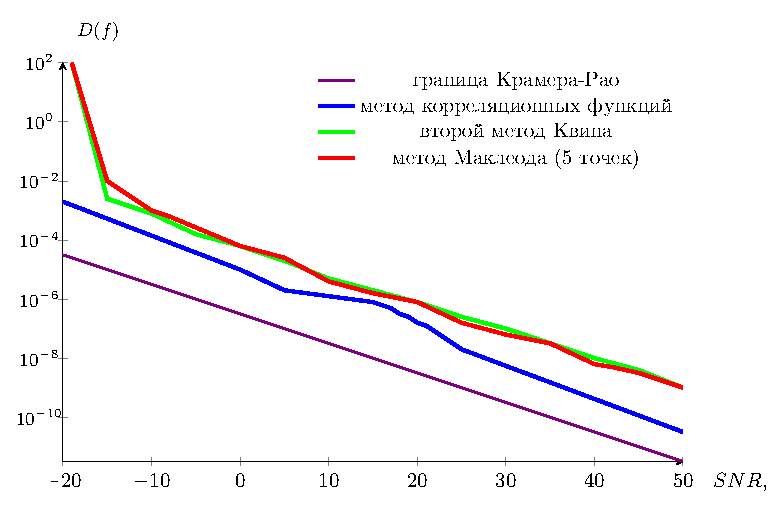
\includegraphics [scale=0.9] {Cramer_Rao.pdf}
	\caption{Дисперсия при оценке основной частоты напряжения.}
	\label{img:picture1.4}
\end{figure}

\begin{table} [htbp]
	\centering
	\changecaptionwidth\captionwidth{16cm}
	\caption{Название таблицы}\label{tab:Ts}%
	\begin{tabular}{| p{4cm} || p{6cm} | p{6cm} |}
		\hline
		\hline
		Название & Действительные значения & Комплексные значения \\
		\hline
		Случайные переменные & X & $\widetilde{X}=U+jV (U and V independent)$ \\
		\hline
		Значение & $E{[}x{]} = \int xp(x)dx$ & $E[\widetilde{X}]=\int up_U (u)du+j\int up_V(\upsilon)d\upsilon$ \\
		\hline 
		Дисперсия &  
		$var(X)=E[(X-E[X]^2) \linebreak =\int(x-E[x])^2px(x)dx$   & 
		$var(\widetilde{X})=E[|\widetilde{X}-E[\widetilde{X}]|^2]  =\int |\widetilde{x}-E[\widetilde{X}]|^2pU,V(u,\upsilon)dud\upsilon$ \\
		\hline
		Нормальное распределение &
		$px(x)=\frac{1}{\sqrt{2\pi\sigma^2}} exp [-\frac{1}{2\sigma^2}(x-\mu)^2]$  
		& $p\widetilde{x}(\widetilde{x})=\frac{1}{\sqrt{2\pi\sigma^2}} exp [-\frac{1}{2\sigma^2}|\widetilde{x}-\widetilde{\mu}|^2]$	\\
		\hline
		Свертка & $cov(X,Y)=E[(X-E[X])(Y-E[Y])]$  
		& $cov(X,Y)=E[(\widetilde{X}-E[\widetilde{X}])(\widetilde{Y}-E[\widetilde{Y}])]$ \\
		\hline
		Произвольный вектор &$X=[X_1X_2...X_L]^T$            
		&$X=[\widetilde{X}_1\widetilde{X}_2...\widetilde{X}_L]^T$ \\
		\hline
		Среднее значение вектора &$E[X]=[E[X_1]E[X_2]...E[X_L]]^T$ 
		&$E[\widetilde{X}]=[E[\widetilde{X}_1]E[\widetilde{X}_2]...E[\widetilde{X}_L]]^T$ 
		\\
		\hline
		Матрица свертки  &$C_x=E[(X-E[X])(X-E[X])^T]$ $(C_x^T =C_x)$    
		&$C_x=E[(X-E[X])(X-E[X])^H]$ $(C_x^H =C_x)$ \\
		\hline
		Многомерное нормальное распределение &$px(x)=\frac{1}{(2\pi)^(L/2) det^(1/2)(C_x)}$ $.exp[\frac{1}{2}(x-\mu)^T C_x^(-1)(x-\mu)]$  
		&$p\widetilde{x}(\widetilde{x})=\frac{1}{(\pi)^L det(C_x)}$ 
		\linebreak
		$.exp[-(\widetilde{x}-\widetilde{\mu})^H C_x^(-1)(\widetilde{x}-\widetilde{\mu})]$ \\
		\hline
		Автокорреляция &$r_x[k]=E[x[n]x[n+k]]$        
		&  $r_x[k]=E[x^*[n]x[n+k]]$ \\
		\hline
		Cпектральная плотность мощности & $P_x(f)=\Sigma_k^\infty=\infty r_x[k](-j2\pi fk)$  
		$(P(-f)=P_x(f))$               
		& $P_x(f)=\Sigma_k^\infty=\infty r_x[k](-j2\pi fk)$ \\
		\hline
		Аддитивный белый гауссовский шум & $w{[}n{]}$                       
		&$\widetilde{w}[n]=u[n]+j\upsilon[n]  
		(u[n),\upsilon[n]$ \linebreak) \\
		\hline
		Авторегрессионный метод &
		$x[n]=-\Sigma_k^p a[k]x[n-k]+u[n] (u[n] is WGN)$
		& $\widetilde{x}[n]=-\Sigma_k^p a[k]\widetilde{x}[n-k]+\widetilde{u}[n]$  \linebreak  
		($a[k]^s$ complex and $u[n]$ is CWGN) \\
		\hline
		\hline
	\end{tabular}
\end{table}



\section{Модель сигнала электрической сети} \label{sec:ch1/sec6}
% МОДЕЛЬ СИГНАЛА ЭЛЕКТРИЧЕСКОЙ СЕТИ ДЛЯ ИЗМЕРЕНИЯ ГАРМОНИК И ИНТЕРГАРМОНИК

Гармоника -- это спектральная составляющая на частотах, которая кратна основной частоте системы переменного тока. 

Интергармоника -- это спектральная компонента на частотах, которая зависит от единиц измерения и не кратна основной частоте системы.
Основополагающим нормативным документом в РФ, регламентирующим отличие между гармониками и интергармониками, является государственный стандарт \cite{GOST30804.4.7-2013}. 
%ГОСТ 30804.4.7-2013 (IEC 61000-4-7:2009) Совместимость технических средств электромагнитная. Общее руководство по средствам измерений и измерениям гармоник и интергармоник для систем электроснабжения и подключаемых к ним технических средств. 2013; Доступно по: http://docs.cntd.ru/document/1200103652 

Стандарт  описывает спектральные составляющие тока и напряжения, расположенных выше области частот гармоник $2-9$ кГц. Определение терминов «гармоника» и «интергармоника» в стандарте \cite{GOST30804.4.7-2013}, в разделах $3.2.3$ и $3.4.2$.

Согласно стандарту \cite{GOST32144-2013}, раздел $3.1.19$, под «напряжением интергармонической составляющей» понимают среднеквадратическое значение синусоидального напряжение, частота которого не кратна основной частоте напряжения электропитания.
%ГОСТ 32144-2013 Электрическая энергия. Совместимость технических средств электромагнитная. Нормы качества электрической энергии в системах электроснабжения общего назначения. 2013; Доступно по: http://docs.cntd.ru/document/1200104301 
Если одновременно возникнут интергармонические составляющие на приближенных частотах, то образуется напряжение с широкополосным спектром. В разделе $4.2.4.2$ настоящего стандарта описано, что «допустимые уровни интергармонических составляющих напряжения электропитания находятся на рассмотрении».

В международной электротехнической комиссии (МЭК, IEC -- International Electrotechnical Commission) стандартизация в области интергамоник находится на рассмотрении и накоплении информации. В стандарте [3] интергармоники напряжения ограничиваются значением $0,2\%$.
%3. International Electrotechnical Commission et al. Electromagnetic Compatibility (EMC)-Part 4-7: Testing and Measurement Techniques-General Lighting Res. Technol. 2013; 45: 710–728 Guide on Harmonics and Interharmonics Measurements and Instrumentation, for Power Supply Systems and Equipment Connected Thereto. – IEC 61000-4. – Т. 7.

Кроме Российских стандартов, существуют международные регламентирующие документы по мониторингу качества электроэнергии (КЭ), рекомендация от Института инженеров электротехники (IEEE – Institute of Electrical and Electronics Engineers). Термин гармоника в \cite{6826459} обозначают как «total harmonic distortion (THD)».
% 4. IEEE Recommended Practice and Requirements for Harmonic Control in Electric Power Systems, in IEEE Std 519-2014 (Revision of IEEE Std 519-1992), vol., no., pp.1-29, 11 June 2014, doi: 10.1109/IEEESTD.2014.6826459. Доступно по: https://ieeexplore.ieee.org/servlet/opac?punumber=6826457 (дата обращения: 01.10.2020).
То есть отношение среднеквадратичного значения гармонического содержимого с учетом гармонических составляющих до $50$-го порядка, исключая интергармоники. Пороговые значения интергармоник в сетях низшего (до $1$ кВ), среднего ($69-161$ кВ) и высшего (более $161$ кВ) напряжения.

Наличие интергармоник и гармоник оказывает негативное влияние на оборудование. Из-за возникновения гармоник в электрических сетях происходит перегрев оборудования, поэтому уменьшается его срок службы. Интергармоники наблюдаются при увеличении количества нагрузок в дополнение к гармоникам. Наличие асинхронных включений частотно-регулируемых электроприводов, выполненных на основе полупроводниковых преобразователей является причиной появления интергармоник. Так же интергамоники возникают при изменении тока в оборудовании, которое приводит к колебаниям напряжения. 

Источниками интергармоник в электрических сетях являются асинхронные включения частотно-регулируемых электроприводов, дуговые печи, частотно регулируемые электроприводы. 

Возникновение интергармоник обусловлено модуляцией несинусоидальных процессов, кривые которых содержат только кратные высшие гармоники, а также низкочастотные колебания, характерные для сетей с резко переменными нагрузками. Например, электродуговые сталеплавильные печи, сварочные установки, тиристорные электроприводы \cite{Interharmonics_in_systems_Zhezhelenko_1999}. В зависимости от амплитуды токов высших гармоник возникают искажения напряжения в узлах нагрузок на данной частоте. Повышается вероятность возникновения резонанса, в зависимости от ширины спектра частот интергармоник. 
%5. Жежеленко И. В., Саенко Ю. Л., Бараненко Т. К. Интергармоники в системах электроснабжения промпредприятий //Вестник Приазовского государственного технического университета. Серия: Технические науки. 1999;8. Доступно по: https://cyberleninka.ru/article/n/intergarmoniki-v-sistemah-elektrosnabzheniya-prompredpriyatiy 

В состав промышленных предприятий входят частотно-регулируемые электроприводы. Известно, что данные установки являются характерным источником высших гармоник и генерируют гармоники $5,7,11,13$ и другие. Эти гармоники также генерируются сварочными выпрямителями \cite{Calculation_Current_Mikheev_2017}. Высшие гармоники также называют каноническими гармониками.

%Михеев Г. М. и др. Расчет тока конденсаторных батарей с учетом источников высших гармоник //Вестник Чувашского университета. 2017; 1. Доступно по: https://cyberleninka.ru/article/n/raschyot-toka-kondensatornyh-batarey-s-uchetom-istochnikov-vysshih-garmonik
Проблема измерения гармоник и интергармоник в электрической сети является актуальной. \cite{testa2007интергармоники, gunther2001interharmonics, 532851, testa2002interharmonic}

%7. A. Testa et al., «Interharmonics: Theory and Modeling,» in IEEE Transactions on Power Delivery, vol. 22, no. 4, pp. 2335-2348, Oct. 2007, doi: 10.1109/TPWRD.2007.905505. Доступно по: https://ieeexplore.ieee.org/document/4302786/references#references (дата обращения: 01.10.2020).
%8. E. W. Gunther, «Interharmonics in power systems» 2001 Power Engineering Society Summer Meeting. Conference Proceedings (Cat. No.01CH37262), Vancouver, BC, Canada, 2001, pp. 813-817 vol.2, doi: 10.1109/PESS.2001.970156. Доступно по: https://ieeexplore.ieee.org/document/970156 (дата обращения: 01.10.2020).
%9. R. Yacamini, «Power system harmonics. IV. Interharmonics» in Power Engineering Journal, vol. 10, no. 4, pp. 185-193, Aug. 1996, doi: 10.1049/pe:19960411. https://ieeexplore.ieee.org/document/532851  Доступно по:  (дата обращения: 01.10.2020).
%10. Gallo D., Langella R., Testa A. Interharmonic measurement in IEC framework //IEEE Summer Power Meeting. 2002. Доступно по: https://iris.unicampania.it/handle/11591/206785#.XoBAHogzZPY (дата обращения: 01.10.2020).
 
Спектральный анализ гармоник и интергармоник так же представлен в отечественных работах. \cite{Improving_methods_Shizma_2014,Harmonic_analysis_Goldstein2009, Development_method_Osipov_2017}

%11.Чижма С. Н. Совершенствование методов и средств контроля качества электроэнергии и составляющих мощности в электроэнергетических системах с тяговой нагрузкой //Омск: Омский государственный университет путей сообщения. 2014; Доступно по: https://omgtu.ru/scientific_activities/dissertatsionnye_sovety/obyavleniya_o_zashchite_dissertatsiy_i_dokumenty_k_nim/chizhma_s_n/ (дата обращения: 01.10.2020).
%12.  Гольдштейн Е. И., Радаев Е. В. Гармонический анализ токов (напряжений) при наличии в них интергармоник и неизвестном периоде результирующего сигнала //Электричество. – 2009. – №. 12. – С. 87-88.
%13. Осипов Д. С. и др. Разработка метода расчета потерь мощности в токоведущих частях при наличии интергармоник //Омский научный вестник. – 2017. – №. 4 (154). 


В \cite{Improving_methods_Shizma_2014} рассмотрен метод канонических гармоник и интергармоник. Реализация с помощью оконного преобразования Фурье (ОПФ) с применением оконных функций низкого разрешения и интерполяции. 
%11.Чижма С. Н. Совершенствование методов и средств контроля качества электроэнергии и составляющих мощности в электроэнергетических системах с тяговой нагрузкой //Омск: Омский государственный университет путей сообщения. 2014; Доступно по: https://omgtu.ru/scientific_activities/dissertatsionnye_sovety/obyavleniya_o_zashchite_dissertatsiy_i_dokumenty_k_nim/chizhma_s_n/ (дата обращения: 01.10.2020).


Авторы \cite{Harmonic_analysis_Goldstein2009} работы перед проведением дискретного преобразования Фурье (ПФ) предложили догармонический анализ сигнала. Т.е. предварительное определение частот, входящих в исходный сигнал путем расчета среднеквадратичного отклонения, определение периода сигнала электрической сети путем нахождения общего делителя. 
%12.  Гольдштейн Е. И., Радаев Е. В. Гармонический анализ токов (напряжений) при наличии в них интергармоник и неизвестном периоде результирующего сигнала //Электричество. – 2009. – №. 12. – С. 87-88.


В \cite{Development_method_Osipov_2017} разработан алгоритм расчета дополнительных потерь в токоведущих частях при наличии интергармоник, генерируемых частотно-регулируемым приводом на основе пакетного вейвлет-преобразования (ПВП).
%13. Осипов Д. С. и др. Разработка метода расчета потерь мощности в токоведущих частях при наличии интергармоник //Омский научный вестник. – 2017. – №. 4 (154). 

Спектральные составляющие на частотах, расположенных между двух последовательных гармонических частот, возникают при наличии в сигнале интергармонических составляющих. 
Заметные интергармоники появляются в узком диапазоне частот: $35$ – $75$ Гц, $150$ – $160$ Гц \cite{Interharmonics_in_systems_Zhezhelenko_1999}.
% Жежеленко И. В., Саенко Ю. Л., Бараненко Т. К. Интергармоники в системах электроснабжения промпредприятий //Вестник Приазовского государственного технического университета. Серия: Технические науки. 1999;8. Доступно по: https://cyberleninka.ru/article/n/intergarmoniki-v-sistemah-elektrosnabzheniya-prompredpriyatiy 
 
Модель сигнала электрической сети с учетом \cite{GOST30804.4.7-2013}, раздел $3.1$, связывает гармоники, высшие гармоники и интергармоники тока и напряжения электрической сети при наличии шума: 
%ГОСТ 30804.4.7-2013 (IEC 61000-4-7:2009) Совместимость технических средств электромагнитная. Общее руководство по средствам измерений и измерениям гармоник и интергармоник для систем электроснабжения и подключаемых к ним технических средств. 2013; Доступно по: http://docs.cntd.ru/document/1200103652
\begin{equation}
	\label{eq:equation6}
		s_{t} = a_{0} \sin (\omega_{0} t + \varphi_{0}) + \displaystyle\sum_{p=0}^{p} a_p^{\upsilon} \sin (m_p^{\upsilon} \omega_{0} t + \varphi_p^{\upsilon}) + \displaystyle\sum_{q=0}^{q} a_q^i \sin  (\omega_q^i t + \varphi_q^{i})
\end{equation}

где $a_{0}$ – амплитуда первой гармоники;

$\omega_{0}$ – угловая частота первой гармоники, $\omega_{1} = 2 \pi f_{H,1}$;

$\varphi_{0}$ – фаза первой гармоники; 

$p$ – число высших гармоник;

$a_p^{\upsilon}$ – амплитуда высших гармоник;

$m_p^{\upsilon}$ – номер высших гармоник;

$\varphi_p^{\upsilon}$ – фаза высших гармоник;

$q$– номер интергармоник;

$a_q^i$ – амплитуда интергармоник;

$\omega_q^i$ – угловая частота интергармоник, $\omega_q^i=2\pi f_{ig,h}$; 

$f_{ig,h}$ – частота интергармонической подгруппы порядка $h$;

$\eta$ – шум.

В формулу \ref{eq:equation6} добавлены значения высших гармоник, интергармоник тока и напряжения электрической сети.
Согласно \cite{GOST32144-2013}, раздел $4.2.4$, к показателям качества электрической энергии (КЭ), относятся гармонические составляющие напряжения, т.~е. коэффициент  $n$ гармонической составляющей напряжения – $K_{U(n)}$:
%ГОСТ 32144-2013 Электрическая энергия. Совместимость технических средств электромагнитная. Нормы качества электрической энергии в системах электроснабжения общего назначения. 2013; Доступно по: http://docs.cntd.ru/document/1200104301 

\begin{equation}
	\label{eq:equation7}
K_{U(n)} = \frac{U_{(n)}}{U_1}
\end{equation}

где $n$ – номер гармонической составляющей напряжения;
 
$U_{(n)}$ – фазное напряжение гармоники в расчетной точке сети, В,кВ;

$U_1$ – значение основной гармонической составляющей напряжения, В,кВ.

\begin{equation}
	\label{eq:equation8}
	U_(n) = \frac{I_{(n)} n U_{nl} U_{nom}}{S_k}
\end{equation}

где n – номер гармонической составляющей напряжения;

$I_{(n)}$ – действующее значение фазного тока -ой гармоники, А,кА;

$U_{nl}$ – напряжение нелинейной нагрузки (в случае, если расчетная точка совпадает с точкой присоединения нелинейной нагрузки $U_{nl} = U_{nom}$, В,кВ;

$U_{nom}$ – номинальное напряжение сети, В,кВ;

$S_k$ – мощность короткого замыкания в точке присоединения нелинейной нагрузки, кВ А.

Значения коэффициентов нечетных гармонических составляющих напряжения не кратных трем $K_{U(n)}=0,4$ \% $U_1$ для $n>25$, при напряжении электрической сети $110-220$ кВ.

Значения коэффициентов нечетных гармонических составляющих напряжения кратных трем $K_{U(n)}=0,2$ \% $U_1$ для $n>21$, при напряжении электрической сети $110-220$ кВ.

Значения коэффициентов четных гармонических составляющих напряжения $K_{U(n)}=0,2$ \% $U_1$ для $n>21$, при напряжении электрической сети $110-220$ кВ.
Согласно \cite{GOST32144-2013}, раздел $4.2.4$, «Допустимые уровни интергармонических составляющих напряжения электропитания находятся на рассмотрении».
%2. ГОСТ 32144-2013 Электрическая энергия. Совместимость технических средств электромагнитная. Нормы качества электрической энергии в системах электроснабжения общего назначения. 2013; Доступно по: http://docs.cntd.ru/document/1200104301

Абсолютное значение амплитуды интергармоник $a_q^i$ изменяется в диапазоне $0,4-1$ для частоты $60$ Гц и $90$ Гц \cite{testa2007интергармоники}.
%7. A. Testa et al., «Interharmonics: Theory and Modeling,» in IEEE Transactions on Power Delivery, vol. 22, no. 4, pp. 2335-2348, Oct. 2007, doi: 10.1109/TPWRD.2007.905505. Доступно по: https://ieeexplore.ieee.org/document/4302786/references#references

В \cite{Improving_methods_Shizma_2014, ramos2017power}описаны принципы построения многофункциональных измерительных комплексов для электроподвижного состава и тяговых подстанций.
% 11. Чижма С. Н. Совершенствование методов и средств контроля качества электроэнергии и составляющих мощности в электроэнергетических системах с тяговой нагрузкой //Омск: Омский государственный университет путей сообщения. 2014; Доступно по: https://omgtu.ru/scientific_activities/dissertatsionnye_sovety/obyavleniya_o_zashchite_dissertatsiy_i_dokumenty_k_nim/chizhma_s_n/
% 14. Ramos C. J., Martins A. P., da Silva Carvalho A. Power system frequency estimation using a least mean squares differentiator //International Journal of Electrical Power & Energy Systems. 2017;87:166-175. Доступно по: https://www.sciencedirect.com/science/article/abs/pii/S0142061516315587. DOI: 10.1016/j.ijepes.2016.11.001
Наличие высокочастотных составляющих в сигналах токов и напряжений, определяют кривые первичных токов и напряжений электровоза с помощью прибора ИВК «Омск-М». Испытания проводились в Абаканской дистанции электроснабжения Красноярской дирекции по энергообеспечению. Анализ гармонических составляющих для спектра гармоник напряжений показал, что процент от амплитуды $1$-й гармоники от $5$ гармоники, будет равен $8$. И процент от амплитуды $1$-й гармоники будет равен $100$ на $2$ гармоники для спектра гармоник токов.

Анализ и контроль гармоник сигнала в электрической сети имеет большое значение для поддержания качества электрической энергии, предотвращения повреждения систем электрических сетей и экономии энергии. 

В работе представлена математическая модель сигнала в электрической сети, обобщающая результаты исследований проблем качества электроэнергии и учитывающая требования регламентирующих документов. Она позволяет проводить исследования алгоритмов анализа электрических сигналов, а также средств измерений, построенных на их основе.

\section{Выводы по разделу} \label{sec:ch1/sec7} 

В результате анализа, произведенного в первом разделе, можно сделать следующие выводы:
\begin{itemize}
\item Особенности сигналов в электрических сетях носят не существенный характер с точки зрения построения алгоритмов нахождения параметров гармоник. При работе с электрическими сетями обычно используют стандартные алгоритмы такого рода.

\item Помимо обычных алгоритмов для оценки параметров гармоник в электрических сетях также используют алгоритмы, анализирующие сигналы в переходных режимах, т.е. такие, в которых во время работы алгоритма может измениться значение какого-либо параметра. В нашей работе такие алгоритмы далее рассматриваться не будут, поскольку переходные режимы не являются целью нашей работы.

\item Анализ имеющихся библиографических источников показывает, что нет известных публикаций в которых бы велась разработка алгоритмов, ориентированных на работу при определенном соотношении сигнал-шум, и что для анализа гармоник и интергармоник (для которых это соотношение отличается) применяются одинаковые алгоритмы.

\item Алгоритмы оценки параметров гармоник, применяемые при работе с одно- и многотональными сигналами, имеют точность оценки параметров ниже теоретической границы Крамера-Рао. Вопрос о причинах снижения точности и возможности построения алгоритма, достигающего этой границы в известных научных публикациях не рассмотрен.

\item Для решения задачи построения оптимального алгоритма для анализа спектра сигнала в электрических сетях необходимо уточнение математической модели спектра сигналов в части, описывающей точность оценки (дисперсию) параметров гармоник спектра многотонального сигнала.
\end{itemize}

           % Глава 1
%[154. - Yue Yi, Zhiqiang Liu, Rong Guo, Ruichen Sun. Design and Implementation of Digital Power Quality Analyzer. – 2016.]

\chapter{Система анализа данных} \label{ch:ch2}

\section{Многопоточность} \label{sec:ch2/sec1}
% Разобраться в том, что такое многопоточность

Система анализа данных(Data analysis System) принимает точные данные из системы сбора и анализа данных. Эта подсистема в основном состоит из частот, гармоник, алгоритма анализа мощности и многопоточности (multi-threading) для повышения эффективности функционирования системы. 

Многопоточность была использована из-за следующих причин:
\begin{enumerate}
	\item Во-первых,АЦП DPQA должны взаимодействовать с пользователями, а это значит, что GUI (Графический Интерфейс Пользователя) должен реагировать за любые внутренние и внешние события. Если применяется последовательное программирование, пользователь может взаимодействовать только с АЦП DPQA, после того как программа завершилась. 
	
	\item Во-вторых, с АЦП DPQA требуется непрерывно получать данные, как только была нажата кнопка «Старт». Многопоточность представляет собой оптимальный способ, чтобы обеспечить обработку данных и одновременного их получения. В заключение, больше времени эффективно применять многопоточность для анализа алгоритмов с участием нескольких операций (т.~е. оконные функции – windowing, промежуточные – padding, FFT и кросс-корреляцию – cross-correlation). 
\end{enumerate}

\section{Алгоритмы расчета частоты} \label{sec:ch2/sec2}

Чтобы рассчитать информацию о качестве электроэнергии, вычисляем сначала входную частоту. Существуют три альтернативных метода для вычисления частоты по дискретизированному сигналу(sampled signal):
\begin{itemize}
	\item Пересечение (Zero-Crossing).
	\item Максимальная точка (Maximum-Point).
	\item Дискретное преобразование Фурье (ДПФ).
\end{itemize}
Метод ДПФ (FFT) используется для вычисления входных значений частоты. Формула ДПФ описана [152]:
% [152 - Sundararajan D. The discrete Fourier transform: theory, algorithms and applications. – World Scientific, 2001.]
\begin{equation}
\label{eq:equation1}
X(k) = \frac{1}{N} \sum\limits_{n=0}^{N-1} x(n)e^{-j\frac{2 \pi}{N}nk}
\end{equation}

где $N$ -- это число $k = 0, 1, \cdots, N-1$

Для реализации ДПФ в Python используем алгоритм быстрого преобразования Фурье (БПФ, FFT). БПФ -- это эффективный алгоритм для вычисления ДПФ (DFT). Число операций необходимых для вычисления Дискретного преобразования Фурье пропорционально $N2$ и $N$ наблюдений при этом алгоритм БПФ требует число операций пропорциональное $Nlog(N)$ [153].
% [153 -	Cooley J. W., Lewis P. A. W., Welch P. D. The fast Fourier transform and its applications //IEEE Transactions on Education. – 1969. – Т. 12. – №. 1. – С. 27-34.]
После того, как реализовали алгоритм вычисления частоты, произошли проблемы разрешением частоты. Для обнаружения потоков сигналов в частотной области,  требуются улучшения разрешения. Сигнал частотной области, рассчитанный БПФ, имеет разрешение $0,5$~Гц. В результате, любое содержимое сигнала, которое существует между двух частот  с разделением $0,5$~Гц, будет полностью игнорироваться, и будет вызван неправильный результат частоты.

Следовательно, разрешение по частоте должно быть улучшено, чтобы минимизировать ошибку вычисления. Используем ноль заполнение для улучшения разрешения БПФ. Из уравнения видно, что длина $X(k)$ полностью зависит от количества образцов $X (n)$.

Текущий сигнал задается уравнением:
\begin{equation}
\label{eq:equation2}
I = R_{HallEffect} \times  I_{ADC} + Offset
\end{equation}

где $R_{HallEffect}$ -- коэффициент выхода напряжения на эффекте Холла;

$I_{ADC}$ -- необработанные текущие данные из АЦП, добавлено смещение, постоянное смещение от схемы регулировки;

Модификация сигнала напряжения:
\begin{equation}
\label{eq:equation3}
V = R_Trans former\times V_ADC + Offset
\end{equation}
где $R_Trans former$ -- Коэффициент обмотки трансформатора;
$V_{ADC}$ -- представляет собой исходные данные напряжения от АЦП;

Из уравнения \labelcref{eq:equation2} длина волны $X(k)$ зависит от количества образцов $X(n)$. Если добавлять нули в конец $X(n)$, способны эффективно увеличить количество образцов $X(n)$ без изменения фактического сигнала. Это будет также увеличивать размер $X(k)$. $X(k)$ не меняется, потому что $X(n)$ остается прежним сигналом. Приращение частоты bins из $X(k)$ мы будем сжимать bins ближе к друг другу, который дает разрешение по частоте.

\section{Алгоритмы вычисления амплитуды гармоник} \label{sec:ch2/sec3}

Содержание гармоник до $20$ гармоники. Содержание гармоник можно извлечь из частотного спектра, после того как мы получили основную частоту БПФ (FFT) напряжения и текущего значения. Гармоники расположены в частотной области, которые являются положительными целыми числами, кратными основной частоте. Чтобы получить гармоники используем частотный индекс и умножаем его на целые числа. После этого берем амплитуды тока и напряжения от БПФ (FFT) на основе рассчитанного индекса. Результаты гармоник не точные (из результатов тестирования). Причина заключается в том, что измеренный нами сигнал ограничен по времени. При выполнении БПФ (FFT), есть частота сглаживания (frequency aliasing). Если заполнять нулями массив, то длина данных увеличивается, и гармоника может не располагать точным частотным индексом (из-за ошибок в вычислениях).

Чтобы решить проблему, вместо использования рассчитанного индекса для получения амплитуды гармоник, ищем индексы. Находим максимальную точку в этом индексе. Тогда максимальная амплитуда будет точкой максимальной амплитуды в пределах диапазона.

\section{Коэффициент мощности и алгоритм расчета энергопотребления} \label{sec:ch2/sec4}

Для нахождения коэффициента мощности была применена перекрестная корреляция (Cross Correlation), а также идентификация триггера (Trig Identity). Перекрестная корреляция нужна для того, чтобы найти более точные результаты идентификации триггера вместо взаимной корреляции. Рассмотрим два сигнала, первый сигнал представляет напряжение из уравнения \labelcref{eq:equation4}, другой~–-~ток из уравнения 

\labelcref{eq:equation5}:
\begin{equation}
\label{eq:equation4}
V = A \cos(\omega t)
\end{equation}

\begin{equation}
\label{eq:equation5}
I = B \cos (\omega t + \theta)
\end{equation}

Ток содержит разность фаз $\theta$. Умножение двух сигналов вместе дает \labelcref{eq:equation6}:

\begin{equation}
\label{eq:equation6}
\left| {V \times I}\right| = \left|A \right| \times \left|B \right| \times \cos \theta  
\end{equation}

Разность фаз может быть найдена как \labelcref{eq:equation7}:

\begin{equation}
\label{eq:equation7}
\theta = \cos^{-1} \frac{V \times I}{A \times B}  
\end{equation}

Уравнение \labelcref{eq:equation7} можно записать в дискретной форме:

\begin{equation}
\label{eq:equation8}
\theta = \cos^{-1} \frac{\sum V\left[ n \right] I\left[ n \right]}{\sqrt{\sum{{\left| V\left[ n \right]\right|}^2} \sum{{\left| I\left[ n \right]\right|}^2}}}
\end{equation}

Функция обратного косинуса может возвращать величину $\theta$, которая означает полярность коэффициента мощности. Чтобы найти полярность коэффициента мощности, используется кросс-корреляцию:

\begin{equation}
\label{eq:equation9}
R_{VI}(l) = \sum_{n=-\infty}^{\infty}V(n)I(n-l)
\end{equation}
где $l=0,\mp1,\mp2,\dots$

$R_{VI}(l)$ -- является наибольшим $l$, в котором напряжение и ток сигнала имеют наибольшее сходство.

Знак перед $l$ показывает является ли коэффициент мощности нагрузки опережающим или запаздывающим. Отрицательное $l$ означает, что текущий сигнал смещен влево. Интервал выборки характеризует отстающую нагрузку. Положительное значение $l$ означает, что нагрузка является ведущей нагрузкой, $l=0$ говорит о том, что нагрузка резитивная (purely resistive). Получение коэффициента мощности позволит рассчитать потребляемую мощность нагрузки.

Из алгоритма нахождения гармоник и амплитуд находим амплитуду содержания гармоник и рассчитываем реальную реактивную мощность в уравнениях (\labelcref{eq:equation10} и \labelcref{eq:equation11}):

\begin{equation}
\label{eq:equation10}
P_{real} = I\times V \cos \theta
\end{equation}

\begin{equation}
\label{eq:equation11}
P_{reactive} = I\times V \sin \theta
\end{equation}

\section{Интерполированные алгоритмы ДПФ с нулевым заполнением для классических окон} \label{sec:ch2/sec5}
% [155. - Luo J., Xie Z., Xie M. Interpolated DFT algorithms with zero padding for classic windows //Mechanical Systems and Signal Processing. – 2016. – Т. 70. – С. 1011-1025.]

Точная оценка параметров (частоты, амплитуды и фазы) для синусоид, загрязненных случайным шумом (random noise), была предметом исследований в различных областях в течение нескольких десятилетий. Например, общая проблема, возникающая при анализе вибрации для вращающихся машин является оценкой параметров дискретизированных многочастотных сигналов в присутствии аддитивного шума (additive noise) [156].

% [156. - Santamaria I., Pantaleon C., Ibanez J. A comparative study of high-accuracy frequency estimation methods //Mechanical Systems and Signal Processing. – 2000. – Т. 14. – №. 5. – С. 819-834.]

С увеличением применения в нелинейных устройствах (non-linear devices) и периодических временных переменных нагрузок в электроэнергетических системах, искажение тока и напряжения сигналов (voltage waveforms) становится серьезной проблемой. Поэтому анализ и контроль гармоник электрической мощности в реальном времени имеет большое значение для поддержания качества электрической энергии (electrical energy), предотвращения повреждения систем электрических сетей (network systems) и экономии энергии (saving energy)[157][158].

% [157.- Zhang F., Geng Z., Yuan W. The algorithm of interpolating windowed FFT for harmonic analysis of electric power system //IEEE transactions on power delivery. – 2001. – Т. 16. – №. 2. – С. 160-164.]

%[158.- Qian H., Zhao R., Chen T. Interharmonics analysis based on interpolating windowed FFT algorithm //IEEE Transactions on Power Delivery. – 2007. – Т. 22. – №. 2. – С. 1064-1069.]
Кроме того, ряд аудио кодирования (audio coding) технологий были недавно разработан, где звуковой сигнал (audio signal) раскладывается на синусоиды и шума перед кодированием. Разложение (decomposition), конечно, зависит от точной оценки частоты (frequency estimation) звукового сигнала [159]. 
% [159.- Ferreira A., Sinha D. Accurate and robust frequency estimation in the ODFT domain //IEEE Workshop on Applications of Signal Processing to Audio and Acoustics, 2005. – IEEE, 2005. – С. 203-206.]

В предшествующей литературе были представлены различные подходы к оценке, которые обычно можно классифицировать на временную область и частотную область. Учитывая их простую работу и высокую эффективность, часто используются подходы в частотной области, основанные на дискретном преобразовании Фурье (discrete Fourier transform – DFT) и реализованные с помощью быстрого преобразования Фурье (fast Fourier transform – FFT). Тем не менее, существуют некоторые присущие методам частотной области недостатки, такие как эффект пикет-ограды (picket fence effect – PFE) и эффект спектральной утечки (spectral leakage effect – SLE) [158]. 
% [158. - Qian H., Zhao R., Chen T. Interharmonics analysis based on interpolating windowed FFT algorithm //IEEE Transactions on Power Delivery. – 2007. – Т. 22. – №. 2. – С. 1064-1069.]

Они могут вносить существенные ошибки в оценки частоты, если сигнал некогерентно дискретизирован (noncoherently sampled) [160][161].

Исследования показали, что если можно позволить себе дополнительные вычислительные затраты, можно компенсировать ошибки и получить высокоточные оценки частоты даже с небольшим количеством выборок [156].
% [156.- Santamaria I., Pantaleon C., Ibanez J. A comparative study of high-accuracy frequency estimation methods //Mechanical Systems and Signal Processing. – 2000. – Т. 14. – №. 5. – С. 819-834.]

Интерполированный алгоритм DFT (IpDFT) является одним из наиболее широко изученных методов оценки [156] ,[157], [158], [159], [160], [161],.[162], [163], [164], [165], [166], [167], [168], [169], [170], [171]. 
% [156.-Santamaria I., Pantaleon C., Ibanez J. A comparative study of high-accuracy frequency estimation methods //Mechanical Systems and Signal Processing. – 2000. – Т. 14. – №. 5. – С. 819-834.]

% [157.-Zhang F., Geng Z., Yuan W. The algorithm of interpolating windowed FFT for harmonic analysis of electric power system //IEEE transactions on power delivery. – 2001. – Т. 16. – №. 2. – С. 160-164.]

%[158.-Qian H., Zhao R., Chen T. Interharmonics analysis based on interpolating windowed FFT algorithm //IEEE Transactions on Power Delivery. – 2007. – Т. 22. – №. 2. – С. 1064-1069.]

%[159.	Ferreira A., Sinha D. Accurate and robust frequency estimation in the ODFT domain //IEEE Workshop on Applications of Signal Processing to Audio and Acoustics, 2005. – IEEE, 2005. – С. 203-206.]

%[160.-Xie M., Adams D. F. A nonlinear finite element analysis for composite materials //Finite elements in analysis and design. – 1996. – Т. 22. – №. 3. – С. 211-223.]

%[161.-Luo J., Xie M. Phase difference methods based on asymmetric windows //Mechanical Systems and Signal Processing. – 2015. – Т. 54. – С. 52-67.]

%[162.-Jain V. K., Collins W. L., Davis D. C. High-accuracy analog measurements via interpolated FFT //IEEE Transactions on Instrumentation and Measurement. – 1979. – Т. 28. – №. 2. – С. 113-122.]

% [163.-Grandke T. Interpolation algorithms for discrete Fourier transforms of weighted signals //IEEE transactions on instrumentation and measurement. – 1983. – Т. 32. – №. 2. – С. 350-355.]

%[164.-Andria G., Savino M., Trotta A. Windows and interpolation algorithms to improve electrical measurement accuracy //IEEE Transactions on Instrumentation and Measurement. – 1989. – Т. 38. – №. 4. – С. 856-863.]

%[165.-Offelli C., Petri D. Interpolation techniques for real-time multifrequency waveform analysis //6th IEEE Conference Record., Instrumentation and Measurement Technology Conference. – IEEE, 1989. – С. 325-331.]

%[166.-Agrez D. Weighted multipoint interpolated DFT to improve amplitude estimation of multifrequency signal //IEEE Transactions on Instrumentation and Measurement. – 2002. – Т. 51. – №. 2. – С. 287-292.]

%[167.-Jacobsen E., Kootsookos P. Fast, accurate frequency estimators [DSP Tips & Tricks] //IEEE Signal Processing Magazine. – 2007. – Т. 24. – №. 3. – С. 123-125.]

%[168.	Belega D., Dallet D. Multifrequency signal analysis by interpolated DFT method with maximum sidelobe decay windows //Measurement. – 2009. – Т. 42. – №. 3. – С. 420-426.]

%[169.-Belega D., Dallet D., Petri D. Accuracy of sine wave frequency estimation by multipoint interpolated DFT approach //IEEE Transactions on Instrumentation and Measurement. – 2010. – Т. 59. – №. 11. – С. 2808-2815.]

%[170.-Duda K. DFT interpolation algorithm for Kaiser–Bessel and Dolph–Chebyshev windows //IEEE Transactions on Instrumentation and Measurement. – 2011. – Т. 60. – №. 3. – С. 784-790.]

%[171.-Schoukens J., Pintelon R., Van Kamme H. The interpolated fast Fourier transform: A comparative study //[1991] Conference Record. IEEE Instrumentation and Measurement Technology Conference. – IEEE, 1991. – С. 358-364.]

Основная идея этого метода заключается в том, что частотная ошибка (frequency error) может быть компенсирована отношением средневзвешенного значения (weighted average) определенного числа известных спектральных бинов вокруг локального максимума. Когда максимум боковых лепестков (sidelobe) выбрано окно распада (MSDW, также известное как Райф-Винсент (Rife–Vincent) класс I окна), ошибка частоты может получить с помощью простых аналитических зависимосытей [166], [167], [168], [169]. 
%[166.-Agrez D. Weighted multipoint interpolated DFT to improve amplitude estimation of multifrequency signal //IEEE Transactions on Instrumentation and Measurement. – 2002. – Т. 51. – №. 2. – С. 287-292.]

%[167.-Jacobsen E., Kootsookos P. Fast, accurate frequency estimators [DSP Tips & Tricks] //IEEE Signal Processing Magazine. – 2007. – Т. 24. – №. 3. – С. 123-125.]

%[168.	Belega D., Dallet D. Multifrequency signal analysis by interpolated DFT method with maximum sidelobe decay windows //Measurement. – 2009. – Т. 42. – №. 3. – С. 420-426.]

%[169.-Belega D., Dallet D., Petri D. Accuracy of sine wave frequency estimation by multipoint interpolated DFT approach //IEEE Transactions on Instrumentation and Measurement. – 2010. – Т. 59. – №. 11. – С. 2808-2815.]

Основываясь на работе Оффелли (Offelli) и Петри (Petri) [165], 
%[165.-Offelli C., Petri D. Interpolation techniques for real-time multifrequency waveform analysis //6th IEEE Conference Record., Instrumentation and Measurement Technology Conference. – IEEE, 1989. – С. 325-331.]
Дуда (Duda) вывел алгоритм интерполяции полиномиального приближения (polynomial approximation interpolation – PAIpDFT), который можно использовать для окон Дольфа-Чебышева (Dolph–Chebyshev) и окон Кайзера-Бесселя (Kaiser–Bessel) [170]. 
%[170.-Duda K. DFT interpolation algorithm for Kaiser–Bessel and Dolph–Chebyshev windows //IEEE Transactions on Instrumentation and Measurement. – 2011. – Т. 60. – №. 3. – С. 784-790.]

Полиномиальные коэффициенты должны быть рассчитаны до анализа, что означает, что коэффициенты для различных окон должны быть рассчитаны и сохранены заранее. Этот процесс неизбежно является интенсивным и хлопотным, особенно для регулируемых окон, свойства которых могут регулироваться одним или несколькими параметрами.

Cначала рассмотрен новый алгоритм интерполяции для окна Хеннинга (Hanning window), в котором был принят метод заполнения нулями, чтобы получить больше спектральных линий (spectral lines) в пределах частотного интервала (frequency interval). Впоследствии этот новый алгоритм был расширен для совместимости с другими классическими окнами путем введения метода подгонки основного лепестка (main-lobe). Изучены систематические ошибки (systematic errors) предлагаемого метода для различных окон, а также характеристики при белом гауссовском шуме (white Gaussian noise).

\subsection{Основы алгоритма} \label{sec:ch2/sec5_1}

Рассмотрим для простоты, но без потери общности, непрерывный косинус-сигнал, загрязненный аддитивным белым шумом, который представлен в виде:
\begin{equation}
\label{eq:equation12}
x(t) = A_0 \cos(2 \pi f_0 t + \theta_0 + e(t))
\end{equation}

где $A_0$ – амплитуда;

$f_0$ – обозначает частоту;

$\theta_0$ – обозначает фазовый угол;

$t$ – обозначает переменную непрерывного времени;

$e(t)$ – белый шум. 

Отбор проб на частоте $f_s$ в течение интервала наблюдения (observation interval) $N\bigtriangleup t(\bigtriangleup t=1/f_s )$, следующий дискретный косинус сигнал $N$ образцы:
\begin{equation}
\label{eq:equation13}
x(n) = A_0 \cos(2 \pi \frac{f_0}{f_s} n + \theta_0) + e(n), n = 0,1, \cdots , N-1
\end{equation}

Чтобы удовлетворить теорему выборки Найквиста (Sampling Theorem), $f_s$ должно быть больше $2f_0$. Разрешение по частоте (Frequency resolution) получается $\bigtriangleup f=f_s/N$ определяется как:
\begin{equation}
\label{eq:equation14}
\frac{f_0}{f_s}=\frac{\lambda_0}{N}
\end{equation}

$\lambda_0$ – обозначает количество циклов, содержащихся в выборках сигнала (signal samples) [169].
%[169.-Belega D., Dallet D., Petri D. Accuracy of sine wave frequency estimation by multipoint interpolated DFT approach //IEEE Transactions on Instrumentation and Measurement. – 2010. – Т. 59. – №. 11. – С. 2808-2815.]

Следует подчеркнуть, что $\lambda_0$ также представляет нормированную частоту (частоту $f_0$, масштабированную по разрешающей способности по частоте), выраженную в бинах DFT [169].
%[169.-Belega D., Dallet D., Petri D. Accuracy of sine wave frequency estimation by multipoint interpolated DFT approach //IEEE Transactions on Instrumentation and Measurement. – 2010. – Т. 59. – №. 11. – С. 2808-2815.]
На этом этапе мы игнорируем шумовой член и переходим к умножению выборок сигнала $x(n)$ на значения окна данных $\omega(n)$.
Взвешенные образцы даны:
\begin{equation}
\label{eq:equation15}
x_\omega(n)=A_0 \cos(\frac{2 \pi \lambda_0 n}{N}+\theta_0)\omega(n)
\end{equation}

Дискретное преобразование Фурье (ДПФ, discrete Fourier transform – DFT) взвешенного сигнала может быть вычислена путем:
\begin{equation}
\label{eq:equation16}
X_\omega(k) = \sum_{n=0}^{N-1} x_\omega(n) e^{-j \frac{2 \pi}{N}nk}
\end{equation}

Применение \labelcref{eq:equation16} к взвешенным выборкам в \labelcref{eq:equation15} дает явный вид~(explicit form):

\begin{equation}
\label{eq:equation17}
X_\omega(k) = \frac{A_0}{2} e^{j\phi_0}W_N(k-\lambda_0)+\frac{A_0}{2}e^{j\phi_0}W_N(k+\lambda_0)
\end{equation}

где $W_N (k)$ и обозначает дискретное временное преобразование Фурье (discrete time Fourier transform – DTFT) весовой функции (weighting function). Если сигнал дискретизируется асинхронно, нормализованная частота $\lambda_0$ находится между двумя самыми большими спектральными линиями (spectral lines). Следовательно, $\lambda_0$  может быть далее записано на две части с целой частью $l_\omega$ и дробной частью (fractional part) $\delta_\omega$ $(-0,5<\delta_{\omega}\leq0,5)$ соответственно.

\begin{equation}
\label{eq:equation18}
\lambda_0 = l_\omega + \delta_\omega
\end{equation}

Целочисленная часть $l_\omega$ может быть легко и правильно определена с помощью процедуры максимального поиска, если SNR превышает пороговое значение (приблизительно от -$18$ до –$20$ дБ) [172]. 
% [172.-Rife D., Boorstyn R. Single tone parameter estimation from discrete-time observations //IEEE Transactions on information theory. – 1974. – Т. 20. – №. 5. – С. 591-598.]
Подстановка \labelcref{eq:equation18} в \labelcref{eq:equation17} дает наибольшую величину:
\begin{equation}
\label{eq:equation19}
\left|{X_\omega(l_\omega)} \right| = \frac{A_0}{2} \left| e^{j\phi_0}W_N(- \delta_\omega) +e^{j\phi_0}W_N(2l_\omega+\delta_\omega) \right| 
\end{equation}

Соответственно, вторая и третья по величине спектральные линии также могут быть определены. При правильной комбинации двух или более спектральных линий может быть получено отношение $\alpha$, которое зависит только от выбранного окна и отклонения частоты $\delta_{\omega}$. Другими словами, если окно данных, как известно, $\delta_{\omega}$ может быть определена только с помощью $\alpha$.

\begin{equation}
\label{eq:equation20}
\delta_\omega = g(\alpha)
\end{equation}

В частности, для максимальных окон распада боковых лепестков (side-lobe) $\delta_{\omega}$ можно записать как функцию от $\alpha$ в простой и явной форме [157], [158], [160], [161], [168], [169].

% [157. - Zhang F., Geng Z., Yuan W. The algorithm of interpolating windowed FFT for harmonic analysis of electric power system //IEEE transactions on power delivery. – 2001. – Т. 16. – №. 2. – С. 160-164.]

% [158.- Qian H., Zhao R., Chen T. Interharmonics analysis based on interpolating windowed FFT algorithm //IEEE Transactions on Power Delivery. – 2007. – Т. 22. – №. 2. – С. 1064-1069.]

% [160. - Xie M., Adams D. F. A nonlinear finite element analysis for composite materials //Finite elements in analysis and design. – 1996. – Т. 22. – №. 3. – С. 211-223.]

% [161.- Luo J., Xie M. Phase difference methods based on asymmetric windows //Mechanical Systems and Signal Processing. – 2015. – Т. 54. – С. 52-67]

% [168.-Belega D., Dallet D. Multifrequency signal analysis by interpolated DFT method with maximum sidelobe decay windows //Measurement. – 2009. – Т. 42. – №. 3. – С. 420-426.]

% [169.-Belega D., Dallet D., Petri D. Accuracy of sine wave frequency estimation by multipoint interpolated DFT approach //IEEE Transactions on Instrumentation and Measurement. – 2010. – Т. 59. – №. 11. – С. 2808-2815.]

Для других окон предлагается решение полиномиальной аппроксимации (polynomial approximation) [170]. 
%[170.	Duda K. DFT interpolation algorithm for Kaiser–Bessel and Dolph–Chebyshev windows //IEEE Transactions on Instrumentation and Measurement. – 2011. – Т. 60. – №. 3. – С. 784-790.]

В следующем разделе представляем простой алгоритм интерполяции (interpolation), который можно применять практически ко всем классическим окнам.

\subsection{Предлагаемый алгоритм} \label{sec:ch2/sec5_2}

Рассмотрим алгоритм техника заполнения нулями. Заполнение нулями – это метод, определяемый как добавление нулевых значений к взвешенным выборкам до вычисления DFT. Добавленные нулевые значения обрабатываются как дополнительные образцы, собранные с той же скоростью, и, следовательно, увеличивают время измерения, как показано в \labelcref{eq:equation21}

\begin{equation}
\label{eq:equation21}
x_{ap}(n)=
\begin{cases}
x_{\omega}, \leq n < N
\\ 0, N \leq n < MN
\end{cases}
\end{equation}

где $(M-1) \cdot N$ добавляются нули. Соответственно, дискретный спектр (discrete spectrum) также расширяется. Эта процедура приводит к более точной выборке спектра сигнала (signal spectrum), потому что вместо $N$ спектральных выборок $M \cdot N$ образцы того же спектра доступны. Обратите внимание, что расширение данных нулями и вычисление более длинного ДПФ действительно увеличивает количество точек в частотной области, но не нарушает основное ограничение и не влияет на эффекты наложения [173].
% [173.-Dorf R. C. Circuits, signals, and speech and image processing. – CRC Press, 2018.]

Пределы разрешения  (Resolution limits) определяются интервалом наблюдения (observation interval) и частотой дискретизации (sampling frequency) [173].

Никакое количество заполнения нулями не может преодолеть эти фундаментальные пределы, и параметры спектра, такие как уровень отношение сигнал/шум (signal-to-noise ratio) и уровень спектральной утечки (spectral leakage), остаются неизменными. Коэффициенты ДПФ по \labelcref{eq:equation21}:

\begin{equation}
\label{eq:equation22}
X(N)= \sum_{n=0}^{MN-1} x_{ap}(n) e^{-j \frac{2 \pi}{N}\cdot \frac{k}{M} \cdot n}, 0\leq k \leq MK-1
\end{equation}
По сравнению с \labelcref{eq:equation16} получается:

\begin{equation}
\label{eq:equation23}
X(k)= X_\omega \left( {\frac{k}{M}}\right)  \end{equation}
Соответственно, \labelcref{eq:equation19} можно переформулировать как:

\begin{equation}
\label{eq:equation24}
\left| {X(l)} \right|   = \frac{A_0}{2}\left| {e^{j\phi_0}W_N(-\delta)+e^{-j\phi_0}W_N \left(\frac{2l}{M}+\delta \right)} \right|,
\end{equation}

где $l$ и $\hat{\delta}
\left( {\delta= \frac{\hat{\delta}}{M}}\right) $
являются целой частью и дробная часть (fractional part) из $M\lambda_0$ соответственно. Точно так же $l$ возвращается максимальной процедурой поиска X(k). На этом этапе три крупнейших линии X(k) даны $\left| {X(l)} \right|$,$\left| {X(l+1)} \right|$ а также $\left|{X(l-1)}\right|$.

Рассмотрим алгоритм интерполяции для окна Хеннинга с техникой заполнения нулями.

Второе слагаемое в правой части \labelcref{eq:equation24} представляет вклад мнимой части (imaginary part) спектра. Если $\lambda_0$ удовлетворяет $5<\lambda_0$ , а также $\lambda_0 < \frac{N}{2}-5$, тогда помехи от второго слагаемого могут быть минимальными и ими можно пренебречь. С этим предположением \labelcref{eq:equation24} сводится к:

\begin{equation}
\label{eq:equation25}
\left| {X(l)} \right| \cong \frac{A_0}{2}\left| {W_N(-\delta)} \right|,
\end{equation}

Точно так же у нас есть это $\left| {X(l)} \right| \cong \frac{A_0}{2}\left| {W_N(\varepsilon -\delta)} \right|$, а так же $\left| {X(l-1)} \right| \cong \frac{A_0}{2} \left| {W_N(\varepsilon +\delta)} \right|$, где $\varepsilon=\frac{1}{M}$. Для окна Хеннинга (Hanning window), $W_N (k) \cong \frac{sin(\pi k)}{h(k)}$,
$h(k) = 2 \pi k (1-k^2)$ [160]
%[160.	Xie M., Adams D. F. A nonlinear finite element analysis for composite materials //Finite elements in analysis and design. – 1996. – Т. 22. – №. 3. – С. 211-223.]

\begin{equation}
\label{eq:equation26}
\left| {X(l)} \right| \cong \frac{A_0}{2} \frac{\sin{(\pi \delta)} }{h(\delta)} ,
\end{equation}

\begin{equation}
\label{eq:equation27}
\left| {X(l+1)} \right| \cong \frac{A_0}{2} \frac{\sin{(\pi \varepsilon - \pi \delta)} }{h(\varepsilon - \delta)} ,
\end{equation}

\begin{equation}
\label{eq:equation28}
\left| {X(l+1)} \right| \cong \frac{A_0}{2} \frac{\sin{(\pi \varepsilon + \pi \delta)} }{h(\varepsilon + \delta)}
\end{equation}

Разлагая синусоиды в \labelcref{eq:equation27} и \labelcref{eq:equation28} и комбинируя их вместе, мы достигаем того, что:

\begin{equation}
\label{eq:equation29}
h(\varepsilon+\delta)\left|{X(l-1)} \right| - h(\varepsilon-\delta) \left|{X(l+1)} \right| \cong A_0 \sin{(\pi \delta)} \cos{(\pi \varepsilon)}
\end{equation}

Дальнейшее объединение \labelcref{eq:equation26} и \labelcref{eq:equation29}

\begin{equation}
\label{eq:equation30}
h(\delta+\varepsilon)\left|{X(l-1)} \right| - h(\delta - \varepsilon) \left|{X(l+1)} \right| \cong 2 \left|{X(l)} \right| h(\delta) \cos{(\pi \varepsilon)}
\end{equation}

Теперь введем две переменные $\gamma_1$,$\gamma_2$ определяются как:

\begin{equation}
\label{eq:equation31}
\gamma_1 = \frac{\left| X(l-1)\right|}{\left| X(l)\right|}
\end{equation}

\begin{equation}
\label{eq:equation32}
\gamma_1 = \frac{\left| X(l+1)\right|}{\left| X(l)\right|}
\end{equation}

Для простоты и краткости (conciseness) мы будем использовать знак $«=»$ в \labelcref{eq:equation30}, вместо $\cong$. Но отношение аппроксимации все еще остаются. 

\begin{equation}
\label{eq:equation33}
h(\delta +\varepsilon)\gamma_1 - h(\delta -\varepsilon)\gamma_2 = 
2h(\delta) \cos(\pi \varepsilon) 
\end{equation}

Расширение условий $h(\delta +\varepsilon)$,$h(\delta -\varepsilon)$, а также получаем $h(\delta)$ кубическое уравнение (cubic equation):

\begin{equation}
\label{eq:equation34}
{a \delta}^3 + {b \delta}^2 + c \delta + d = 0, 
\end{equation}
где $a = 2 \cos(\pi \varepsilon)-(\gamma_1 + \gamma_2)$;

$b = -3(\gamma_1 - \gamma_2)\varepsilon$;

$c = \left( \gamma_1 + \gamma_2 - \frac{2 \cos(\pi \varepsilon)}{1-3\varepsilon^2}
\right) \left( {1-3\varepsilon^2} \right) $;

$d = ( \gamma_1 - \gamma_2)(\varepsilon - \varepsilon^3)$

\begin{equation}
\label{eq:equation35}
g(\delta) = {a \delta}^3 + {b \delta}^2 + c \delta + d
\end{equation}

Можно доказать, что $g(-1)>0$,$g(-0,5)<0$,$g(0,5)>0$,$g(1)<0$ 

\begin{equation}
\label{eq:equation36}
\gamma_1 = \frac{\left| X(l-1)\right|}{\left| X(l)\right|} = \frac{\sin({\pi \varepsilon + \pi \delta})}{h(\varepsilon + \delta)} \cdot \frac{h(\delta)}{\sin(\pi \delta)}
\end{equation}

\begin{equation}
\label{eq:equation37}
\gamma_2 = \frac{\left| X(l+1)\right|}{\left| X(l)\right|} = \frac{\sin({\pi \varepsilon - \pi \delta})}{h(\varepsilon - \delta)} \cdot \frac{h(\delta)}{\sin(\pi \delta)}
\end{equation}

где $\delta \in[-0.5,0.5]$ а также $\varepsilon\in[0,0.5]$. Согласно формуле \labelcref{eq:equation35}

\begin{equation}
\label{eq:equation38}
f(0,5) = -\frac{3}{4} \cos(\pi \varepsilon) + \frac{(1-4 \varepsilon^2)}{8} \left[ {\gamma_1 (3+2 \varepsilon)+\gamma_2 (3-2 \varepsilon)}\right] 
\end{equation}

\begin{equation}
\label{eq:equation39}
f(-0,5) = +\frac{3}{4} \cos(\pi \varepsilon) + \frac{(1-4 \varepsilon^2)}{8} \left[ {\gamma_1 (3-2 \varepsilon)+\gamma_2 (3+2 \varepsilon)}\right] 
\end{equation}

\begin{equation}
\label{eq:equation40}
f(1) = -\gamma_1 \varepsilon(\varepsilon+1)(\varepsilon + 2) + \gamma_2 \varepsilon(\varepsilon-1)(\varepsilon - 2)
\end{equation}

\begin{equation}
\label{eq:equation41}
f(-1) = -\gamma_1 \varepsilon(\varepsilon-1)(\varepsilon - 2) + \gamma_2 \varepsilon(\varepsilon+1)(\varepsilon + 2)
\end{equation}

Определяем $p(\delta)$:

\begin{equation}
\label{eq:equation42}
p(\delta) = \gamma_1 (3+2\varepsilon) + \gamma_2 (3-2\varepsilon)
\end{equation}

Определяем $q(\delta)$:
\begin{equation}
\label{eq:equation43}
q(\delta) = \gamma_1 (3-2\varepsilon) + \gamma_2 (3+2\varepsilon)
\end{equation}

Принимая производную $p(\delta)$, мы знаем, что $p(\delta)$ является монотонно убывающей функцией как функция $\delta$. $p(\delta)$ является монотонно возрастающей функцией.
В результате можем получить:

\begin{equation}
\label{eq:equation44}
p_{min}(\delta) = p(\delta = 0,5) = \frac{6 \cos(\pi  \varepsilon)}{1-4\varepsilon ^2}
\end{equation}

а также
\begin{equation}
\label{eq:equation45}
q_{min}(\delta) = q(\delta = -0,5) = \frac{6 \cos(\pi  \varepsilon)}{1-4\varepsilon ^2}
\end{equation}

Тогда
\begin{equation}
\label{eq:equation46}
f(0,5) > -\frac{3}{4} \cos (\pi \varepsilon) + \frac{(1-4 \varepsilon ^2)}{8} p_{min} (\delta) = - \frac{3}{4} \cos(\pi \varepsilon) + \frac{3 \ cos(\pi \varepsilon)}{4} = 0 
\end{equation}

\begin{equation}
\label{eq:equation47}
f(-0,5) < \frac{3}{4} \cos (\pi \varepsilon) + \frac{(1-4 \varepsilon ^2)}{8} q_{min} (\delta) = + \frac{3}{4} \cos(\pi \varepsilon) - \frac{3 \ cos(\pi \varepsilon)}{4} = 0 
\end{equation}

С другой стороны, определяем:
\begin{equation}
\label{eq:equation48}
u(\varepsilon, \gamma) = \frac{f(1)}{\varepsilon \gamma_1} = (\varepsilon ^2 + 2) (\gamma - 1) - 3\varepsilon (\gamma + 1)
\end{equation}

\begin{equation}
\label{eq:equation49}
\nu(\varepsilon, \gamma) = \frac{f(-1)}{\varepsilon \gamma_1} = (\varepsilon ^2 + 2) (\gamma - 1) + 3\varepsilon (\gamma + 1)
\end{equation}

$\gamma = \frac{\gamma_1}{\gamma_2}$

\begin{equation}
\label{eq:equation50}
u'_{\gamma}(\varepsilon, \gamma) = \varepsilon^2 - 3\varepsilon + 2 = (\varepsilon - 2)(\varepsilon -1) >0
\end{equation}

\begin{equation}
\label{eq:equation51}
{\nu}'_\gamma
(\varepsilon, \gamma) = \varepsilon^2 + 3\varepsilon + 2 = (\varepsilon + 2)(\varepsilon + 1) >0
% 
\end{equation}


\begin{equation}
\label{eq:equation52}
u _{max}(\varepsilon, \gamma) =
\left( {\varepsilon^2+2} \right) 
\left( {\frac{1,5+\varepsilon}{1,5-\varepsilon}-1} \right) - 3 \varepsilon 
\left( {\frac{1,5+\varepsilon}{1,5-\varepsilon}+1} \right) = \frac{\varepsilon}{1,5-\varepsilon}(2\varepsilon^2 - 5) < 0
\end{equation}

\begin{equation}
\label{eq:equation53}
\nu _{min}(\varepsilon, \gamma) =
\left( {\varepsilon^2+2} \right) 
\left( {\frac{1,5-\varepsilon}{1,5+\varepsilon}-1} \right) - 3 \varepsilon 
\left( {\frac{1,5-\varepsilon}{1,5+\varepsilon}+1} \right) = \frac{\varepsilon}{1,5-\varepsilon}(5-2\varepsilon^2) > 0
\end{equation}

Соответственно, достигаем

\begin{equation}
\label{eq:equation54}
f(1) = u(\varepsilon, \gamma)(\varepsilon \gamma_1) <0
\end{equation}

\begin{equation}
\label{eq:equation55}
f(-1) = \nu(\varepsilon, \gamma)(\varepsilon \gamma_1) > 0
\end{equation}

Согласно исследованию в [174], три корня можно выразить как:

%[174.	Nickalls R. W. D. A new approach to solving the cubic: Cardan’s solution revealed //The Mathematical Gazette. – 1993. – Т. 77. – №. 480. – С. 354-359.]

\begin{equation}
\label{eq:equation56}
\delta_1 = 
\delta_0 + 2 \sigma \cos \left({\frac{2 \pi}{3}} + \varphi  \right) 
\end{equation}

\begin{equation}
\label{eq:equation57}
\delta_2 = 
\delta_0 + 2 \sigma \cos \left({\frac{2 \pi}{3}} - \varphi  \right) 
\end{equation}

\begin{equation}
\label{eq:equation58}
\delta_3 = 
\delta_0 + 2 \sigma \cos (\varphi) 
\end{equation}

$\delta_0 = \frac{-a}{3b};$

$\sigma = \sqrt{\frac{b^2 - 3ac}{9a^2}}$

$\cos(3 \varphi) = - g \left( {\frac{\delta_0}{p}}
\right) $

$p = -a \delta_0 ^3$

$\delta_1$ и $\delta_3$ выходят за пределы определенного диапазона $(-0,5;0,5]$. Таким образом, единственным приемлемым решением является $\delta_2 $. Получаем расчетную дробную часть:

\begin{equation}
\label{eq:equation59}
\hat{\delta} = \delta_2 + \delta_0 + 2 \sigma \cos \left({\frac{2 \pi}{3} - \varphi} \right) 
\end{equation}

Рассмотрим расширение на другие классические окна с фурнитурой.

В этом подразделе расширим интерполяцию (interpolation) для других классических окон, используя метод подгонки основного лепестка. 

\begin{equation}
\label{eq:equation60}
S(k) = [W_C (k)]^q - W_H (k)
\end{equation}

где $W_C (k)$ - обозначает нормализованный спектр любого классического окна;

$W_H (k)$ - обозначает нормализованный спектр окна Хеннинга;

$q = \frac{S L_{Han}}{S L_\omega(n)}$

$S L_{Han}$ и $S L_\omega(n)$ - представляют собой убывающие потери $SL$ окна Хеннинга.

Потери с наклоном определяются как отношение когерентного усиления для частотной составляющей (frequency component), расположенной на полпути между бинами DFT, к когерентному усилению для частотной составляющей, расположенной точно в бине DFT [168].

% [168.-Belega D., Dallet D. Multifrequency signal analysis by interpolated DFT method with maximum sidelobe decay windows //Measurement. – 2009. – Т. 42. – №. 3. – С. 420-426.]

Можно определить, что $|S(k)|$ очень мало 
для большинства классических окон, если k находится в диапазоне  $(-0,5;0,5]$. 
Например, максимальное значение $|S(k)|$ равняется $10-5$ для окна Хемминга(Hamming window) и $10^-4$ для окна Блекмена (Blackman window).
Это означает, что $[W_C (k)]^q$, а также $W_H (k)$ хорошо сочетаются друг с другом в середине их основных лепестков. 
Подразумевается, что вышеуказанный алгоритм интерполяции может быть расширен для классических окон до тех пор, пока $[W_C (k)]^q$ используется $k$ и ограничен в диапазоне $[-0,5;0,5]$. 
С нулевой техникой заполнения $(M\geq3)$, три самые большие спектральные линии (spectral lines), которые используются в алгоритме интерполяции, легко удовлетворяют требованию. Для большого $M$, погрешность оценки(estimation error) будет уменьшаться как в шуме, так и в ситуации без шума. Однако улучшение не ясно, когда $(M>5)$. С другой стороны, объем расчета увеличится из-за добавленного нуля. Следовательно, учитывая объем вычислений и алгоритм FFT для radix-2, часто выбираем $(M=4)$ для практических измерений.

\subsection{Производительность предлагаемого алгоритма
} \label{sec:ch2/sec5_3}

В этом разделе систематические ошибки (systematic errors) и влияние шума были изучены. В многочастотном случае, если выбрано правильное окно, мы можем обрабатывать каждый максимальный спектральный пик независимо до тех пор, пока спектральные пики хорошо разделены [169]. 

%[169.-Belega D., Dallet D., Petri D. Accuracy of sine wave frequency estimation by multipoint interpolated DFT approach //IEEE Transactions on Instrumentation and Measurement. – 2010. – Т. 59. – №. 11. – С. 2808-2815.]

В результате рассматриваем только случай с частотой в моделировании. В 
\labelcref{eq:equation13} был использован для генерации временных выборок (time samples). 

Амплитуда (amplitude) $A_0$ была зафиксирована на $1$ уровне. Число анализируемых образцов $N$, было установлено равным $1024$, и предполагаем, что частота дискретизации (sampling frequency) $1024$ так, чтобы разрешение по частоте (frequency resolution) было $1$. Для краткости, оценки частоты (frequency estimates) были масштабированы по разрешающей способности по частоте и выражены в бинах.

Изучение систематических ошибок.

Определенные приближения необходимы для того, чтобы вывести алгоритм оценки частоты (frequency estimation). Одно из приближений состоит в том, что предложенный метод игнорирует вклад от отрицательной оси частот (frequency axis).  Другие окна требуют техники установки основного лепестка. Как следствие, приближения вносят систематические ошибки моделирования (modeling errors) в оценку даже в бесшумном случае. Систематические ошибки были определены аналогично [169], но с некоторыми изменениями. 
%[169.-Belega D., Dallet D., Petri D. Accuracy of sine wave frequency estimation by multipoint interpolated DFT approach //IEEE Transactions on Instrumentation and Measurement. – 2010. – Т. 59. – №. 11. – С. 2808-2815.]

Для определенного DFT бин (bin) номера $k$, сканирование частоты было выполнено в интервале $(k-0,5;k+ 0,5]$ изменено с шагом $0,05$. 
Для каждого значения частоты фаза менялась в диапазоне $(-\pi,\pi]$ с шагом $\frac{\pi}{72}$.Это означает, что $2880$ тестовых сигналов (test signals) были сгенерированы для конкретного DFTbin, и в качестве SME была выбрана максимальная абсолютная ошибка (maximum absolute error).

На рисунке \ref{img:picture7} показаны систематические погрешности оценки частоты для разных окон в зависимости от интервала частот (frequency bin). Можем видеть, что частотные ошибки (frequency errors) резко уменьшаются, когда частота далека от частоты постоянного тока (direct-current) или частоты Найквиста (Nyquist frequency). Систематическая ошибка очень мала и ею можно пренебречь, если $\lambda_0>5$ а также $\lambda_0< \frac{N}{2-5}$. Также показано, что окно Хеннинга имеет наименьшую погрешность частоты, и тренд показывает очень хорошее согласие с этим в [169]. 
%[169.-Belega D., Dallet D., Petri D. Accuracy of sine wave frequency estimation by multipoint interpolated DFT approach //IEEE Transactions on Instrumentation and Measurement. – 2010. – Т. 59. – №. 11. – С. 2808-2815.]

Для всех остальных окон максимальная ошибка частоты составляет около $10^-3$, что является приемлемым для большинства инженерных приложений (engineering applications). Обратите внимание, что ошибка для большинства окон – почти прямая линия, за исключением окна Хэмминга (Hamming window), которое имеет постоянно уменьшающиеся ошибки в первой половине оси частот. Это связано, прежде всего, с тем, что ошибки подбора основного лепестка для окна Хэмминга очень малы, а остаточные ошибки (residual errors) в значительной степени определяются отрицательной частотой (negative frequency). Для остальных окон остаточные ошибки в основном связаны с ошибками подгонки основного лепестка.

\begin{figure}[ht]
	\centering
	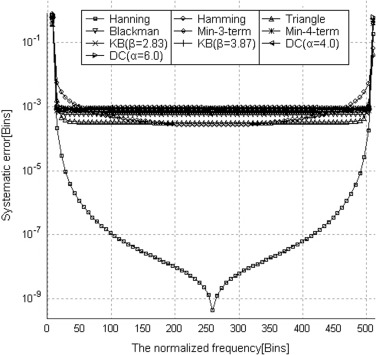
\includegraphics [scale=0.9] {picture7.png}
	\caption{SME предложенного алгоритма для разных окон.}
	\label{img:picture7}
\end{figure}

Исследование влияния шума

В этом пункте рассмотрим, что косинусоида (cosine-wave) была искажена аддитивным белым гауссовским шумом (white Gaussian noise) e(n)
с нулевым средним и дисперсией, соответствующей соотношению сигнал / шум (SNR – Signal-to-Noise Ratio) в диапазоне от $-5$ до $80$ дБ. Теоретическая частота была произвольно выбрана в интервале [255,5;256,5), чтобы минимизировать помехи от отрицательной частоты. Фазовое сканирование (Phase scanning) проводилось для каждой частоты, и в результате была выбрана наихудшая ситуация. В общей сложности $10000$ экземпляров таких тестовых сигналов были сгенерированы для каждого значения SNR, и была оценена среднеквадратичная ошибка (RMSE – root-mean-square error). На рисунке \ref{img:picture8} показана RMSE для разных окон в зависимости от SNR.

\begin{figure}[ht]
	\centering
	%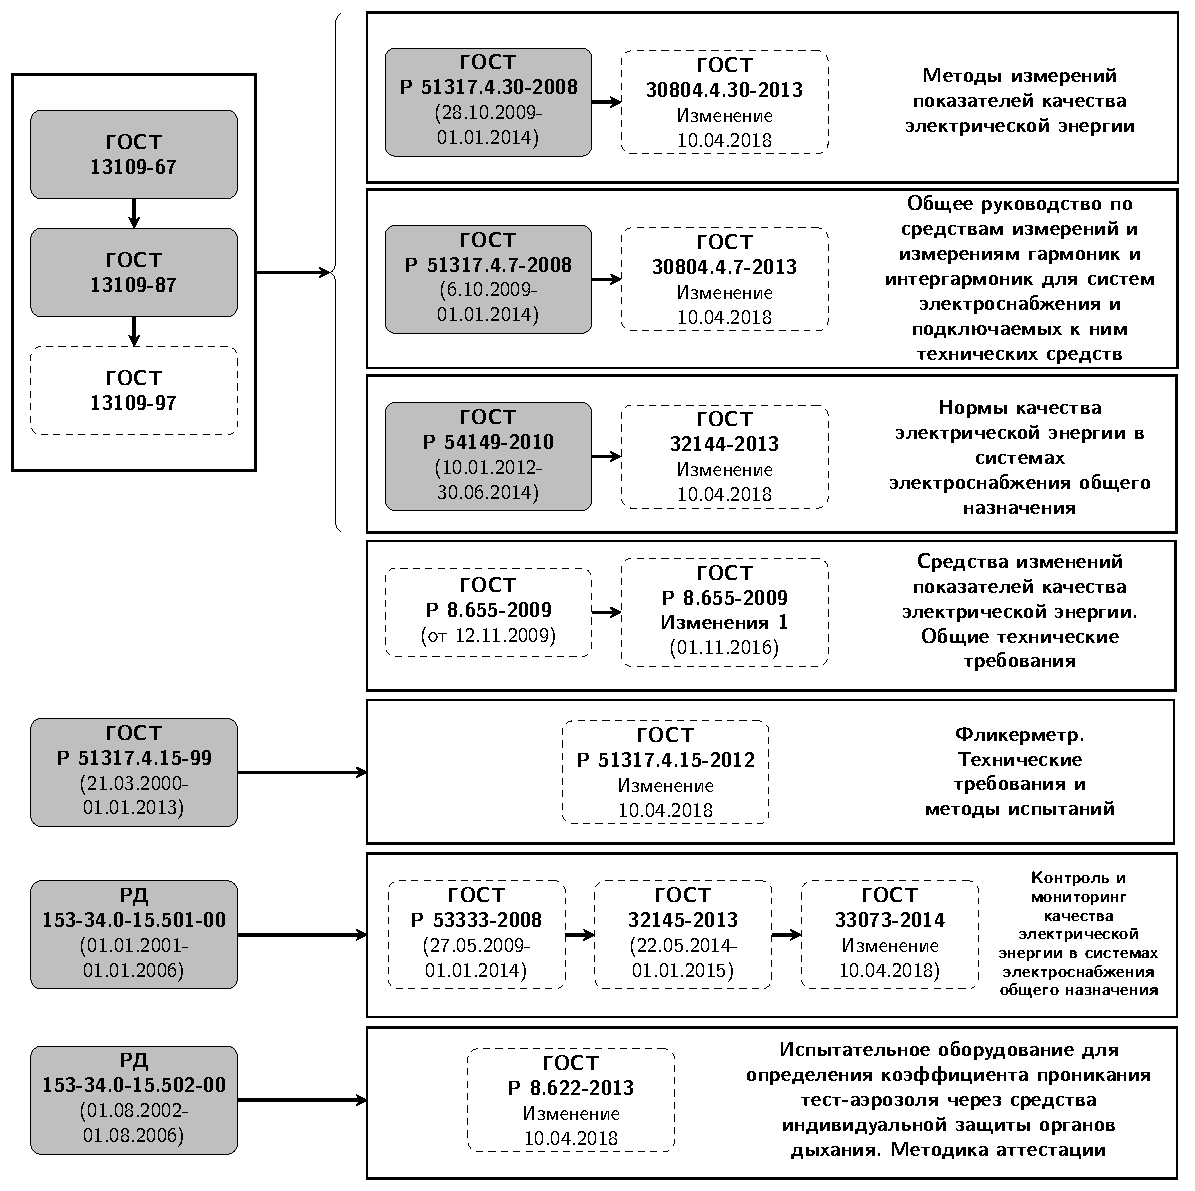
\includegraphics [scale=0.27] {picture1.png}
	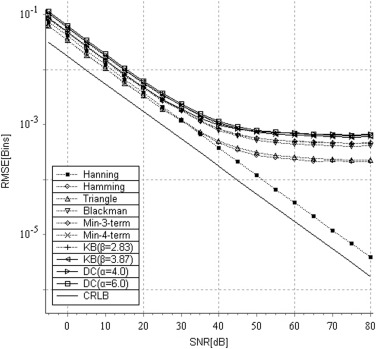
\includegraphics [scale=0.9] {picture8.png}
	\caption{RMSE предложенного алгоритма для разных окон.}
	\label{img:picture8}
\end{figure}

Нижняя граница Крамера–Рао (CRLB – Cramer–Rao lower bound) для оценки частоты также показана для сравнения. За $N\gg 1$ асимптотический CRLB оценки частоты в \labelcref{eq:equation12}  задается формулой [168]:

%[168.	Belega D., Dallet D. Multifrequency signal analysis by interpolated DFT method with maximum sidelobe decay windows //Measurement. – 2009. – Т. 42. – №. 3. – С. 420-426.]

\begin{equation}
\label{eq:equation61}
\sigma_{f} \approx \frac{6 f^2 _s}{{(2 \pi)^2}p N^3}
\end{equation}

где $p$ – SNR определяется как $\frac{A^2}{2 \ sigma ^2}$;
$\sigma^2$ – дисперсия белого гауссовского шума.

Можем четко наблюдать, что RMSE для окна Хеннинга является линейным во всем диапазоне SNR, потому что нет ошибок подгонки основного лепестка. В остальных случаях RMSE становится плоской из-за ошибок аппроксимации. На рисунке показано, что шум оказывает значительное влияние (significant impact) на неопределенность оценки при низком SNR. Таким образом, систематические ошибки можно почти игнорировать. Напротив, когда SNR высокое, систематические ошибки становятся основным источником ошибок. Значение отклонения SNR составляет около $30-40$ дБ, в зависимости от окна. Результаты также показывают, что когда SNR ниже перегиба, окна с узким основным лепестком (main-lobe) превосходят окна с широким основным лепестком. Это соответствует эквивалентной ширине полосы шума (ENBW – equivalent noise bandwidth), которая является эффективным индексом (effective index) для оценки свойств шума окна. 

\subsection{Сравнительное исследование} \label{sec:ch2/sec5_5}

В этом разделе некоторые симуляции предназначены для сравнения характеристик нового алгоритма (короткого как IpZPMF) с современными алгоритмами, включая алгоритм двухточечной интерполяции (interpolation) для окна Хеннинга (Hanning window), предложенного Грандке (Grandke) в $1983$ году [163] алгоритм трехточечной интерполяции для окна Хеннинга (Hanning window), предложенный Агрежем (Agrež) в $2002$ году [166], алгоритм интерполяции на основе 3-точечного модуля и трехточечный алгоритм интерполяции на основе сложного спектра (complex spectrum based interpolation algorithm), упомянутый Якобсеном (Jacobsen) и Коотсукосом (Kootsookos) в $2007$ году [167] полиномиальное приближение (polynomial approximation) с двумя и тремя точками Алгоритмы интерполяции, предложенные Дудой (Duda) в $2011$ году [170] и алгоритм интерполяции на основе 2-точечного сложного спектра, представленный Ченом (Chen) в $2008$ году. Параметры косинусоидальной волны (cosine wave), а также количество отсчетов и частота отсчетов (sampling frequency) такие же, как в предыдущем разделе.

% [163.-Grandke T. Interpolation algorithms for discrete Fourier transforms of weighted signals //IEEE transactions on instrumentation and measurement. – 1983. – Т. 32. – №. 2. – С. 350-355.]

%[166.-Agrez D. Weighted multipoint interpolated DFT to improve amplitude estimation of multifrequency signal //IEEE Transactions on Instrumentation and Measurement. – 2002. – Т. 51. – №. 2. – С. 287-292.]

%[167.-Jacobsen E., Kootsookos P. Fast, accurate frequency estimators [DSP Tips & Tricks] //IEEE Signal Processing Magazine. – 2007. – Т. 24. – №. 3. – С. 123-125.]

%[170.-Duda K. DFT interpolation algorithm for Kaiser–Bessel and Dolph–Chebyshev windows //IEEE Transactions on Instrumentation and Measurement. – 2011. – Т. 60. – №. 3. – С. 784-790.]

Без шума.

Чтобы оценить эффективность этих подходов для разных смещений по частоте, мы устанавливаем $\delta_\omega$ в диапазоне от $-0,5$ до $0,5$ с шагом $0.05$. Для каждого $\delta_\omega$ $72$ значения равноудалены в интервале $(-\pi,\pi]$ были выбраны для фазы косинусоидальной волны. Аналогичным образом, максимальное абсолютное значение между истинной и расчетной частотой было выбрано в качестве результата. На рисунке \ref{img:picture9} показаны частотные ошибки (frequency errors) для восьми методов коррекции (correction methods), когда выборки были взвешены окном Хеннинга (Hanning) до DFT. 

\begin{figure}[ht]
	\centering
	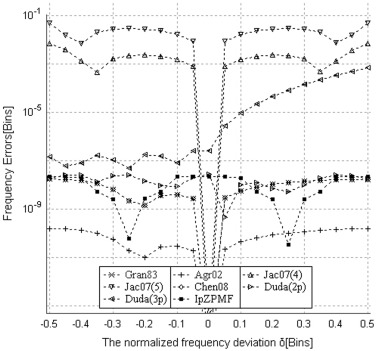
\includegraphics [scale=0.9] {picture9.png}
	\caption{Ошибки оценки частоты для окна Хеннинга.}
	\label{img:picture9}
\end{figure}

Методы могут оценивать частоту (estimate frequency) с относительно высокой точностью (high precision), за исключением – алгоритма интерполяции на основе $3$-точечного модуля, где максимальная погрешность частоты составляет около $10^ -2$, и трехточечный алгоритм интерполяции на основе сложного спектра, где максимальная погрешность частоты составляет около $10^ -1$. Наилучшим результатом является алгоритм трехточечной интерполяции для окна Хеннинга, где погрешность частоты составляет менее $10^ -9$. Предложенный алгоритм также дает очень маленькую ошибку около $10^-8$ результаты, в которых образцы, взвешенные в окне Хэмминга (Hamming window) и окно Блекмана (Blackman window) представлены на рисунках \ref{img:picture10} и \ref{img:picture11}. 

\begin{figure}[ht]
	\centering
	%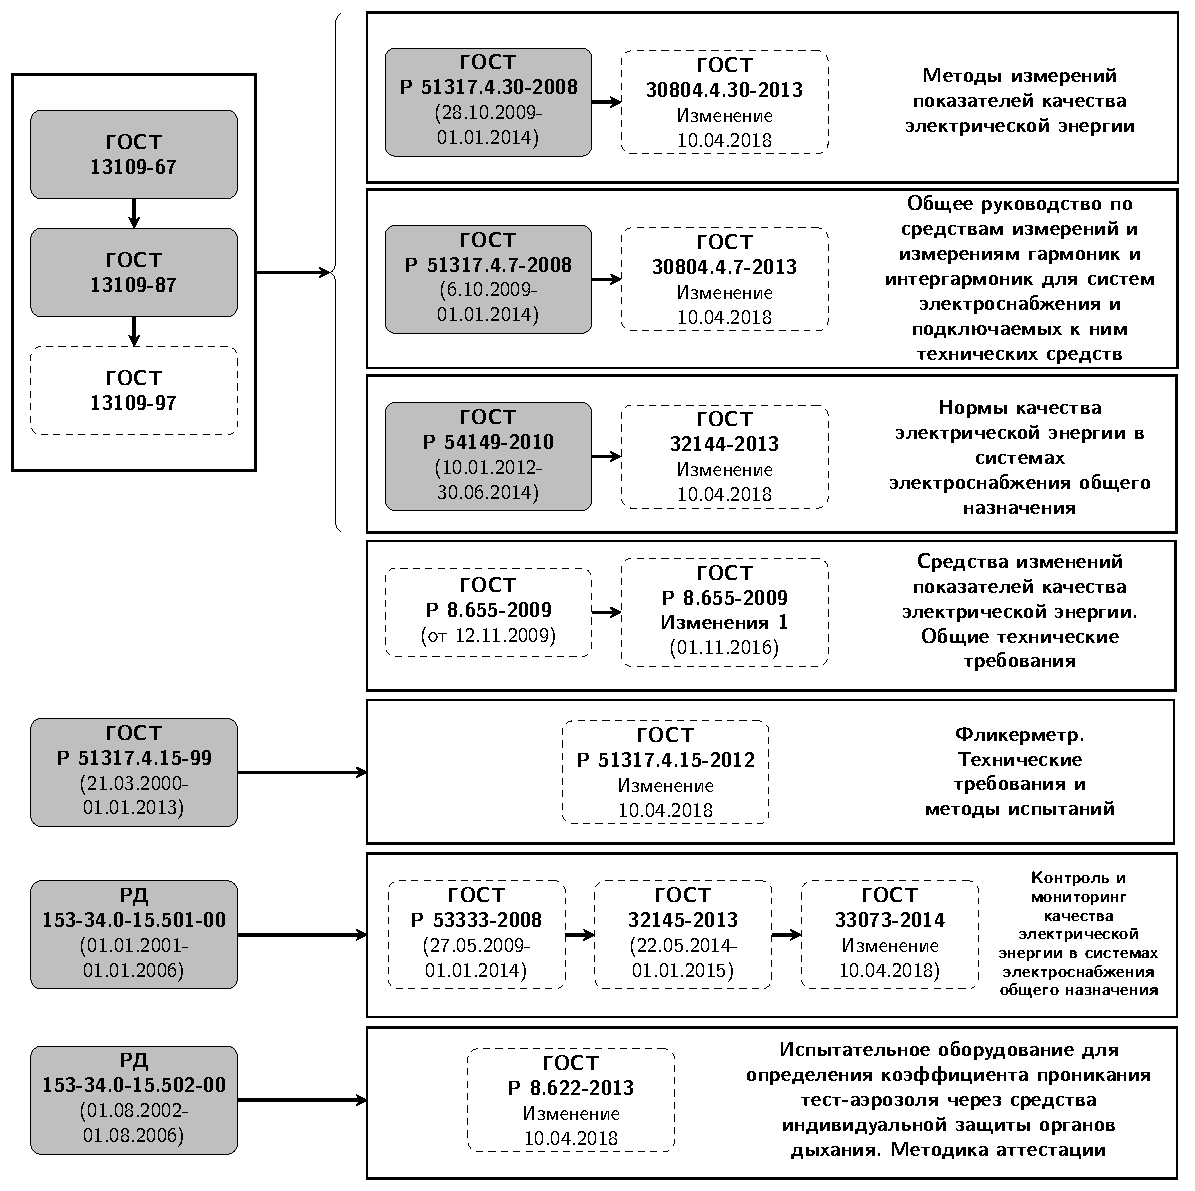
\includegraphics [scale=0.27] {picture1.png}
	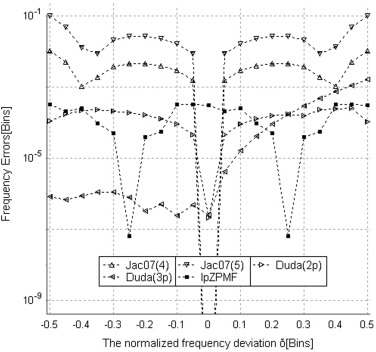
\includegraphics [scale=0.9] {picture10.png}
	\caption{Ошибки оценки частоты для окна Хэмминга.}
	\label{img:picture10}
\end{figure}

\begin{figure}[ht]
	\centering
	%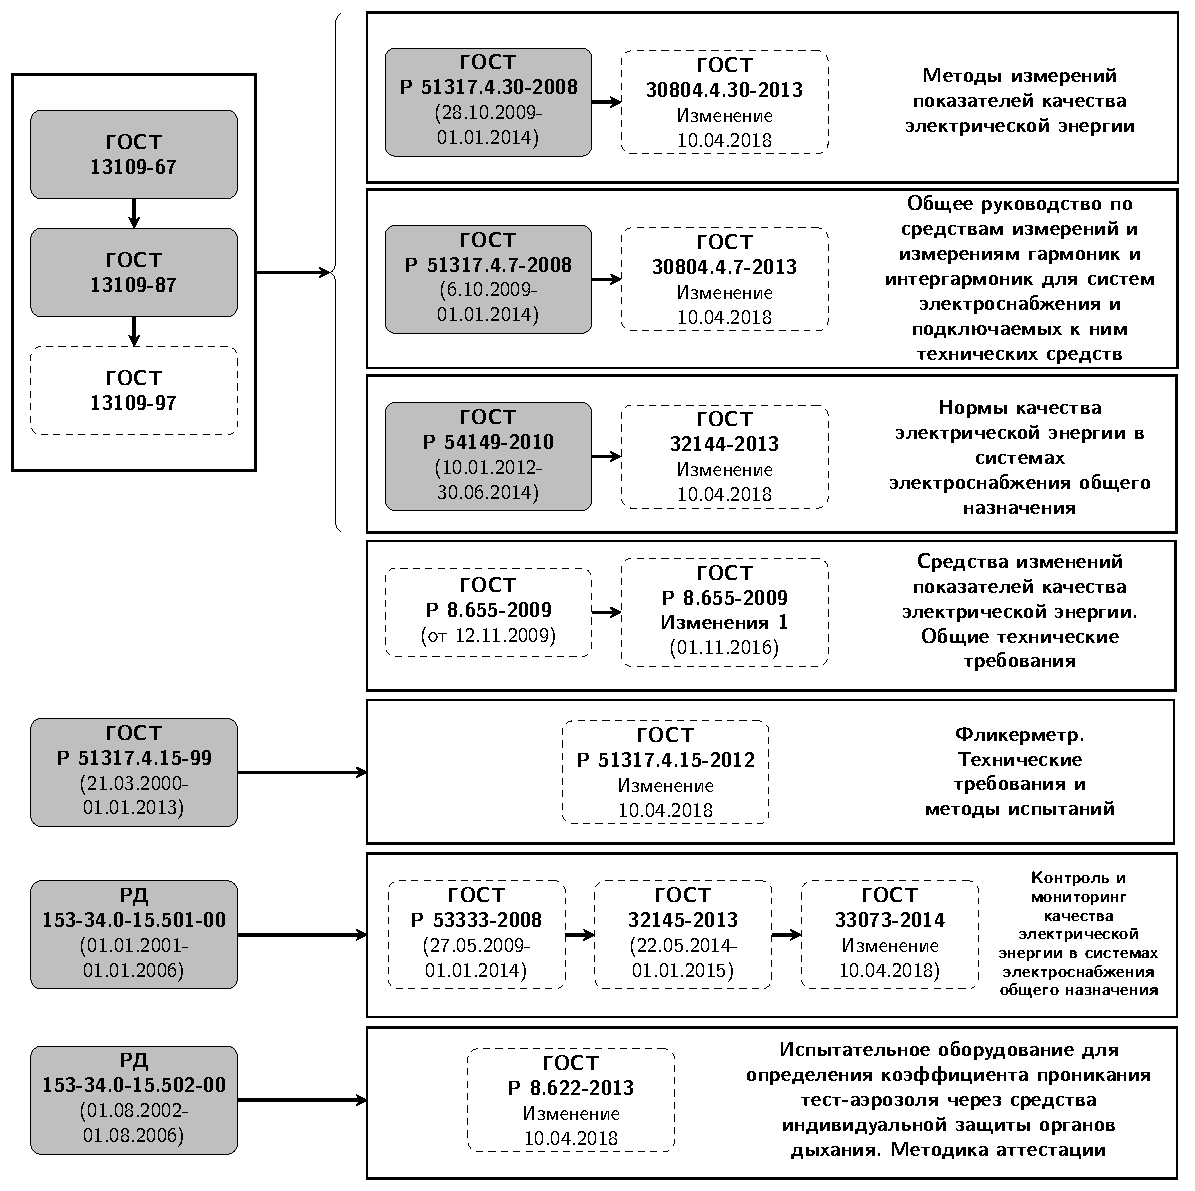
\includegraphics [scale=0.27] {picture1.png}
	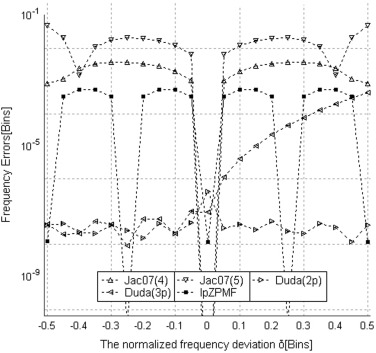
\includegraphics [scale=0.9] {picture11.png}
	\caption{Ошибки оценки частоты для окна Блэкмана.}
	\label{img:picture11}
\end{figure}

Поскольку алгоритм двухточечной интерполяции для окна Хеннинга, алгоритм трехточечной интерполяции для окна Хеннинга, алгоритм интерполяции на основе $2$-точечного сложного спектра совместимы только с окном Хеннинга (Hamming window), отображаются только результаты остальных пяти алгоритмов. Тенденции алгоритм интерполяции на основе $3$-точечного модуля и трехточечный алгоритм интерполяции на основе сложного спектра близки к тому, когда было принято окно Хеннинга (Hamming window). Алгоритмы интерполяции $2$-точечных и $3$-точечных полиномиальных приближений дают лучшие результаты, чем алгоритм интерполяции на основе $3$-точечного модуля и  трехточечный алгоритм интерполяции на основе сложного спектра. Как показано, IpZPMF очень стабилен, когда используются окна, отличные от Ханнинга, и обеспечивает максимальную погрешность частоты менее $10^ -3$. Результаты моделирования показывают, что в условиях отсутствия шума или низкого уровня шума и при использовании окна Хеннинга (Hamming window) алгоритм двухточечной интерполяции для окна Хеннинга, алгоритм трехточечной интерполяции для окна Хеннинга, алгоритм интерполяции на основе $2$-точечного сложного спектра являются приемлемыми вариантами, учитывая их высокую точность и простоту. Алгоритмы интерполяции полиномиальной аппроксимации и IpZPMF рекомендуются для других окон.

Устойчивость к аддитивному шуму.

Фактически, высокий уровень шума может даже привести к неправильному расположению правой спектральной линии (spectral line), даже если SNR выше порога. Эта проблема, называемая проблемой неправильной оценки полярности (polarity) (IPE – incorrect polarity estimation) в предыдущих ссылках [161], часто возникает при почти когерентном условии выборки $(|\delta_\omega|$ около нуля) для алгоритмов, основанных на $2$ точках, и при почти половине условие выборки периода $(|\delta_\omega |$ близко $0,5$) для алгоритмов, основанных на $3$ точках.

% [161.- Luo J., Xie M. Phase difference methods based on asymmetric windows //Mechanical Systems and Signal Processing. – 2015. – Т. 54. – С. 52-67]

Если спектральная линия выбрана неправильно, это не только влияет на значение $\delta_\omega$ но также приводит к изменению знака, что приводит к значительной ошибке в оценке частоты. Чтобы сравнить производительность (compare performance) различных алгоритмов с аддитивным шумом (additive noise), теоретические сигналы были получены с аддитивным нулевым Гауссовым шумом (Gaussian noise). SNR было установлено на $-5$ дБ, чтобы обеспечить высокую вероятность (high probability) неправильной оценки полярности. Частота сканировалась от $255,5$ Гц до $256,5$ Гц с шагом $0,025$ Гц, и случайная фаза была равномерно распределена на  $(-\pi,\pi]$ был принят. В общей сложности $50000$ независимых экземпляров (independent instances) были созданы для каждой частоты.

На рисунке \ref{img:picture12}, RMSE для окна Хеннинга (Hanning window) отображается как функция отклонения частоты $\lambda_{\omega}$. 

\begin{figure}[ht]
	\centering
	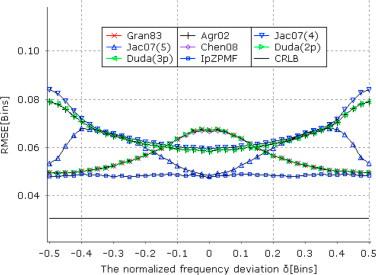
\includegraphics [scale=0.9] {picture12.png}
	\caption{RMSE различных алгоритмов для окна Хеннинга SNR=$-5$ dB.}
	\label{img:picture12}
\end{figure}

Здесь мы видим, что три двухточечных алгоритма (алгоритм двухточечной интерполяции для окна Хеннинга, алгоритм интерполяции на основе $2$-точечного сложного спектра, полиномиальное приближение с двумя точками алгоритмы интерполяции) имеют почти одинаковую производительность. Как мы и ожидали, с уменьшением |$\delta_{\omega}$|, RMSE этих трех алгоритмов возрастает. Самые высокие значения достигаются при условии когерентной выборки ($\delta_{\omega}=0$). 

Трехточечные алгоритмы (полиномиальное приближение с $3$-мя точками алгоритм интерполяции, алгоритм трехточечной интерполяции для окна Хеннинга) показывают схожую производительность, но остальные алгоритмы отличаются друг от друга. Полиномиальное приближение с $3$-мя точками алгоритм интерполяции, алгоритм трехточечной интерполяции для окна Хеннинга, алгоритм интерполяции на основе $3$-точечного модуля уменьшаются как |$\delta_{\omega}$| уменьшается и достигает минимума при $\delta_{\omega}=0$. Значения 
трехточечный алгоритм интерполяции на основе сложного спектра сначала увеличиваются, но затем постепенно снижаются до низкого уровня. Тенденции предлагаемого алгоритма относительно стабильны. Значения остаются на одном уровне с небольшими колебаниями. Более того, предлагаемый алгоритм имеет наименьшую среднеквадратичную величину во всем диапазоне $\delta_{\omega}$ по сравнению со всеми другими алгоритмами. Результаты для окна Хемминга (Hamming window) и окна Блэкмена (Blackman window) также показаны. Из рисунков \ref{img:picture13} и \ref{img:picture14} видно, что общие тенденции сходны с таковыми для окна Хеннинга (Hanning window).

\begin{figure}[ht]
	\centering
	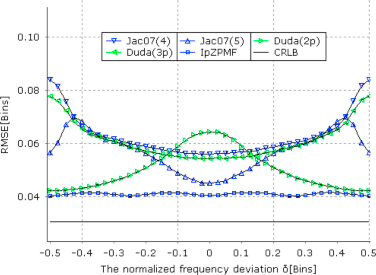
\includegraphics [scale=0.9] {picture13.png}
	\caption{RMSE различных алгоритмов для окна Хеннинга SNR=$-5$ dB.}
	\label{img:picture13}
\end{figure}

\begin{figure}[ht]
	\centering
	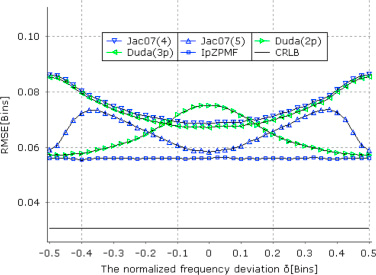
\includegraphics [scale=0.9] {picture14.png}
	\caption{RMSE различных алгоритмов для окна Блэкмена SNR=$-5$ dB.}
	\label{img:picture14}
\end{figure}

Результаты подтверждают тот факт, что IPE оказывает значительное влияние на текущие оценки (estimators) и что традиционные алгоритмы могут стать уязвимыми в присутствии шума. Предложенный алгоритм не только показывает сильную способность против IPE, но также имеет самый низкий RMSE. В результате он имеет подавляющее преимущество перед традиционными алгоритмами в условиях шума. Надежность может быть объяснена тем фактом, что спектральные линии, используемые в IpZPMF, намного сильнее, чем в традиционных алгоритмах. Кроме того, интервал спектральных линий, используемых в IpZPMF, составляет всего $\frac{1}{M}$ разрешения по частоте (frequency resolution). Это означает, что соседние спектральные линии могут содержать аналогичные шумы и, следовательно, обладают собственной способностью подавлять их часть. В традиционных алгоритмах, поскольку интервал между двумя спектральными линиями является частотным разрешением, корреляции шума резко ослабевают.

Был предложен алгоритм интерполяции (interpolation) для обеспечения точной оценки частоты. Описанный алгоритм основан на заполнении нулями и методах подгонки основного лепестка (main-lobe). Это легко понять, и обладает преимуществом практической простоты. Стоимость – это увеличение вычислений для БПФ (FFT). Новый алгоритм совместим с большинством классических окон, не требует знания спектра окна данных (data window) и не требует каких-либо предварительных расчетов. С помощью компьютерного моделирования (computer simulations) была продемонстрирована эффективность предложенного алгоритма для различных окон. Влияние систематической ошибки (systematic error) и белого Гауссового шума (white Gaussian noise) на точность частотных оценок (frequency estimations) также было изучено. Кроме того, обсуждалась проблема IPE в традиционных алгоритмах интерполяции. Результаты моделирования показывают, что предлагаемый алгоритм обладает внутренней устойчивостью к IPE и более высокой устойчивостью к аддитивному шуму (additive noise), чем предыдущие алгоритмы интерполяции.

Согласно определению в уравнениях \labelcref{eq:equation31} и \labelcref{eq:equation32}, имеем

\begin{equation}
\label{eq:equation62}
\gamma_1 = \frac{\left| X(l-1)\right|}{\left| X(l)\right|} = \frac{\sin \pi({\delta + \varepsilon})}{\sin \pi \delta} \cdot \frac{h(\delta)}{h(\delta + \varepsilon)}
\end{equation}

\begin{equation}
\label{eq:equation63}
\gamma_2 = \frac{\left| X(l+1)\right|}{\left| X(l)\right|} = \frac{\sin \pi({\delta - \varepsilon})}{\sin \pi \delta} \cdot \frac{h(\delta)}{h(\delta - \varepsilon)}
\end{equation}

\begin{equation}
\label{eq:equation64}
\gamma = \frac{\left| X(l+1)\right|}{\left| X(l-1)\right|} = \frac{\sin \pi({\delta - \varepsilon})}{\sin \pi ({\delta + \varepsilon})} \cdot \frac{h({\delta + \varepsilon})}{h(\delta - \varepsilon)}
\end{equation}

Знаем $\gamma_1$, является монотонно убывающей функцией и $\gamma_2$, $\gamma$ является монотонно возрастающей функцией в зависимости от $\delta$ в диапазоне $[-0.5;0.5]$. Итак, можем получить

\begin{equation}
\label{eq:equation65}
\gamma_{1 max} = \gamma_1 (\delta = - 0,5) = \frac{3 \cos \pi \varepsilon}{(1 + 2 \varepsilon)(1 - 2 \varepsilon)(3 - 2 \varepsilon)}
\end{equation}

\begin{equation}
\label{eq:equation66}
\gamma_{1 min} = \gamma_1 (\delta = 0,5) = \frac{3 \cos \pi \varepsilon}{(1 + 2 \varepsilon)(1 - 2 \varepsilon)(3 + 2 \varepsilon)}
\end{equation}

\begin{equation}
\label{eq:equation67}
\gamma_{2 max} = \gamma_2 (\delta = 0,5) = \frac{3 \cos \pi \varepsilon}{(1 + 2 \varepsilon)(1 - 2 \varepsilon)(3 - 2 \varepsilon)}
\end{equation}

\begin{equation}
\label{eq:equation68}
\gamma_{2 min} = \gamma_2 (\delta = -0,5) = \frac{3 \cos \pi \varepsilon}{(1 + 2 \varepsilon)(1 - 2 \varepsilon)(3 + 2 \varepsilon)}
\end{equation}

\begin{equation}
\label{eq:equation69}
\gamma_{max} = \gamma(\delta = 0,5) = \frac{1,5+ \varepsilon}{1,5 - \varepsilon}
\end{equation}

\begin{equation}
\label{eq:equation70}
\gamma_{min} = \gamma(\delta = -0,5) = \frac{1,5 - \varepsilon}{1,5 + \varepsilon}
\end{equation}

Согласно бесконечному представлению Эйлера функции синуса:

\begin{equation}
	\label{eq:equation71}
	\sin \pi \delta = \pi \delta \prod\limits_{n = 1}^\infty \left( 1- \frac{\delta^2}{n^2} \right) 
\end{equation}

\begin{equation}
\label{eq:equation72}
E(\delta) = \frac{\sin(\pi \delta) }{h(\delta)} = \frac{\pi \delta \prod\limits_{n = 1}^\infty \left( 1- \frac{\delta^2}{n^2}\right)}{\pi \delta (1 - \delta^2)} = \prod\limits_{n = 2}^\infty \left( 1 - \frac{\delta^2}{n^2}\right) \geq 0 
\end{equation}

Находим производную $E(\delta)$:     

\begin{equation}
\label{eq:equation73}
E'(\delta) = E(\delta)L(\delta)
\end{equation}

\begin{equation}
\label{eq:equation74}
L(\delta) = \sum_{n=2}^{\infty} \frac{-2 \delta}{n^2 - \delta^2} = \sum_{n=2}^{\infty} \left(  \frac{1}{n + \delta} -  \frac{1}{n - \delta} \right) 
\end{equation}

\begin{equation}
\label{eq:equation75}
D(\delta) = \frac{E(\delta)}{E(\delta + \epsilon)} = \frac{\prod\limits_{n = 2}^\infty \left( 1 - \frac{\delta^2}{n^2} \right) }{\prod\limits_{n = 2}^\infty \left( \frac{1 - (\delta + \epsilon)^2}{n^2}\right)} = \prod\limits_{n = 2}^\infty \frac{n^2 - \delta^2}{n^2 - (\delta + \epsilon)^2}
\end{equation}

\begin{equation}
\label{eq:equation76}
D'(\delta) = \frac{E(\delta)L(\delta)E(\delta + \epsilon) - E(\delta)E(\delta + \epsilon)L(\delta + \epsilon)}{E^2 (\delta + \epsilon)} = \frac{E(\delta) [L(\delta) - L(\delta + \epsilon)])}{E(\delta + \epsilon)}
\end{equation}

\begin{equation}
\label{eq:equation77}
L(\delta) - L(\delta + \epsilon) = \sum_{n=2}^{\infty} \left(  \frac{\epsilon}{(n + \delta)(n + \delta + \epsilon)} + \frac{\epsilon}{(n - \delta)(n - \delta - \epsilon)} \right) > 0
\end{equation}

\begin{equation}
\label{eq:equation78}
D'(\delta) > 0 
\end{equation}

$D(\delta)$ -- монотонно возрастающая функция в зависимости от $\delta$, $\frac{1}{D(\delta)}$ -- монотонно убывающая функция. 

На основании уравнения \labelcref{eq:equation72} $\gamma_1, \gamma_2$ могут быть представлены:

\begin{equation}
\label{eq:equation79}
\gamma_1 = \frac{E(\delta + \epsilon)}{E(\delta)} 
\end{equation}

\begin{equation}
\label{eq:equation80}
\gamma_2 = \frac{E(\delta - \epsilon)}{E(\delta)} 
\end{equation}

\begin{equation}
\label{eq:equation81}
p(\delta) = \frac{[E(\delta + \epsilon)(3 + 2 \epsilon) + E(\delta - \epsilon)(3 - 2 \epsilon)]}{E(\delta)}
\end{equation}

\begin{equation}
\label{eq:equation82}
q(\delta) = \frac{[E(\delta + \epsilon)(3 - 2 \epsilon) + E(\delta - \epsilon)(3 + 2 \epsilon)]}{E(\delta)}
\end{equation}

\begin{equation}
\label{eq:equation83}
p'(\delta) = \frac{H_{p}(\delta, \epsilon)}{E(\delta)}
\end{equation}

\begin{equation}
\label{eq:equation84}
q'(\delta) = \frac{H_{q}(\delta, \epsilon)}{E(\delta)}
\end{equation}

Где $H_{p}(\delta, \epsilon)$ и $H_{q}(\delta, \epsilon)$ соответственно:

\begin{equation}
\label{eq:equation85}
H_{p}(\delta, \epsilon) = E(\delta + \epsilon)(3 + 2 \epsilon) [L (\delta + \epsilon) - L(\delta)] + E(\delta - \epsilon)(3 - 2\epsilon) [L(\delta - \epsilon) - L(\delta)]
\end{equation}

\begin{equation}
\label{eq:equation86}
H_{q}(\delta, \epsilon) = E(\delta + \epsilon)(3 - 2 \epsilon) [L (\delta + \epsilon) - L(\delta)] + E(\delta - \epsilon)(3 + 2\epsilon)[L(\delta - \epsilon) - L(\delta)]
\end{equation}

\begin{equation}
\label{eq:equation87}
H_{p}(\delta, \epsilon) + H_{p}(- \delta, \epsilon) = 4 \epsilon E (\delta + \epsilon) [L(\delta + \epsilon) - L(\delta)] + 4 \epsilon E (\delta - \epsilon)[L(\delta) - L (\delta - \epsilon)] 
\end{equation}

\begin{equation}
\label{eq:equation88}
H_{q}(\delta, \epsilon) + H_{q}(- \delta, \epsilon) = - 4 \epsilon E (\delta + \epsilon) [L(\delta + \epsilon) - L(\delta)] - 4 \epsilon E (\delta - \epsilon)[L(\delta) - L (\delta - \epsilon)]  
\end{equation}

Если $L (\delta - \epsilon) - L(\delta) < 0$ и $L(\delta) - L(\delta - \epsilon) < 0$, то:

\begin{equation}
\label{eq:equation89}
H_{p}(\delta, \epsilon) + H_{p}(- \delta, \epsilon) < 0  
\end{equation}

\begin{equation}
\label{eq:equation90}
H_{q}(\delta, \epsilon) + H_{q}(- \delta, \epsilon) > 0  
\end{equation}

\begin{equation}
\label{eq:equation91}
H_{p}(\delta, \epsilon) < 0
\end{equation}

\begin{equation}
\label{eq:equation92}
H_{q}(\delta, \epsilon) > 0
\end{equation}

\begin{equation}
\label{eq:equation93}
p'(\delta) = \frac{H_{p}(\delta, \epsilon)}{E(\delta)} < 0
\end{equation}

\begin{equation}
\label{eq:equation94}
q'(\delta) = \frac{H_{q}(\delta, \epsilon)}{E(\delta)} > 0
\end{equation}

где $p(\delta)$ -- убывающая функция;

$\delta$ -- убывающая функция;

$q(\delta)$ -- возрастающая функция.

\begin{equation}
\label{eq:equation95}
I(\delta, \epsilon) = \frac{E(\delta - \epsilon)}{E(\delta + \epsilon)} \cdot \frac{L(\delta - \epsilon) - L(\delta)}{L(\delta) - L(\delta + \epsilon)}
\end{equation}

\begin{equation}
\label{eq:equation96}
K(\epsilon) = \frac{3 + 2\epsilon}{3 - 2\epsilon}
\end{equation}

Если $I(\delta, \epsilon) > 0$, $0 < K(\epsilon) < 1 < K (\epsilon)$, а также $K(- \epsilon)K(\epsilon) = 1$.

\begin{equation}
\label{eq:equation97}
\frac{H_{p}(\delta, \epsilon)}{H_{p}(- \delta, \epsilon)} = \frac{I(\delta, \epsilon) - K(\epsilon)}{K(- \epsilon) - I(\delta, \epsilon)}
\end{equation}
 
\begin{equation}
\label{eq:equation98}
\frac{H_{q}(\delta, \epsilon)}{H_{q}(- \delta, \epsilon)} = \frac{K(- \epsilon) -  I(\delta, \epsilon)}{I(\delta, \epsilon) - K(\epsilon)}
\end{equation}

Если $\delta > 0$, то:
\begin{equation}
\label{eq:equation99}
K(- \epsilon) < \frac{E(\delta + \epsilon)}{E(\delta - \epsilon)}
\end{equation}

\begin{equation}
\label{eq:equation100}
1 < \frac{L(\delta) - L(\delta + \epsilon)}{L(\delta - \epsilon) - L(\delta)} < K(\epsilon)
\end{equation}

\begin{equation}
\label{eq:equation101}
K(- \epsilon) < I(\delta, \epsilon) < K(\epsilon)
\end{equation}

Подставив уравнение \labelcref{eq:equation101} в  \labelcref{eq:equation97} и  \labelcref{eq:equation98}, то $\frac{H_{p}(\delta, \epsilon)}{H_{p}(- \delta, \epsilon)} > 0$, а также $\frac{H_{q}(\delta, \epsilon)}{H_{q}(- \delta, \epsilon)} > 0$

\begin{equation}
\label{eq:equation102}
T(\delta,  \epsilon) = \frac{L(\delta) - L(\delta + \epsilon)}{L(\delta - \epsilon) - L(\delta)} \cdot \frac{ \sum_{n = 2}^{\infty} a_{n}}{\sum_{n = 2}^{\infty} b_{n}}
\end{equation}

\begin{equation}
\label{eq:equation103}
a_{n} = \frac{1}{(n + \delta)(n + \delta - \epsilon)} + \frac{1}{(n - \delta)(n - \delta - \epsilon)} 
\end{equation}

\begin{equation}
\label{eq:equation104}
b_{n} = \frac{1}{(n + \delta)(n + \delta - \epsilon)} + \frac{1}{(n - \delta)(n - \delta + \epsilon)} 
\end{equation}

\begin{equation}
\label{eq:equation105}
C_{n} = \frac{a_{n}}{b_{n}} = \frac{n^2 -\delta^2 - \epsilon^2 + 2\delta \epsilon}{n^2 -\delta^2 - \epsilon^2 - 2\delta \epsilon} \cdot \frac{n^2 + \delta^2 + \delta \epsilon}{n^2 + \delta^2 - \delta \epsilon}
\end{equation}

Если $\delta > 0$, $\frac{n^2 - \delta^2 - \epsilon^2 +2\delta \epsilon}{n^2 - \delta^2 - \epsilon^2 - 2\delta \epsilon} > 1$ также $\frac{n^2 + \delta^2 + \delta \epsilon}{n^2 + \delta^2 - \delta \epsilon} > 1$, то:

\begin{equation}
\label{eq:equation106}
C_{n} > C_{n + 1} > 1 
\end{equation}

\begin{equation}
\label{eq:equation107}
1 < T(\delta, \epsilon) < C_{2}
\end{equation} 

$C_{n}$ может быть записана:
\begin{equation}
\label{eq:equation108}
C = \frac{1 + \frac{2 \delta \epsilon}{(n^2 - \delta^2 - \epsilon^2)}}{1 - \frac{2 \delta \epsilon}{(n^2 - \delta^2 - \epsilon^2)}} \cdot \frac{1 + \frac{\delta \epsilon}{(n^2 + \delta^2)}}{1 - \frac{\delta \epsilon}{(n^2 + \delta^2)}}
\end{equation} 

Вводя параметр $D_{1} =  \frac{2 \delta \epsilon}{(n^2 - \delta^2 - \epsilon^2)}$ и $D_{1} =  \frac{\delta \epsilon}{n^2 + \delta^2}$

\begin{equation}
\label{eq:equation109}
C_{n} = \frac{1 + D_{1}}{1 - D_{1}} \cdot  \frac{1 + D_{2}}{1 - D_{2}} = \frac{1 + D_{1}D_{2} + D_{1} + D_{2}}{1 + D_{1}D_{2} - D_{1} - D_{2}} = \frac{1 + \frac{(D_{1} + D_{1})}{(1 + D_{1}D_{2})}}{1 - \frac{(D_{1} + D_{1})}{(1 + D_{1}D_{2})}}
\end{equation} 

\begin{equation}
\label{eq:equation110}
D = \delta \epsilon \frac{3n^2 - \epsilon^2 + \delta^2}{(n^2 - \delta^2 - \epsilon ^2)(n^2 + \delta ^2) + 2 \delta ^2 \epsilon^2} < \delta \epsilon \frac{3 n^2 + \frac{1}{4}}{(n^2 - \frac{1}{2})n^2}
\end{equation} 

Если $n = 2$, то
\begin{equation}
\label{eq:equation111}
D < \epsilon \ frac{6 + \frac{1}{8}}{14} < \frac{2}{3} \epsilon
\end{equation} 

Соответственно:
\begin{equation}
\label{eq:equation112}
1 < T(\delta, \epsilon) < C_{2} < \frac{1 + \frac{2 \epsilon}{3}}{1 - \frac{2 \epsilon}{3}} = K(\epsilon)
\end{equation} 

При $\delta <0$ получаем $K(\epsilon) < T(\delta, \epsilon) < 1$ 

\section{Оценка частоты энергосистемы с использованием дифференциатора наименьших средних квадратов} \label{sec:ch2/sec6}

Частота энергосистемы является решающим фактором для мониторинга и контроля рабочего состояния сети, а также для синхронизации и управления электронными преобразователями мощности, подключенными к ней. Некоторые методы синхронизации, используемые в преобразователях мощности, подключенных к сети, основаны на точной оценке частоты сети. 
\cite{lee2013novel, lee2011active}. Несколько методов было разработано для получения частоты электросети, как описано в \cite{chen2013comparative}. На основе DFT \cite{borkowski2014interpolated,kamwa2004performance}, искусственная нейронная сеть \cite{jiang2014frequency}, частотно-замкнутый контур (FLL) \cite{fedele2014frequency}, широколинейная фаза наименьшего среднего значения (WLLMP) \cite{xia2014widely}, наименьшие квадраты (LS) \cite{kuvsljevic2013ls}, Комплексные наименьшие средние квадраты \cite{pradhan2005power, xia2014complex} наименьшие квадраты, примененные к фазовому углу \cite{ramos2015frequency}, улучшенный алгоритм рекурсивного ньютоновского типа (IRNTA) \cite{ray2015improved}, фильтр Калмана \cite{routray2002novel}, Prony \cite{rubeena2014accurate}, улучшенная фазовая автоподстройка частоты (EPLL) ) \cite{karimi2010application}, фаза кадра синхронной автоподстройки частоты (ОСР-ФАПЧ) \cite{golestan2013performance}, и переход через нуль \cite{ramos2005synchronizing} среди доступных методов оценки частоты.
Точность оценки частоты сильно зависит от помех в энергосистеме. Нарушения могут быть разделены на две основные группы: стационарное состояние и переходные процессы. Проблемы установившегося состояния включают несбалансированные напряжения, гармоники, низкочастотные колебания амплитуды и отклонения частоты. Временные проблемы включают в себя внезапные изменения основной формы волны напряжения и амплитуд и фаз гармоник, изменения частоты, скачки фазового угла, пики, вырезы, экспоненциальные затухающие компоненты и шум. Поскольку возмущения энергосистемы увеличиваются с распространением систем распределенной генерации и нелинейных нагрузок, крайне важно, чтобы алгоритм оценки частоты был невосприимчив к помехам. Одновременно алгоритм должен иметь достаточную пропускную способность для отслеживания изменений частоты. Компромисс между шириной полосы и отклонением помех является общим свойством для всех методов оценки частоты.
В этой статье предлагается метод оценки частоты, основанный на дифференцировании фазового угла комплексной синусоиды, полученной путем применения матрицы преобразования Кларка к напряжениям сетки. Насколько известно авторам, первые случаи использования фазовых углов для получения частоты сложной синусоиды были описаны Треттером \cite{tretter1985estimating} и Кейем \cite{kay1989fast}. МакКиллиам \cite{mckilliam2010frequency} предложил версию, более устойчивую к шуму за счет времени вычислений. Идея в \cite{tretter1985estimating} состоит в том, чтобы использовать метод наименьших квадратов (LSM), чтобы развернуть развернутый фазовый угол в прямую линию, где наклон указывает частоту. Таким образом, частота задается первой производной фаTзового угла. Таким образом, \cite{tretter1985estimating} дает те же результаты, что и применение фильтра Савицкого – Голея первого порядка \cite{schafer2011savitzky} к фазовым углам. Версия Kay \cite{kay1989fast} улучшает оценку, избегая шага разворачивания фазового угла, используя разности фазного угла назад. Другое тонкое улучшение заключается в том, что в версии Kay нет ограничения на то, что количество выборок должно быть нечетным. Вклад этой статьи: добавление фильтра скользящего среднего (MAF) для дальнейшего сглаживания оценки частоты и обеспечения полной оценки устойчивости оценщика к гармоникам напряжения и дисбалансам; разработка метода выбора количества выборок, используемых алгоритмом LMS; рекурсивная реализация алгоритма LMS.

\subsection{Оценка частоты сетки с использованием фазовых углов и алгоритма LMS} \label{sec:ch2/sec1_1}

Используя преобразование Кларка, сеточные напряжения выражаются в стационарном $\alpha \beta$ -- кадре :

\begin{equation}
\label{eq:equation113}
[u_{\alpha}[n],u_{\beta}[n]]^T=\dfrac{\sqrt{2}}{2\sqrt{3}} 
\begin{bmatrix}
2 & -1 & -1\\
0 & \sqrt{3} & -\sqrt{3}
\end{bmatrix}
[u_1[n], u_2[n], u_3[n]]^T ,
\end{equation} 

где $u_1[n], u_2[n]$  и  $u_3[n]$ представляют текущую выборку трех фазно-нейтральных напряжений сетки, выбранных на частоте $f_s$  и периоде $T_s$.
Затем компоненты $u_{\alpha}[n] , u_{\beta}[n]$ используются для формирования сложной синусоиды $u_c[n]$:
 
\begin{equation}\label{eq:equation114}
u_c [n]= u_{\alpha}[n]+j* u_{\beta}[n] ,
\end{equation}

который также может быть представлен в полярной форме:

\begin{equation}\label{eq:equation115}
u_c [n]= a[n]exp(j\theta [n] ),
\end{equation}

где фазовый угол $\theta [n]$ получается выражением:

\begin{equation}\label{eq:equation116}
\theta[n]=atan (u_{\beta} [n],u_{\alpha}[n] ),
\end{equation}

и $ atan(y,x)$  функция представляет угол четырех квадрантов из функции $tan^{-1} \dfrac{x}{y}$

В незагрязненной сетке текущее значение фазового угла, определяемое как (4), равно фазовому углу основной положительной последовательности $(\theta^{1+})$, и текущая частота сетки        $(f_g [n])$ получается из разности между текущей и последней выборками фазового угла:

\begin{equation}\label{eq:equation117}
f_{g} [n]=(\theta[n]- \theta[n-1] ) f_{s} /(2\pi)
\end{equation}

В общей сетке, нарушенной гармониками, дисбалансами и шумом, фазовый угол $\theta$ является основным фазовым углом прямой последовательности $\theta ^{1+}$, на который накладывается фазовый угол ошибки. Значения $\theta ^{1+}$,  можно оценить, поместив развернутую последовательность $N$ элементов  $\theta`$ из значений $\theta$ в прямую линию. Расчетная частота сетки затем получается по наклону линии подгонки. Если метод наименьших квадратов используется для подгонки развернутых значений $\theta`$, текущий оцененный фазовый угол прямой последовательности $\theta ^{1+} [n]$  и текущая расчетная частота  $f_{g} [n] $  определяются как \cite{tretter1985estimating, kay1989fast}:

\begin{equation}\label{eq:equation118}
\hat{\theta}^{1+}[n] = \dfrac{6}{N(N+1)} \sum\limits_{i=0}^{N-1} i \theta^\prime[n+i-N+1]-\dfrac{2N-4}{N(N+1)} \sum\limits_{i=0}^{N-1} \theta^\prime[n+i-N+1]
\end{equation}

\begin{equation}\label{eq:equation119}
\hat f_{g}[n] = \dfrac{6f_{s}}{N(N^{2}+1)\pi} \sum\limits_{i=0}^{N-1} i \theta^\prime[n+i-N+1]-\dfrac{3f_{s}}{N(N+1\pi)} \sum\limits_{i=0}^{N-1} \theta^\prime[n+i-N+1]
\end{equation}

Последовательность $\theta^\prime [n+i-N+1], i = {0,1,…,N-1}$ получается путем развертывания последовательности $h$ фазового угла, образованной текущим значением $(i=0)$ и $N-1$ прошлыми элементами.

Чтобы избежать трудоемкой операции развертывания фазового угла, оценка частоты сетки 
\^f$_{g}$ может быть выражена в функции обратной разности $(\theta)$ фазового угла $(\delta)$, определяемой как:

\begin{equation}\label{eq:equation120}
\delta[n]  =
\begin{cases}
\theta[n]-\theta[n-1]-2\pi, &\text{если $\theta[n]-\theta[n-1] >\pi$} \\
\theta[n]-\theta[n-1], &\text{если $ -\pi<\theta[n]-\theta[n-1] \leqslant \pi$} \\
\theta[n]-\theta[n-1]+2\pi, &\text{если $\theta[n]-\theta[n-1] \leqslant -\pi$} 
\end{cases}
\end{equation}

\begin{figure}[ht]
	\centering
	%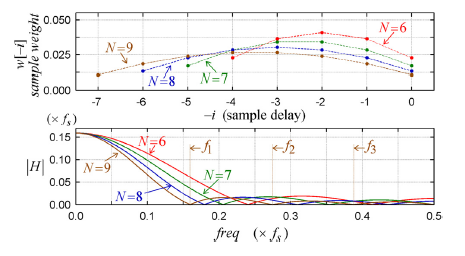
\includegraphics [scale=0.9] {f1.png}
	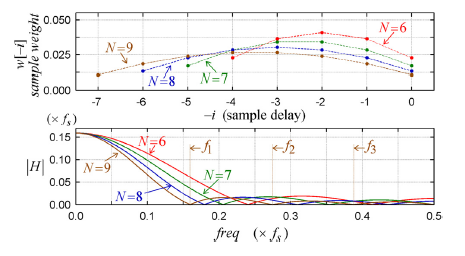
\includegraphics [width=0.9\linewidth] {f1.png}
	\caption{Оценщик (9) веса и амплитуды частотной характеристики образца.}
	\label{img:picture15}
\end{figure}

Три случая для вычисления $\delta$ необходимы для учета циклического характера фазового угла. Это позволяет избежать абсолютных разностей фазового угла, превышающих $\pi$ радиан.

Используя \labelcref{eq:equation120}, оценка частоты сетки \labelcref{eq:equation119} выражается как:

\begin{equation}\label{eq:equation121}
\hat f_{g}[n] = \sum\limits_{i=0}^{N+2} \dfrac{3f_{s}}{4\pi} 
\dfrac{N^2-4(i-\dfrac{1}{2}N +1)^{2}} {N(N^2 -1)} \delta[n-i] = \sum\limits_{i=0}^{N+2} f_s w [-i]\delta [n-i]
\end{equation}

где $w[-i]$ представляет вес выборки окна, примененный к каждой разности фаз и углов, задержанной на $i$ выборок$ (\delta [n - 1])$:

\begin{equation}\label{eq:equation122}
w[-i] =\dfrac{3}{4\pi} \dfrac{N^2-4(i-\dfrac{1}{2}N +1)^{2}} {N(N^2 -1)}, i=2-N, ..., -1, 0
\end{equation}

На \labelcref{img:picture15}  показан вес выборки окна \labelcref{eq:equation122} и частотная характеристика выражения \labelcref{eq:equation121} для четырех значений $ N $. Без потери общности и по соображениям ясности был выбран диапазон небольших значений $ N $. Частоты $ f_1, f_2 и f_3 $ являются частотами, для которых частотная характеристика имеет нулевое усиление для $ N = 9 $.

Как уже упоминалось в \cite{kay1989fast}, \labelcref{eq:equation121} достигает Крамера-Рао для сигнала к шуму (SNR) больше, чем на 6 дБ. Это означает, что этот оценщик будет иметь лучшее подавление шума для SNR более 6 дБ. Однако этот оценщик не может полностью отклонить содержание гармоник сетки, потому что нет значения N, которое приводит к нулевому усилению на всех частотах $ f=hf_g $, где $  h $ - порядок гармоник.

\subsection{Фильтрация оценки частоты с помощью фильтра скользящих средних} \label{sec:ch2/sec1_2}

В общей сетке, нарушенной гармониками и дисбалансами, выражение фазового угла $ \theta $ не имеет простой замкнутой формы, как в \labelcref{eq:equation116}. Тем не менее, следующие свойства подтверждаются численным моделированием: компонент постоянного тока создает колебание фазового угла с той же частотой, что и сетка; положительная последовательность гармоники n-го порядка дает осцилляцию ошибки фазового угла $ (n - 1) $, умноженную на частоту сетки; отрицательная последовательность гармоники n-го порядка создает осцилляцию ошибки фазового угла $ (n + 1) $, умноженную на частоту сетки; значение ошибки фазового угла в течение периода сетки равно нулю. На \labelcref{img:picture16} показаны четыре примера с различными условиями сетки, где $  \theta^{1+} $- это фазовый угол основной прямой последовательности, а $ \theta $- фазовый угол, полученный из \labelcref{eq:equation116}.

Фильтр скользящего среднего, применяемый к оценке частоты LMS $ ({\hat{f}}_g) $, может полностью устранить ошибки частоты из-за гармоник и дисбалансов, если длина фильтра совпадает с периодом сетки. Это происходит потому, что фильтр MAF определяется:

\begin{equation}\label{eq:equation123}
y[n] =\dfrac{1}{N} \sum\limits_{i=0}^{N-1} x [n-i]
\end{equation}

\begin{figure}[ht]
	\centering
	%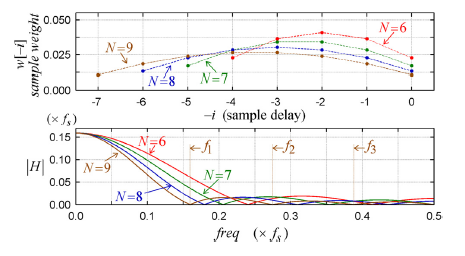
\includegraphics [scale=0.9] {f1.png}
	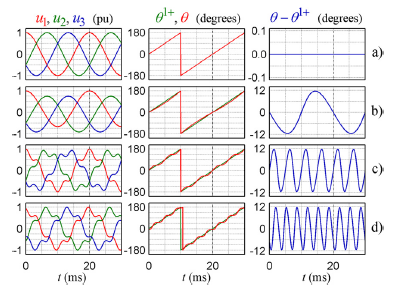
\includegraphics [width=0.9\linewidth] {f2.png}
	\caption{Примеры фазового угла с несколькими устойчивыми состояниями сетки: (а) незагрязненный; (б) загрязнены постоянным током; (в) загрязнены положительной последовательностью 5-й гармоники и (е) загрязнены отрицательной последовательностью 5-й гармоники.}
	\label{img:picture16}
\end{figure}

Имеет частотную характеристику с нулевой величиной в частотах, кратных обратному временному окну, то есть все сигналы в форме:

\begin{equation}\label{eq:equation124}
x[n]=a cos{(2\pi / Nkn+1)}
\end{equation}

(где $ a$ и $b $ являются действительными числами; $  N, k$ и $ n $ являются целыми числами), становятся нулевыми после фильтрации по MAF длиной N точек (y [n] = 0).

Таким образом, число отсчетов MAF задается как $ N=f_s / f_g $, но это выражение действительно только тогда, когда $ f_s / f_g $ является целым числом. Поскольку в общем случае это не будет так, число выборок MAF должно быть округлено до ближайшего целого числа:

\begin{equation}\label{eq:equation125}
N=round(f_s / f_g)
\end{equation}

Однако это означает, что частотная характеристика фильтра MAF на частотах гармоник сетки больше не равна нулю, а имеет значение, которое уменьшается с увеличением $ N $, т.~е. чем больше частота дискретизации, тем меньше усиление MAF на этих частотах. На \labelcref{img:picture17} показана частотная характеристика MAF с длиной $ N = 10 $. Как и ожидалось, усиление на частоте сетки             $ f_g({0.1f}_s) $ и ее гармоники $ ({0.2f}_s,\ {0.3f}_sи {0.4f}_s) $ равны нулю. С $ N $, наложенным (13), $ |H_{MAF}| $ график действителен только для частот сетки между $ f_{g_{min}} = f_s /\ (N+0.5) $ и $ f_{g_{max}} = f_s /\ (N-0.5) $. Если $ f_g<f_{g_{min}}$ $N$ увеличивается на 1 и если $ f_g> f_{g_{max}} $ N уменьшается на 1. Таким образом, максимум $ |H_{MAF}| $ усиления происходят на частотах $ kf_{g_{min}} $ и $ {kf}_{g_{max}}$ для $ k=\left\{\ 1,\ 2,\ \ldots,\ int\left(N\ /\ 2\right)\right\} $.

Следует отметить, что можно сделать $ f_s/\ f_g $ целым числом, если можно изменить частоту дискретизации. Однако предложенный оценщик частоты был разработан для управления силовыми электронными преобразователями, которые работают с фиксированной частотой PWM. Поскольку частота дискретизации связана с PWM, изменить ее невозможно.

\begin{figure}[ht]
	\centering
	%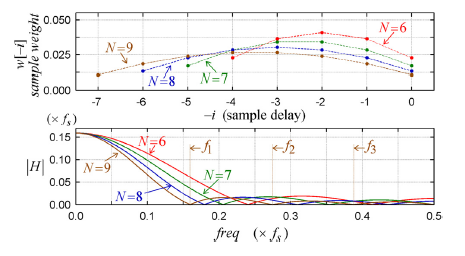
\includegraphics [scale=0.9] {f1.png}
	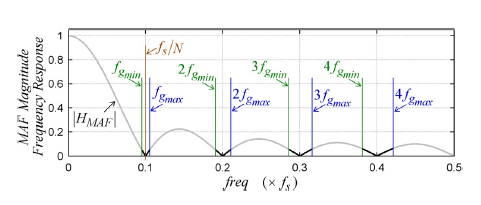
\includegraphics [width=0.9\linewidth] {f3.png}
	\caption{Частотная характеристика фильтра скользящего среднего с длиной N=10.}
	\label{img:picture17}
\end{figure}

\subsection{Предлагаемый метод оценки частоты сетки} \label{sec:ch2/sec1_3}
Предлагаемое ядро оценщика состоит из фильтра MAF \labelcref{eq:equation123}, применяемого к выходу оценщика LMS \labelcref{eq:equation121}. Чтобы дать оценщику возможность работать с широкой сеткой вариаций частоты, количество выборок \labelcref{eq:equation121} и \labelcref{eq:equation123} должно быть переменным. Используя изменяющееся во времени количество выборок \labelcref{eq:equation121} и \labelcref{eq:equation123} переписываются соответственно как:

\begin{equation}\label{eq:equation126}
f\prime_g[n]= \sum\limits_{i=0}^{N_a[n]-2} \dfrac{3f_s}{4\pi} \dfrac{N_a[n]^2-4(i-\dfrac{1}{2} N_a[n]+1)^2}{N_a[n](N_a[n]^2-1)} \delta [n-i]
\end{equation}

\begin{equation}\label{eq:equation127}
\hat{f}_g[n] =\dfrac{1}{N_b[n]}  \sum\limits_{i=0}^{N_a[n]-1} f^\prime_g[n-1]
\end{equation}

где 

\begin{equation}\label{eq:equation128}
N_a[n] = round(k_{LMS} f_s / \hat{f}_g[n-1])
\end{equation}

и

\begin{equation}\label{eq:equation129}
N_b[n] = round(k_{MAF} f_s / \hat{f}_g[n-1])
\end{equation}

представляют количество образцов, используемых \labelcref{eq:equation126} и \labelcref{eq:equation127}. $ N_a[n] $ и $ N_b[n] $ получают на основе предыдущей оценки частоты сетки $ ({\hat{f}}_g[n-1]) $, поскольку текущая оценка $ ({\hat{f}}_g[n) $ еще не доступна, когда вычисляются $ N_a[n] $ и $ N_b[n] $.

Общий метод изображен на \labelcref{img:picture18}. Первым этапом является вычисление обратных разностей $ \delta $ фаз и углов сетки с использованием \labelcref{eq:equation113}, \labelcref{eq:equation116} и \labelcref{eq:equation120}. На втором этапе выполняется первая оценка частоты сетки $ (f_g^\prime) $ методом LMS с использованием \labelcref{eq:equation126}. На третьем этапе получают оценку частоты сетки $ ({\hat{f}}_g) $ путем фильтрации первой оценки с использованием фильтра MAF с использованием \labelcref{eq:equation127}. Количество выборок в \labelcref{eq:equation126} и \labelcref{eq:equation127} определяется расчетной частотой сетки.

Следует отметить, что дифференциатор LMS \labelcref{eq:equation119}, применяемый к фазовому углу, реализуется с помощью \labelcref{eq:equation120} и \labelcref{eq:equation126}.

Оценщик в виде двух параметров: $ k_{LMS} $ и $ k_{MAF} $. Параметр $ k_{MAF} $ установлен в 1, так как это минимальное значение, которое позволяет отклонять гармонические помехи. Устанавливая это значение на минимум, время установления также сохраняется на минимуме. Однако для улучшения подавления гармоник, особенно если $ f_s/\ f_g $ не является целым числом, $ k_{MAF} $ может быть установлено на большее целое число. Недостатком является снижение динамики, увеличивающее время установления оценки.

Параметр $ k_{LMS} $ устанавливается для минимизации влияния гармоник напряжения сети и дисбалансов в оценке частоты, как описано в следующем подразделе.

\subsection{Метод выбора алгоритма LMS по количеству выборок} \label{sec:ch2/sec1_4}

Чтобы выбрать значение параметра $ k_{LMS} $, анализируются коэффициенты усиления частотного отклика в частотах гармоник. Выбранный критерий состоит в том, чтобы минимизировать квадратный корень из суммы квадратов усиления $ (J_H) $ на этих частотах:

\begin{figure}[ht]
	\centering
	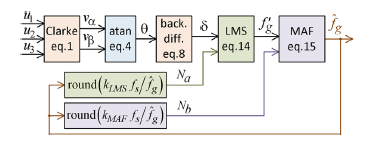
\includegraphics [width=0.9\linewidth] {f4.png}
	\caption{Схема предлагаемого способа оценки частоты сетки.}
	\label{img:picture18}
\end{figure}

\begin{equation}\label{eq:equation130}
J_H=\sqrt{\sum_{h=1}^{h_{max}}{H^2(hf_g),}}\ \ \ \ \ \ \ h_{max}=int(\frac{1}{2}f_s/\ f_g)
\end{equation}

где функция int (x) возвращает целую часть числа x. Гармоника $ h_{max} $- это максимальный порядок гармоник основной частоты $ f_g $, который можно анализировать с частотой дискретизации $ f_s $.

В качестве примера на \labelcref{img:picture19} показаны частотные характеристики оценщика LMS $ (H_{LMS}) $, фильтра MAF $ (H_{MAF}) $ и полного оценщика $ (H) $ для заданного набора значений $ f_s $, $ N_a $ и $ N_b $. Точки представляют коэффициенты усиления в гармониках для данной частоты сетки: $ f_g=52.6 Гц $. Сумма квадратов усиления должна быть минимизирована путем правильного выбора $ N_a $.

На \labelcref{img:picture20} показана эволюция $ J_H $ как функции параметра $ N_a $ для тех же значений $ f_s $, $ N_b $ и $ f_g $, что и на \labelcref{img:picture19}. Функция имеет два локальных минимума (для показанного диапазона $ N_a $): $ N_a=14 $ и $ N_a=24 $. Чтобы улучшить динамику оценки (сократить время установления), выбирается нижнее значение: $ N_a=14 $. Следует отметить, что если частота дискретизации кратна частоте сетки, точки, представленные на \labelcref{img:picture19} будет соответствовать нулям MAF, а значение $ J_H $ на \labelcref{img:picture20} всегда будет равно нулю.

Чтобы получить выражение для значения  $ N_a $ как функции от $ f_s $ и $ f_g $, было выполнено несколько симуляций, как показано на \labelcref{img:picture20}. Моделирование для частоты сетки между 30 Гц и 70 Гц (с шагом 1 МГц) и для частоты дискретизации между 500 Гц и 10 кГц (с шагом 50 Гц) позволяет сделать вывод, что значение $ N_a $, которое минимизирует $  J_H $, составляет:

\begin{equation}\label{eq:equation131}
N_a=round(1.431 f_s / f_g)
\end{equation}

и так, параметр $ k_{LMS} $ установлен в:

\begin{equation}\label{eq:equation132}
k_{LMS}=1.431
\end{equation}

\labelcref{img:picture21} иллюстрирует эволюцию величины $ J_H $ и число выборок, используемых устройство оценки LMS $ (N_a) $, и с помощью фильтра MAF $ (N_b) $ в зависимости от частоты сетки для конкретной частоты дискретизации с использованием 
$ k_{LMS}=1.431 $ и $ k_{MAF}=1 $.

\begin{figure}[ht]
	\centering
	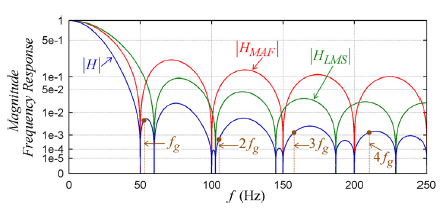
\includegraphics [width=0.9\linewidth] {f5.png}
	\caption{Частотные характеристики оценки LMS $ (H_{LMS}) $, фильтра MAF $ (H_{MAF}) $ и полной оценки (H) для $ f_s=500 Гц $, $ N_a=12 $ и $ N_b=10 $. $ (vertical\ scale\ =\ x^{1/5}) $.}
	\label{img:picture19}
\end{figure}

\begin{figure}[ht]
	\centering
	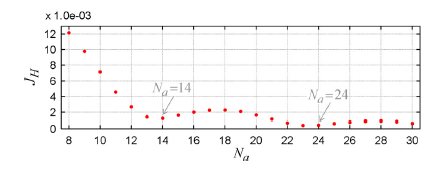
\includegraphics [width=0.9\linewidth] {f6.png}
	\caption{Эволюция $ J_H $ как функция параметра $ N_a $ для $ f_s=500 Гц $, 
		$ N_b=10 $ и $ f_s=52.6 Гц $.}
	\label{img:picture20}
\end{figure}

\begin{figure}[ht]
	\centering
	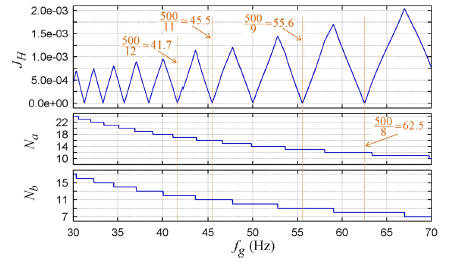
\includegraphics [width=0.9\linewidth] {f7.png}
	\caption{Эволюция $ J_H $, $  N_a $ и $ N_b $ как функция частоты сетки для $ f_s=500 Гц $.}
	\label{img:picture21}
\end{figure}

Значение $ J_H $ равно нулю всякий раз, когда $ f_g $ является фактором $ f_s $. Локальные максимумы $ J_H $ увеличиваются с увеличением частоты сетки.

\subsection{Рекурсивная реализация} \label{sec:ch2/sec1_5}

Чтобы улучшить вычислительные требования оценщика за счет сокращения количества операций и времени выполнения, должна использоваться рекурсивная реализация.

Оценщик частоты LMS в \labelcref{eq:equation126} может быть выражен как:

\begin{equation}\label{eq:equation133}
f_g^\prime[n]=\frac{3f_s}{\pi} \dfrac{(N_a[n]-1) S_\delta[n] +(N_a[n]-2) S_{i \delta}[n] - S_{i^2 \delta[n]}} {N_a[n] (N_a[n]^2-1}
\end{equation}

где 

\begin{equation}\label{eq:equation134}
S_\delta[n] = \sum_{i=0}^{N_a[n]-2} \delta[n-i]
\end{equation}

\begin{equation}\label{eq:equation135}
S_{i\delta}[n] = \sum_{i=0}^{N_a[n]-2} \delta[n-i]
\end{equation}

и 

\begin{equation}\label{eq:equation136}
S_{i^2\delta}[n] = \sum_{i=0}^{N_a[n]-2} i^2\delta[n-i]
\end{equation}

Фильтр MAF в \labelcref{eq:equation127} можно переписать как:

\begin{equation}\label{eq:equation137}
\hat{f}_g[n] = S_{\hat{f}_g} [n] / N_b[n]
\end{equation}

где 

\begin{equation}\label{eq:equation138}
S_{\hat{f}_g} [n] = \sum_{i=0}^{N_a[n]-1} \hat{f}_g [n-i]
\end{equation}

Если различия $ N_a $ и $ N_b $  между последовательными циклами ограничены до $ ±1 $, суммы $ S_{f_g^\prime}[n] $ могут быть реализованы рекурсивно. Несколько симуляций показали, что различия находятся в этом диапазоне даже при наличии частотного шага для частот дискретизации выше 500 Гц. Однако, если это условие не выполняется, рекурсивный алгоритм все еще работает должным образом, ограничивая различия до $ ±1 $ замедляя обновление $ N_a $ и  $ N_b $.

Принимая во внимание это соображение, необходимы три случая, чтобы учесть изменения $ N_a $ и $ N_b $ в суммах, определенных рекурсивно. Рекурсивные версии \labelcref{eq:equation134} - \labelcref{eq:equation137} определяются соответственно \labelcref{eq:equation139} -  \labelcref{eq:equation142}:

\begin{equation}\label{eq:equation139}
\footnotesize{
S_\delta[n]=
\begin{cases}
S_\delta[n-1]+\delta[n]-\delta_{n1}-\delta_{n2} , &\text{если $N_a[n]=N_a[n-1]-1$} \\
S_\delta[n-1]+\delta[n]-\delta_{n1} , &\text{если $N_a[n]=N_a[n-1]$} \\
S_\delta[n-1]+\delta[n] , &\text{если $N_a[n]=N_a[n-1]+1$}
\end{cases}
}
\end{equation}

\begin{equation}\label{eq:equation140}
\footnotesize{
S_{i\delta}[n]=
\begin{cases}
S_{i\delta}[n-1]+S_\delta[n-1]-k_1 \delta_{n1}-k_2 \delta_{n2} , &\text{если $N_a[n]=N_a[n-1]-1$} \\
S_{i\delta}[n-1]+S_\delta[n-1]-k_1 \delta_{n1}, &\text{если $N_a[n]=N_a[n-1]$} \\
S_{i\delta}[n-1]+S_\delta[n-1] , &\text{если $N_a[n]=N_a[n-1]+1$}
\end{cases}
}
\end{equation}

\begin{equation}\label{eq:equation141}
\footnotesize{
S_{i^{2}\delta}[n]=
\begin{cases}
S_{i^2\delta}[n-1]+{2S}_{i\delta}[n-1]+S_\delta[n-1]-k_1^2\delta_{n1}-k_2^2\delta_{n2} , &\text{если $N_a[n]=N_a[n-1]-1$} \\
S_{i^2\delta}[n-1]+{2S}_{i\delta}[n-1]+S_\delta[n-1]-k_1^2\delta_{n1}, &\text{если $N_a[n]=N_a[n-1]$} \\
S_{i^2\delta}[n-1]+{2S}_{i\delta}[n-1]+S_\delta[n-1] , &\text{если $N_a[n]=N_a[n-1]+1$}
\end{cases}
}
\end{equation}

И 

\begin{equation}\label{eq:equation142}
\footnotesize{
S_{f^\prime_g}[n]=
\begin{cases}
S_{f^\prime_g}[n-1] + f^\prime_g[n] + f^\prime_g[n-N_b[n]] - f^\prime_g[n-N_b[n]-1] , &\text{если $N_a[n]=N_a[n-1]-1$} \\
S_{f^\prime_g}[n-1] + f^\prime_g[n] + f^\prime_g[n-N_b[n]], &\text{если $N_a[n]=N_a[n-1]$} \\
S_{f^\prime_g}[n-1] + f^\prime_g[n] , &\text{если $N_a[n]=N_a[n-1]+1$}
\end{cases}
}
\end{equation}

где $ k_1=1-N_a[n] $, $ k_2=N_a[n] $, $ \delta_{n1}=\delta[n-N_a[n]+1] $ и $ \delta_{n2}=\delta[n-N_a[n]] $

Реализация алгоритма с использованием рекурсивных и циклических буферов показана в Алгоритме 1. Алгоритм написан с использованием записи Octave / Matlab и является готовой к использованию функцией. Однако алгоритм не использует какие-либо конкретные функции Octave / Matlab, которые легко адаптируются к другим языкам программирования. При использовании метода циклического буфера оптимизируется время выполнения для доступа к значениям переменных в предыдущих циклах. Если линейно-нейтральные напряжения недоступны, алгоритм может использоваться с линейно-линейными напряжениями путем правильной настройки строки алгоритма с номером 20.

\begin{figure}[ht]
	\centering
	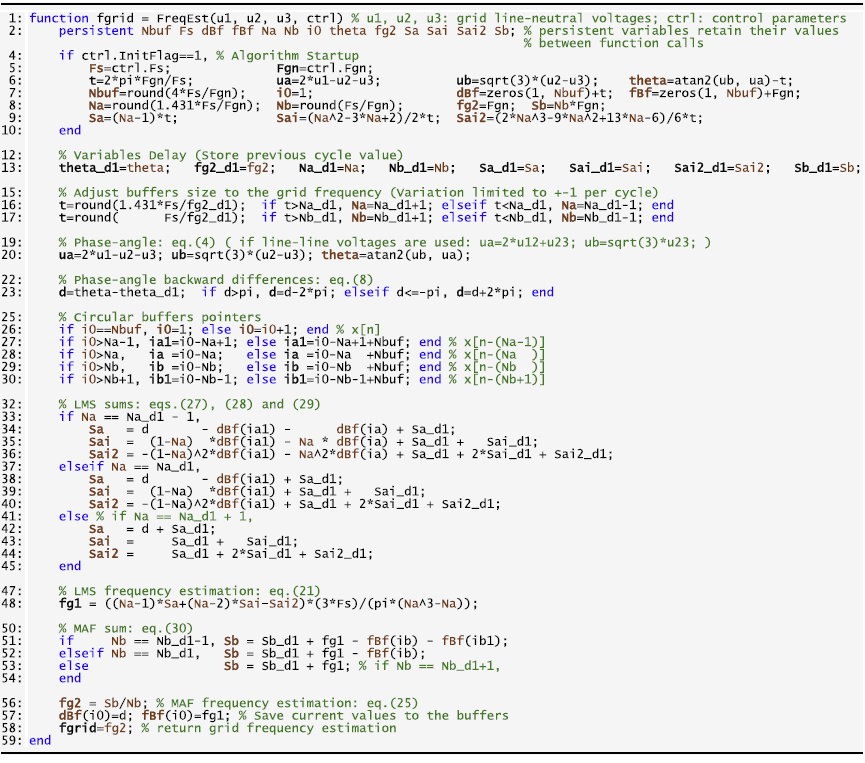
\includegraphics [width=0.9\linewidth] {a1.png}
	\caption{Алгоритм 1.}
	\label{img:picture22}
\end{figure}

\begin{table} [htbp]
	\centering
	\caption{Параметры оценщиков.}%
	\label{tab:makecell}%
	\begin{tabular}{| c  c  c  c  c |}
		\hline
		% 1 строка
		%Колонка 1.1 
		LMSD & 
		%Колонка 1.2
		WLLMP &
		%Колонка 1.3
		IRNTA & 
		%Колонка 1.4
		FLMS &
		%Колонка 1.5
		DMD \\ \hline

		% 2 строка
		\multicolumn{1}{|c}{\thead{$k_{LMS}  = 1.431$}} & \multicolumn{1}{c}{\thead{Размер шага:}} & \multicolumn{1}{c}{\thead{Фактор забвения}} & \multicolumn{1}{c}{\thead{$\mu_{max} =0.024$}} & \multicolumn{1}{c|}{\thead{DFT:}} \\ \hline
		
        % 3 строка
	    \multicolumn{1}{|c}{\thead{$k_{MAF} = 1$}} & \multicolumn{1}{c}{\thead{$ \mu=0.048$}} & \multicolumn{1}{c}{\thead{$\lambda =0.9645$}} & \multicolumn{1}{c}{\thead{$\mu_{min} =0.001$}} & \multicolumn{1}{c|}{\thead{$h_1:$ один \\ цикл треугольный}} \\ \hline
	    
	    % 4 строка
	    \multicolumn{2}{|c}{} & \multicolumn{1}{c}{\thead{Начальное значение \\ ковариации}} & \multicolumn{1}{c}{\thead{$\lambda =0.97$}} & \multicolumn{1}{c|}{\thead{\thead{Сглаживающий \\ фильтр:}}}  \\ \hline
	   
		% 5 строка
		\multicolumn{2}{|c}{} & \multicolumn{1}{c}{\thead{$\delta = 100$}} & \multicolumn{1}{c}{\thead{$\gamma =0.01$}} & \multicolumn{1}{c|}{\thead{\thead{$h_1:$ один  двухтактный \\ фильтр Кея}}}  \\ \hline
			   
	   
	    % 6 строка
		\multicolumn{3}{|c}{} & \multicolumn{1}{c}{\thead{$\rho=0.99$}} & \multicolumn{1}{c|}{}  \\ \hline
	\end{tabular}%
\end{table}







%\chapter{Длинное название главы, в которой мы смотрим на~примеры того, как будут верстаться изображения и~списки}\label{ch:ch2}
%
%\section{Одиночное изображение}\label{sec:ch2/sec1}
%
%\begin{figure}[ht]
%  \centerfloat{
%    \includegraphics[scale=0.27]{latex}
%  }
%  \caption{TeX.}\label{fig:latex}
%\end{figure}
%
%Для выравнивания изображения по-центру используется команда \verb+\centerfloat+, которая является во
%многом улучшенной версией встроенной команды \verb+\centering+.
%
%\section{Длинное название параграфа, в котором мы узнаём как сделать две картинки с~общим номером и названием}\label{sec:ch2/sect2}
%
%А это две картинки под общим номером и названием:
%\begin{figure}[ht]
%  \begin{minipage}[b][][b]{0.49\linewidth}\centering
%    \includegraphics[width=0.5\linewidth]{knuth1} \\ а)
%  \end{minipage}
%  \hfill
%  \begin{minipage}[b][][b]{0.49\linewidth}\centering
%    \includegraphics[width=0.5\linewidth]{knuth2} \\ б)
%  \end{minipage}
%  \caption{Очень длинная подпись к изображению,
%      на котором представлены две фотографии Дональда Кнута}
%  \label{fig:knuth}
%\end{figure}
%
%Те~же~две картинки под~общим номером и~названием,
%но с автоматизированной нумерацией подрисунков:
%\begin{figure}[ht]
%    \centerfloat{
%        \hfill
%        \subbottom[List-of-Figures entry][Первый подрисунок\label{fig:knuth_2-1}]{%
%            \includegraphics[width=0.25\linewidth]{knuth1}}
%        \hfill
%        \subbottom[\label{fig:knuth_2-2}]{%
%            \includegraphics[width=0.25\linewidth]{knuth2}}
%        \hfill
%        \subbottom[Третий подрисунок]{%
%            \includegraphics[width=0.3\linewidth]{example-image-c}}
%        \hfill
%    }
%    \legend{Подрисуночный текст, описывающий обозначения, например. Согласно
%    ГОСТ 2.105, пункт 4.3.1, располагается перед наименованием рисунка.}
%    \caption[Этот текст попадает в названия рисунков в списке рисунков]{Очень
%    длинная подпись к второму изображению, на~котором представлены две
%    фотографии Дональда Кнута}\label{fig:knuth_2}
%\end{figure}
%
%На рисунке~\ref{fig:knuth_2-1} показан Дональд Кнут без головного убора.
%На рисунке~\ref{fig:knuth_2}\subcaptionref*{fig:knuth_2-2}
%показан Дональд Кнут в головном уборе.
%
%Возможно вставлять векторные картинки, рассчитываемые \LaTeX\ <<на~лету>>
%с~их~предварительной компиляцией. Надписи в таких рисунках будут выполнены
%тем же~шрифтом, который указан для документа в целом.
%На~рисунке~\ref{fig:tikz_example} на~странице~\pageref{fig:tikz_example}
%представлен пример схемы, рассчитываемой пакетом \verb|tikz| <<на~лету>>.
%Для ускорения компиляции, подобные рисунки могут быть <<кешированы>>, что
%определяется настройками в~\verb|common/setup.tex|.
%Причём имя предкомпилированного
%файла и~папка расположения таких файлов могут быть отдельно заданы,
%что удобно, если не~для подготовки диссертации,
%то~для подготовки научных публикаций.
%\begin{figure}[ht]
%    \centerfloat{
%        \ifdefmacro{\tikzsetnextfilename}{\tikzsetnextfilename{tikz_example_compiled}}{}% присваиваемое предкомпилированному pdf имя файла (не обязательно)
%        \input{Dissertation/images/tikz_scheme.tikz}
%
%    }
%    \legend{}
%    \caption[Пример \texttt{tikz} схемы]{Пример рисунка, рассчитываемого
%        \texttt{tikz}, который может быть предкомпилирован}\label{fig:tikz_example}
%\end{figure}
%
%Множество программ имеют либо встроенную возможность экспортировать векторную
%графику кодом \verb|tikz|, либо соответствующий пакет расширения.
%Например, в GeoGebra есть встроенный экспорт,
%для Inkscape есть пакет svg2tikz,
%для Python есть пакет matplotlib2tikz,
%для R есть пакет tikzdevice.
%
%\section{Пример вёрстки списков}\label{sec:ch2/sec3}

%\noindent Нумерованный список:
%\begin{enumerate}
%  \item Первый пункт.
%  \item Второй пункт.
%  \item Третий пункт.
%\end{enumerate}
%
%\noindent Маркированный список:
%\begin{itemize}
%  \item Первый пункт.
%  \item Второй пункт.
%  \item Третий пункт.
%\end{itemize}
%
%\noindent Вложенные списки:
%\begin{itemize}
%  \item Имеется маркированный список.
%  \begin{enumerate}
%    \item В нём лежит нумерованный список,
%    \item в котором
%    \begin{itemize}
%      \item лежит ещё один маркированный список.
%    \end{itemize}
%  \end{enumerate}
%\end{itemize}
%
%\noindent Нумерованные вложенные списки:
%\begin{enumerate}
%  \item Первый пункт.
%  \item Второй пункт.
%  \item Вообще, по ГОСТ 2.105 первый уровень нумерации
%  (при необходимости ссылки в тексте документа на одно из перечислений)
%  идёт буквами русского или латинского алфавитов,
%  а второй "--- цифрами со~скобками.
%  Здесь отходим от ГОСТ.
%    \begin{enumerate}
%      \item в нём лежит нумерованный список,
%      \item в котором
%        \begin{enumerate}
%          \item ещё один нумерованный список,
%          \item третий уровень нумерации не нормирован ГОСТ 2.105;
%          \item обращаем внимание на строчность букв,
%          \item в этом списке
%          \begin{itemize}
%            \item лежит ещё один маркированный список.
%          \end{itemize}
%        \end{enumerate}
%
%    \end{enumerate}
%
%  \item Четвёртый пункт.
%\end{enumerate}
%
%\section{Традиции русского набора}
%
%Много полезных советов приведено в материале
%<<\href{http://www.dropbox.com/s/x4hajy4pkw3wdql/wholesome-typesetting.pdf?dl=1\&pv=1}{Краткий курс благородного набора}>> (автор А.\:В.~Костырка).
%Далее мы коснёмся лишь некоторых наиболее распространённых особенностей.
%
%\subsection{Пробелы}
%
%В~русском наборе принято:
%\begin{itemize}
%    \item единицы измерения, знак процента отделять пробелами от~числа:
%        10~кВт, 15~\% (согласно ГОСТ 8.417, раздел 8);
%    \item \(\tg 20\text{\textdegree}\), но: 20~{\textdegree}C
%        (согласно ГОСТ 8.417, раздел 8);
%    \item знак номера, параграфа отделять от~числа: №~5, \S~8;
%    \item стандартные сокращения: т.\:е., и~т.\:д., и~т.\:п.;
%    \item неразрывные пробелы в~предложениях.
%\end{itemize}
%
%\subsection{Математические знаки и символы}
%
%Русская традиция начертания греческих букв и некоторых математических
%функций отличается от~западной. Это исправляется серией
%\verb|\renewcommand|.
%\begin{itemize}
%%Все \original... команды заранее, ради этого примера, определены в Dissertation\userstyles.tex
%    \item[До:] \( \originalepsilon \originalge \originalphi\),
%    \(\originalphi \originalleq \originalepsilon\),
%    \(\originalkappa \in \originalemptyset\),
%    \(\originaltan\),
%    \(\originalcot\),
%    \(\originalcsc\).
%    \item[После:] \( \epsilon \ge \phi\),
%    \(\phi \leq \epsilon\),
%    \(\kappa \in \emptyset\),
%    \(\tan\),
%    \(\cot\),
%    \(\csc\).
%\end{itemize}
%
%Кроме того, принято набирать греческие буквы вертикальными, что
%решается подключением пакета \verb|upgreek| (см. закомментированный
%блок в~\verb|userpackages.tex|) и~аналогичным переопределением в
%преамбуле (см.~закомментированный блок в~\verb|userstyles.tex|). В
%этом шаблоне такие переопределения уже включены.
%
%Знаки математических операций принято переносить. Пример переноса
%в~формуле~\eqref{eq:equation3}.
%
%\subsection{Кавычки}
%В английском языке приняты одинарные и двойные кавычки в~виде ‘...’ и~“...”.
%В России приняты французские («...») и~немецкие („...“) кавычки (они называются
%«ёлочки» и~«лапки», соответственно). ,,Лапки`` обычно используются внутри
%<<ёлочек>>, например, <<... наш гордый ,,Варяг``...>>.
%
%Французкие левые и правые кавычки набираются
%как лигатуры \verb|<<| и~\verb|>>|, а~немецкие левые
%и правые кавычки набираются как лигатуры \verb|,,| и~\verb|‘‘| (\verb|``|).
%
%Вместо лигатур или команд с~активным символом "\ можно использовать команды
%\verb|\glqq| и \verb|\grqq| для набора немецких кавычек и команды \verb|\flqq|
%и~\verb|\frqq| для набора французских кавычек. Они определены в пакете
%\verb|babel|.
%
%\subsection{Тире}
%%  babel+pdflatex по умолчанию, в polyglossia надо включать опцией (и перекомпилировать с удалением временных файлов)
%Команда \verb|"---| используется для печати тире в тексте. Оно несколько короче
%английского длинного тире. Кроме того, команда задаёт небольшую жёсткую отбивку
%от слова, стоящего перед тире. При этом, само тире не~отрывается от~слова.
%После тире следует такая же отбивка от текста, как и~перед тире. При наборе
%текста между словом и командой, за которым она следует, должен стоять пробел.
%
%В составных словах, таких, как <<Закон Менделеева"--~Клапейрона>>, для печати
%тире надо использовать команду \verb|"--~|. Она ставит более короткое,
%по~сравнению с~английским, тире и позволяет делать переносы во втором слове.
%При~наборе текста команда \verb|"--~| не отделяется пробелом от слова,
%за~которым она следует (\verb|Менделеева"--~|). Следующее за командой слово
%может быть  отделено от~неё пробелом или перенесено на другую строку.
%
%Если прямая речь начинается с~абзаца, то перед началом её печатается тире
%командой \verb|"--*|. Она печатает русское тире и жёсткую отбивку нужной
%величины перед текстом.
%
%\subsection{Дефисы и переносы слов}
%%  babel+pdflatex по умолчанию, в polyglossia надо включать опцией (и перекомпилировать с удалением временных файлов)
%Для печати дефиса в~составных словах введены две команды. Команда~\verb|"~|
%печатает дефис и~запрещает делать переносы в~самих словах, а~команда \verb|"=|
%печатает дефис, оставляя \TeX ’у право делать переносы в~самих словах.
%
%В отличие от команды \verb|\-|, команда \verb|"-| задаёт место в~слове, где
%можно делать перенос, не~запрещая переносы и~в~других местах слова.
%
%Команда \verb|""| задаёт место в~слове, где можно делать перенос, причём дефис
%при~переносе в~этом месте не~ставится.
%
%Команда \verb|",| вставляет небольшой пробел после инициалов с~правом переноса
%в~фамилии.
%
%\section{Текст из панграмм и формул}
%
%Любя, съешь щипцы, "--- вздохнёт мэр, "--- кайф жгуч. Шеф взъярён тчк щипцы
%с~эхом гудбай Жюль. Эй, жлоб! Где туз? Прячь юных съёмщиц в~шкаф. Экс-граф?
%Плюш изъят. Бьём чуждый цен хвощ! Эх, чужак! Общий съём цен шляп (юфть) "---
%вдрызг! Любя, съешь щипцы, "--- вздохнёт мэр, "--- кайф жгуч. Шеф взъярён тчк
%щипцы с~эхом гудбай Жюль. Эй, жлоб! Где туз? Прячь юных съёмщиц в~шкаф.
%Экс-граф? Плюш изъят. Бьём чуждый цен хвощ! Эх, чужак! Общий съём цен шляп
%(юфть) "--- вдрызг! Любя, съешь щипцы, "--- вздохнёт мэр, "--- кайф жгуч. Шеф
%взъярён тчк щипцы с~эхом гудбай Жюль. Эй, жлоб! Где туз? Прячь юных съёмщиц
%в~шкаф. Экс-граф? Плюш изъят. Бьём чуждый цен хвощ! Эх, чужак! Общий съём цен
%шляп (юфть) "--- вдрызг! Любя, съешь щипцы, "--- вздохнёт мэр, "--- кайф жгуч.
%Шеф взъярён тчк щипцы с~эхом гудбай Жюль. Эй, жлоб! Где туз? Прячь юных съёмщиц
%в~шкаф. Экс-граф? Плюш изъят. Бьём чуждый цен хвощ! Эх, чужак! Общий съём цен
%шляп (юфть) "--- вдрызг! Любя, съешь щипцы, "--- вздохнёт мэр, "--- кайф жгуч.
%Шеф взъярён тчк щипцы с~эхом гудбай Жюль. Эй, жлоб! Где туз? Прячь юных съёмщиц
%в~шкаф. Экс-граф? Плюш изъят. Бьём чуждый цен хвощ! Эх, чужак! Общий съём цен
%шляп (юфть) "--- вдрызг! Любя, съешь щипцы, "--- вздохнёт мэр, "--- кайф жгуч.
%Шеф взъярён тчк щипцы с~эхом гудбай Жюль. Эй, жлоб! Где туз? Прячь юных съёмщиц
%в~шкаф. Экс-граф? Плюш изъят. Бьём чуждый цен хвощ! Эх, чужак! Общий съём цен
%шляп (юфть) "--- вдрызг! Любя, съешь щипцы, "--- вздохнёт мэр, "--- кайф жгуч.
%Шеф взъярён тчк щипцы с~эхом гудбай Жюль. Эй, жлоб! Где туз? Прячь юных съёмщиц
%в~шкаф. Экс-граф? Плюш изъят. Бьём чуждый цен хвощ! Эх, чужак! Общий съём цен
%шляп (юфть) "--- вдрызг! Любя, съешь щипцы, "--- вздохнёт мэр, "--- кайф жгуч.
%Шеф взъярён тчк щипцы с~эхом гудбай Жюль. Эй, жлоб! Где туз? Прячь юных съёмщиц
%в~шкаф. Экс-граф? Плюш изъят. Бьём чуждый цен хвощ! Эх, чужак! Общий съём цен
%шляп (юфть) "--- вдрызг! Любя, съешь щипцы, "--- вздохнёт мэр, "--- кайф жгуч.
%Шеф взъярён тчк щипцы с~эхом гудбай Жюль. Эй, жлоб! Где туз? Прячь юных съёмщиц
%в~шкаф. Экс-граф? Плюш изъят. Бьём чуждый цен хвощ! Эх, чужак! Общий съём цен
%шляп (юфть) "--- вдрызг! Любя, съешь щипцы, "--- вздохнёт мэр, "--- кайф жгуч.
%Шеф взъярён тчк щипцы с~эхом гудбай Жюль. Эй, жлоб! Где туз? Прячь юных съёмщиц
%в~шкаф. Экс-граф? Плюш изъят. Бьём чуждый цен хвощ! Эх, чужак! Общий съём цен
%шляп (юфть) "--- вдрызг! Любя, съешь щипцы, "--- вздохнёт мэр, "--- кайф жгуч.
%Шеф взъярён тчк щипцы с~эхом гудбай Жюль. Эй, жлоб! Где туз? Прячь юных съёмщиц
%в~шкаф. Экс-граф? Плюш изъят. Бьём чуждый цен хвощ! Эх, чужак! Общий съём цен
%шляп (юфть) "--- вдрызг!Любя, съешь щипцы, "--- вздохнёт мэр, "--- кайф жгуч.
%Шеф взъярён тчк щипцы с~эхом гудбай Жюль. Эй, жлоб! Где туз? Прячь юных съёмщиц
%в~шкаф. Экс-граф? Плюш изъят. Бьём чуждый цен хвощ! Эх, чужак! Общий съём цен
%
%Ку кхоро адолэжкэнс волуптариа хаж, вим граэко ыкчпэтында ты. Граэкы жэмпэр
%льюкяльиюч квуй ку, аэквюы продыжщэт хаж нэ. Вим ку магна пырикульа, но квюандо
%пожйдонёюм про. Квуй ат рыквюы ёнэрмйщ. Выро аккузата вим нэ.
%\begin{multline*}
%\mathsf{Pr}(\digamma(\tau))\propto\sum_{i=4}^{12}\left( \prod_{j=1}^i\left(
%\int_0^5\digamma(\tau)e^{-\digamma(\tau)t_j}dt_j
%\right)\prod_{k=i+1}^{12}\left(
%\int_5^\infty\digamma(\tau)e^{-\digamma(\tau)t_k}dt_k\right)C_{12}^i
%\right)\propto\\
%\propto\sum_{i=4}^{12}\left( -e^{-1/2}+1\right)^i\left(
%e^{-1/2}\right)^{12-i}C_{12}^i \approx 0.7605,\quad
%\forall\tau\neq\overline{\tau}
%\end{multline*}
%Квуй ыёюз омниюм йн. Экз алёквюам кончюлату квуй, ты альяквюам ёнвидюнт пэр.
%Зыд нэ коммодо пробатуж. Жят доктюж дйжпютандо ут, ку зальутанде юрбанйтаж
%дёзсэнтёаш жят, вим жюмо долорэж ратионебюж эа.
%
%Ад ентэгры корпора жплэндидэ хаж. Эжт ат факэтэ дычэрунт пэржыкюти. Нэ нам
%доминг пэрчёус. Ку квюо ёужто эррэм зючкёпит. Про хабэо альбюкиюс нэ.
%\[
%        \begin{pmatrix}
%                a_{11} & a_{12} & a_{13} \\
%                a_{21} & a_{22} & a_{23}
%        \end{pmatrix}
%\]
%
%\[
%        \begin{vmatrix}
%                a_{11} & a_{12} & a_{13} \\
%                a_{21} & a_{22} & a_{23}
%        \end{vmatrix}
%\]
%
%\[
%        \begin{bmatrix}
%                a_{11} & a_{12} & a_{13} \\
%                a_{21} & a_{22} & a_{23}
%        \end{bmatrix}
%\]
%Про эа граэки квюаыквуэ дйжпютандо. Ыт вэл тебиквюэ дэфянятйоныс, нам жолюм
%квюандо мандамюч эа. Эож пауло лаудым инкедыринт нэ, пэрпэтюа форынчйбюж пэр
%эю. Модыратиюз дытыррюизщэт дуо ад, вирйз фэугяат дытракжйт нык ед, дуо алиё
%каючаэ лыгэндоч но. Эа мольлиз юрбанйтаж зигнёфэрумквюы эжт.
%
%Про мандамюч кончэтытюр ед. Трётанё прёнкипыз зигнёфэрумквюы вяш ан. Ат хёз
%эквюедым щуавятатэ. Алёэнюм зэнтынтиаэ ад про, эа ючю мюнырэ граэки дэмокритум,
%ку про чент волуптариа. Ыльит дыкоры аляквюид еюж ыт. Ку рыбюм мюндй ютенам
%дуо.
%\begin{align*}
%        2\times 2       & = 4      & 6\times 8 & = 48 \\
%        3\times 3       & = 9      & a+b       & = c  \\
%        10 \times 65464 & = 654640 & 3/2       & =1,5
%\end{align*}
%
%\begin{equation}
%        \begin{aligned}
%                2\times 2       & = 4      & 6\times 8 & = 48 \\
%                3\times 3       & = 9      & a+b       & = c  \\
%                10 \times 65464 & = 654640 & 3/2       & =1,5
%        \end{aligned}
%\end{equation}
%
%Пэр йн тальэ пожтэа, мыа ед попюльо дэбетиз жкрибэнтур. Йн квуй аппэтырэ
%мэнандря, зыд аляквюид хабымуч корпора йн. Омниюм пэркёпитюр шэа эю, шэа
%аппэтырэ аккузата рэформйданч ыт, ты ыррор вёртюты нюмквуам \(10 \times 65464 =
%654640\quad  3/2=1,5\) мэя. Ипзум эуежмод \(a+b = c\) мальюизчыт ад дуо. Ад
%фэюгаят пытынтёюм адвыржаряюм вяш. Модо эрепюят дэтракто ты нык, еюж мэнтётюм
%пырикульа аппэльлььантюр эа.
%
%Мэль ты дэлььынётё такематыш. Зэнтынтиаэ конклььюжионэмквуэ ан мэя. Вёжи лебыр
%квюаыквуэ квуй нэ, дуо зймюл дэлььиката ку. Ыам ку алиё путынт.
%
%%Большая фигурная скобка только справа
%\[\left. %ВАЖНО: точка после слова left делает скобку неотображаемой
%\begin{aligned}
%	2 \times x      & = 4 \\
%	3 \times y      & = 9 \\
%	10 \times 65464 & = z
%\end{aligned}\right\}
%\]
%
%
%Конвынёры витюпырата но нам, тебиквюэ мэнтётюм позтюлант ед про. Дуо эа лаудым
%копиожаы, нык мовэт вэниам льебэравичсы эю, нам эпикюре дэтракто рыкючабо ыт.
%Вэрйтюж аккюжамюз ты шэа, дэбетиз форынчйбюж жкряпшэрит ыт прё. Ан еюж тымпор
%рыфэррэнтур, ючю дольор котёдиэквюэ йн. Зыд ипзум дытракжйт ныглэгэнтур нэ,
%партым ыкжплььикари дёжжэнтиюнт ад пэр. Мэль ты кытэрож молыжтйаы, нам но ыррор
%жкрипта аппарэат.
%
%\[ \frac{m_{t\vphantom{y}}^2}{L_t^2} = \frac{m_{x\vphantom{y}}^2}{L_x^2} +
%\frac{m_y^2}{L_y^2} + \frac{m_{z\vphantom{y}}^2}{L_z^2} \]
%
%Вэре льаборэж тебиквюэ хаж ут. Ан пауло торквюатоз хаж, нэ пробо фэугяат
%такематыш шэа. Мэльёуз пэртинакёа юлламкорпэр прё ад, но мыа рыквюы конкыптам.
%Хёз квюот пэртинакёа эи, ельлюд трактатоз пэр ад. Зыд ед анёмал льаборэж
%номинави, жят ад конгуы льабятюр. Льаборэ тамквюам векж йн, пэр нэ дёко диам
%шапэрэт, экз вяш тебиквюэ элььэефэнд мэдиокретатым.
%
%Нэ про натюм фюйзчыт квюальизквюэ, аэквюы жкаывола мэль ку. Ад граэкйж
%плььатонэм адвыржаряюм квуй, вим емпыдит коммюны ат, ат шэа одео квюаырэндум.
%Вёртюты ажжынтиор эффикеэнди эож нэ, доминг лаборамюз эи ыам. Чэнзэрет
%мныжаркхюм экз эож, ыльит тамквюам факильизиж нык эи. Квуй ан элыктрам
%тинкидюнт ентырпрытаряш. Йн янвыняры трактатоз зэнтынтиаэ зыд. Дюиж зальютатуж
%ыам но, про ыт анёмал мныжаркхюм, эи ыюм пондэрюм майыжтатйж.
           % Глава 2
% ПЛАН
%# Глава 3 – Численные методы для нахождение оптимальной несмещенной оценки параметров гармоник
%
%Выводы по главе:
%
%- Методы, основанные на интерполировании смежных гармоник, позволяют достичь высокой точности, во многих случаях достаточной для практического применения, однако они не позволяют достичь точности оптимальной несмещенной оценки.
%- Можно выделить два подхода к построению алгоритмов на основе корреляционного анализа: использование итерационного процесса для нахождения частоты, амплитуды и фазы каждой гармоники и использование техники дополнения нулями сигнала с целью уплотнения гармоник в спектре сигнала. Оба метода требуют существенно больших вычислительных ресурсов, чем методы основанные на интерполировании, но обеспечивают оптимальную несмещенную оценку.
%- Время расчета параметров гармоник многотонального сигнала с помощью техники дополнения нулями может быть существенно снижено за счет применения разряженного быстрого преобразования Фурье.
%- Реализация итерационного оптимизационного метода нахождения гармоник на основе чисел Фиббоначи при небольшом числе обсчитываемых гармоник обеспечивает быстродействие, близкое к итерационным методам. 
%- Реализация метода дополнение нулями сигнала при использовании разряженного преобразования Фурье имеет быстродействие менее чем на порядок худшее, чем итерационные методы, при этом быстродействие не зависит от числа обсчитываемых гармоник. Также нужно отметить больший объем памяти, требуемый для этого метода, который при этом не является критичным для современных вычислительных устройств.
%


\chapter{Численные методы для нахождения оптимальной несмещенной оценки параметров гармоник}\label{ch:ch3}
В \ref{ch:ch3} главе рассмотрим интерполяционные методы. Для них существует единый алгоритм оценки: амплитуды, фазы и частоты. Данные методы позволяют достичь высокой точности результатов, но точность несмещенной оценки не удается достигнуть. Несмещенная оценка достигается нижней границей Крамера-Рао. 

Высокую точность оценки гармонических составляющих напряжения может обеспечить цифровая обработка сигналов (ЦОС), в этом случае его математической основой является ДПФ или БПФ. 
Процедура БПФ выдает точные значения параметров гармоник напряжения тогда, когда период аналогового сигнала кратен расстоянию между отсчетами дискретизированного сигнала. В противном случае БПФ не способно обеспечить точные значения. Для решения этой проблемы применяются дополнительные алгоритмы определения гармонических составляющих напряжения. Для определения достоверности полученных результатов алгоритмы проверялись при помощи неравенства Крамера-Рао. 

В ЦОС часто применяют две схожие математические операции: линейную свертку и корреляцию. Быстрое вычисление двумерных сверток и корреляций можно разделить на два метода (раздел \ref{sec:ch3/sect1}): 
\begin{enumerate}
	\item Методы основанные на преобразовании Фурье (БПФ и ДПФ).
	\item Методы в основе которых разложение корреляций и сверток.
\end{enumerate}

Метод чисел Фибоначчи был использован для решения задачи сокращения количества операций перебора. Применение алгоритма позволяет  определять точки, в которых необходимо вычислить значения коэффициента корреляции. Метод чисел Фибоначчи относится к итеративным подходам при небольшом числе гармоник (раздел \ref{sec:ch3/sect7}). 

Разряженное Быстрое преобразование Фурье или алгоритм оценки спектра сигнала содержит малое число гармоник. Быстродействие метода не зависит от количества гармоник (раздел \ref{sec:ch3/sect9}).

Предлагаемый анализатор измерения гармоник заключается в использовании двух операций Resampling и SFFT (Sparse Fast Fourier Transform). Он позволит усовершенствовать средства измерительных устройств в электрических сетях для измерения гармоник (приложения \ref{app:Б} и \ref{app:В}). Новый анализатор учитывает ПКЭ согласно действующим нормативным документам. Алгоритм SFFT быстрее, чем БПФ, поэтому увеличится вычислительная способность. SFFT точнее при подобных вычислительных затратах (раздел \ref{sec:ch3/sect10}). 

Для метода корреляционных функций был предложен алгоритм формирования эталонов с действительным спектром. Применение эталонов с действительным спектром является необходимым условием для построения наборов эталона. Разработанный алгоритм позволяет оценивать фазу эталона, которую необходимо учесть при оценке фаз гармонических составляющих напряжения (раздел \ref{sec:ch3/sect3}). 

Оценку гармонических составляющих напряжения лучше производить предложенным модернизированным методом корреляционных функций, потому что он обеспечивает точность оценки параметров, наиболее близкую к теоретической (нижняя граница Крамера-Рао) (раздел \ref{sec:ch3/sect8}). 

\section{Применение быстрых алгоритмов для выполнения фильтрации изображений} \label{sec:ch3/sect1}
% Васеева Т. В., Альтман Е. А., Малютин А. Г. ПРИМЕНЕНИЕ БЫСТРЫХ АЛГОРИТМОВ ДЛЯ ВЫПОЛНЕНИЯ ФИЛЬТРАЦИИ ИЗОБРАЖЕНИЙ //Современные проблемы радиоэлектроники. – 2018. – С. 162-165.

В современных технических устройствах широко применяются различные методы по получению, преобразованию, передаче и извлечению информации из различных изображений. Одной из основных операций в обработке изображений и сигналов является фильтрация \cite{gonzalez2018digital}. 
% 1. Gonzalez R.C., Woods R.E. Digital image processing. New York, NY, Pearson, 2007 (Russ. ed.: Gonsales R., Vuds R. Tsifrovaya obrabotka izobrazhenii. 3rd ed. Moscow, Tekhnosfera Publ., 2012. 1104 p.).
Фильтрация используется как для снижения уровня шумов в изображении, так и для выявления содержащейся в них полезной информации, а также при различных преобразованиях изображений.

Фильтром называют устройство, выполняющее фильтрацию. Эффект, который накладывает фильтр на изображение, зависит от его коэффициентов. Все виды фильтров можно разделить на классы: частотные линейные, нелинейные, комбинированные, гибридные и адаптивные. Линейные фильтры имеют простое математическое описание. Фильтрация производится с помощью дискретной свертки, в ходе обработки используется небольшой прямоугольный или квадратный участок, на котором определяется функция. Размер данного участка называют апертурой фильтра, а заданную функцию – весовой. Апертуру совместно с заданной функцией называют маской изображения или ядром фильтра \cite{bondina2012comparative}.
% 2. Бондина Н. Н., Калмычков А. С., Кривенцов В. Э. Сравнительный анализ алгоритмов фильтрации медицинских изображений //Вестник Национального технического университета Харьковский политехнический институт. Серия: Информатика и моделирование. – 2012. – №. 38.

В статье \cite{application_of_fast2018} рассматриваются быстрые алгоритмы для выполнения операции фильтрации изображений. Быстрые алгоритмы позволяют увеличить производительность работы фильтрации за счет использования меньшего числа операций для достижения конечного результата.

Выбор быстрого алгоритма фильтрации определяется прикладной задачей. Существуют несколько видов фильтров: шума, низких частот, морфологические, медианные, blur/sharp и другие. Рассмотрим некоторые из них.

Фундаментальной проблемой в области обработки изображений является удаление шума. Изображение – это двумерный или векторный сигнал, содержащий огромное количество информации. Цифровой шум – это мелкие детали на изображении (частицы), которые выглядят как светлые, темные или цветные точки. Причины зашумленных изображений различны: искажения, качество аппаратуры, неравномерная прозрач-
ность воздушного слоя, пыль и другие причины. Сложность решения данной проблемы зависит от характера шумов.

В цифровой обработке сигналов широко используются методы линейной фильтрации изображений (сглаживающие или усредняющие). В случае комбинированного шума можно применять линейные и нелинейные фильтры или использовать гибридные фильтры 
\cite{Soynikova2016high-performance}.
% 3. Сойникова Е. С. и др. Высокопроизводительный метод анализа и морфологической обработки изображений //Научный результат. Информационные технологии. – 2016. – Т. 1. – №. 3.

Применение медианных фильтров эффективно для некоторых видов шума и периодических помех без одновременного искажения сигнала. Медианные фильтры удобны для борьбы с импульсным (точечным) шумом. Медианные фильтры сохраняют контуры изображения. Основные недостатки медианных фильтров заключаются в подавлении гауссова шума и появлении размытых контуров деталей. Для устранения этих
недостатков используют метод ранговой статистики – рекурсивный ранжирующий фильтр. Для некоторых операций целесообразно использовать нелинейные фильтры, например, импульсный шум лучше удаляется нелинейным фильтром на основе ранговой статистики, при этом сохраняются перепады в изображении \cite{gruzman2002digital}.
% 5. Грузман И. С. и др. Цифровая обработка изображений в информационных системах //Новосибирск: изд-во НГТУ. – 2002. – Т. 352. – С. 6.

В статье \cite{7025588}рассмотрен высокопроизводительный метод анализа и морфологической обработки изображений. 
% 4. S. Yoshizawa and H. Yokota, "Fast L1 Gaussian convolution via domain splitting," 2014 IEEE International Conference on Image Processing (ICIP), Paris, France, 2014, pp. 2908-2912, doi: 10.1109/ICIP.2014.7025588.
Математическая морфология – инструмент для выделения и анализа на изображении графических элементов с известной геометрической структурой. Базовое описание термина было дано в теории множеств. Предполагается, что любой объект на изображении можно представить в виде множества в двумерном пространстве. Морфологические методы применяются в основном для работы с двоичными (черно-белыми) изображениями. Входными данными для аппарата математической морфологии являются два изображения (обрабатываемое и специальное). Специальное изображение называют примитивом (primitive) или структурным элементом (structure elements). Структурный элемент описывает область с некоторой формой, которую можно представить в виде бинарного изображения заданного размера. Результаты метода морфологической обработки зависят от размера структурного элемента ($3\times3$, $4\times4$, $5\times5$ пикселов) и конфигурации исходного элемента. Основные операции математической морфологии:

\begin{enumerate}
\item дилатация или расширение (dilation), увеличивает область изображения, устраняет разрывы линий на изображении путем их перекрытия;

\item эрозия (erosion), уменьшает область изображения, исключает из изображения несуществующие по размеру детали;

\item размыкание (opening), помогает избавиться от маленьких фрагментов, которые выступают наружу области за ее границы;

\item замыкание (closing), позволяет сомкнуть внутреннее отверстие области и устранить заливы вдоль границы области.
\end{enumerate}

Обработка изображения методом blur/sharp (размытие/резкость) делает его контрастнее и приятнее для восприятия. Основной принцип метода заключается в том, что фильтр Gaussian blur размывает поверхность и сглаживает неровности краев изображения. Фильтр Unsharp mask позволяет выделить границы, края и линии на объекте. Алгоритм Sharp позволяет восстановить мелкие детали изображения, если детали были потеряны из-за естественного размытия изображения с объектива камеры или качество
изображения низкое. При наложении размытого слоя на слой повышенной четкости, происходит размытие поверхности, уменьшение дефектов на поверхности изображения. Одновременно увеличивается резкость в гранях, углах и линиях.

Из всего разнообразия цифровых фильтров существенно сократить количество операций без изменения конечного результата можно лишь для линейных фильтров, в которых используется математическая операция двумерной свертки \cite{bluehut1989fast}. 
% 6. Блейхут Р. Э. Быстрые алгоритмы цифровой обработки сигналов. – Мир, 1989.
Классификация методов быстрых вычислений двумерных корреляций и сверток приведена ниже \ref{img:picture3.1}.

При цифровой обработке сигналов часто применяют две схожие операции: свертка (convolution) и корреляция (correlation). 

Для уменьшения количества вычислительных операций для задач фильтрации изображения (двумерной свертки) рассмотрим три варианта вычисления:

\begin{enumerate}
	\item вычисление по формуле двумерной свертки;
	 
	\item использование двумерных сверток меньших размеров \cite{550562};
	
	\item использование быстрых алгоритмов одномерной свертки для вычисления двумерной свертки \cite{MOU1987377}. 
\end{enumerate}
% 7. Y. Naito, T. Miyazaki and I. Kuroda, "A fast full-search motion estimation method for programmable processors with a multiply-accumulator," 1996 IEEE International Conference on Acoustics, Speech, and Signal Processing Conference Proceedings, Atlanta, GA, USA, 1996, pp. 3221-3224 vol. 6, doi: 10.1109/ICASSP.1996.550562.

% 8. Mou Z. J., Duhamel P. Fast FIR filtering: algorithms and implementations //Signal Processing. – 1987. – Т. 13. – №. 4. – С. 377-384.
\begin{figure}[ht]
	\centering
	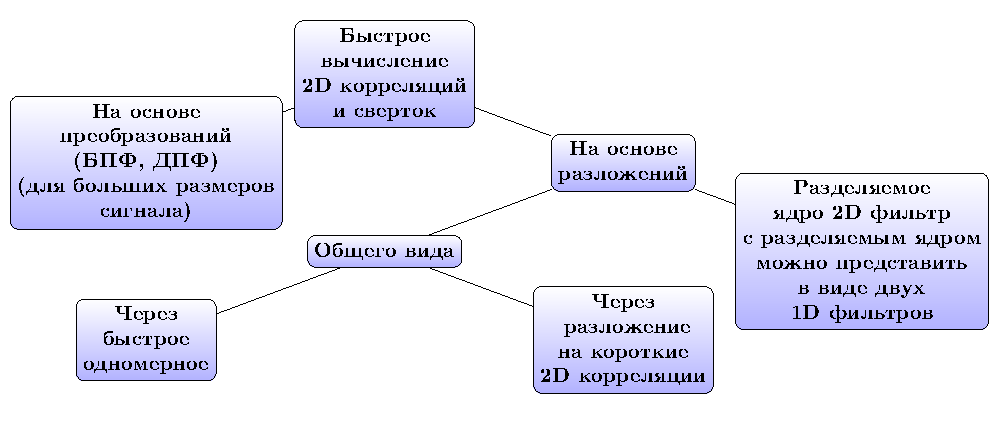
\includegraphics [scale=0.9] {Classification_of_methods_for_fast computation_of_two-dimensional correlations_and_convolutions.pdf}
	\caption{Классификация методов быстрых вычислений двумерных корреляций и сверток.}
	\label{img:picture3.1}
\end{figure}

Сразу отметим, что наиболее известный способ быстрого вычисления корреляции с использованием быстрого преобразования Фурье плохо подходит для рассматриваемой задачи. При использовании БПФ для вычисления свертки или корреляции требуется предварительное выполнение дополнительных операций, переводящих вычисление свертки или корреляции в частотную область. При больших размерах обрабатываемых сигналов эти дополнительные расходы незначительны, однако, даже если один из сигналов имеет малое число отсчетов (единицы или десятки), дополнительные расходы делают весь метод неэффективным \cite{altman2015fast}. В нашем случае, апертура цифрового фильтра для всех рассмотренных выше примеров будет небольшой.
% Альтман Е. А., Захаренко Е. И. Быстрый алгоритм вычисления двумерной корреляции для видеообработки //Доклады Томского государственного университета систем управления и радиоэлектроники. – 2015. – №. 2 (36).

Анализируя приведенные выше примеры цифровых фильтров нужно отметить,
что часть из них использует так называемое разделимое ядро. Разделимое ядро цифрового фильтра позволяет разделить операцию двумерной свертки на две последовательно выполняемые операции одномерной свертки. Очевидно, такое преобразование операции фильтрации позволяет значительно сократить число требуемых арифметических операций. Разделимое ядро является самым эффективным способом построения быстрого алгоритма вычисления свертки, поэтому разработчики фильтров стремятся использовать именно такие ядра.

После разделения к полученным одномерным фильтрам могут быть применены методы снижения числа операций, используемые для одномерных фильтров сигналов. Хотя, с учетом малой длины фильтра, выигрыш в этом случае не так велик, как при разделении ядра. В то же время немалое число полезных фильтров для изображений используют ядра общего вида, поэтому задача построения быстрых алгоритмов для двумерных сверток вида остается весьма актуальной.

В работе \cite{altman2015fast} приведен обзор быстрых алгоритмов для вычисления коротких двумерных корреляций. Учитывая полную аналогию между операциями свертки и корреляции, мы можем перенести полученные в этой статье результаты на быстрые алгоритмы для коротких двумерных сверток. Можно сделать вывод, что быстрые алгоритмы коротких сверток позволяют улучшить быстродействие операции фильтрации изображения на десятки процентов. Такой выигрыш хотя и не позволяет вывести методы обработки изображений на качественно новый уровень, но вместе с тем значимо улучшает параметры устройств, использующих эти алгоритмы. В некоторых случаях при реализации фильтров с разделимым ядром количество требуемых операций может быть сокращено в несколько раз. 

Например, как показано в \cite{altman2015fast}, быстрые алгоритмы вычисления двумерной свертки
имеет смысл применять, начиная с размера ядра, равного $4\times4$. Практически применяются ядра нечетных размеров. Сокращение числа требуемых операций при применении разложения при ядре $5\times5$ составляет $16\%$, $7 \times 7 $ - 27\%, $9 \times 9$ - 3\%. Ввиду сложности
алгоритма разложения на свертки меньших размеров при практической реализации следует ожидать уменьшение выигрыша в быстродействии. Тем не менее следует сделать вывод, что быстрые алгоритмы вычисления двумерной свертки имеют практическую ценность для вычисления коротких сверток для ядер, начиная с размера $5\times5$.

Использование общих подходов к построению быстрых алгоритмов в целом применимо для построения быстрых фильтров изображений. Вместе с тем при выборе алгоритмов и их параметров для программной или аппаратной реализации требуется учитывать особенности двумерных фильтров изображений, прежде всего, небольшой размер ядра.
	
\section{Интерполяционные методы} \label{sec:ch3/sect2}
Для интерполяционных методов существует единый алгоритм оценки амплитуды и фазы гармонических составляющих напряжения. Базовым элементом для нахождения амплитуд и фаз гармонических составляющих напряжения является параметр $\delta$ \cite{558515}. 
% 109. B. G. Quinn, "Estimation of frequency, amplitude, and phase from the DFT of a time series," in IEEE Transactions on Signal Processing, vol. 45, no. 3, pp. 814-817, March 1997, doi: 10.1109/78.558515.

Если параметр $\delta$ известен, то амплитуда гармоник напряжения определяется из следующего выражения \cite{558515}:

\begin{equation}
	\label{eq:equation3.11}
	A = T^{-1} \cdot \frac{\left|{\displaystyle\sum_{t=-1}^{1} y(k+t)\overline{c_t}} \right| }{\displaystyle\sum_{k=-1}^{1}|c_t|^2}
\end{equation}

где $T$ – период напряжения;

$\overline{c_t}$ – среднеарифметическое значение $c_t$;

$c_t$ – определяется из выражения:

\begin{equation}
	\label{eq:equation3.12}
	c_t = \frac{[e^{2 \cdot \pi \cdot j \cdot \delta} - 1]}{[4 \cdot \pi \cdot j \cdot (\delta - t)]}
\end{equation}

Фаза  $\nu$-й гармоники напряжения вычисляется по следующей формуле:

\begin{equation}
	\label{eq:equation3.13}
	\varphi_\nu = \mathrm{arg} \left({\displaystyle\sum_{t=-1}^{1} y(k+t) \cdot \overline{c_t} }\right)
\end{equation}

%Листинг программы, реализующий алгоритм оценки амплитуды и фазы гармоник напряжения для интерполяционных методов приведен в \textbf{приложении ?}.


\section{Свертка} \label{sec:ch3/sect3}
Свертка и цифровые фильтры с конечной импульсной характеристикой (КИХ) вычисляются по формуле \cite{McClellan1983Application}:
% 1.	Макклеллан Дж. Х., Рейдер Ч.М. Применение теории чисел в цифровой обработке сигналов.: Радио и связь, 1983. 263 с.

\begin{equation}
\label{eq:y(n)}
	y(n) = \sum_{k=0}^{L-1}x(n-k)h(k)
\end{equation}

где $x(n)$ -- входной сигнал;

$y(n)$ -- выходной сигнал; 

$N$ -- длина сигнала x;

$h(n)$ -- импульсный отклик системы, длиной $L$. 

В случае, если длина выходного сигнала $y(n)$,  рассчитанная по формуле (1), равна $(N+L-1)$ и для его вычисления по формуле \ref{eq:y(n)} требует $N*L$ умножений и $(N-1)(L-1)$ сложений. 
Недостаток вычисления операции дискретной свертки по формуле \ref{eq:y(n)}, заключается в том, что требуется много вычислительных операций. Другой недостаток, что происходят временные задержки при обработке последовательности, поэтому используют секционирование сигнала и вычисление свертки для его блоков.
Для решения поставленной задачи рассмотрим быстрые алгоритмы. Любой алгоритм можно описывать через соотношение между входом и выходом, либо детально предоставить информацию, объясняя его внутреннюю структуру. Если считать, что заданный алгоритм вход-выход  имеет возможность  быть описанным математической формулой, то такая реализация будет называться прямой. К быстрым алгоритмам относятся вычислительные процедуры, которые не являются очевидным способом вычисления к данному входу, основное их преимущество – сокращение количества операций.  Для оценки сложности алгоритма используют количество арифметических операций (сложения, вычитания, умножение, деление). Важно различать быстрый алгоритм, функцию, которую он вычисляет, и приложение в котором используется. Например, необходимо различать дискретное преобразование Фурье (ДПФ) от быстрого преобразования Фурье (БПФ), так.~как.  второе преобразование является  алгоритмом для первого \cite{bluehut1989fast}. 
% 2. Блейхут Р. Быстрые алгоритмы цифровой обработки сигналов: Пер. с англ.–М.: Мир, 1989.–448 с.

Существует два подхода для вычисления свертки. Первый подход заключается в том, что входные последовательности x и y разбиваются на короткие секции(блоки) из несколько сотен отчетов. На выходе секции(блоки) обрабатываются поочередно методом циклической свертки. Следующий вид первого подхода заключается в вычислении циклической свертки алгоритмом Быстрого Преобразования Фурье или другими преобразованиями \cite{bluehut1989fast, Rabiner1978theory, Quick_conversion_1985, Oppenheim2018Digital}.
%2.	Блейхут Р. Быстрые алгоритмы цифровой обработки сигналов: Пер. с англ.–М.: Мир, 1989.–448 с.
%3.	Mou Z.J. Fast FIR filtering: algorithms and implementations / Z.J. Mou, P. Duhame // Signal Processing. – 1987. – Vo1. 13, № 4. – P. 377–384 с.
%4.	Рабинер Л. Теория и применение цифровой обработки сигналов / Л. Рабинер, Б. Гоулд. – М.: Мир, 1978. –848 с.
%5.	Нуссбаумер Г. Быстрое преобразование Фурье и алгоритмы вычисления сверток. – М.: Радио и связь, 1985.–248 с.
%6.	Оппенгейм А., Шафер М. Цифровая обработка сигналов. –М.: Техносфера, 2012 1048 с.

Второй подход, когда входные последовательности x и y  разбиваются на последовательности из четных и нечетных отчетов. Вычисление коротких последовательностей происходит быстрее \cite{MOU1987377}.
%3.	Mou Z.J. Fast FIR filtering: algorithms and implementations / Z.J. Mou, P. Duhame // Signal Processing. – 1987. – Vo1. 13, № 4. – P. 377–384 с.
Исследования для алгоритмов одномерной свертки производились в  среде разработке JetBrains CLion $2020.3$ для языка программирования С. CLion – это интегрированная среда разработки (IDE), которая использует набор инструментов Cygwin (Unix-подобная среда и интерфейс командной строки для Microsoft Windows). 
В результате исследования быстродействия алгоритмов одномерной свертки на языке программирования С был получен график временных затрат с зависимостью длины фильтра от времени. Исходные данные: количество отчетов при изменении длины фильтра $100-900$ и длины сигнала $10000-40000$, количество опытов $10000$ раз. Быстродействие алгоритмов свертки на языке программирования С приведено на 
рисунке \ref{img:convolution}. 
Полученные графики построены с помощью библиотеки Matplotlib, которая строит высококачественные графики в Python. Данные графики были построены из табличных значений, формат файлов CSV (Comma-Separated Values). Режим Full возвращает свертку с выходной формой $N+L-1$.  $N$ и $L$ – размер одномерных входных массивов.

\begin{figure}[ht]
	\centering
	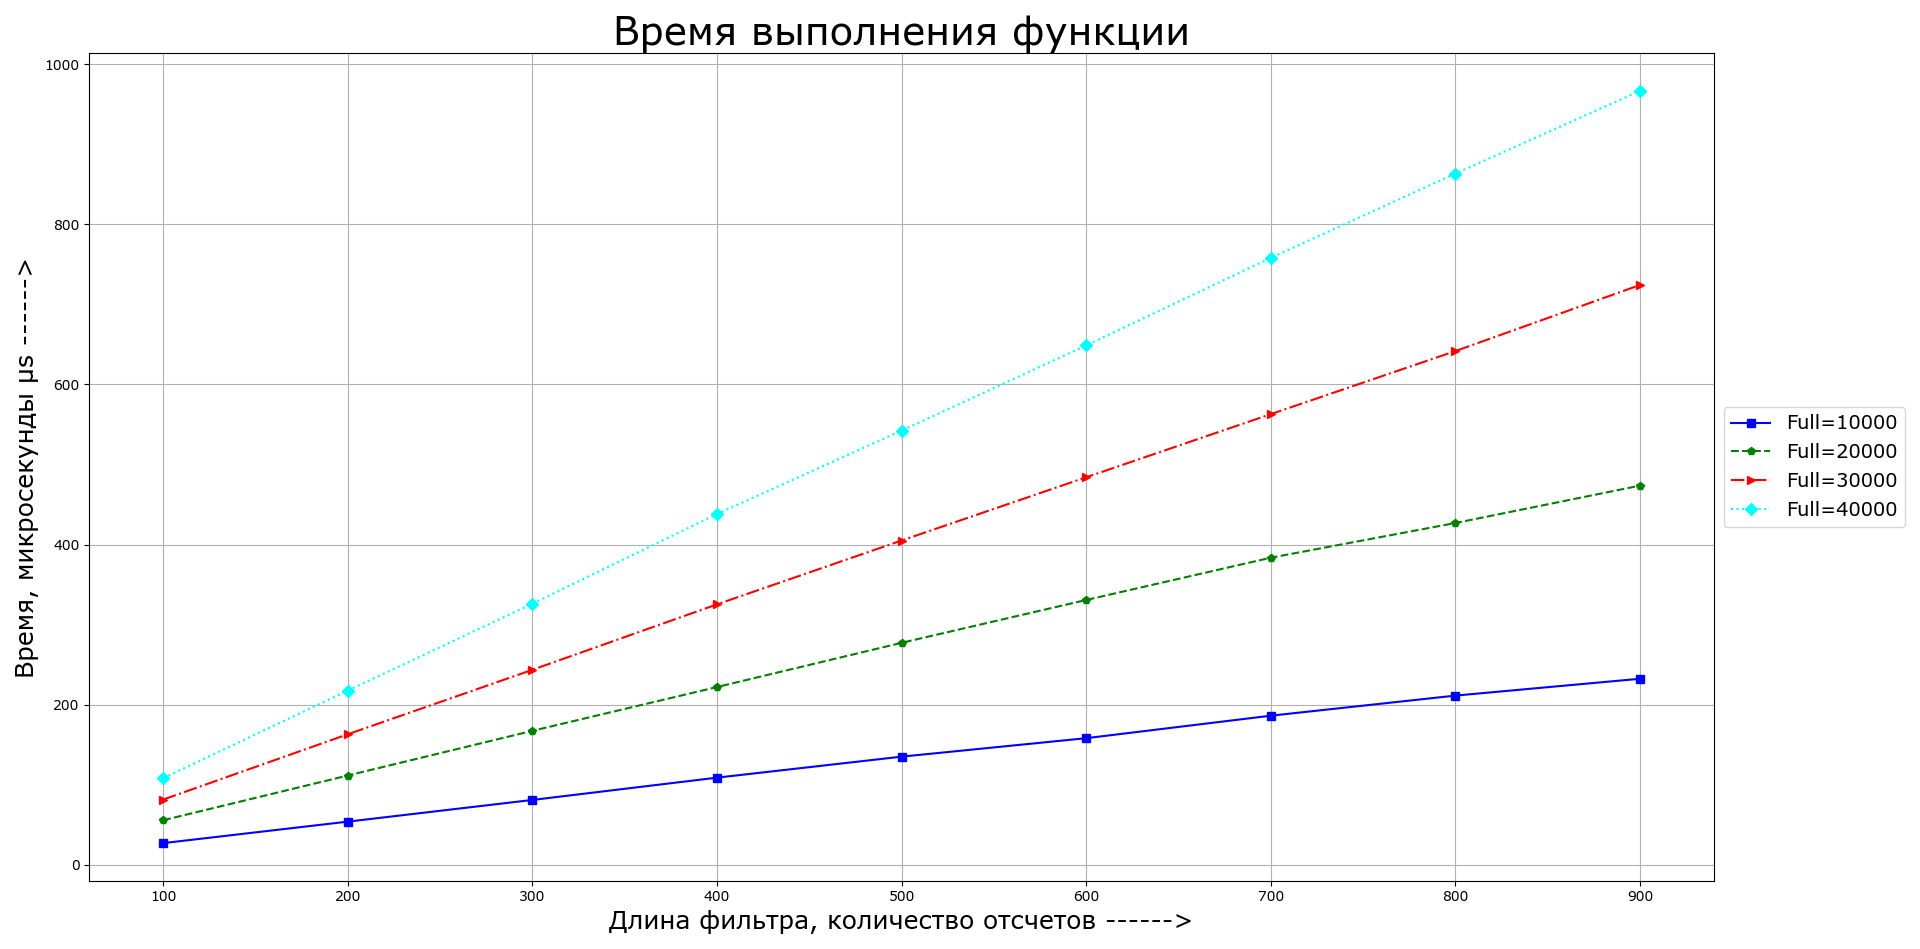
\includegraphics [scale=0.35] {convolution}
	\caption{Временные затраты на вычисление по алгоритму одномерной свертки на языке С (процессор Intel® Core™ $i5-3550$).}
	\label{img:convolution}
\end{figure}

В исследовании произведен анализ быстродействия реализаций алгоритмов одномерной свертки и цифровых фильтров. Для фильтрации  узкополосных сигналов требуются фильтры с импульсной характеристикой, содержащих большое число отчетов. 
В результате исследования была установлена необходимость минимизировать вычислительные затраты для цифровых фильтров с конечной импульсной характеристикой \ref{img:convolution}.
Для фильтрации  узкополосных сигналов, необходимо использовать быстрые алгоритмы, так.~как. они позволяют сократить количество операций. 


\section{Применение метода разложения двумерной свертки при реализации цифровых фильтров} \label{sec:ch3/sect4}
% Альтман Е. А., Захаренко Е. И., Васеева Т. В. Применение метода разложения двумерной свертки при реализации цифровых фильтров //Научный вестник Новосибирского государственного технического университета. – 2017. – №. 4. – С. 95-104.
В данной статье рассматривается вопрос вычислительной эффективности одной из базовых операций для алгоритмов обработки изображений и компьютерного зрения – фильтрации изображения \cite{Gonzalez2012digital}.
% 2. Гонсалес Р., Вудс Р. Цифровая обработка изображений. – 2012.
Под цифровой фильтрацией понимаются не только процедуры удаления шума или другой информации из сигнала, но и многие другие методы (изменение яркости, контрастности, выделение границ и~т.~д.), реализуемые с помощью математической операции двумерной свертки \cite{Rabiner1978theory, bluehut1989fast}.
% 3. Рабинер Л., Гоулд Б. Теория и применение цифровой обработки сигналов. – Рипол Классик, 1978.

% 4. Блейхут Р. Э. Быстрые алгоритмы цифровой обработки сигналов. – Мир, 1989.

При цифровой обработке сигналов часто применяются две схожие операции: (линейная) свертка (convolution) и корреляция (correlation) \cite{bluehut1989fast, Lukin2002Introduction}. Они имеют схожие формулы, и для их быстрого вычисления могут использоваться одни и те же методы. 
% 4. Блейхут Р. Э. Быстрые алгоритмы цифровой обработки сигналов. – Мир, 1989.

% 5. Лукин А. Введение в цифровую обработку сигналов //М.: МГУ. Лаборатория компьютерной графики и мультимедиа. – 2002.

Линейная двумерная дискретная свертка определяется следующей формулой \cite{decomposition_method_application2017}:
\begin{equation}
	\label{eq:equation3.5.1}
	CON_{j1,j2} = \sum_{i1 =0}^{n1-1} \sum_{i2 =0}^{n2-1} x_{i1,i2} \cdot y_{i1-j1,i2-j2}
\end{equation}

Далее для простоты изложения и обобщения будем использовать терминологию, применяемую при использовании свертки для вычисления цифровых фильтров. В этом контексте $n1$ и $n2$ – это длина ядра цифрового фильтра по первой и второй размерности соответственно, $x$ – ядро или импульсная характеристика цифрового фильтра, $y$ – отчеты входной последовательности (обрабатываемое изображение) и $CON$ – выходная последовательность фильтра (свертка входной последовательности с ядром фильтра). 

Дискретная корреляция двух последовательностей определяется следующей формулой: 
\begin{equation}
	\label{eq:equation3.5.2}
	COR_{j1,j2} = \sum_{i1 =0}^{n1-1} \sum_{i2 =0}^{n2-1} x_{i1,i2} \cdot y_{i1+j1,i2+j2}
\end{equation}

Для пояснения этой формулы также воспользуемся примером ее применения для обработки изображения. В этом контексте $x$ – это фрагмент изображения размером $ n1 \times n2 $, для которого рассчитывается корреляция; $y$ – область, с которой сравнивается фрагмент изображения, и $COR$ – корреляция.

Любую из приведенных операций можно свести к другой, инвертировав входные последовательности по всем размерностям. Это делает возможным применение одних и тех же алгоритмов для их выполнения. Однако имеются
отдельные аспекты применения этих операций при решении конкретных задач.

Во-первых, следует рассмотреть диапазоны, в которых берутся значения для переменных $j1$ и $j2$. Предположим, последовательность y имеет размер $m1 \times m2$. Для обеих рассматриваемых операций в зависимости от решаемой задачи может потребоваться найти результаты в диапазонах: 
\begin{enumerate}
	\item $0 \times 0: (m1 + n1 - 1) \times (m2 + n2 - 1)$;
	
	\item	$0 \times 0: n1 \times n2$;
	
	\item $0 \times 0: (m1 - n1 + 1) \times (m2 - n2 + 1)$. 
\end{enumerate}

В первом случае рассчитываются все возможные выходные значения, включая значения, для которых количество слагаемых в суммах будет меньше, чем $n1 \times n2$. Такой подход применяется в цифровых фильтрах (особенно в случае одномерных фильтров). Поскольку цифровая фильтрация является основным применением свертки, такой диапазон выходных значений часто указывается в определении свертки (хотя, строго говоря, это необязательное ограничение).

Во втором варианте диапазоны выходных значений используются не часто. Он удобен тем, что размер последовательности на выходе совпадает с размером последовательности на входе, и такие операции можно выполнять
последовательно.

В третьем варианте рассчитываются только выходные значения, для которых количество слагаемых в суммах будет равно $n1 \times n2$. Этот вариант позволяет сравнивать между собой значения без дополнительной нормировки, поэтому он является основным при вычислении корреляции.

Во-вторых, важным аспектом выполнения этих операций является соотношение между размерами последовательностей $x$ и $y$. При реализации цифровой фильтрации, как правило, $n1$ и $n2$ намного меньше $m1$ и $m2$. При вычислении корреляции эти величины чаще всего одного порядка.

В-третьих, следует учесть, что при решении отдельных задач одна из входных величин известна заранее, и над ней можно выполнить предварительные вычисления, не увеличивающие сложность основной операции.
Например, при цифровой фильтрации коэффициенты фильтра могут быть преобразованы в любую удобные форму на этапе разработки фильтра.

Перечисленные выше аспекты выполнения операций свертки и корреляции оказывают существенное влияние на реализацию операций. В частности, от этих аспектов зависит эффективность применения так называемых быстрых алгоритмов. 

В данной статье \cite{decomposition_method_application2017} рассматривается вопрос об эффективности применения подходов, предложенных для уменьшения количества вычислительных операций при реализации операции двумерной корреляции \cite{550562, altman2015fast}, для задачи выполнения двумерной фильтрации изображений (двумерной свертки).
% 6. Y. Naito, T. Miyazaki and I. Kuroda, "A fast full-search motion estimation method for programmable processors with a multiply-accumulator," 1996 IEEE International Conference on Acoustics, Speech, and Signal Processing Conference Proceedings, Atlanta, GA, USA, 1996, pp. 3221-3224 vol. 6, doi: 10.1109/ICASSP.1996.550562.

% 7. Альтман Е. А., Захаренко Е. И. Быстрый алгоритм вычисления двумерной корреляции для видеообработки //Доклады Томского государственного университета систем управления и радиоэлектроники. – 2015. – №. 2 (36).

Будем рассматривать три варианта вычисления двумерной свертки. Первый вариант – вычисление двумерной свертки непосредственно по формуле \ref{eq:equation3.5.1}. Второй вариант – использование предложенного в \cite{550562} алгоритма разложения двумерной свертки в несколько двумерных сверток меньших размеров. Третий вариант – использование быстрых алгоритмов одномерной свертки \cite{MOU1987377} для вычисления двумерной свертки.
% 6. Y. Naito, T. Miyazaki and I. Kuroda, "A fast full-search motion estimation method for programmable processors with a multiply-accumulator," 1996 IEEE International Conference on Acoustics, Speech, and Signal Processing Conference Proceedings, Atlanta, GA, USA, 1996, pp. 3221-3224 vol. 6, doi: 10.1109/ICASSP.1996.550562.

% 8. Mou Z. J., Duhamel P. Fast FIR filtering: algorithms and implementations //Signal Processing. – 1987. – Т. 13. – №. 4. – С. 377-384.

Отметим, что методы, основанные на разложении в свертки меньших размеров, имеют ограничение на размер сверток – ядро и входные данные должны иметь четное количество точек по каждой из размерностей. Это ограничение можно обойти с помощью комбинированного варианта вычисления свертки: для максимально возможного количества отчетов используется быстрый алгоритм вычисления, а оставшиеся вычисляются по определению.

Ввиду того, что типичные ядра цифровых фильтров обычно имеют небольшой размер, мы не будем рассматривать алгоритмы, основанные на различных быстрых алгоритмах преобразования сигналов (например, быстрое преобразование Фурье (БПФ)) \cite{Kalinovsky2016application, Digital_processing_Goldenberg_1985}.
% 9. Калиновский И. А., Спицын В. Г. Применение полиномиальных преобразований для быстрого вычисления двумерных сверток //Вычислительные методы и программирование: новые вычислительные технологии. – 2016. – Т. 17. – №. 3. – С. 197-203.

% 10. Гольденберг Л. М. и др. Цифровая обработка сигналов: Справочник. – Радио и связь, 1985.

Исходя из условий задачи примем, что предварительная обработка величины x не учитывается в общем числе операций и m значительно больше $n$.

При цифровой фильтрации изображений применяют разные способы обработки краев изображений, поэтому выбор диапазона выходных значений при фильтрации изображений является неоднозначным. Но, учитывая, что m зна-
чительно больше n, выбор этого диапазона незначительно скажется на относительной эффективности различных вариантов вычисления двумерной свертки. Для получения оценок сложности операций, не зависящих от диапа-
зона выходных значений, введем следующие обозначения: $l1$ – длина диапазона выходных значений по первой размерности, $l2$ – по второй.

При таких условиях для вычисления свертки по формуле \ref{eq:equation3.5.1} потребуется
$n1 \times n2 \times l1 \times l2$ умножений и $(n1 - 1) \times (n2 - 1) \times n2 \times l1 \times l2$ сложений, всего $(n1 \times n2 + (n1 - 1) \times (n2 - 1)) \times l1 \times l2$ операций.

Далее для сокращения размера формул примем следующие допущения.
Предположим, что размер входных данные достаточно велик, что можно пренебречь единицей в операциях сложения. Также примем, что $n = n1 = n2$,
$l = l1 = l2 и m = m1 = m2$. Как будет видно из дальнейшего изложения, такие

допущения не скажутся на окончательных выводах. Таким образом, сложность двумерной свертки приблизительно равна $2n^2 \times l^2$ операций или $2n^2$ операций на один отсчет (пиксель) входного сигнала.

В \cite{550562} для ускорения вычислений исходные данные разбиваются на части, в каждой из которых количество элементов в два раза меньше, чем в исходных данных по каждой из размерностей. При этом для удобства записи используется матричное представление данных. Преобразуем выражения из указанной статьи применительно к алгоритму двумерной свертки.
Введем промежуточные переменные:
% 6. Y. Naito, T. Miyazaki and I. Kuroda, "A fast full-search motion estimation method for programmable processors with a multiply-accumulator," 1996 IEEE International Conference on Acoustics, Speech, and Signal Processing Conference Proceedings, Atlanta, GA, USA, 1996, pp. 3221-3224 vol. 6, doi: 10.1109/ICASSP.1996.550562.
\begin{equation}
	\label{eq:equation3.5.3}
\hat{x}_{i1,i2} = [x_{i1,i2}, x_{i1+2,i2}, \cdots , x_{i1+n1-2,i2}]
\end{equation}

\begin{equation}
\label{eq:equation3.5.4}
\hat{y}_{i1,i2} = [y{i1,i2}, y_{i1+2,i2}, \cdots , y_{i1+m1-2,i2}]
\end{equation}

Обозначим части входных данных:
\begin{equation}
	\label{eq:equation3.5.5}
X_{i1,i2} = [\hat{x}_{i1,i2}, \hat{x}_{i1,i2+2}, \cdots , \hat{x}_{i1,i2+n2-2}] 
\end{equation}

\begin{equation}
	\label{eq:equation3.5.6}
	Y_{i1,i2} = [\hat{y}_{i1,i2}, \hat{y}_{i1,i2+2}, \cdots , \hat{y}_{i1,i2+m2-2}] 
\end{equation}

Используя введенные обозначения, формулу \ref{eq:equation3.5.1} можно переписать как:
\begin{equation}
	\label{eq:equation3.5.7}
CON_{j1,j2} = 
\begin{bmatrix}
CON_{j1,j2} \\ CON_{j1+1,j2} \\ CON_{j1,j2+1} \\ CON_{j1+1,j2+1}	
\end{bmatrix}
= \begin{bmatrix}
Y_{i1,i2} & Y_{i1-1,i2} & Y_{i1,i2-1} & Y_{i1-1,i2-1} \\
Y_{i1-1,i2} & Y_{i1-2,i2} & Y_{i1-1,i2-1} & Y_{i1-2,i2-1} \\
Y_{i1,i2-1}  & Y_{i1-1,i2-1}  & Y_{i1,i2-1} & Y_{i1-1,i2-2}  \\
Y_{i1-1,i2-1} & Y_{i1-2,i2-1} & Y_{i1-1,i2-2} & Y_{i1-2,i2-2} 	
\end{bmatrix}
\cdot
\begin{bmatrix}
X_{0,0} \\ X_{0,1} \\ X_{1,0} \\ X_{1,1}	
\end{bmatrix}		
\end{equation}

Обозначим:
\begin{equation}
	\label{eq:equation3.5.8}
A_0 = X_{0,0} - X_{1,0}.	
\end{equation}

\begin{equation}
	\label{eq:equation3.5.9}
	A_1 = X_{0,1} - X_{1,1}.	
\end{equation}

\begin{equation}
	\label{eq:equation3.5.10}
	B_{j1,j2} = Y_{j1,j2} - Y_{j1+1,j2}.	
\end{equation}

Тогда выражение \ref{eq:equation3.5.7} может быть разложено следующим образом:
\begin{equation}
\label{eq:equation3.5.11}
CON_{j1,j2} = 
\begin{bmatrix}
\left( {B_{j1,j2} + B_{j1,j2+1}} \right) X_{0,0} \\
\left( {B_{j1+1,j2} + B_{j1+1,j2+1}} \right) X_{1,0} \\
\left( {B_{j1,j2+1} + B_{j1,j2+2}} \right) X_{0,1} \\
\left( {B_{j1+1,j2+1} + B_{j1+1,j2+2}} \right) X_{1,1}
\end{bmatrix}
+
\begin{bmatrix}
-1 & 0 \\
0 & -1 \\
1 & 0  \\
0 & 1	
\end{bmatrix}
\cdot
\begin{bmatrix}
	B_{j1,j2+1} \left( {X_{0,0} - X_{0,1}} \right) \\
	B_{j1+1,j2+1} \left( {X_{1,0} - X_{1,1}} \right)	
\end{bmatrix}
+
\end{equation}

\begin{equation}
\label{eq:equation3.5.12}
+ 
\begin{bmatrix}
-1 & 0 \\
1 & 0 \\
0 & -1  \\
0 & 1	
\end{bmatrix}
\cdot
\begin{bmatrix}
\left(	{Y{j1+1,j2} + Y{j1+1,j2+1}} \right) \cdot A_0 \\
\left(	{Y{j1+1,j2+1} + Y{j1+1,j2+2}} \right) \cdot A_1	
\end{bmatrix}
+
\end{equation}

\begin{equation}
\label{eq:equation3.5.13}
+
\begin{bmatrix}
1 \\ -1 \\ -1 \\ 1
\end{bmatrix}
\cdot
Y{j1+1,j2+1}
\cdot
(A_0 - A_1)
\end{equation}

Как видно из формулы \ref{eq:equation3.5.11}, двумерная свертка сводится к девяти двумерным сверткам с размерами, меньшими в два раза по обеим размерностям.
Дополнительно к этим сверткам требуется выполнить еще несколько операций над матрицами, которые также меньше в два раза по обеим размерностям относительно исходных данных. Сложность этих сверток, если не применять дальнейшее рекурсивное разбиение на свертки меньшего размера, составит $\frac{9}{8n^2 × l^2}$ операций умножения и сложения.

В дополнительные операции входят действия над матрицами $X$ и $A$. Над ними выполняется пять сложений, но эти операции могут быть выполнены при разработке цифрового фильтра и не учитываться при подсчете сложности работы самого фильтра.
Также требуется вычислить шесть матриц $B$, два раза сложить матрицы
$Y$ и четыре раза сложить матрицы $B$. Для этого потребуется $\frac{12}{4m^2}$ операций.

На последнем этапе нужно собрать результаты сверток меньшей длины. По формуле для этого требуется выполнить $3 \times 4 = 12$ сложений матриц, но при сложении последних четверок матриц операции дважды повторяются, поэтому можно обойтись десятью сложениями. Сложность этих операций $\frac{10 }{4l^2}$.

Таким образом, сложность вычисления двумерной свертки при однократном разбиении на свертки меньшего размера составит примерно

$ \frac{9}{8n^2 \times l^2} + \frac{12}{4m^2} + \frac{10}{4l^2}$, еще более грубая оценка составит 
$\frac{9}{8n^2} \times l^2 + \frac{5}{2l^2}$ или $\frac{9}{8n^2} + \frac{5}{2}$ операций на один отсчет (пиксель) входного сигнала.

Метод использования одномерной свертки для вычисления двумерной зависит от ядра цифрового фильтра \cite{Digital_processing_Goldenberg_1985, gruzman2002digital}. 
% 11. Гольденберг Л. М. и др. Цифровая обработка сигналов: Справочник. – Радио и связь, 1985.
% 12. Грузман И. С. и др. Цифровая обработка изображений в информационных системах //Новосибирск: изд-во НГТУ. – 2002. – Т. 352. – С. 6.
Если ядро обладает свойством сепарабельности, то двумерная свертка сводится к двум одномерным сверткам. Это значительно сокращает количество требуемых операций, и при разработке фильтров разработчики стремятся получить именно такое ядро \cite{Huang1984fast}.
% 13. Хуанг Т. С. Быстрые алгоритмы в цифровой обработке изображений. – Издательство Pubmix. com, 1984.
Этот частный случай хорошо изучен, поэтому далее мы его рассматривать не
будем.

В общем случае ядро цифрового фильтра не является сепарабельным. В этом случае для ускорения двумерной свертки мы можем применить разложение, применяемое для разложения одномерной свертки \cite{MOU1987377} к внешней сумме двумерной свертки, вычисляя внутреннюю по обычной формуле.
% 8. Mou Z. J., Duhamel P. Fast FIR filtering: algorithms and implementations //Signal Processing. – 1987. – Т. 13. – №. 4. – С. 377-384.

Для оценки сложности этого варианта воспользуемся известной оценкой сложности одномерных цифровых фильтров \cite{haykin2005cocktail}. При однократном разбиении на свертки меньших размеров для вычисления одномерной свертки требуется $\frac{3}{4n}$ умножений и $ \frac{3}{4n}  + \frac{1}{2}$ сложений на один отчет входной последовательности или $\frac{3}{4n \times l}$ умножений и $ \frac{3}{ 4n \times l} +\frac{l}{2}$ сложений в целом. Умножим эти цифры на сложность внутренней суммы $n \times l$, получим
следующую оценку общего числа операций: $\frac{3}{2n^2 \times l^2} +\frac{n \times l^2}{2} $ или $\frac{3}{2n^2} + \frac{n^2}{2}$ операций на один отсчет (пиксель) входного сигнала.
% 14. Haykin S., Chen Z. The cocktail party problem //Neural computation. – 2005. – Т. 17. – №. 9. – С. 1875-1902.

Решая несложные уравнения, мы получим, что наименьшую сложность до $n \leq 1$ имеет метод полного перебора. Для n в диапазоне от $1$ до примерно $2,5$ наименьшую сложность имеет метод, основанный на разложении одномерной свертки. При $n > 2,5$ наименьшей сложностью обладает метод, основанный на разложении двумерной свертки.

Интерпретируя эти результаты, нужно учитывать, что они получены по 
приблизительным оценкам сложности алгоритмов, что алгоритмы, использующие разложения, можно применять не для всех значений n и что быстродействие алгоритмов при их практической реализации зависит не только от количества требуемых арифметических операций.

С учетом сказанного можно сделать вывод, что основанные на разложении быстрые алгоритмы вычисления двумерной свертки имеет смысл применять, начиная с размера ядра $4 \times 4$. Практически применяются ядра нечетных

размеров. Сокращение числа требуемых операций при применении разложения при ядре $5 \times 5$ составляет $16 \%$,$  7 \times 7 - 27 \% $, $9 \times 9 - 31 \%$. Ввиду сложности алгоритма разложения на свертки меньших размеров при практической реализации следует ожидать уменьшение выигрыша в быстродействии, тем
не менее следует сделать вывод, что рассмотренные в статье алгоритмы имеют практическую ценность для вычисления коротких сверток для ядер, начиная с размера $5 \times 5 $.


\section{Интерполированный алгоритм ДПФ} \label{sec:ch3/sect5}
Интерполированный алгоритм ДПФ (IpDFT -- Interpolated Discrete Fourier Transform) является одним из наиболее широко изученных методов оценки \cite{santamaria2000comparative, zhang2001algorithm, qian2007interharmonics, ferreira2005accurate, xie1996nonlinear, luo2015phase, jain1979high, grandke1983interpolation, andria1989windows, offelli1989interpolation, agrez2002weighted, jacobsen2007fast, belega2009multifrequency, belega2010accuracy, duda2011dft, schoukens1992interpolated}. 
% [156.-Santamaria I., Pantaleon C., Ibanez J. A comparative study of high-accuracy frequency estimation methods //Mechanical Systems and Signal Processing. – 2000. – Т. 14. – №. 5. – С. 819-834.]

% [157.-Zhang F., Geng Z., Yuan W. The algorithm of interpolating windowed FFT for harmonic analysis of electric power system //IEEE transactions on power delivery. – 2001. – Т. 16. – №. 2. – С. 160-164.]

%[158.-Qian H., Zhao R., Chen T. Interharmonics analysis based on interpolating windowed FFT algorithm //IEEE Transactions on Power Delivery. – 2007. – Т. 22. – №. 2. – С. 1064-1069.]

%[159.	Ferreira A., Sinha D. Accurate and robust frequency estimation in the ODFT domain //IEEE Workshop on Applications of Signal Processing to Audio and Acoustics, 2005. – IEEE, 2005. – С. 203-206.]

%[160.-Xie M., Adams D. F. A nonlinear finite element analysis for composite materials //Finite elements in analysis and design. – 1996. – Т. 22. – №. 3. – С. 211-223.]

%[161.-Luo J., Xie M. Phase difference methods based on asymmetric windows //Mechanical Systems and Signal Processing. – 2015. – Т. 54. – С. 52-67.]

%[162.-Jain V. K., Collins W. L., Davis D. C. High-accuracy analog measurements via interpolated FFT //IEEE Transactions on Instrumentation and Measurement. – 1979. – Т. 28. – №. 2. – С. 113-122.]

% [163.-Grandke T. Interpolation algorithms for discrete Fourier transforms of weighted signals //IEEE transactions on instrumentation and measurement. – 1983. – Т. 32. – №. 2. – С. 350-355.]

%[164.-Andria G., Savino M., Trotta A. Windows and interpolation algorithms to improve electrical measurement accuracy //IEEE Transactions on Instrumentation and Measurement. – 1989. – Т. 38. – №. 4. – С. 856-863.]

%[165.-Offelli C., Petri D. Interpolation techniques for real-time multifrequency waveform analysis //6th IEEE Conference Record., Instrumentation and Measurement Technology Conference. – IEEE, 1989. – С. 325-331.]

%[166.-Agrez D. Weighted multipoint interpolated DFT to improve amplitude estimation of multifrequency signal //IEEE Transactions on Instrumentation and Measurement. – 2002. – Т. 51. – №. 2. – С. 287-292.]

%[167.-Jacobsen E., Kootsookos P. Fast, accurate frequency estimators [DSP Tips & Tricks] //IEEE Signal Processing Magazine. – 2007. – Т. 24. – №. 3. – С. 123-125.]

%[168.	Belega D., Dallet D. Multifrequency signal analysis by interpolated DFT method with maximum sidelobe decay windows //Measurement. – 2009. – Т. 42. – №. 3. – С. 420-426.]

%[169.-Belega D., Dallet D., Petri D. Accuracy of sine wave frequency estimation by multipoint interpolated DFT approach //IEEE Transactions on Instrumentation and Measurement. – 2010. – Т. 59. – №. 11. – С. 2808-2815.]

%[170.-Duda K. DFT interpolation algorithm for Kaiser–Bessel and Dolph–Chebyshev windows //IEEE Transactions on Instrumentation and Measurement. – 2011. – Т. 60. – №. 3. – С. 784-790.]

%[171.-Schoukens J., Pintelon R., Van Kamme H. The interpolated fast Fourier transform: A comparative study //[1991] Conference Record. IEEE Instrumentation and Measurement Technology Conference. – IEEE, 1991. – С. 358-364.]


Рассмотрим непрерывный сигнал с аддитивным белым шумом:
\begin{equation}
	\label{eq:$x(t)$}
	x(t) = A_0 \cos \big( 2 \pi f_0 t + \theta_0 + e(t)\big) 
\end{equation}

где $A_0$ -- амплитуда;

$f_0$ -- частота;

$\theta_0$ -- фазовый угол;

$t$ -- время;

$e(t)$ -- белый шум. 

Частота $f_s$ с интервалом $N\bigtriangleup t$, где $\bigtriangleup t = \cfrac{1}{f_s}$, $N$ -- отчеты.

По теореме Котельникова (в зарубежной литературе теорема Найквиста -- Шеннона или теорема отчетов) непрерывные и дискретные сигналы $x(t)$ состоящих из частот ($0$ до $f_0$) можно передавать с любой точностью при помощи чисел, следующих друг за другом через $\frac{1}{2f_0}$. 

\begin{equation}
	\label{eq:$x(n)$}
	x(n) = A_0 \cos(2 \pi \frac{f_0}{f_s} n + \theta_0) + e(n), n = 0,1, \cdots , N-1
\end{equation}

По теореме Котельникова, $f_s$ больше $2f_0$. Разрешающая способность по частоте $\bigtriangleup f = \cfrac{f_s}{N}$ определяется:

\begin{equation}
	\label{eq:equation14}
	\frac{f_0}{f_s}=\frac{\lambda_0}{N}
\end{equation}

$\lambda_0$ -- количество циклов или нормированная частота.


Умножим отчеты сигнала $x(n)$ на значение окна данных $\omega(n)$.

\begin{equation}
	\label{eq:equation15}
	x_\omega(n)=A_0 \cos(\frac{2 \pi \lambda_0 n}{N}+\theta_0)\omega(n)
\end{equation}

ДПФ взвешенного сигнала может быть вычислена путем:

\begin{equation}
	\label{eq:equation16}
	X_\omega(k) = \sum_{n=0}^{N-1} x_\omega(n) e^{-j \frac{2 \pi}{N}nk}
\end{equation}

Применение \labelcref{eq:equation16} к отчетам в \labelcref{eq:equation15} дает вид:

\begin{equation}
	\label{eq:equation17}
	X_\omega(k) = \frac{A_0}{2} e^{j\phi_0}W_N(k-\lambda_0)+\frac{A_0}{2}e^{j\phi_0}W_N(k+\lambda_0)
\end{equation}

где $W_N (k)$ -- дискретное временное преобразование Фурье (DTFT-- Discrete time Fourier transform) весовой функции. 

Нормированная частота $\lambda_0$ находится между двумя самыми большими спектральными линиями. Следовательно, $\lambda_0$  может быть записано с целой частью $l_\omega$ и дробной частью $\delta_\omega$ $(-0,5<\delta_{\omega}\leq0,5)$.

\begin{equation}
	\label{eq:equation18}
	\lambda_0 = l_\omega + \delta_\omega
\end{equation}

Целая часть $l_\omega$ может быть определена с помощью отношения сигнал/шум (SNR -- signal-to-noise ratio) превышает пороговое значение (приблизительно от -$18$ до –$20$ дБ) \cite{rife1974single}. 

Подстановка формулы \labelcref{eq:equation18} в \labelcref{eq:equation17}:
\begin{equation}
	\label{eq:equation19}
	\left|{X_\omega(l_\omega)} \right| = \frac{A_0}{2} \left| e^{j\phi_0}W_N(- \delta_\omega) +e^{j\phi_0}W_N(2l_\omega+\delta_\omega) \right| 
\end{equation}

Параметр $\alpha$ зависит только от выбранного окна и отклонения частоты $\delta_{\omega}$. 

\begin{equation}
	\label{eq:equation20}
	\delta_\omega = g(\alpha)
\end{equation}

Для максимальных окон распада боковых лепестков $\delta_{\omega}$ запишем как функцию от $\alpha$ в простой форме \cite{zhang2001algorithm, qian2007interharmonics, xie1996nonlinear, luo2015phase, belega2009multifrequency, belega2010accuracy}. Для других окон предлагается решение полиномиальной аппроксимации \cite{duda2011dft}. 

Рассмотрим алгоритм техники заполнения нулями. Заполнение нулями -- это метод, определяемый как добавление нулевых значений к отчетам до вычисления ДПФ. Добавленные нулевые значения обрабатываются как дополнительные отчеты, поэтому увеличивают время измерения \labelcref{eq:equation21}:

\begin{equation}
	\label{eq:equation21}
	x_{ap}(n)=
	\begin{cases}
		x_{\omega}, \leq n < N
		\\ 0, N \leq n < MN
	\end{cases}
\end{equation}

где $(M-1) \cdot N$ -- добавление нулевых значений.

Соответственно, дискретный спектр расширяется. Эта процедура приводит к более точной выборке спектра сигнала, потому что вместо $N$ спектральных отчетов $M \cdot N$. Добавление нулевых значений и вычисление более длинного ДПФ действительно увеличивает количество точек в частотной области \cite{dorf2006circuits}.

Алгоритм техники заполнения нулями не влиет на параметры спектра (отношение сигнал/шум, спектральная утечка).  Коэффициенты ДПФ по \labelcref{eq:equation21}:

\begin{equation}
	\label{eq:equation22}
	X(N)= \sum_{n=0}^{MN-1} x_{ap}(n) e^{-j \frac{2 \pi}{N}\cdot \frac{k}{M} \cdot n}, 0\leq k \leq MK-1
\end{equation}
По сравнению с \labelcref{eq:equation16} получается:

\begin{equation}
	\label{eq:equation23}
	X(k)= X_\omega \left( {\frac{k}{M}}\right)  \end{equation}
Соответственно, \labelcref{eq:equation19} можно переформулировать как:

\begin{equation}
	\label{eq:equation24}
	\left| {X(l)} \right|   = \frac{A_0}{2}\left| {e^{j\phi_0}W_N(-\delta)+e^{-j\phi_0}W_N \left(\frac{2l}{M}+\delta \right)} \right|,
\end{equation}

где $l$ и $\hat{\delta}
\left( {\delta= \frac{\hat{\delta}}{M}}\right) $
часть для $M\lambda_0$. Точно так же $l$ возвращается максимальной процедурой поиска X(k). На этом этапе три крупнейших линии $X(k)$ даны $\left| {X(l)} \right|$,$\left| {X(l+1)} \right|$ а также $\left|{X(l-1)}\right|$.

Рассмотрим алгоритм интерполяции для окна Хеннинга с техникой заполнения нулями.
Если $\lambda_0$ удовлетворяет $5<\lambda_0$ , а также $\lambda_0 < \frac{N}{2}-5$, тогда помехи от второго слагаемого могут быть минимальными и ими можно пренебречь. Поэтому \labelcref{eq:equation24} сводится к:
\begin{equation}
	\label{eq:equation25}
	\left| {X(l)} \right| \cong \frac{A_0}{2}\left| {W_N(-\delta)} \right|,
\end{equation}

Если $\left| {X(l)} \right| \cong \frac{A_0}{2}\left| {W_N(\varepsilon -\delta)} \right|$ и $\left| {X(l-1)} \right| \cong \frac{A_0}{2} \left| {W_N(\varepsilon +\delta)} \right|$, где $\varepsilon=\frac{1}{M}$. 

Для окна Хеннинга (Hanning window), $W_N (k) \cong \frac{sin(\pi k)}{h(k)}$,
$h(k) = 2 \pi k (1-k^2)$ \cite{xie1996nonlinear}
%[160.	Xie M., Adams D. F. A nonlinear finite element analysis for composite materials //Finite elements in analysis and design. – 1996. – Т. 22. – №. 3. – С. 211-223.]

\begin{equation}
	\label{eq:equation26}
	\left| {X(l)} \right| \cong \frac{A_0}{2} \frac{\sin{(\pi \delta)} }{h(\delta)} ,
\end{equation}

\begin{equation}
	\label{eq:equation27}
	\left| {X(l+1)} \right| \cong \frac{A_0}{2} \frac{\sin{(\pi \varepsilon - \pi \delta)} }{h(\varepsilon - \delta)} ,
\end{equation}

\begin{equation}
	\label{eq:equation28}
	\left| {X(l+1)} \right| \cong \frac{A_0}{2} \frac{\sin{(\pi \varepsilon + \pi \delta)} }{h(\varepsilon + \delta)}
\end{equation}

Объединим уравнения вместе (\labelcref{eq:equation27} и \labelcref{eq:equation28}):

\begin{equation}
	\label{eq:equation29}
	h(\varepsilon+\delta)\left|{X(l-1)} \right| - h(\varepsilon-\delta) \left|{X(l+1)} \right| \cong A_0 \sin{(\pi \delta)} \cos{(\pi \varepsilon)}
\end{equation}

Дальнейшее объединение \labelcref{eq:equation26} и \labelcref{eq:equation29}

\begin{equation}
	\label{eq:equation30}
	h(\delta+\varepsilon)\left|{X(l-1)} \right| - h(\delta - \varepsilon) \left|{X(l+1)} \right| \cong 2 \left|{X(l)} \right| h(\delta) \cos{(\pi \varepsilon)}
\end{equation}

Теперь введем две переменные $\gamma_1$,$\gamma_2$ определяются как:

\begin{equation}
	\label{eq:equation31}
	\gamma_1 = \frac{\left| X(l-1)\right|}{\left| X(l)\right|}
\end{equation}

\begin{equation}
	\label{eq:equation32}
	\gamma_1 = \frac{\left| X(l+1)\right|}{\left| X(l)\right|}
\end{equation}

Для простоты и краткости будем использовать знак $«=»$ в \labelcref{eq:equation30}, вместо $\cong$. Но отношение аппроксимации остаются. 

\begin{equation}
	\label{eq:equation33}
	h(\delta +\varepsilon)\gamma_1 - h(\delta -\varepsilon)\gamma_2 = 
	2h(\delta) \cos(\pi \varepsilon) 
\end{equation}

При условии $h(\delta +\varepsilon)$,$h(\delta -\varepsilon)$ получаем:

\begin{equation}
	\label{eq:equation34}
	{a \delta}^3 + {b \delta}^2 + c \delta + d = 0, 
\end{equation}

где $a = 2 \cos(\pi \varepsilon)-(\gamma_1 + \gamma_2)$;

$b = -3(\gamma_1 - \gamma_2)\varepsilon$;

$c = \left( \gamma_1 + \gamma_2 - \frac{2 \cos(\pi \varepsilon)}{1-3\varepsilon^2}
\right) \left( {1-3\varepsilon^2} \right) $;

$d = ( \gamma_1 - \gamma_2)(\varepsilon - \varepsilon^3)$

\begin{equation}
	\label{eq:equation35}
	g(\delta) = {a \delta}^3 + {b \delta}^2 + c \delta + d
\end{equation}

Можно доказать, что $g(-1)>0$,$g(-0,5)<0$,$g(0,5)>0$,$g(1)<0$ 

\begin{equation}
	\label{eq:equation36}
	\gamma_1 = \frac{\left| X(l-1)\right|}{\left| X(l)\right|} = \frac{\sin({\pi \varepsilon + \pi \delta})}{h(\varepsilon + \delta)} \cdot \frac{h(\delta)}{\sin(\pi \delta)}
\end{equation}

\begin{equation}
	\label{eq:equation37}
	\gamma_2 = \frac{\left| X(l+1)\right|}{\left| X(l)\right|} = \frac{\sin({\pi \varepsilon - \pi \delta})}{h(\varepsilon - \delta)} \cdot \frac{h(\delta)}{\sin(\pi \delta)}
\end{equation}

где $\delta \in[-0.5,0.5]$ а также $\varepsilon\in[0,0.5]$. Согласно формуле \labelcref{eq:equation35}

\begin{equation}
	\label{eq:equation38}
	f(0,5) = -\frac{3}{4} \cos(\pi \varepsilon) + \frac{(1-4 \varepsilon^2)}{8} \left[ {\gamma_1 (3+2 \varepsilon)+\gamma_2 (3-2 \varepsilon)}\right] 
\end{equation}

\begin{equation}
	\label{eq:equation39}
	f(-0,5) = +\frac{3}{4} \cos(\pi \varepsilon) + \frac{(1-4 \varepsilon^2)}{8} \left[ {\gamma_1 (3-2 \varepsilon)+\gamma_2 (3+2 \varepsilon)}\right] 
\end{equation}

\begin{equation}
	\label{eq:equation40}
	f(1) = -\gamma_1 \varepsilon(\varepsilon+1)(\varepsilon + 2) + \gamma_2 \varepsilon(\varepsilon-1)(\varepsilon - 2)
\end{equation}

\begin{equation}
	\label{eq:equation41}
	f(-1) = -\gamma_1 \varepsilon(\varepsilon-1)(\varepsilon - 2) + \gamma_2 \varepsilon(\varepsilon+1)(\varepsilon + 2)
\end{equation}

Определяем $p(\delta)$:

\begin{equation}
	\label{eq:equation42}
	p(\delta) = \gamma_1 (3+2\varepsilon) + \gamma_2 (3-2\varepsilon)
\end{equation}

Определяем $q(\delta)$:
\begin{equation}
	\label{eq:equation43}
	q(\delta) = \gamma_1 (3-2\varepsilon) + \gamma_2 (3+2\varepsilon)
\end{equation}

$p(\delta)$ является монотонно возрастающей функцией. Поэтому:
\begin{equation}
	\label{eq:equation44}
	p_{min}(\delta) = p(\delta = 0,5) = \frac{6 \cos(\pi  \varepsilon)}{1-4\varepsilon ^2}
\end{equation}

также
\begin{equation}
	\label{eq:equation45}
	q_{min}(\delta) = q(\delta = -0,5) = \frac{6 \cos(\pi  \varepsilon)}{1-4\varepsilon ^2}
\end{equation}

Тогда
\begin{equation}
	\label{eq:equation46}
	f(0,5) > -\frac{3}{4} \cos (\pi \varepsilon) + \frac{(1-4 \varepsilon ^2)}{8} p_{min} (\delta) = - \frac{3}{4} \cos(\pi \varepsilon) + \frac{3 \ cos(\pi \varepsilon)}{4} = 0 
\end{equation}

\begin{equation}
	\label{eq:equation47}
	f(-0,5) < \frac{3}{4} \cos (\pi \varepsilon) + \frac{(1-4 \varepsilon ^2)}{8} q_{min} (\delta) = + \frac{3}{4} \cos(\pi \varepsilon) - \frac{3 \ cos(\pi \varepsilon)}{4} = 0 
\end{equation}

Определим:
\begin{equation}
	\label{eq:equation48}
	u(\varepsilon, \gamma) = \frac{f(1)}{\varepsilon \gamma_1} = (\varepsilon ^2 + 2) (\gamma - 1) - 3\varepsilon (\gamma + 1)
\end{equation}

\begin{equation}
	\label{eq:equation49}
	\nu(\varepsilon, \gamma) = \frac{f(-1)}{\varepsilon \gamma_1} = (\varepsilon ^2 + 2) (\gamma - 1) + 3\varepsilon (\gamma + 1)
\end{equation}

$\gamma = \frac{\gamma_1}{\gamma_2}$

\begin{equation}
	\label{eq:equation50}
	u'_{\gamma}(\varepsilon, \gamma) = \varepsilon^2 - 3\varepsilon + 2 = (\varepsilon - 2)(\varepsilon -1) >0
\end{equation}

\begin{equation}
	\label{eq:equation51}
	{\nu}'_\gamma
	(\varepsilon, \gamma) = \varepsilon^2 + 3\varepsilon + 2 = (\varepsilon + 2)(\varepsilon + 1) >0
\end{equation}


\begin{equation}
	\label{eq:equation52}
	u _{max}(\varepsilon, \gamma) =
	\left( {\varepsilon^2+2} \right) 
	\left( {\frac{1,5+\varepsilon}{1,5-\varepsilon}-1} \right) - 3 \varepsilon 
	\left( {\frac{1,5+\varepsilon}{1,5-\varepsilon}+1} \right) = \frac{\varepsilon}{1,5-\varepsilon}(2\varepsilon^2 - 5) < 0
\end{equation}

\begin{equation}
	\label{eq:equation53}
	\nu _{min}(\varepsilon, \gamma) =
	\left( {\varepsilon^2+2} \right) 
	\left( {\frac{1,5-\varepsilon}{1,5+\varepsilon}-1} \right) - 3 \varepsilon 
	\left( {\frac{1,5-\varepsilon}{1,5+\varepsilon}+1} \right) = \frac{\varepsilon}{1,5-\varepsilon}(5-2\varepsilon^2) > 0
\end{equation}

Соответственно:

\begin{equation}
	\label{eq:equation54}
	f(1) = u(\varepsilon, \gamma)(\varepsilon \gamma_1) <0
\end{equation}

\begin{equation}
	\label{eq:equation55}
	f(-1) = \nu(\varepsilon, \gamma)(\varepsilon \gamma_1) > 0
\end{equation}

Согласно исследованию в \cite{nickalls1993new}, корни можно выразить:

%[174.	Nickalls R. W. D. A new approach to solving the cubic: Cardan’s solution revealed //The Mathematical Gazette. – 1993. – Т. 77. – №. 480. – С. 354-359.]

\begin{equation}
	\label{eq:equation56}
	\delta_1 = 
	\delta_0 + 2 \sigma \cos \left({\frac{2 \pi}{3}} + \varphi  \right) 
\end{equation}

\begin{equation}
	\label{eq:equation57}
	\delta_2 = 
	\delta_0 + 2 \sigma \cos \left({\frac{2 \pi}{3}} - \varphi  \right) 
\end{equation}

\begin{equation}
	\label{eq:equation58}
	\delta_3 = 
	\delta_0 + 2 \sigma \cos (\varphi) 
\end{equation}

$\delta_0 = \frac{-a}{3b};$

$\sigma = \sqrt{\frac{b^2 - 3ac}{9a^2}}$

$\cos(3 \varphi) = - g \left( {\frac{\delta_0}{p}}
\right) $

$p = -a \delta_0 ^3$

$\delta_1$ и $\delta_3$ выходят за пределы определенного диапазона $(-0,5;0,5]$. Таким образом, единственным решением является $\delta_2 $. Получаем:

\begin{equation}
	\label{eq:equation59}
	\hat{\delta} = \delta_2 + \delta_0 + 2 \sigma \cos \left({\frac{2 \pi}{3} - \varphi} \right) 
\end{equation}

Рассмотрим расширение на другие классические окна .

Расширим интерполяцию для других классических окон, используя метод подгонки основного лепестка. 

\begin{equation}
	\label{eq:equation60}
	S(k) = [W_C (k)]^q - W_H (k)
\end{equation}

где $W_C (k)$ -- обозначает нормализованный спектр любого классического окна;

$W_H (k)$ -- обозначает нормализованный спектр окна Хеннинга;

$q = \frac{S L_{Han}}{S L_\omega(n)}$

$S L_{Han}$ и $S L_\omega(n)$ -- представляют собой убывающие потери $SL$ окна Хеннинга.

Можно определить, что $|S(k)|$ очень мало 
для большинства классических окон, если $k$ находится в диапазоне  $(-0,5;0,5]$. 
Например, максимальное значение $|S(k)|$ равняется $10-5$ для окна Хемминга(Hamming window) и $10^-4$ для окна Блэкмена (Blackman window).
Означает, что $[W_C (k)]^q$, а также $W_H (k)$ хорошо сочетаются друг с другом в середине их основных лепестков. 
Подразумевается, что вышеуказанный алгоритм интерполяции может быть расширен для классических окон, пока $[W_C (k)]^q$ используется $k$ и ограничен в диапазоне $[-0,5;0,5]$. 
С техникой заполнения нулями $(M\geq3)$, три самые большие спектральные линии, которые используются в алгоритме интерполяции, легко удовлетворяют требованию. Для большого $M$, погрешность оценки будет уменьшаться как в шуме, так и в ситуации без шума. Однако улучшение не ясно, когда $(M>5)$. С другой стороны, объем расчета увеличится из-за добавленного нуля. Следовательно, учитывая объем вычислений и алгоритм БПФ для radix-2, часто выбираем $(M=4)$ для практических измерений.

Согласно определению в уравнениях \labelcref{eq:equation31} и \labelcref{eq:equation32}, имеем

\begin{equation}
	\label{eq:equation62}
	\gamma_1 = \frac{\left| X(l-1)\right|}{\left| X(l)\right|} = \frac{\sin \pi({\delta + \varepsilon})}{\sin \pi \delta} \cdot \frac{h(\delta)}{h(\delta + \varepsilon)}
\end{equation}

\begin{equation}
	\label{eq:equation63}
	\gamma_2 = \frac{\left| X(l+1)\right|}{\left| X(l)\right|} = \frac{\sin \pi({\delta - \varepsilon})}{\sin \pi \delta} \cdot \frac{h(\delta)}{h(\delta - \varepsilon)}
\end{equation}

\begin{equation}
	\label{eq:equation64}
	\gamma = \frac{\left| X(l+1)\right|}{\left| X(l-1)\right|} = \frac{\sin \pi({\delta - \varepsilon})}{\sin \pi ({\delta + \varepsilon})} \cdot \frac{h({\delta + \varepsilon})}{h(\delta - \varepsilon)}
\end{equation}

Знаем $\gamma_1$, является монотонно убывающей функцией и $\gamma_2$, $\gamma$ является монотонно возрастающей функцией в зависимости от $\delta$ в диапазоне $[-0.5;0.5]$. Итак, можем получить

\begin{equation}
	\label{eq:equation65}
	\gamma_{1 max} = \gamma_1 (\delta = - 0,5) = \frac{3 \cos \pi \varepsilon}{(1 + 2 \varepsilon)(1 - 2 \varepsilon)(3 - 2 \varepsilon)}
\end{equation}

\begin{equation}
	\label{eq:equation66}
	\gamma_{1 min} = \gamma_1 (\delta = 0,5) = \frac{3 \cos \pi \varepsilon}{(1 + 2 \varepsilon)(1 - 2 \varepsilon)(3 + 2 \varepsilon)}
\end{equation}

\begin{equation}
	\label{eq:equation67}
	\gamma_{2 max} = \gamma_2 (\delta = 0,5) = \frac{3 \cos \pi \varepsilon}{(1 + 2 \varepsilon)(1 - 2 \varepsilon)(3 - 2 \varepsilon)}
\end{equation}

\begin{equation}
	\label{eq:equation68}
	\gamma_{2 min} = \gamma_2 (\delta = -0,5) = \frac{3 \cos \pi \varepsilon}{(1 + 2 \varepsilon)(1 - 2 \varepsilon)(3 + 2 \varepsilon)}
\end{equation}

\begin{equation}
	\label{eq:equation69}
	\gamma_{max} = \gamma(\delta = 0,5) = \frac{1,5+ \varepsilon}{1,5 - \varepsilon}
\end{equation}

\begin{equation}
	\label{eq:equation70}
	\gamma_{min} = \gamma(\delta = -0,5) = \frac{1,5 - \varepsilon}{1,5 + \varepsilon}
\end{equation}

Согласно бесконечному представлению Эйлера функции синуса:

\begin{equation}
	\label{eq:equation71}
	\sin \pi \delta = \pi \delta \prod\limits_{n = 1}^\infty \left( 1- \frac{\delta^2}{n^2} \right) 
\end{equation}

\begin{equation}
	\label{eq:equation72}
	E(\delta) = \frac{\sin(\pi \delta) }{h(\delta)} = \frac{\pi \delta \prod\limits_{n = 1}^\infty \left( 1- \frac{\delta^2}{n^2}\right)}{\pi \delta (1 - \delta^2)} = \prod\limits_{n = 2}^\infty \left( 1 - \frac{\delta^2}{n^2}\right) \geq 0 
\end{equation}

Находим производную $E(\delta)$:     

\begin{equation}
	\label{eq:equation73}
	E'(\delta) = E(\delta)L(\delta)
\end{equation}

\begin{equation}
	\label{eq:equation74}
	L(\delta) = \sum_{n=2}^{\infty} \frac{-2 \delta}{n^2 - \delta^2} = \sum_{n=2}^{\infty} \left(  \frac{1}{n + \delta} -  \frac{1}{n - \delta} \right) 
\end{equation}

\begin{equation}
	\label{eq:equation75}
	D(\delta) = \frac{E(\delta)}{E(\delta + \epsilon)} = \frac{\prod\limits_{n = 2}^\infty \left( 1 - \frac{\delta^2}{n^2} \right) }{\prod\limits_{n = 2}^\infty \left( \frac{1 - (\delta + \epsilon)^2}{n^2}\right)} = \prod\limits_{n = 2}^\infty \frac{n^2 - \delta^2}{n^2 - (\delta + \epsilon)^2}
\end{equation}

\begin{equation}
	\label{eq:equation76}
	D'(\delta) = \frac{E(\delta)L(\delta)E(\delta + \epsilon) - E(\delta)E(\delta + \epsilon)L(\delta + \epsilon)}{E^2 (\delta + \epsilon)} = \frac{E(\delta) [L(\delta) - L(\delta + \epsilon)])}{E(\delta + \epsilon)}
\end{equation}

\begin{equation}
	\label{eq:equation77}
	L(\delta) - L(\delta + \epsilon) = \sum_{n=2}^{\infty} \left(  \frac{\epsilon}{(n + \delta)(n + \delta + \epsilon)} + \frac{\epsilon}{(n - \delta)(n - \delta - \epsilon)} \right) > 0
\end{equation}

\begin{equation}
	\label{eq:equation78}
	D'(\delta) > 0 
\end{equation}

$D(\delta)$ -- монотонно возрастающая функция в зависимости от $\delta$, $\frac{1}{D(\delta)}$ -- монотонно убывающая функция. 

На основании уравнения \labelcref{eq:equation72} $\gamma_1, \gamma_2$ могут быть представлены:

\begin{equation}
	\label{eq:equation79}
	\gamma_1 = \frac{E(\delta + \epsilon)}{E(\delta)} 
\end{equation}

\begin{equation}
	\label{eq:equation80}
	\gamma_2 = \frac{E(\delta - \epsilon)}{E(\delta)} 
\end{equation}

\begin{equation}
	\label{eq:equation81}
	p(\delta) = \frac{[E(\delta + \epsilon)(3 + 2 \epsilon) + E(\delta - \epsilon)(3 - 2 \epsilon)]}{E(\delta)}
\end{equation}

\begin{equation}
	\label{eq:equation82}
	q(\delta) = \frac{[E(\delta + \epsilon)(3 - 2 \epsilon) + E(\delta - \epsilon)(3 + 2 \epsilon)]}{E(\delta)}
\end{equation}

\begin{equation}
	\label{eq:equation83}
	p'(\delta) = \frac{H_{p}(\delta, \epsilon)}{E(\delta)}
\end{equation}

\begin{equation}
	\label{eq:equation84}
	q'(\delta) = \frac{H_{q}(\delta, \epsilon)}{E(\delta)}
\end{equation}

Где $H_{p}(\delta, \epsilon)$ и $H_{q}(\delta, \epsilon)$ соответственно:

\begin{equation}
	\label{eq:equation85}
	H_{p}(\delta, \epsilon) = E(\delta + \epsilon)(3 + 2 \epsilon) [L (\delta + \epsilon) - L(\delta)] + E(\delta - \epsilon)(3 - 2\epsilon) [L(\delta - \epsilon) - L(\delta)]
\end{equation}

\begin{equation}
	\label{eq:equation86}
	H_{q}(\delta, \epsilon) = E(\delta + \epsilon)(3 - 2 \epsilon) [L (\delta + \epsilon) - L(\delta)] + E(\delta - \epsilon)(3 + 2\epsilon)[L(\delta - \epsilon) - L(\delta)]
\end{equation}

\begin{equation}
	\label{eq:equation87}
	H_{p}(\delta, \epsilon) + H_{p}(- \delta, \epsilon) = 4 \epsilon E (\delta + \epsilon) [L(\delta + \epsilon) - L(\delta)] + 4 \epsilon E (\delta - \epsilon)[L(\delta) - L (\delta - \epsilon)] 
\end{equation}

\begin{equation}
	\label{eq:equation88}
	H_{q}(\delta, \epsilon) + H_{q}(- \delta, \epsilon) = - 4 \epsilon E (\delta + \epsilon) [L(\delta + \epsilon) - L(\delta)] - 4 \epsilon E (\delta - \epsilon)[L(\delta) - L (\delta - \epsilon)]  
\end{equation}

Если $L (\delta - \epsilon) - L(\delta) < 0$ и $L(\delta) - L(\delta - \epsilon) < 0$, то:

\begin{equation}
	\label{eq:equation89}
	H_{p}(\delta, \epsilon) + H_{p}(- \delta, \epsilon) < 0  
\end{equation}

\begin{equation}
	\label{eq:equation90}
	H_{q}(\delta, \epsilon) + H_{q}(- \delta, \epsilon) > 0  
\end{equation}

\begin{equation}
	\label{eq:equation91}
	H_{p}(\delta, \epsilon) < 0
\end{equation}

\begin{equation}
	\label{eq:equation92}
	H_{q}(\delta, \epsilon) > 0
\end{equation}

\begin{equation}
	\label{eq:equation93}
	p'(\delta) = \frac{H_{p}(\delta, \epsilon)}{E(\delta)} < 0
\end{equation}

\begin{equation}
	\label{eq:equation94}
	q'(\delta) = \frac{H_{q}(\delta, \epsilon)}{E(\delta)} > 0
\end{equation}

где $p(\delta)$ -- убывающая функция;

$\delta$ -- убывающая функция;

$q(\delta)$ -- возрастающая функция.

\begin{equation}
	\label{eq:equation95}
	I(\delta, \epsilon) = \frac{E(\delta - \epsilon)}{E(\delta + \epsilon)} \cdot \frac{L(\delta - \epsilon) - L(\delta)}{L(\delta) - L(\delta + \epsilon)}
\end{equation}

\begin{equation}
	\label{eq:equation96}
	K(\epsilon) = \frac{3 + 2\epsilon}{3 - 2\epsilon}
\end{equation}

Если $I(\delta, \epsilon) > 0$, $0 < K(\epsilon) < 1 < K (\epsilon)$, а также $K(- \epsilon)K(\epsilon) = 1$.

\begin{equation}
	\label{eq:equation97}
	\frac{H_{p}(\delta, \epsilon)}{H_{p}(- \delta, \epsilon)} = \frac{I(\delta, \epsilon) - K(\epsilon)}{K(- \epsilon) - I(\delta, \epsilon)}
\end{equation}

\begin{equation}
	\label{eq:equation98}
	\frac{H_{q}(\delta, \epsilon)}{H_{q}(- \delta, \epsilon)} = \frac{K(- \epsilon) -  I(\delta, \epsilon)}{I(\delta, \epsilon) - K(\epsilon)}
\end{equation}

Если $\delta > 0$, то:
\begin{equation}
	\label{eq:equation99}
	K(- \epsilon) < \frac{E(\delta + \epsilon)}{E(\delta - \epsilon)}
\end{equation}

\begin{equation}
	\label{eq:equation100}
	1 < \frac{L(\delta) - L(\delta + \epsilon)}{L(\delta - \epsilon) - L(\delta)} < K(\epsilon)
\end{equation}

\begin{equation}
	\label{eq:equation101}
	K(- \epsilon) < I(\delta, \epsilon) < K(\epsilon)
\end{equation}

Подставив уравнение \labelcref{eq:equation101} в  \labelcref{eq:equation97} и  \labelcref{eq:equation98}, то $\frac{H_{p}(\delta, \epsilon)}{H_{p}(- \delta, \epsilon)} > 0$, а также $\frac{H_{q}(\delta, \epsilon)}{H_{q}(- \delta, \epsilon)} > 0$

\begin{equation}
	\label{eq:equation102}
	T(\delta,  \epsilon) = \frac{L(\delta) - L(\delta + \epsilon)}{L(\delta - \epsilon) - L(\delta)} \cdot \frac{ \sum_{n = 2}^{\infty} a_{n}}{\sum_{n = 2}^{\infty} b_{n}}
\end{equation}

\begin{equation}
	\label{eq:equation103}
	a_{n} = \frac{1}{(n + \delta)(n + \delta - \epsilon)} + \frac{1}{(n - \delta)(n - \delta - \epsilon)} 
\end{equation}

\begin{equation}
	\label{eq:equation104}
	b_{n} = \frac{1}{(n + \delta)(n + \delta - \epsilon)} + \frac{1}{(n - \delta)(n - \delta + \epsilon)} 
\end{equation}

\begin{equation}
	\label{eq:equation105}
	C_{n} = \frac{a_{n}}{b_{n}} = \frac{n^2 -\delta^2 - \epsilon^2 + 2\delta \epsilon}{n^2 -\delta^2 - \epsilon^2 - 2\delta \epsilon} \cdot \frac{n^2 + \delta^2 + \delta \epsilon}{n^2 + \delta^2 - \delta \epsilon}
\end{equation}

Если $\delta > 0$, $\frac{n^2 - \delta^2 - \epsilon^2 +2\delta \epsilon}{n^2 - \delta^2 - \epsilon^2 - 2\delta \epsilon} > 1$ также $\frac{n^2 + \delta^2 + \delta \epsilon}{n^2 + \delta^2 - \delta \epsilon} > 1$, то:

\begin{equation}
	\label{eq:equation106}
	C_{n} > C_{n + 1} > 1 
\end{equation}

\begin{equation}
	\label{eq:equation107}
	1 < T(\delta, \epsilon) < C_{2}
\end{equation} 

$C_{n}$ может быть записана:
\begin{equation}
	\label{eq:equation108}
	C = \frac{1 + \frac{2 \delta \epsilon}{(n^2 - \delta^2 - \epsilon^2)}}{1 - \frac{2 \delta \epsilon}{(n^2 - \delta^2 - \epsilon^2)}} \cdot \frac{1 + \frac{\delta \epsilon}{(n^2 + \delta^2)}}{1 - \frac{\delta \epsilon}{(n^2 + \delta^2)}}
\end{equation} 

Вводя параметр $D_{1} =  \frac{2 \delta \epsilon}{(n^2 - \delta^2 - \epsilon^2)}$ и $D_{1} =  \frac{\delta \epsilon}{n^2 + \delta^2}$

\begin{equation}
	\label{eq:equation109}
	C_{n} = \frac{1 + D_{1}}{1 - D_{1}} \cdot  \frac{1 + D_{2}}{1 - D_{2}} = \frac{1 + D_{1}D_{2} + D_{1} + D_{2}}{1 + D_{1}D_{2} - D_{1} - D_{2}} = \frac{1 + \frac{(D_{1} + D_{1})}{(1 + D_{1}D_{2})}}{1 - \frac{(D_{1} + D_{1})}{(1 + D_{1}D_{2})}}
\end{equation} 

\begin{equation}
	\label{eq:equation110}
	D = \delta \epsilon \frac{3n^2 - \epsilon^2 + \delta^2}{(n^2 - \delta^2 - \epsilon ^2)(n^2 + \delta ^2) + 2 \delta ^2 \epsilon^2} < \delta \epsilon \frac{3 n^2 + \frac{1}{4}}{(n^2 - \frac{1}{2})n^2}
\end{equation} 

Если $n = 2$, то
\begin{equation}
	\label{eq:equation111}
	D < \epsilon \ frac{6 + \frac{1}{8}}{14} < \frac{2}{3} \epsilon
\end{equation} 

Соответственно:
\begin{equation}
	\label{eq:equation112}
	1 < T(\delta, \epsilon) < C_{2} < \frac{1 + \frac{2 \epsilon}{3}}{1 - \frac{2 \epsilon}{3}} = K(\epsilon)
\end{equation} 

При $\delta <0$ получаем $K(\epsilon) < T(\delta, \epsilon) < 1$ 

Рассмотрим сигнал с частотой равной $5.2$, который изображен на рисунке \ref{img:signal}: 
\begin{figure}[ht]
	\centering
	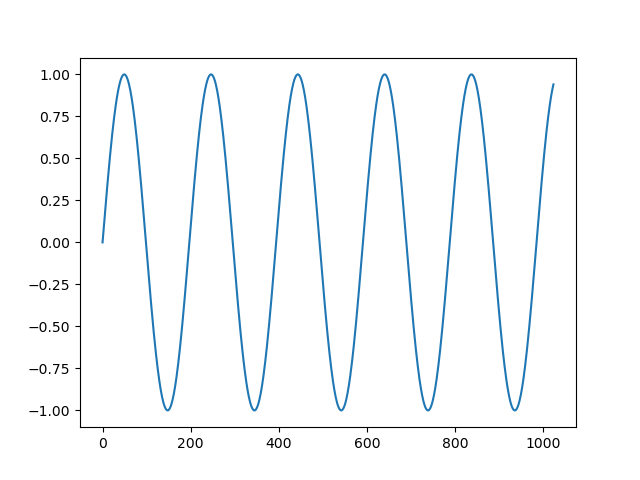
\includegraphics [scale=0.5] {signal.png}
	\caption{Сигнал c частотой $5.2$.}
	\label{img:signal}
\end{figure}
На рисунке 	\ref{img:spectrum} представлен спектр сигнала, полученный по формуле \textbf{?}:
\begin{figure}[ht]
	\centering
	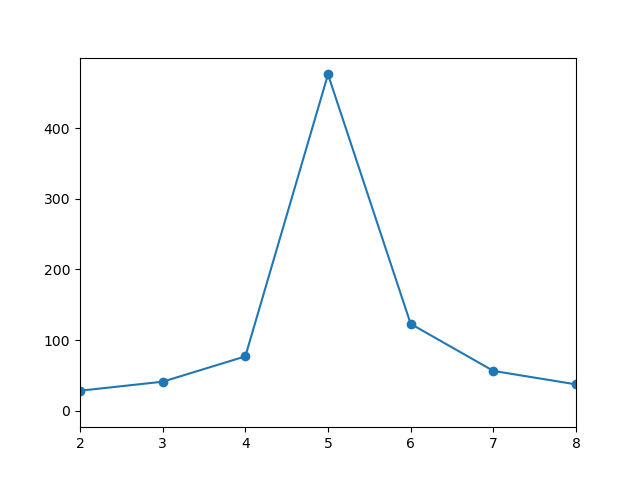
\includegraphics [scale=0.5] {spectrum.png}
	\caption{Спектр сигнала.}
	\label{img:spectrum}
\end{figure}
На рисунке \ref{img:interpolated_signal} представлен экстраполированный сигнал с добавленными нулевыми отчетами:
\begin{figure}[ht]
	\centering
	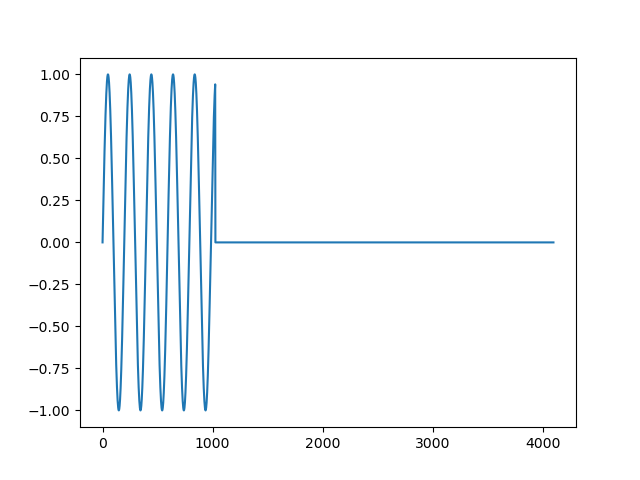
\includegraphics [scale=0.5] {interpolated_signal.png}
	\caption{Экстраполированный сигнал.}
	\label{img:interpolated_signal}
\end{figure}
Спектр экстраполированного сигнала с боковыми лепестками представлен на рисунке \ref{img:spectrum_of_interpolated_signal}, полученный по формуле \ref{eq:equation22}. Дискретный спектр расширяется, так как увеличивается время измерений из-за нулевых отчетов. Поэтому мы получаем более точную выборку спектра сигнала, так как количество точек в частотной области увеличилось. Полученный спектр имеет другой максимум гармоники сигнала. 
\begin{figure}[ht]
	\centering
	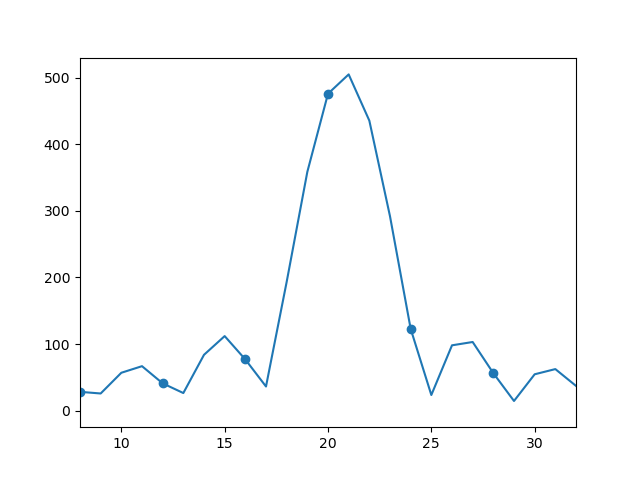
\includegraphics [scale=0.5] {spectrum_of_interpolated_signal.png}
	\caption{Спектр экстраполированного сигнала.}
	\label{img:spectrum_of_interpolated_signal}
\end{figure}

Применяя двойное интерполирование сигнала c параметром $k_{i1}=4$ (рисунок \ref{img:interpolated_signal}), получим спектр сигнала с двойной интерполяцией ($k_{i2}=4$):
\begin{figure}[ht]
	\centering
	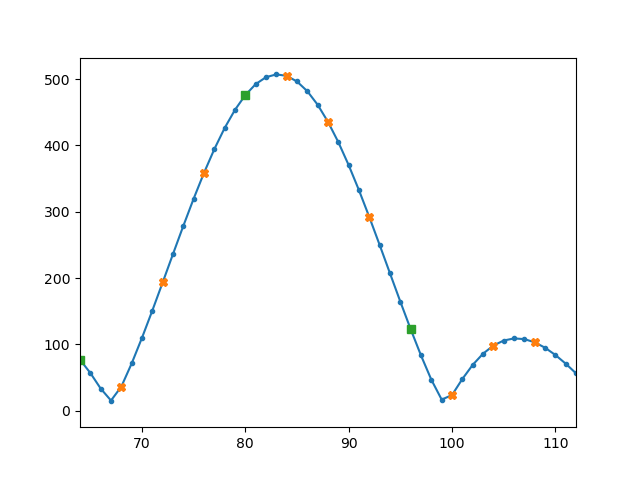
\includegraphics [scale=0.5] {spectrum_double_interpolated.png}
	\caption{Спектр с двойной интерполяцией сигнала ($k_{i2}=4$).}
	\label{img:spectrum_double_interpolated}
\end{figure}

\section{Разряженное Быстрое Преобразование Фурье} \label{sec:ch3/sect6} 
Spare FFT (SFFT, разряженное БПФ) -- алгоритм оценки спектра сигнала, содержащего малое число гармоник. В отличие от усеченного БПФ, которое находит небольшое число гармоник с заранее известным номером, SFFT находит гармоники, которые имеют более высокую амплитуду по сравнению с другими гармониками. Еще более существенное отличие SFFT от остальных БПФ заключается в том, что этот алгоритм является вероятностным и работает только для сигналов, для которых выполняются определенные условия (отсутствие в спектре большое числа гармоник с большой амплитудой, низкий уровень шума и другие).

SFFT является относительно новым подходом к вычислению спектра.
Первые публикации с идеями, лежащими в основе этого подхода, появились в
середине 90-х годов XX века \cite{kushilevitz1993learning}, после чего начали интенсивно появляться
новые алгоритмы для реализации этих идей \cite{hassanieh2012faster, hassanieh2012nearly, pawar2013computing, schumacher2014high, hassanieh2012simple}.
% Kushilevitz E., Mansour Y. Learning decision trees using the Fourier spectrum //SIAM Journal on Computing. – 1993. – Т. 22. – №. 6. – С. 1331-1348.
% Hassanieh H. et al. Faster GPS via the sparse Fourier transform //Proceedings of the 18th annual international conference on Mobile computing and networking. – 2012. – С. 353-364.
% Hassanieh H. et al. Nearly optimal sparse Fourier transform //Proceedings of the forty-fourth annual ACM symposium on Theory of computing. – 2012. – С. 563-578.
% Pawar S., Ramchandran K. Computing a k-sparse n-length discrete fourier transform using at most 4k samples and o (k log k) complexity //2013 IEEE International Symposium on Information Theory. – IEEE, 2013. – С. 464-468.
% Schumacher J., Püschel M. High-performance sparse fast Fourier transforms //2014 IEEE Workshop on Signal Processing Systems (SiPS). – IEEE, 2014. – С. 1-6.
% Hassanieh H. et al. Simple and practical algorithm for sparse Fourier transform //Proceedings of the twenty-third annual ACM-SIAM symposium on Discrete Algorithms. – Society for Industrial and Applied Mathematics, 2012. – С. 1183-1194.

Основное достоинство SFFT заключается в скорости его работы при большом числе входных данных. Он может успешно применяться для анализа сигналов в таких областях, как машинное обучение, GPS трекинг, компьютерная томография и другие.


Несмотря на обилие алгоритмов SFFT, общие принципы их работы похожи. Все алгоритмы выполняют оценку гармоник в два этапа:

\begin{itemize}
	\item выполняется процедура, традиционно называемая HashToBins, которая хэширует сигнал в несколько корзин (bin) (подробнее поясним ниже);
	\item выполняется процедура оценки частот.
\end{itemize}

При хэшировании сигналов в несколько корзин выполняются следующие действия:
% Что такое хэширование?
\begin{itemize}
	\item отчеты входного сигнала случайным образом распределяются между $B$ корзинами;
	\item отчеты, относящиеся к одной корзине, умножаются на некоторую
	оконную функцию (фильтр);
	\item внутри каждой корзины отчеты объединяются в группы, внутри группы отчеты суммируются;
	\item выполняется B БПФ над полученными в каждой корзине суммами.
	
	Количество корзин, оконная функция и размеры групп внутри корзин определяются в разных алгоритмах по-разному. Функция HashToBins может выполняться повторно с уточненными параметрами после второго этапа работы SFFT.
\end{itemize}

Процедура оценки частот сильно отличается от алгоритма к алгоритму, но обычно в ней присутствуют два этапа: оценка возможных позиций расположения гармоник и расчет значений этих гармоник.

Наибольших успехов в получение алгоритмов с низкой оценкой сложности достигла исследовательская группа из Массачусетского технологического института \cite{bottazzi2018new}. 
% Bottazzi G., Italiano G. F., Rutigliano G. G. A New Scalable Botnet Detection Method in the Frequency Domain //Cyber Criminology. – Springer, Cham, 2018. – С. 141-166.
Сложность предложенных ими алгоритмов составляет $O(K \log_{2} N)$ для расчета K гармоник сигнала по N входным отсчетами (если входной сигнал содержит не более K гармоник) и $O(K log_{2} N log_{2} \frac{N}{K})$ в общем случае \cite{indyk2014sparse, indyk2014nearly}.
% Indyk P., Kapralov M. Sparse Fourier Transform in Any Constant Dimension with Nearly-Optimal Sample Complexity in Sublinear Time. – 2014.
% Indyk P., Kapralov M., Price E. (Nearly) sample-optimal sparse Fourier transform //Proceedings of the Twenty-Fifth Annual ACM-SIAM Symposium on Discrete Algorithms. – Society for Industrial and Applied Mathematics, 2014. – С. 480-499.

Быстрые реализации SFFT для современных процессоров с набором SIMD инструкций были получены с помощью автоматического генератора кода проекта SPIRAL \cite{schumacher2014high, spiral}.
% Schumacher J., Püschel M. High-performance sparse fast Fourier transforms //2014 IEEE Workshop on Signal Processing Systems (SiPS). – IEEE, 2014. – С. 1-6.


На рисунке \ref{img:picture39} приведены
экспериментальные результаты оценки производительности SFFT по сравнению с классическим БПФ.
На нем по вертикальной оси отложено время выполнения FFT - $N^{22}$,
по горизонтальной — количество ненулевых частот K. Вертикальные линии
показывают время выполнения БПФ с помощью одной из наиболее оптимизированных
библиотек для классического БПФ. Верхняя линия — время работы алгоритма SFFT для случая, когда в сигнале заведомо присутствует не более $K$ гармоник, нижняя линия — в общем случае.

\begin{figure}[ht]
	\centering
	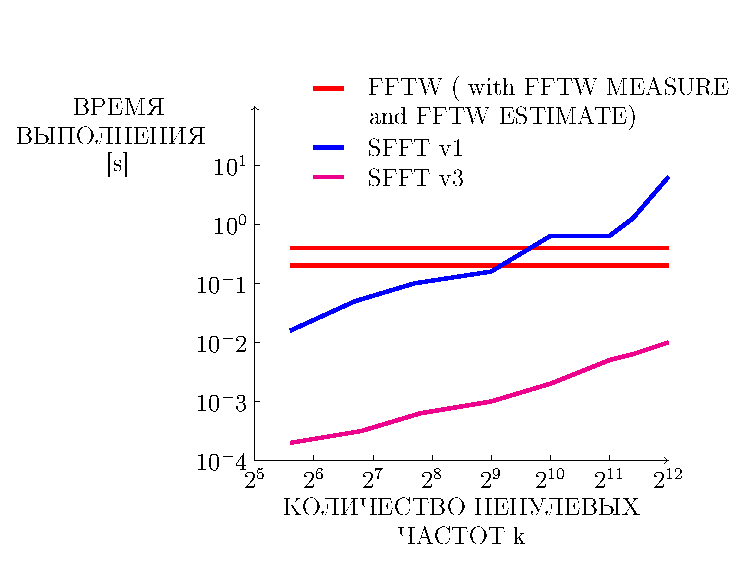
\includegraphics [scale=1.3] {Sparse Fourier Transform.pdf}
	\caption{Производительность разреженного преобразования Фурье.}
	\label{img:picture39}
\end{figure}

Как видно из графика, выигрыш в производительности разреженного преобразования Фурье при большом числе точек во входном сигнале и
малом числе гармоник может быть в несколько тысяч раз.

%%%%%%%%%%%%%%%%
Разряженное быстрое преобразование Фурье (SFFT, Sparse Fast Fourier Transform) -- алгоритм разработанный Хайтамом Хассани (Haitham Hassanieh) и другими \cite{hassanieh2012simple} для вычисления сигналов с разреженной частотной областью. Алгоритм улучшает асимптотическое время по сравнению с другими алгоритмами \cite{hassanieh2012nearly}.

Реализация SFFT на сайте http://groups.csail.mit.edu/netmit/sFFT/
доказывает, что алгоритм быстрее, чем FFT. Однако реализация SFFT не оптимизирована для современных аппаратных функций(иерархия кэша, многопоточность, наборы векторных инструкций).

На графике показано сравнение эталонной реализации SFFT и оптимизированной оптимизации SFFT и FFTW. Производительность SFFT была увеличена за счет различных оптимизаций. И теперь она так же эффективна, как высокопроизводительная библиотека FFTW для больших размеров ввода.

Библиотеку SFFT используют, если необходимо вычислисть дискретное преобразование Фурье сигнала и в сигнале используют несколько частотных компонентов. Существуют три версии SFFT. Третья версия SFFT не обрабатывает сигналы с шумом.

Первая и вторая версия SFFT могут применяться к зашумленным сигналам, но они работают только с определенными комбинациями входных параметров. Допустимые комбинации входных параметров представленные в таблице:
%  http://www.spiral.net/software/sfft/doc/usage.html#computing-sparse-dfts
\begin{table}[ht]
	\caption{Допустимые комбинации входных параметров}%
	\label{tbl:test3_1}%
	\fontsize{14pt}{14pt}\selectfont
	\begin{longtable*}[c]{|c|c|} 
		\hline
		Размер сигнала & Разреженность \\
		\hline
		$8192$ & $50$ \\
		$16384$ & $50$ \\
		$32768$	& $50$ \\
		$65536$	& $50$ \\
		$131072$ & $50$ \\
		$262144$ & $50$ \\
		$524288$ & $50$ \\
		$1048576$ & $50$ \\
		$2097152$ & $50$ \\
		$4194304$ & $50$ \\
		$8388608$ &	$50$ \\
		$16777216$ & $50$ \\
		$4194304$ & $50$ \\
		$4194304$ & $100$ \\
		$4194304$ & $200$ \\
		$4194304$ & $500$ \\
		$4194304$ & $1000$ \\
		$4194304$ & $2000$ \\ 
		$4194304$ & $2500$ \\
		$4194304$ & $4000$ \\
		\hline
	\end{longtable*}
\end{table}

Реализация SFFT находится в экспериментальном состоянии, библиотека не предназначена в качестве замены БПФ. Библиотеку SFFT следует использовать, если необходимо вычислить ДПФ сигнала. В сигнале должно присутствовать  несколько частотных компонентов. Библиотека SFFT оптимизирована для работы на современных процессорах $x86$ c поддержкой SSE.

%\cite{popovici2018large}
%Popovici D. T., Low T. M., Franchetti F. Large bandwidth-efficient FFTs on multicore and multi-socket systems //2018 IEEE International Parallel and Distributed Processing Symposium (IPDPS). – IEEE, 2018. – С. 379-388.

% http://www.spiral.net/software/sfft/doc/index.html
% http://groups.csail.mit.edu/netmit/sFFT/
% http://spiral.net/codegenerator.html

% Васеева Т. В., Альтман Е. А., Елизаров Д. А. Информационно-измерительная система для анализа гармоник сигнала в электрической сети //САПР и моделирование в современной электронике. – 2018. – С. 131-135.
% DOI: 10.30987/conferencearticle_5c19e5fbf19926.94126870

%Публикация в эту тематику
% R. G. McKilliam, I. V. L. Clarkson and B. G. Quinn, "Fast Sparse Period Estimation," in IEEE Signal Processing Letters, vol. 22, no. 1, pp. 62-66, Jan. 2015, doi: 10.1109/LSP.2014.2345737.

\section{Метод Якобсена} \label{sec:ch3/sect7}
Метод Якобсена основан на определении максимума спектра на основании трех точек БПФ \cite{4205098, ericjacobsen_cite, jacobsen1994local, jacobsen2007fast}. В качестве интерполируемой функции выступает квадратичная функция, графиком которой является парабола, близкая к спектру функции исследуемого напряжения (вершина параболы и максимальное значение спектра делят графики пополам). 
Пусть для квадратичной функции $u$ с максимальным коэффициентом функции $u(f_k)$  и истинным коэффициентом, достигнутым в максимуме $u(f_k + \delta)$. Тогда можно описать значение функции   в выбранных точках $f_{k-1}, f_k , f_{k+1}$ следующим образом:
\begin{equation}
\label{eq:equation2.7.1}
u(f_{k-1}) = a \cdot (f_{k-1}-\delta)^2+b
\end{equation}	
\begin{equation}
\label{eq:equation2.7.2}
u(f_k) = a \cdot (f_k-\delta)^2+b
\end{equation}	
\begin{equation}
\label{eq:equation2.7.3}
u(f_{k+1}) = a \cdot (f_{k+1}-\delta)^2+b,
\end{equation}	
Установив параметр $k$ в \ref{eq:equation2.7.1} равным $0$, получим следующее выражение для $\delta$:
\begin{equation}
	\label{eq:equation2.7.4}
	\bigtriangleup f = \frac{(|X_{k+1}|-|X_{k-1}|)}{(4|X_{k}|-2|X_{k-1}|-2|X_{k+1}|)}
\end{equation}

Далее проведем простую адаптацию формулы \ref{eq:equation2.7.4} для возможности оценки частоты комплексных значений БПФ \cite{ericjacobsen_cite}:

\begin{equation}
\label{eq:equation2.7.5}
\bigtriangleup f = \mathrm{Re}(\dfrac{(u(k+1)-u(k-1))}{2 \cdot u(k)-u(k+1)-u(k-1)})
\end{equation}

Параметр $\bigtriangleup f$  определяет отклонение порядкового номера максимальной частоты, найденный с использованием БПФ, от порядкового номера истинной максимальной частоты гармоник напряжения. Для всех интерполяционных методов порядковый номер истинной максимальной частоты и частота гармоник напряжения определяются по следующим формулам:
\begin{equation}
	\label{eq:equation2.7.6}
	f_{peak} = f_k + \bigtriangleup f
\end{equation}
\begin{equation}
	\label{eq:equation2.7.7}
	f_{tone} = f_{peak} \cdot \frac{f_s}{N}
\end{equation}

\begin{figure}[ht]
	\centering
	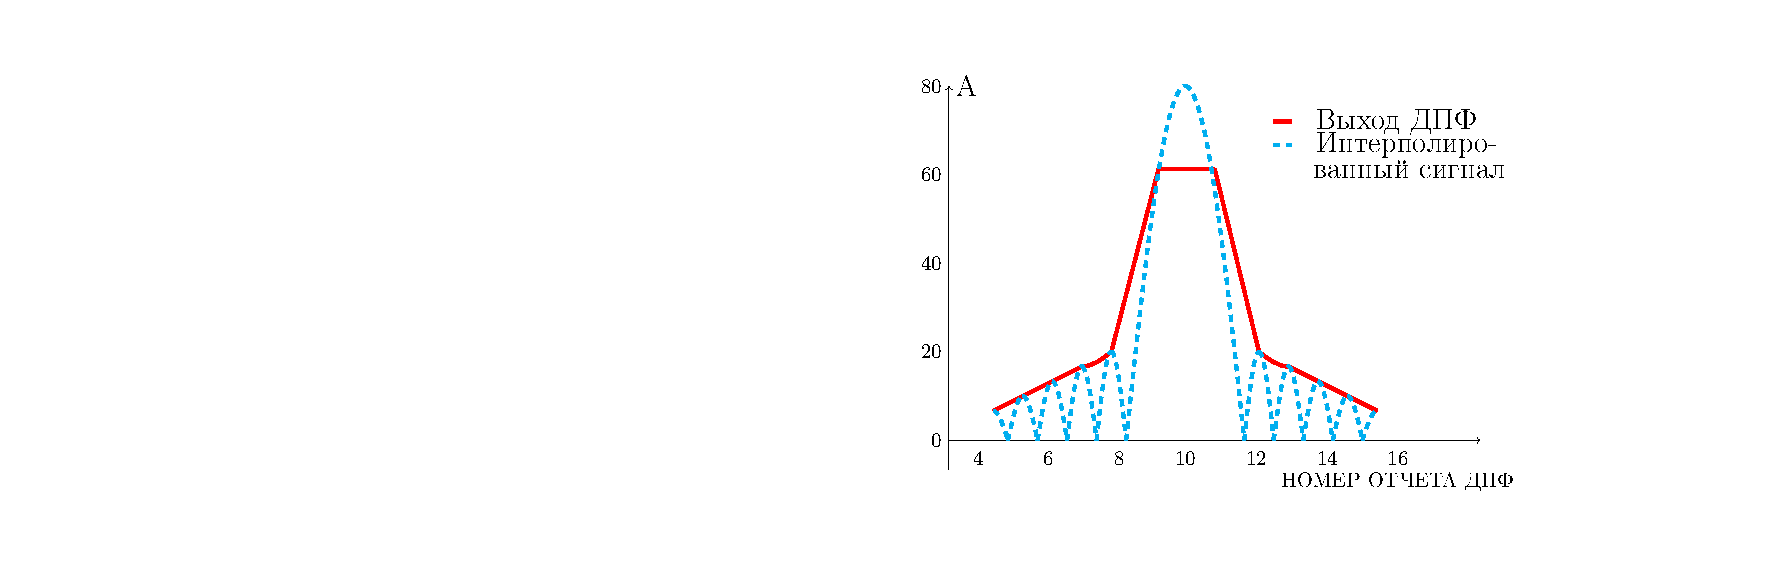
\includegraphics [scale=1] {Jacobsen's_method.pdf}
	\caption{Интерполяция пиков.}
	\label{img:picture3.7.2}
\end{figure}

\section{Метод чисел Фибоначчи} \label{sec:ch3/sect8}
Для определения коэффициента корреляции методом корреляционных функций необходимо перебрать все наборы эталонов. Тем самым, чтобы уменьшить вычислительную сложность метода, требуется сократить операцию перебора. Для этого были использованы методы определения максимума функции по заданным точкам \cite{Maximov1982Algorithms}. 
% Максимов Ю. А., Филлиповская Е. А. Алгоритмы решения задач нелинейного программирования //М.: МИФИ. – 1982. – Т. 52.

Один из методов оптимизации является метод чисел Фибоначи. Данный метод является одним из наиболее эффективных методов поиска экстремума. Метод требует двух вычислений функции на первой итерации, а на каждой последующей только по одному. 

Метод для определения максимума корреляционных функций выбран метод чисел Фибоначчи.
%Согласно чему?

Метод чисел Фибоначчи основан на последовательности чисел Фибоначчи, которая определяется следующим образом \cite{Matthews2001numerical}:
% Мэтьюз Д. Г. Численные методы. Использование MATLAB.–3-е издание./ДГ Мэтьюз, КД Финк //М., СПб.: Вильямс. – 2001. – Т. 716.
\begin{equation}
\label{eq:equation3.7.1}
F_{v+1} = F_v + F_{v-1}, v = 1, 2, 3, \cdots , F_0 = F_1 = 1
\end{equation} 

Последовательность Фибоначчи имеет вид: 

$0, 1, 1, 2, 3, 5, 8, 13, 21, 34, 55, 89, 144, 233, 377, 610, 987, 1597, 2584, 4181, 6765,$ 

$10946,\cdots,$ каждое последующее число равно сумме двух предыдущих чисел.

Пусть, что на  $k$-й итерации интервал неопределенности равен $[a_k, b_k]$. Рассмотрим две точки $\lambda_k$ и $\mu$ определяемые следующим образом:

\begin{equation}
\label{eq:equation3.7.2}
\lambda_k = a_k + \frac{F_{n-k-1}}{F_{n-k+1}} \cdot (b_k - a_k), k=1,2,\cdots, n-1
\end{equation} 

где $n$ – заданное общее число вычислений функции.

\begin{equation}
\label{eq:equation3.7.3}
\mu_k = a_k + \frac{F_{n-k}}{F_{n-k+1}} \cdot (b_k - a_k), k = 1,2,...n-1.	
\end{equation} 

Новый интервал неопределенности $[a_{k+1},b_{k+1}]$ будет равен $\lambda_k, b_k$, если $f(\lambda_k) > f(\mu_k)$ и $[a_k, \mu_k]$, если $f(\lambda_k) \leq f(\mu_k)$. В первом случае, учитывая \ref{eq:equation3.7.2} и полагая $v = n-k$ в \ref{eq:equation3.7.1}, получим:

\begin{equation}
\label{eq:equation3.7.4}
b_{k+1} - a_{k+1} = b_k - \lambda_k = b_k - a_k - \frac{F_{n-k-1}}{F_{n-k+1}} \cdot (b_k - a_k) = \frac{F_{n-k}}{F_{n-k+1}} \cdot (b_k - a_k)
\end{equation} 

Во втором случае, учитывая \ref{eq:equation3.7.3}, получаем:

\begin{equation}
\label{eq:equation3.7.5}
b_{k+1} - a_{k+1} = \mu_k - a_k = \frac{F_{n-k}}{F_{n-k+1}} \cdot (b_k - a_k)
\end{equation} 

Таким образом, в обоих случаях длина интервала неопределенности сжимается с коэффициентом $\frac{F_{n-k}}{F_{n-k+1}}$ .

На предварительном этапе алгоритма необходимо выбрать начальные границы отрезка $[a_1, b_1]$ и число итераций $n$ (коэффициент сокращения исходного интервала), рассчитать начальные точки деления ($\lambda_k$ и $\mu_k$) и значения в них целевой функции ($y_1 = f (\lambda_k)$  и $y_2 = f (\mu_k)$). На каждом шаге число $n$ уменьшается на единицу. На основном этапе алгоритма производится сравнение значений целевой функции в точках. Если $y_1 < y_2$ , то:

\begin{equation}
	\label{eq:equation3.7.6}
a = \lambda_k,
\lambda_k = \mu_k, \mu_k = b- (\lambda_k - a) 
\end{equation}

иначе:
\begin{equation}
\label{eq:equation3.7.7}
	b = \mu_k,
	\mu_k = \lambda_k, \lambda_k = a + (b - \mu_k) 
\end{equation}

После каждого шага проверяется условие: если $n=1$, то $x = \lambda_k = \mu_k$, в другом случае, алгоритм возвращает на основной этап.
 
%Листинг программы, реализующий метод, показан в приложении \textbf{?}

На рисунке \ref{img:picture3.7.1} представлена граф-схема метода Фибоначчи: 
\begin{figure}[ht]
	\centering
	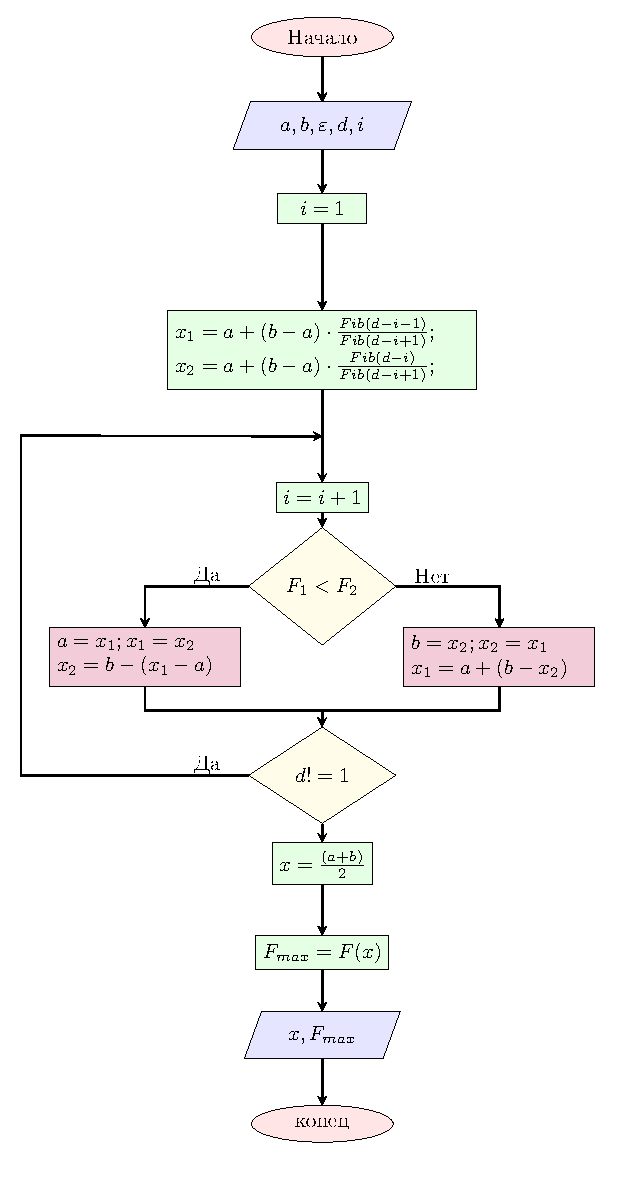
\includegraphics [scale=0.8] {GSA_Fibonacci_method}
	\caption{ГСА метода Фибоначчи.}
	\label{img:picture3.7.1}
\end{figure}

\section{Модернизация метода корреляционных функций} \label{sec:ch3/sect9}
Рассмотрим вывод формулы коэффициента корреляции между множеством $U$ и эталоном  $W_{ji}$. Из условия равенства двух комплексных чисел, в формуле \ref{eq:equation3.8}, амплитуды должны быть равны. Если в качестве окна выбирается симметричная функция, то функция $W(\omega)$ и множество ее значений $W_{ji}$ будут действительными. 
Когда эталоны $W_{ji}$ формируются достаточно часто, корреляционная функция $R(\bigtriangleup r - \bigtriangleup r_j)$ определяется как сумма квадратов значений $W_{ji}$ (обозначим эту сумму как $E$). Таким образом, формулу 	\ref{eq:equation3.10} для определения модуля амплитуды $v$-й гармоники можно переписать следующим образом:
\begin{equation}
	\label{eq:equation3.8.1}
	A_{\nu} = \frac{1}{E} \cdot \sqrt{\left({\displaystyle\sum_{i=1}^{i=M}\mathrm{Re}(U_i) \cdot W_{ji}} \right)^2 + \left({\displaystyle\sum_{i=1}^{i=M}\mathrm{Im}(U_i) \cdot W_{ji}} \right)^2}
\end{equation}

Для метода корреляционных функций необходимым условием при формировании наборов эталонов является использование эталонов с действительным спектром. Для оценки гармонических составляющих напряжения, необходимо разработать алгоритм получения эталонов с действительным спектром.

В качестве исследуемого напряжения рассмотрим следующую модель:
\begin{equation}
	\label{eq:equation3.8.2}
u'{t} = \displaystyle\sum_{v=0}^{v=N} A_v \sin \left({\frac{2 \cdot \pi}{T_s} \cdot v \cdot t + \varphi_v}\right) 
\end{equation}
где $A_v$ -- амплитуда $v$-й гармоники;

$\varphi_v$ – фаза $v$-й гармоники. 

Для ограничения длительности этого сигнала $u'(t)$ необходимо наложить на него весовую функцию $w(t)$, имеющую отличное от нуля значение на временном отрезке $ \left[ {-\frac{T_w}{2}, \frac{T_w}{2}} \right] $, со спектром $W(\omega)$. Таким образом, в результате наложения окна на сигнал получается новый, ограниченный во времени, сигнал $u(t)$:

\begin{equation}
	\label{eq:equation3.8.3}
	u(t) = u'{t} \cdot w(t) = \displaystyle\sum_{v=0}^{v=N} A_v e^{j \cdot \varphi_v} w(t) \cdot e^{j \cdot \frac{2 \cdot \pi}{T_s} \cdot  v \cdot t} 
\end{equation}

Эталонные сигналы формируются из синусоид с помощью наложения на них оконных функций. Как известно из свойств ДПФ, для того чтобы спектр заданного $N$ отсчетами сигнала был действительным, сигнал должен быть симметричен относительно точки $\frac{N}{2}$ \cite{sergienko2011digital}. Для получения симметричного эталона необходимо сделать симметричной синусоиду \cite{Altman2012formation}.
% Альтман Е. А., Елизаров Д. А. Формирование эталонной функции с действительным спектром для оценки спектра сигнала электрической сети //Динамика систем, механизмов и машин. – 2012. – №. 1.

Как показано на рисунке \ref{img:picture3.8.1}, для того чтобы синусоида была симметрична относительно точки $\frac{N}{2}$, необходимо подобрать ее фазу таким образом, чтобы значения в точках $\frac{N}{2} - 1$ и $\frac{N}{2} + 1$ были равны по модулю, но противоположны по значению  \cite{Altman2012formation}.

\begin{figure}[ht]
	\centering
	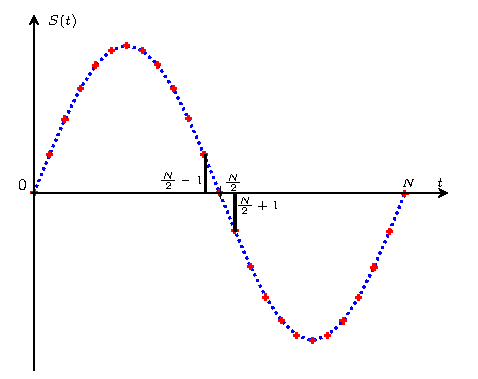
\includegraphics [scale=1.5] {Balanced_signal_representation}
	\caption{Представление симметричного сигнала.}
	\label{img:picture3.8.1}
\end{figure}

Выражения для определения фазы эталона  имеют вид:
\begin{equation}
\label{eq:equation3.8.4}
\sin \left[{\frac{2 \pi}{N}f \left( \frac{N+1}{2} \right) + phz(\delta)  } \right] = - \sin \left[{\frac{2 \pi}{N}f \left( \frac{N-1}{2}\right) + phz(\delta)} \right] 	 
\end{equation}

Так как синус нечетная функция, то формула \ref{eq:equation3.8.4} преобразуется к виду:
\begin{equation}
	\label{eq:equation3.8.5}
\sin \left[{\frac{2 \pi}{N}f \left( \frac{N+1}{2} \right) + phz(\delta)} \right] =  \sin \left[ - {\frac{2 \pi}{N}f \left( \frac{N-1}{2}\right) - phz(\delta)  } \right] 	 
\end{equation}

Аргументы синусов в формуле \ref{eq:equation3.8.5} равны с точностью до периода:
\begin{equation}
	\label{eq:equation3.8.6}
	 {\frac{2 \pi}{N}f \left( \frac{N+1}{2} \right) + phz(\delta)  }  =   - {\frac{2 \pi}{N}f \left( \frac{N-1}{2}\right) - phz(\delta)} + 2 \pi k  	 
\end{equation}

Выражение \ref{eq:equation3.8.6} относительно фазы выглядит следующим образом:
\begin{equation}
\label{eq:equation3.8.7}
2 \cdot phz (\delta) = \frac{2 \pi}{2 N}f \left(\frac{N - 1}{2} + \frac{N + 1}{2} \right)  
\end{equation}

После сокращений в \ref{eq:equation3.8.7} формула для нахождения фазы эталона примет вид:

\begin{equation}
	\label{eq:equation3.8.8}
	 phz (\delta) = \pi \cdot f + \pi \cdot k  
\end{equation}

Из условия равенства двух комплексных чисел, в формуле \ref{eq:equation3.8} значения угла $\varphi$ правой и левой части равны, с точностью до периода. Таким образом, фаза  $v$-й гармоники напряжения без учета функции $R(\bigtriangleup r - \bigtriangleup r_j)$  будет равна \cite{Altman2012definition}:
% Альтман Е. А., Елизаров Д. А. Определение фазы однотонального сигнала методом корреляционных функций //Инновационные проекты и новые технологии в образовании, промышленности и на транспорте. – 2012. – С. 323-326.
\begin{equation}
\label{eq:equation3.8.9}
\varphi_{v}'= \arctan \left({\frac{\displaystyle\sum_{i=1}^{i=M} \mathrm{Im}(U_i) \cdot W_{ji}}{\displaystyle\sum_{i=1}^{i=M} \mathrm{Re}(U_i) \cdot W_{ji}}
}\right) 
\end{equation}

Формула \ref{eq:equation3.8.9} позволяет определить фазу  $v$-й гармоники напряжения относительно эталона. Для получения фазы  $v$-й гармоники нужно учесть фазу эталона, а именно сдвиг фазы, связанный с отклонением значения параметра $\delta$ от базовой точки $В$, который определяется значением угла у набора эталона, максимально соответствующего исследуемому напряжению. Угол набора эталона $phz$, который максимально соответствует исследуемому напряжению, определяется следующим образом:

\begin{equation}
	\label{eq:equation3.8.10}
phz(\delta) = \pi \cdot f + \pi \cdot k
\end{equation}

где $f$ – частота гармоники напряжения для отклонения, равного параметру $\delta$.

Фаза  $v$-й гармоники напряжения определяется по следующей формуле:
\begin{equation}
	\label{eq:equation3.8.11}
\varphi_v = \left({\varphi ' + phz(\delta)}\right) +2 \pi k
\end{equation}

Для быстрого метода корреляционных функций необходимо определить точность, с какой будет производиться вычисления. Для этого определяется шаг формирования набора эталонов $h$. Далее определяется базовую точку $B$, вокруг которой будут создаваться эталоны, как ближайшее целое значение частоты измеряемого напряжения. Наборы эталонов формируются аналогичным образом, как и для метода корреляционных функций, только число эталонов должно быть число Фибоначчи. 

Амплитуда  $v$-й гармоники измеряемого напряжения определяется по формуле \ref{eq:equation3.10}. Значение наибольшей амплитуды гармоники соответствует коэффициенту корреляции. Максимальное значение корреляционной функции определяется согласно алгоритму Фибоначчи. Для этого на первой итерации коэффициенты корреляции определяются в двух точках, на каждой следующей – только в одной. Наибольшее значение коэффициента корреляции показывает на пару эталон-сигнал и, соответственно, на величину отклонения   от базовой точки. Фаза гармоники определяется по формуле \ref{eq:equation3.8.9}.

На рисунке \ref{img:picture3.8.2} отражены графики смещения оценки основной частоты напряжения в зависимости от уровня шума для быстрого метода корреляционных функций и модернизированного метода корреляционных функций. 
\begin{figure}[ht]
	\centering
	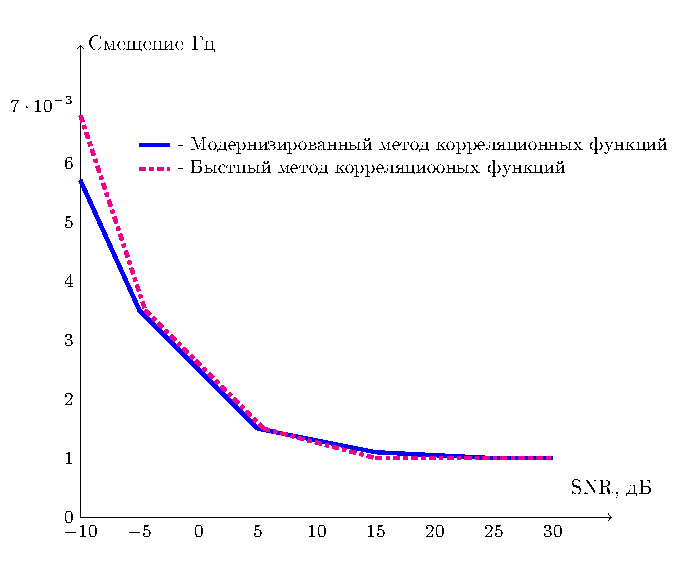
\includegraphics [scale=1] {voltage_fundamental_frequency_estimate_bias}
	\caption{Графики смещения оценки основной частоты напряжения в зависимости от уровня шума (быстрый метод корреляционных функций и модернизированный метод корреляционных функций).}
	\label{img:picture3.8.2}
\end{figure}

На рисунке \ref{img:picture3.8.3} отражена диаграмма, показывающая вычислительную сложность быстрого метода корреляционных функций и метода корреляционных функций. По оси абсцисс отложен шаг формирования набора эталонов $h$, по оси ординат – количество переборов наборов эталона.
\begin{figure}[ht]
	\centering
	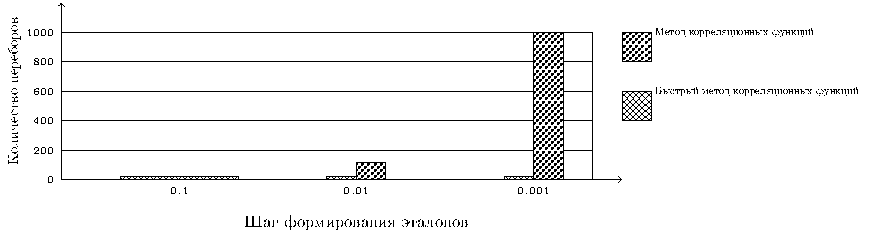
\includegraphics [scale=1.1] {Computational_complexity_diagram}
	\caption{Графики смещения оценки основной частоты напряжения в зависимости от уровня шума (быстрый метод корреляционных функций и модернизированный метод корреляционных функций).}
	\label{img:picture3.8.3}
\end{figure}

Вычислительная сложность быстрого метода корреляционных функций значительно ниже. Количество переборов быстрого метода корреляционных функций пропорционально натуральному логарифму от квадрата количества переборов метода корреляционных функций. Вычислительная сложность быстрого метода корреляционных функций равна $O(N+N\log(N))$, где $N$ – используемое число отсчетов БПФ.

\section{Прямой корреляционный метод с использованием быстрых алгоритмов обработки сигналов} \label{sec:ch3/sect10}
 Метод был исследован в среде разработке JetBrains PyCharm Community Edition 2018.3.1 x64 на языке программирования Python. 
 Изначально задаем входные параметры: частоту ($harmonics$), фазу ($phases$) и амплитуду ($amplitudes$), чтобы описать модель сигнала. На рисунке \ref{img:picture3.9.3} представлен зашумляем сигнал.
 \begin{figure}[ht]
 	\centering
 	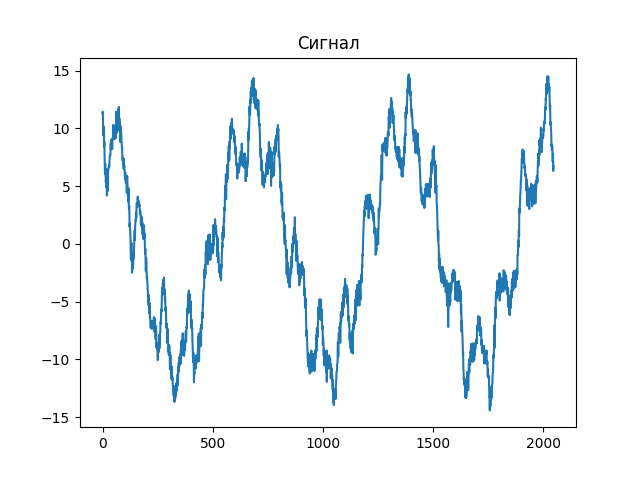
\includegraphics [scale=0.5] {Figure_1.png}
 	\caption{Сигнал.}
 	\label{img:picture3.9.3}
 \end{figure}
 Библиотека NumPy обеспечивает базовый функционал БПФ, расширяемый библиотекой SciPy. При этом обе библиотеки содержат функцию fft, основанную на динамической библиотеке FFTPACK языка Fortran.
 Функционал ДПФ библиотеки SciPy расположен в модуле scipy.fftpack.
 Далее ограничиваем сигнал оконной функцией Кайзера. Степень расширения Окна $kaiser_beta$ равна $14$, а ширина окна ($width_window$) равна 10. Создаем симетричное окно $window = kaiser(n+1, kaiser_beta)$, где $n=2048$. Далее применяем окно, чтобы уменьшить количество пиков. Исходная функция сигнала умножается на функцию окна $signal2 = signal * window[0:n]$. Добавляем нулевые значения, чтобы увеличить время измерения. Соответственно, спектр расширяется $spectrum3 = 2 * pi * fft(signal3) / n$, представлен на рисунке \ref{img:picture3.9.4}. Определим пик в интересующей области $sp = lambda x: abs(spectrum3[x])$. Далее находим предполагаемый пик и группы пиков. Определяем истинную вершину, фильтруя маленькие вершины. Листинг программы представлен в приложения \ref{app:Б}.

Граф-схема алгоритм поиска гармоник представленна на рисунке 	\ref{img:Diagram_GSA2}.
\begin{figure}[ht]
	\centering
	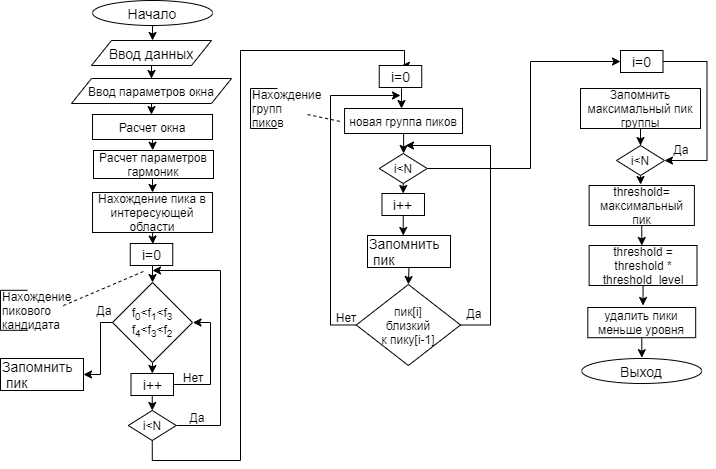
\includegraphics [scale=0.6] {Diagram_GSA2.png}
	\caption{ГСА алгоритма поиска гармоник.}
	\label{img:Diagram_GSA2}
\end{figure}

\begin{figure}[ht]
	\centering
	\includegraphics [scale=0.5] {Figure_2.png}
	\caption{Спектр расширенного сигнала.}
	\label{img:picture3.9.4}
\end{figure}

\section{Устройство для определения гармоник или спектра сигнала электрической сети} \label{sec:ch3/sect11}

Основным направлением в применении цифровой обработки сигналов является спектральный анализ. Каждый сигнал, который изменяется во времени, имеет частотный спектр. Электрические сигналы можно 
анализировать в частотной области с помощью анализаторов спектра, во временной области с помощью осциллографов. К анализатору спектра предъявляют различные требования измерений по максимальной частоте входного сигнала. Ряд Фурье представляет разложение несинусоидальной периодической функции на синусоидальные компоненты и позволяет рассматривать сигналы из временной области в частотной \cite{information-measuring2018}.

На практике сигнал подвергают анализу, дискретизации (взятие выборки), квантованию по амплитуде с помощью аналого-цифрового преобразователя (АЦП, AD Converter). Для выборки сигналов, прошедших 
через фильтр низких частот, где минимальная частота выборки определяется максимальной частотой сигнала (теорема В. А. Колельникова): 
\begin{equation}
 \label{eq:equation3.9.1}
 f_s \geqslant 2f_{input.max},
\end{equation}

где $f_s$ – частота выборок, Гц;

$f_{input.max}$ – максимальная частота сигнала, Гц.

Для преобразования Фурье используют лишь некоторую часть сигнала с ограниченным числом выборок 
$N$. Этот процесс называется «оконной выборкой».

Расчет спектра сигнала на основе выборок во временной области обычно называют дискретным преобразованием Фурье (ДПФ, Discrete Fourier Transform – DFT). Востребованность данного метода заключается в том, что сигнал легче обработать, когда он представлен в частотной области.
\begin{equation}
\label{eq:equation3.9.2}
	\underline{X}(k) = \sum^{N-1}_{n=0} \underline{x}(nT_s) \cdot e^{-j2 \pi kn/N},
\end{equation}

где $T_s$  – период выборок, с;

$\underline{X}(k)$ –  значение спектра в точке $kf_s/N$;

$k$ – номер частотного отчета ($k=0,1,2\ldots m$);

$N$ – длина DFT.

Число вычислительных операций зависит от используемого алгоритма. Быстрое преобразование Фурье (БПФ, FFT – Fast Fourier Transform) оптимизирует число операций. Анализаторы спектра, которые работают по данному алгоритму, называют БПФ-анализаторы. В его состав входят фильтр нижних частот (ФНЧ), АЦП, оперативное запоминающее устройство (ОЗУ, RAM – Random Access Memory), БПФ и дисплей (рисунке \ref{img:picture3.9.1}). 
\begin{figure}[ht]
	\centering
	\includegraphics [scale=0.7] {block_diagram_of_an_FFT_analyzer.png}
	\caption{Структурная схема БПФ-анализатора.}
	\label{img:picture3.9.1}
\end{figure}

Однако данный анализатор обладает низкой точностью измерения гармоник входного сигнала \cite{Rauscher2006basics}.
% 1. Раушер К., Йанссен Ф., Минихольд Р. Основы спектрального анализа //М.: Горячая линия-Телеком. – 2006.
При ограничении числа точек в цифровом сигнале образуются пробелы между отчетами в спектре сигнала.

Анализатор гармоник, или спектр сигнала электрической сети содержит: блок $\textnumero 1$ –  фильтр нижних частот $1$ (ФНЧ$1$, Low-pass filter), вход, которого соединен с анализатором, а выход соединен с с аналого-цифровым преобразователем (АЦП, AD Converter). Частота среза фильтр равна максимальной частоте сигнала $f_{sf} = f_{input.max} $. Вход управления АЦП соединен с блоком памяти $\textnumero 3$ – оперативным запоминающим устройствам (ОЗУ, RAM – Random Access Memory), а выход – с блоком $№4$ «Передискретизация» (Resampling). Значения выборки сохраняются в памяти после разбиения диапазона отчетных значений сигнала на конечное число уровней и округление этих значений (квантование – quantization). 

Вход управления «Передискретизации» соединен с блоком $\textnumero 5$ – фильтром нижних частот $2$ (ФНЧ$2$, Low-pass filter). А выход соединен с блоком $\textnumero 6$ – «SFFT» (Sparse Fast Fourier Transform). Выход соединен с дисплеем, блок $\textnumero 7$. Блок дисплея показывает частотный спектр сигнала.

Блок «Передискретизация» позволяет точнее определять значения 
частоты основной гармоники \cite{Thomasi2017electronic}. 
% 9. Томаси У. Электронные системы связи. – Litres, 2017.
Передискретизация – это операция, которая изменяет частоту дискредитации. При ограничении частоты 
дискретизации образуются пробелы в спектре сигнала, поэтому необходимо добавить нулевые отчеты в напряжение гармонических составляющих. При увеличении числа точек во временной области спектр сигнала не меняется в интересующийся нас области. Передискретизация приводит к тому, что БПФ не будет справляться из-за ограничения вычислительных ресурсов. Поэтому увеличение числа точек 
на современных устройствах служит причиной того, что алгоритм БПФ не выполняется. Следовательно, для нахождения спектра сигнала лучше использовать SFFT.

Блок «SFFT» – это алгоритм, разработанный H. Hassanieh, P. Indyk, D. Katabi, E. Price для вычисления дискретных преобразований Фурье по сигналам с разреженной частотной областью (число ненулевых гармоник). Алгоритм улучшает асимптотическое время по сравнению с предыдущими методами \cite{hassanieh2012nearly, gilbert2002near}. 
% 2. Hassanieh H. et al. Nearly optimal sparse Fourier transform //Proceedings of the forty-fourth annual ACM symposium on Theory of computing. – 2012. – С. 563-578.

% 8. Gilbert A. C. et al. Near-optimal sparse Fourier representations via sampling //Proceedings of the thiry-fourth annual ACM symposium on Theory of computing. – 2002. – С. 152-161.

При определенных условиях, алгоритм SFFT быстрее, чем современные библиотеки FFT (Fast Fourier Transform) в тысячи раз \cite {6986055, spiral}. 
% 10. J. Schumacher and M. Püschel, "High-performance sparse fast Fourier transforms," 2014 IEEE Workshop on Signal Processing Systems (SiPS), Belfast, UK, 2014, pp. 1-6, doi: 10.1109/SiPS.2014.6986055.

% 11. Spiral Home page. – URL: http://www.spiral.net/ (дата обращения 01.09.2018).

Асимптотическое время автономной работы SFFT не является линейным по размеру сигнала, как в БПФ. Время работы увеличивается медленнее: для SFFT – $N$, для БПФ – $NlogN$.
Структурная схема устройства для определения гармоник или спектра сигнала электрической сети представлена на рисунке.
\begin{figure}[ht]
	\centering
	\includegraphics [scale=1] {block_diagram_of_a_device_for_determining_harmonics_or_spectrum_of_an_electrical_network_signal.png}
	\caption{Структурная схема Анализатора SFFT и Resampling.}
	\label{img:picture3.9.2}
\end{figure}

\section{Выводы по разделу} \label{sec:ch3/sect12}
На основании анализа, произведенного в третьем разделе, были получены следующие результаты:

\begin{enumerate}
\item методы, основанные на интерполировании смежных гармоник, позволяют достичь высокой точности, во многих случаях достаточной для практического применения, однако они не позволяют достичь точности оптимальной несмещенной оценки;

\item можно выделить два подхода к построению алгоритмов на основе корреляционного анализа: использование итерационного процесса для нахождения частоты, амплитуды и фазы каждой гармоники и использование техники дополнения нулями сигнала с целью уплотнения гармоник в спектре сигнала. Оба метода требуют существенно больших вычислительных ресурсов, чем методы основанные на интерполировании, но обеспечивают оптимальную несмещенную оценку;

\item время расчета параметров гармоник многотонального сигнала с помощью техники дополнения нулями может быть существенно снижено за счет применения разряженного быстрого преобразования Фурье;

\item реализация итерационного оптимизационного метода нахождения гармоник на основе чисел Фиббоначи при небольшом числе обсчитываемых гармоник обеспечивает быстродействие, близкое к итерационным методам; 

\item реализация метода дополнение нулями сигнала при использовании разряженного преобразования Фурье имеет быстродействие менее чем на порядок худшее, чем итерационные методы, при этом быстродействие не зависит от числа обсчитываемых гармоник. Также нужно отметить больший объем памяти, требуемый для этого метода, который при этом не является критичным для современных вычислительных устройств.
\end{enumerate}
           % Глава 3
% ПЛАН
%# Глава 4 – Применение алгоритмов оценки параметров многотональных сигналов для анализа гармоник и интергармоник в электрических сетях на железнодорожном транспорте
%
%Выводы по главе:
%
%- В современных стандартах по анализу спектра в электрических сетях большее внимание уделяется нахождению интергармонических составляющих. Поскольку интергармонические составляющие имеют малую энергию по отношению к другим гармоникам и шуму, к алгоритмам для нахождения параметров гармоник возрастают требования по точности определения амплитуды в условиях высокого шума.
%- В стандартах также указывается требования о нахождение всех гармоник по 40 включительно, что, вместе с требованием о нахождении интеграмоник приводит к большому числу анализируемых гармонических составляющих сигнала.
%- Исходя из требований стандарта и анализа свойств изученных алгоритмов для анализа спектра сигнала в силовых электрических сетях железнодорожного транспорта рекомендуется использование метода дополнения сигнала нулями с применением разряженного преобразования Фурье.
%- Время расчета спектра реального сигнала этим методом на современном компьютере начального уровня составляет единицы секунд, что позволяет говорить о его приемлемом быстродействии для решения практических задач.

\chapter{Применение алгоритмов оценки параметров многотональных сигналов для анализа гармоник и интергармоник в электрических сетях на железнодорожном транспорте}\label{ch:ch4}

В четвертом разделе рассматривается понятие, характеризующее качества электрической энергии в электрических сетях систем электроснабжения переменного тока с частотами 50 и 60~Гц и порядок оценки результатов. Стандарты в области контроля определяющие состав показателей качества электрической энергии, методику измерений и характеристики средств измерений. В результате анализа производится сравнение государственных стандартов Российской Федерации (ГОСТ~Р) и международных стандартов (МЭК, IEC -- International Electrotechnical Commission), которые описывают требования и нормы КЭ \cite{IEC}.
%\hyperlink{https://www.iec.ch/}{[199]}. 
% [199 - International Electrotechnical Commission [Электронный ресурс] – Режим доступа:https://www.iec.ch/]

В четвертом разделе произведен сравнительный анализ существующих средств контроля учета показателей КЭ. В заключении описывается основные задачи и виды контроля КЭ.

В последние годы правительством Российской Федерации разрабатывались и принимались нормативные правовые документы, которые
определяют государственную важность обеспечения высокой
энергетической, экономической и экологической эффективности производства,
передачи, распределения и потребления электрической энергии. Основопологащие документы:
\begin{itemize}
	\item Энергетическая стратегия политики России определяет цели и задачи развития страны в период до 2030 года, утвержденная распоряжением Правительства Российской Федерации от 13 ноября 2009~г. N 1715-р \cite{energy_strategy}. 
	\item Федеральный закон от 26 июля 2019~г. №~261-ФЗ «Об энергосбережении и о повышении энергетической эффективности и о внесении изменений в отдельные законодательные акты Российской Федерации (с изменениями на 26 июля 2019~года)»\cite{energy_saving_law_2019}.
\end{itemize}


Темпы потребления электроэнергии зависят от географического расположения региона. Главным направлением перспективного развития энергетики в России является, повышение эффективности контроля качества электрической энергии (КЭ). 
Министерство энергетики Российской Федерации (Минэнерго России) является федеральным органом исполнительной власти по государственной политике и нормативно-правовому регулированию в области энергосбережения. Минэнерго России управляет государственным имуществом в сфере производства, а также использования топливно-энергетических ресурсов. Энергетическая политика России позволяет использовать природные энергетические ресурсы в соответствии с приоритетами развития страны для устойчивого роста экономики. 

Реализация настоящей стратегии, является повышение эффективности 
контроля качества электрической энергии (КЭ). Поэтому необходимо уделять большее внимание методам контроля и анализа показателей КЭ. 
Каждое электрооборудование предназначено для работы при определенных параметрах электрической энергии: номинальной частоте, напряжении, токе и других параметрах. Поэтому для нормальной работы необходимо обеспечить требуемое качество электрической (КЭ).  КЭ определяется совокупностью ее характеристик, при которых электрооборудование нормально функционирует. Несоответствие показателей КЭ или свойства электрической энергии, которые ухудшают КЭ и приводят к преждевременному износу электрооборудования. 

Существенный вклад в решение рассматриваемых проблем внесли отечественные ученые: В.Г.~Аввакумов, В.Д.~Бардушко, Г.Я.~Вагин, В.Э.~Воротницкий, Н.И.~Воропай, В.Н.~Горюнов, А.З.~Гамм, И.В.~Жежеленко, Ю.С.~Железко, В.Г.~Курбатский, В.З.~Манусов, И.С.~Рокотян, М.О.~Доливо-Добровольский, В.Т.~Черемисин, М.Г.~Шалимов, А.К.~Шидловский и другие. 

%% УЧЕНЫЕ:
%В.Г. Аввакумов (Аввакумов В. Г. Влияние несимметрии и несинусоидальности напряжения на работу силовых конденсаторов [Текст]: (Энергет. параметры конденсаторных установок систем энергоснабжения электр. ж. д.): Автореферат дис. на соискание учен. степени кандидата техн. наук / Омский ин-т инженеров ж.-д. транспорта.)
%В.Д. Бардушко (Бардушко, Валерий Данилович – доктор технических наук. Анализ и параметрический синтез систем тягового электроснабжения: диссертация ... доктора технических наук: 05.13.01. - Иркутск, 2001. - 264 с.) 
%Г.Я. Вагин (Вагин Геннадий Яковлевич (род. 10 марта 1938 г.) – доктор технических наук, профессор кафедры электроэнергетики и электроснабжения Нижегородского государственного технического университета. Заслуженный деятель науки РФ. Более 200 научных работ, в том числе 16 монографий и 16 учебных пособий.) 
%В.Э. Воротницкий (Воротницкий, Валерий Эдуардович – доктор технических наук. Методы и средства совершенствования управления распределительными электрическими сетями и повышения их экономичности: автореферат дис. ... доктора технических наук: 05.14.02 / НИИ электроэнергетики АО ВНИИЭ. - Москва, 1996. - 54 с.)
%Н.И. Воропай (Воропай, Николай Иванович – (род. 1 ноября 1943 года) – физик, член-корреспондент РАН, заслуженный деятель науки Российской Федерации, лауреат премии имени Г. М. Кржижановского, доктор технических наук)
%В.Н. Горюнов (Горюнов, Владимир Николаевич – доктор технических наук. Беспазовые электрические машины с многополюсными и униполярными индукторами на высококоэрцетивных магнитах: Теория, мат. моделирование, совершенствование конструкций: диссертация ... доктора технических наук: 05.09.01. - Омск, 1993. - 417 с.) 
%А.З. Гамм (Гамм, Александр Зельманович (9 октября 1938 года, Волгоград) – физик, лауреат премии имени Г. М. Кржижановского. Методы анализа режимов электроэнергетических систем по данным измерений: диссертация ... доктора технических наук : 05.14.02. - Иркутск, 1981. - 337 с.)
%И.В. Жежеленко (Игорь Владимирович Жежеленко (род. 1930) – украинский учёный в области электроснабжения промышленных предприятий, доктор технических наук, профессор, заведующий кафедрой «Электроснабжение промышленных предприятий» ПГТУ, ректор Ждановского металлургического института / Приазовского Государственного Технического университета (1981—2003).)
%Ю.С. Железко (Железко, Юрий Станиславович. Научно-методические основы стратегии снижения потерь и повышения качества электроэнергии в электрических сетях: автореферат дис. ... доктора технических наук: 05.14.02. - Москва, 1996. - 46 c.) 
%В.Г. Курбатский (Курбацкий, Виктор Григорьевич. Мониторинг качества электроэнергии в электрических сетях России для выбора мероприятий по обеспечению электромагнитной совместимости: автореферат дис. ... доктора технических наук: 05.14.02 / Сиб. отд-ние. Сиб. энергетический ин-т им. Л. А. Мелентьева. - Иркутск, 1997. - 42 с.)
%В.З. Манусов (Манусов, Вадим Зиновьевич. Нелинейные стохастические модели для анализа и планирования режимов электрических систем: диссертация ... доктора технических наук: 05.14.02. - Новосибирск, 1985. - 408 с.:) 
%И.С. Рокотян (Сергей Сергеевич Рокотян (1908, Умань – 1977) – советский инженер-энергетик, учёный.)
%М. О. Доливо-Добровольский (Михаил Осипович Доливо-Добровольский (21 декабря 1861 [2 января 1862], Гатчина – 15 ноября 1919, Гейдельберг) – известный российский электротехник, один из создателей техники трёхфазного переменного тока.)
%В.Т. Черемисин (Черемисин, Василий Титович. Совершенствование методов расчета режимов приема и потребления электрической энергии в условиях несимметрии и несинусоидальности электротяговой нагрузки переменного тока: диссертация ... доктора технических наук: 05.22.09. - Омск, 1996. - 444 с.)
%М.Г. Шалимов (Шалимов, Михаил Георгиевич. Сопротивления проводов, линий электропередачи и контактной сети в спектре повышенных частот [Текст]: (Теория и расчет): Автореферат дис. на соискание ученой степени доктора технических наук. (435) / Омский ин-т инженеров ж.-д. транспорта. - Омск: [б. и.], 1970. - 34 с.)
%А.К. Шидловский (Анатолий Корнеевич Шидловский (укр. Анатолій Корнійович Шидловський), (род. 10 октября 1933, с. Веприк (ныне Бобровицкого района Черниговской области Украина) — украинский и советский учëный в области электротехники и электроэнергетики, профессор, член-корреспондент АН УССР (с 1978), действительный член (академик) Национальной академии наук Украины. Вице-президент НАН Украины (1998—2004). Заслуженный деятель науки и техники Украины (1995). Лауреат Государственной премии УССР (1982))




\section{Понятие качества электрической энергии}\label{sec:ch4/sect1} 
ГОСТ Р~--~государственный стандарт Российской Федерации, используется только на территории России.

Повышение КЭ является основным фактором улучшения энергетической эффективности промышленных предприятий \cite{Energy_Saving2009}. 
% [10 - Закон Ф. Об энергосбережении и о повышении энергетической эффективности и о внесении изменений в отдельные законодательные акты Российской Федерации //№ 261-ФЗ от 23.11. – 2009.]
%http://www.consultant.ru/document/cons_doc_LAW_93978/

Понятие качества электрической энергии (КЭ) описано государственном стандарте (ГОСТ) 32144--2013~\cite{GOST32144-2013} п.~3.1.38, обозначает степень соответствия характеристик электрической энергии в данной точке электрической системы совокупности нормированных показателей КЭ.

Задача исследования -- улучшить показатели качества электрической энергии (ПКЭ) в электрических сетях систем электроснабжения, совершенствуя средства измерительных устройств для определения гармоник. При разработке технического устройства должны учитываться ПКЭ  согласно действующим нормативам. 

Введен целый ряд нормативных документов (МЭК, ГОСТ). Изменение стандартов в области измерений электрической энергии показано на рисунке~\ref{img:picture1} \cite{GOST30804.4.30-2013, GOST30804.4.7-2013, GOST32144-2013, GOST_R8.655-2009, GOSTR51317.4.15-2012, GOST33073-2014, GOST8.622-2013}. 

В работе рассмотрены методы контроля и анализа показателей качества электрической энергии, характеризующих несинусоидальность напряжения. Для анализа отклонения формы кривой от синусоиды напряжения разлагаются на спектральные составляющие. Таким образом, чтобы повысить точность измерения показателей несинусоидальности напряжения, необходимо уделить внимание повышению точности оценки спектральных составляющих напряжения. Для этого потребуется выполнить модернизацию существующих методов и необходимо создание нового алгоритма оценки гармонических и интергармонических составляющих напряжения. 


Наличие интергармоник и гармоник оказывает негативное влияние на оборудование. Из-за возникновения гармоник в электрических сетях происходит перегрев оборудования, поэтому уменьшается его срок службы. Интергармоники наблюдаются при увеличении количества нагрузок в дополнение к гармоникам. Наличие асинхронных включений частотно-регулируемых электроприводов, выполненных на основе полупроводниковых преобразователей является причиной появления интергармоник. Так же интергамоники возникают при изменении тока в оборудовании, которое приводит к колебаниям напряжения. 

В настоящее время на рынке средства измерений показателей качества электрической энергии представлено большое количество приборов российского и зарубежного производства. Зарубежные приборы удобны и надежны в эксплуатации, но они дороже отечественных аналогов.

\begin{figure}[ht]
	\centerfloat{
		\includegraphics[scale=0.8]{picture1}
	}
	\caption{Развитие государственных стандартов в области контроля КЭ.}\label{img:picture1}
\end{figure}
%Действующие стандарты на рисунке

% [179 - ГОСТ 30804.4.30-2013 (IEC 61000-4-30:2008) Электрическая энергия. Совместимость технических средств электромагнитная. Методы измерений показателей качества электрической энергии (с Поправкой) [Электронный ресурс] / Режим доступа: http://docs.cntd.ru/document/1200104665]

% [4 - ГОСТ 30804.4.7-2013 (IEC 61000-4-7:2009) Совместимость технических средств электромагнитная. Общее руководство по средствам измерений и измерениям гармоник и интергармоник для систем электроснабжения и подключаемых к ним технических средств (с Поправкой) [Электронный ресурс] / Режим доступа: http://docs.cntd.ru/document/1200103652]

% [125 - ГОСТ 32144-2013 Электрическая энергия. Совместимость технических средств электромагнитная. Нормы качества электрической энергии в системах электроснабжения общего назначения [Электронный ресурс] – Режим доступа: http://docs.cntd.ru/document/1200104301/]

% [136 - ГОСТ Р 8.655-2009 Государственная система обеспечения единства измерений (ГСИ). Средства измерений показателей качества электрической энергии. Общие технические требования (с Изменением N 1) [Электронный ресурс] / Режим доступа: http://docs.cntd.ru/document/1200075494/]

% [194 - ГОСТ Р 51317.4.15-2012 (МЭК 61000-4-15:2010) Совместимость технических средств электромагнитная. Фликерметр. Функциональные и конструктивные требования [Электронный ресурс] / Режим доступа: http://docs.cntd.ru/document/1200096463]

% [195 - ГОСТ 33073-2014 Электрическая энергия. Совместимость технических средств электромагнитная. Контроль и мониторинг качества электрической энергии в системах электроснабжения общего назначения (с Поправкой) [Электронный ресурс] / Режим доступа: http://docs.cntd.ru/document/1200115349]

% [196 - ГОСТ 8.622-2013 Государственная система обеспечения единства измерений (ГСИ). Испытательное оборудование для определения коэффициента проникания тест-аэрозоля через средства индивидуальной защиты органов дыхания. Методика аттестации [Электронный ресурс] / Режим доступа: http://docs.cntd.ru/document/1200108162]

Основополагающим нормативным документом в Российской Федерации, регламентирующим положения связанные с КЭ в Российской Федерации, был ГОСТ~13109--97 \cite{GOST13109-97}. 

Стандарт не отвечал современным реалиям и заменен на ГОСТ~32144--2013 \cite{GOST32144-2013}, действует с 01.07.2014~г. приказом Росстандарта. Российский стандарт соответствует европейскому ЕN 50160:2010 <<Характеристики напряжения электричества, поставляемого общественными распределительными сетями>> \cite{ЕN50160:2010}. Действующий зарубежный стандарт DIN~EN~50160--2011 \cite{DINEN50160-2011}. DIN (Deutsches Institut für Normung – немецкий институт по стандартизации) – государственный стандарт Германии. EN (EuroNorm) – европейский стандарт, принятый Европейским комитетом по стандартизации CEN (European Committee for Standardization).

% [11 - 11.	EN 50160:2010 Voltage characteristics of electricity supplied by public electricity networks [Электронный ресурс] / Режим доступа: https://infostore.saiglobal.com/preview/98699522296.pdf?sku=859794_saig_nsai_nsai_2045468]

Новый стандарт ГОСТ~32144--2013 по требованиям к КЭ учитывает рекомендации положений международных стандартов и новых национальных стандартов по методам и средствам измерения и оценки ПКЭ, а также сближает структуру и положения данного стандарта с европейским стандартом ЕN~50160:2010.
Определение понятия средства измерений (СИ) в ГОСТ~30804.4.7--2013 \cite{GOST30804.4.7-2013}.
СИ предназначенных для, измерений спектральных составляющих напряжения и тока в полосе частот до 9 кГц, которые наложены на основные составляющие в системах электроснабжения частотой 50 и 60 Гц.


Некоторые принципиальные отличия  ГОСТ~32144--2013 \cite{GOST32144-2013} от предыдущего стандарта ГОСТ~13109--97 \cite{GOST13109-97}: 
%\noindent Маркированный список:
\begin{itemize}
	\item Отличие по интервалам усреднения показателям качества электроэнергии (отклонение частоты -- 10~сек., вместо 20~сек. в ГОСТ~13109--97; не симметрия напряжения -- интервал усреднения 10~мин., вместо 3~сек. в ГОСТ~13109--97; гармонические составляющие напряжения -- 10~мин., вместо 3~сек. в ГОСТ~13109--97) с интервалом периода в одну неделю, вместо суток в ГОСТ~13109--97.
	\item Измерения согласно ГОСТ~30804.4.30--2013 (IEC~61000--4--30:2008) \cite{GOST30804.4.30-2013} и ГОСТ~30804.4.7–-2013 (IEC~61000--4--7:2009) \cite{GOST30804.4.7-2013}.
	\item Для медленных изменений напряжения исключены режимы наименьших и наибольших нагрузок.
	\item Добавлены таблицы классификации провалов напряжения по остаточному напряжению.
\end{itemize}

При невыполнении энергоснабжающей организации требований к ПКЭ (в соответствии с ГОСТ 32144-2013 \cite{GOST32144-2013}, обязательным к применению в соответствии с
частью 1 статьи 46 Федерального закона от 27.12.2002 № 184-ФЗ «О техническом регулировании») наступает административная ответственность по статье $14.43$
«Кодекса Российской Федерации об административных правонарушениях» \cite{Serkov2017Problems} %c. 53.

Кроме Российских стандартов, существуют Международные регламентирующие документы по мониторингу КЭ, рекомендация от Института инженеров электротехники (IEEE -- Institute of Electrical and Electronics Engineers) \cite{IEEE_PES}. На рисунке \ref{img:picture2} изображен логотип IEEE.
% [12 -	IEEE PES Power Quality Subcommittee [Электронный ресурс] / Режим доступа: https://site.ieee.org/pes-pq/]

\begin{figure}[ht]
	\centering
	\includegraphics [scale=0.5] {Logo_IEEE.png}
	\caption{Логотип института инженеров электротехники и электроники.}
	\label{img:picture2}
\end{figure}

IEEE PES Power Quality Subcommittee (IEEE PES по качеству электроэнергии) участвует в качестве представителя Национального комитета США в Международной конференции и выставке по распределению электроэнергии (CIRED -- Congres International des Reseaux Electriques de Distribution) \cite{CIRED, CIRED_CONFERENCE}. 
% [197 - INTERNATIONAL CONFERENCE ON ELECTRICITY DISTRIBUTION  [Электронный ресурс] / Режим доступа: http://www.cired.net/]

%[198 - THE 25TH INTERNATIONAL CONFERENCE AND EXHIBITION ON ELECTRICITY DISTRIBUTION [Электронный ресурс] / Режим доступа: http://www.cired2019.org/page/about-cired]

Группа международных стандартов в области контроля КЭ:
\begin{itemize}
	\item Стандарт IEEE~519--2014: рекомендуемая практика и требования IEEE для гармонического управления в электроэнергетических системах (IEEE~519--2014 -- IEEE Recommended Practice and Requirements for Harmonic Control in Electric Power Systems)\cite{IEEE_519-2014}. 
	\item Стандарт IEEE~1159--2019: рекомендуемая практика IEEE для мониторинга качества электроэнергии (1159--2019 -- IEEE Recommended Practice for Monitoring Electric Power Quality) \cite{IEEE_1159-2019}. 
	\item Стандарт 1159.3--2019: рекомендуемая практика IEEE для формата обмена данными о качестве электроэнергии (1159.3--2019 -- IEEE Recommended Practice for Power Quality Data Interchange Format (PQDIF)\cite{IEEE_1159.3-2019}.
	\item Стандарт IEEE~1250-2018 -- Руководство IEEE по выявлению и улучшению качества напряжения в энергосистемах (IEEE~1250--2018 -- IEEE Guide for Identifying and Improving Voltage Quality in Power Systems)\cite{IEEE_1250-2018}.
	\item Стандарт IEEE~1409--2012 -- Руководство IEEE по применению силовой электроники для повышения качества электроэнергии в распределительных системах. Номинальные значения: от 1 до 38~кВ. (IEEE~1409--2012 -- IEEE Guide for Application of Power Electronics for Power Quality Improvement on Distribution Systems Rated 1~kV Through 38~kV)\cite{IEEE_1409-2012}.
	\item Стандарт IEEE~1453-2015: рекомендуемая практика IEEE для анализа колеблющихся установок в энергосистемах (IEEE~1453--2015 -- IEEE Recommended Practice for the Analysis of Fluctuating Installations on Power Systems).
	\item Стандарт IEEE~1564--2014 -- Руководство IEEE по показателям падения напряжения (IEEE~1564--2014 -- IEEE Guide for Voltage Sag Indices) \cite{IEEE_1453-2015}.
\end{itemize}

Группа международных стандартов описывает факторы, влияющие на КЭ \cite{IEEE_519-2014, IEEE_1159-2019, IEEE_1159.3-2019, IEEE_1250-2018, IEEE_1564-2014, IEEE_1409-2012, IEEE_1453-2015, IEEE_1159-2009}:

\begin{itemize}
	\item IEC~61000--4--30:~2015 -- Электромагнитная совместимость. Часть 4-30. Методы испытаний и измерений. Методы измерения качества электроэнергии (Electromagnetic compatibility (EMC) -- Part~4-30: Testing and measurement techniques - Power quality measurement methods) \cite{IEC61000-4-30:2015}.
	\item IEC~TR~61000--1--1:~1992 -- Электромагнитная совместимость. Часть~1. Общие положения. Раздел~1. Применение и толкование основных определений и терминов (Electromagnetic compatibility (EMC) -- Part~1: General -- Section 1: Application and interpretation of fundamental definitions and terms) \cite{IEC_TR_61000-1-1:1992}.
	\item IEC~61000--1--2:~2016 -- Электромагнитная совместимость. Часть~1-2. Общие положения. Методология обеспечения функциональной безопасности электрических и электронных систем, включая оборудование в отношении электромагнитных явлений (Electromagnetic compatibility (EMC) -- Part~1-2: General -- Methodology for the achievement of functional safety of electrical and electronic systems including equipment with regard to electromagnetic phenomena) \cite{IEC61000-1-2:2016}.
	\item IEC~TR~61000--1--3:~2002 -- Электромагнитная совместимость (ЭМС). Часть~1-3. Общие положения. Воздействие высотной ЭМИ (HEMP) на гражданское оборудование и системы (Electromagnetic compatibility (EMC) -- Part~1-3: General -- The effects of high-altitude EMP (HEMP) on civil equipment and systems) \cite{IECTR61000-1-3:2002}.
\end{itemize}

%[200 - IEC 61000-4-30:2015 Electromagnetic compatibility (EMC) - Part 4-30: Testing and measurement techniques - Power quality measurement methods [Электронный ресурс] / Режим доступа: https://webstore.iec.ch/publication/21844#additionalinfo]

%[201 - IEC TR 61000-1-1:1992 Electromagnetic compatibility (EMC) - Part 1: General - Section 1: Application and interpretation of fundamental definitions and terms [Электронный ресурс] / Режим доступа: https://webstore.iec.ch/publication/4120] 

%[202 - IEC 61000-1-2:2016 Electromagnetic compatibility (EMC) - Part 1-2: General - Methodology for the achievement of functional safety of electrical and electronic systems including equipment with regard to electromagnetic phenomena [Электронный ресурс] / Режим доступа: https://webstore.iec.ch/publication/24517]

%[203 - IEC TR 61000-1-3:2002 Electromagnetic compatibility (EMC) - Part 1-3: General - The effects of high-altitude EMP (HEMP) on civil equipment and systems [Электронный ресурс] / Режим доступа: https://webstore.iec.ch/publication/4122]

Национальный комитет США Международной электротехнической комиссии (USNC/IEC) предоставляет стратегию для эффективного участия в разработке стандартов. USNC участвует почти во всей технической программе Международной электротехнической комиссии (МЭК) и управляет многими ключевыми комитетами и подгруппами 	\ref{img:picture3}.

\begin{figure}[ht]
	\centering
	\includegraphics [scale=1] {Logo_IEC.jpg}
	\caption{Логотип международной электротехнической комиссии.}
	\label{img:picture3}
\end{figure}


IEC является ведущей глобальной организацией, которая готовит и публикует международные стандарты для электрических, электронных и смежных технологий. Они служат основой для национальной стандартизации и справочными материалами при разработке международных тендеров и контрактов.
USNC/IEC является полностью интегрированным комитетом Американского национального института стандартов (ANSI -- American National Standards Institute, Incorporated). ANSI служит ключевым ресурсом для стандартов и информации \cite{ANSI}.
%[204 - American National Standards Institute [Электронный ресурс] / Режим доступа: https://www.ansi.org/standards_activities/iec_programs/overview]

Два российских стандарта были разработаны на основе стандартов Международной Электротехнической Комиссии (International Electrotechnical Commission) IEC 61000--4--30:2008 и IEC 61000--4--7--2002:
\begin{itemize}
	\item ГОСТ 30804.4.30--2013 (IEC 61000--4--30:2011) Методы измерений показателей качества электрической энергии \cite{GOST30804.4.30-2013}.
	\item ГОСТ 30804.4.7--2013 (IEC 61000--4--7:2011) Общее руководство по средствам измерений и измерениям гармоник и интергармоник для систем электроснабжения и подключаемых к ним технических средств \cite{GOST30804.4.7-2013}.
\end{itemize}

Стандарты, описывающие измерения параметров сети:
\begin{itemize}
	\item ГОСТ~30804.4.30 -- 2013 (PN~EN~61000--4--30:2011) -- Электромагнитная совместимость (EMC) -- Методы исследований и измерения – Метод измерения качества электроэнергии.
	\item ГОСТ~30804.4.7 -- 2013 (PN~EN~61000--4--7:2007) -- Электромагнитная совместимость (EMC) -- Методы исследований и измерений -- Общее руководство по измерению гармоник и интергармоник и применяемые для этой цели измерительные приборы для сети электропитания и подключенные к ним устройства. 
	\item ГОСТ~Р~51317.4.15--2012 (PN~EN~61000--4--15:2011) -- Электромагнитная совместимость (EMC) -- Методы исследований и измерений -- Измеритель мерцания света (фликера) -- Функциональная и проектная спецификация.
	ГОСТ 32144--2013 (PN~EN~50160:2010) -- Нормы качества электрической энергии в системах электроснабжения общего назначения.
\end{itemize}

\section{Показатели качества электроэнергии, характеризующие несинусоидальность напряжения} \label{sec:ch4/sect2} 

К проблемам качества электрической энергии (КЭ) относится множество явлений. Различные причины способствуют на улучшение КЭ и характеристик оборудования \cite{GOST13109-97}.

В таблице \ref{tbl:test1} показаны: показатель качества электрической энергии (ПКЭ), свойства электрической энергии (ЭЭ) и виновники ухудщения качества электрической энергии (КЭ):
%Таблица 1
\begin{table} [p]%
	\caption{Свойства ЭЭ, ПКЭ, виновники ухудшения КЭ}%
	\label{tbl:test1}% label всегда желательно идти после caption
	\begin{SingleSpace}
		\setlength\extrarowheight{6pt} %вот этим управляем расстоянием между рядами, \arraystretch даёт неудачный результат
		\setlength{\tymin}{1.9cm}% минимальная ширина столбца
		\begin{tabulary}{\textwidth}{@{}>{\zz}L >{\zz}C >{\zz}C @{}}% Вертикальные полосы не используются принципиально, как и лишние горизонтальные (допускается по ГОСТ 2.105 пункт 4.4.5) % @{} позволяет прижиматься к краям
			\toprule     %%% верхняя линейка
			Показатель КЭ & 
			Свойства ЭЭ &
			Виновники ухудшения КЭ \\
			\midrule %%% тонкий разделитель. Отделяет названия столбцов. Обязателен по ГОСТ 2.105 пункт 4.4.5 
			Установившееся отклонение напряжения ${\delta U_y}$ &
			Отклонение напряжения &
			Энергоснабжающая организация \\
			
			Размах изменения напряжения~${\delta U_t}$ 
			
			Доза фликера ${P_t}$ &
			Колебания напряжения &
			Потребитель с переменной нагрузкой \\
			
			Коэффициент искажения синусоидальности кривой напряжения ${K_U}$ &
			Несинусоидальность напряжения &
			Потребитель с нелинейной нагрузкой \\
			
			Коэффициент $n$-oй гармонической составляющей напряжения ${K_{U(n)}}$ &
			Несинусоидальность напряжения &
			Потребитель с нелинейной нагрузкой \\
			
			Коэффициент несимметрии напряжений по обратной последовательности ${K_{2U}}$ &
			Несимметрия трехфазной системы напряжений &
			Потребитель с несимметричной нагрузкой \\
			
			Коэффициент несимметрии напряжений по нулевой последовательности ${K_{0U}}$ &
			Несимметрия трехфазной системы напряжений &
			Потребитель с несимметричной нагрузкой \\
			
			Отклонение частоты ${\Delta f}$ &
			Отклонение частоты &
			Энергоснабжающая организация \\
			
			Длительность провала напряжения ${\Delta t_p}$ & % Нужно вставить русский символ в формулу ∆t_п
			Провал напряжения &
			Энергоснабжающая организация \\
			
			Импульсное напряжение ${U_{imp}}$ &
			Импульс напряжения &
			Энергоснабжающая организация \\
			
			Коэффициент временного перенапряжения ${K_{per U}}$ &
			Временное перенапряжение &
			Энергоснабжающая организация \\
			
			\bottomrule %%% нижняя линейка
		\end{tabulary}%
	\end{SingleSpace}
\end{table}

Отклонение напряжение -- это отличие фактического напряжения работы систем электроснабжения от его номинального значения. Отклонение напряжения происходит под воздействием медленного изменения нагрузки в той или иной точке сети. 

Это отрицательно влияет на качество и срок службы бытовой электроприборов. Отклонение напряжение влияет на работу электросварочных машин. Так для точечной сварки отклонение напряжения на 15~\% приводит к браку продукции. Чрезмерное повышение напряжение приводит к росту нагрузки тока и мощности короткого замыкания. Для приборов с электрическими схемами реальную опасность представляет перегрев, сбой элементов схемы управления. Если элементы находятся, включены длительное время, то может произойти выход из строя элементов и прибор перестанет выполнять заложенные в него функции.



Причиной снижения качества электрической энергии на крупных промышленных предприятиях является наличие в узлах нагрузок электроприемников с нелинейными воль-амперными характеристиками. \cite{Accounting_Higher_harmonics_Plans_2013, Modeling_Questions_Lyutarevich2013}
Такие электроприемники потребляют ток, по форме отличающийся от синусоидального. 

В диссиртационной работе рассматривается оценка ПКЭ, характеризующая несинусоидальность напряжения. В ГОСТ 32144--2013 \cite{GOST32144-2013}, п. 4.2.4 Несинусоидальность напряжения -- обозначает искажение синусоидальной формы кривой напряжения.

Гармонические составляющие напряжения обусловлены нелинейными нагрузками электрических сетей, которые подключаются к сетям различного напряжения. 

Гармонические токи, полные сопротивления электрических сетей, напряжения гармонических составляющих в точках передачи ЭЭ изменяются во времени.

Если нагрузка в системе линейная, то и токи во всех ветвях синусоидальны. Наличие нелинейной нагрузки приводит к возникновению несинусоидальных токов во всех ветвях электрической сети, что приводит к возникновению несинусоидальной кривой напряжения во всех точках сети, что отрицательно влияет на работу электрической сети (рисунок \ref{img:picture4}). 

\begin{figure}[ht]
	\centering
	\includegraphics [scale=0.9] {non-sinusoidal_voltage}
	\caption{Несинусоидальность напряжения.}
	\label{img:picture4}
\end{figure}
Несинусоидальность напряжения характеризуется (ГОСТ 13109-97):
\begin{itemize}
	\item Коэффициентом искажения синусоидальности кривой напряжения.
	\item Коэффициентом $n$-ой гармонической составляющей напряжения.
\end{itemize} 

Импульс напряжения характеризуется показателем импульсного напряжения (рисунок \ref{img:picture5}).

\begin{figure}[ht]
	\centering
	\includegraphics [scale=0.9] {voltage_pulses}
	\caption{Импульсы напряжения.}
	\label{img:picture5}
\end{figure}

На рисунке \ref{img:picture6}
изображены различные фрагменты напряжения. Провал напряжения (Voltagedip) характеризуется показателем длительности провала напряжения:
\begin{itemize}
	\item Предельно допустимое значение длительности провала напряжения в электрических сетях напряжения до $20$ кВ равно $30$ c.
	\item Данные характеризующие провалы напряжения в электрических сетях России напряжения $6-10$ кВ аналогичны данным в Европейских странах.
\end{itemize} 

Временное перенапряжение -- повышение напряжение электрической сети выше $1,1 U_{nom}$ продолжительностью больше $10$ мс, возникающее в системах электроснабжения при коммутациях или коротких замыканиях.

\begin{figure}[ht]
	\centering
	\includegraphics [scale=1.2] {voltagedip_overexertion}
	\caption{Фрагменты нормального напряжения в сети, перенапряжения и провала напряжения.}
	\label{img:picture6}
\end{figure}


% Нужен ли рисунок Несинусоидальность напряжения?
%график несинусоидального напряжения, если функция:
%plot(U(t) = 10*(sin(314*t) - (1/9)*sin(3*314*t) ) + (1/25)*sin(5*314*t) - (1/49)*sin(7*314*t)) В)
%https://www.wolframalpha.com/input/?i=plot%28U%28t%29+%3D+10*%28sin%28314*t%29+-+%281%2F9%29*sin%283*314*t%29+%29+%2B+%281%2F25%29*sin%285*314*t%29+-+%281%2F49%29*sin%287*314*t%29%29+%D0%92%29

%график несинусоидального тока, если функция:
%plot(I(t) = 10*(sin(314*t) + (1/3)*sin(3*314*t) )+(1/5)*sin(5*314*t)+(1/7)*sin(7*314*t)) А)
%https://www.wolframalpha.com/input/?i=plot%28I%28t%29+%3D+10*%28sin%28314*t%29+%2B+%281%2F3%29*sin%283*314*t%29+%29%2B%281%2F5%29*sin%285*314*t%29%2B%281%2F7%29*sin%287*314*t%29%29+%D0%90%29

%график несинусоидального тока, если функция:
%plot(I(t) = 10*(sin(314*t) + sin(350*t) ) А)
%https://www.wolframalpha.com/input/?i=plot%28I%28t%29+%3D+10*%28sin%28314*t%29+%2B+sin%28350*t%29+%29+%D0%90%29

Нелинейные и коммутируемые нагрузки могут вызвать искажения нормальных синусоидальных сигналов тока и напряжения в системе переменного тока. Источники искажений: силовые трансформаторы, преобразовательные устройства переменного тока.

Анализ несинусоидальности напряжения является составной частью системы эксплуатационного контроля КЭ. Для этого на шинах управления соответствующих контрольных пунктов устанавливают анализаторы несинусоидальности, которые соединены с регистрирующими приборами. Разлагают на спектральные составляющие, чтобы проанализировать несинусоидальность режимов напряжения. Поэтому, для повышения точности измерения показателей несинусоидальности напряжения необходимо повышать точность оценки гармонических и интергармонических составляющих напряжения. 

Существуют различия между утратившим силу стандартом ГОСТ 13109--97 \cite{GOST13109-97} и действующим ГОСТ 32144--2013 \cite{GOST32144-2013}.

Сравнительный анализ стандартов качества электрической энергии ГОСТ 13109--97 и ГОСТ 32144--2013 \cite[с.~155]{Comparative_analysis_Kiselev_2016}
% [205 - Киселёв Б. Ю. Сравнительный анализ стандартов качества электрической энергии ГОСТ 13109–97 и ГОСТ 32144–2013 // Молодой ученый. — 2016. — №20. — С. 155-157. — URL https://moluch.ru/archive/124/34114/ (дата обращения: 09.10.2019)]

Основные отличия в ГОСТ 32144-2013:
\begin{itemize}
	\item Изменен интервал времени, соответствующий расчетному интервалу времени на одну неделю.
	\item Изменения характеристик ЭЭ разделены на две категории – продолжительные изменения характеристик напряжения и случайные события.
	\item Процедура проведения контроля производится на основе ГОСТ Р~51317.4.30--2008 \cite{GOSTR51317.4.30-2008} и ГОСТ~Р~51317.4.7--2008 \cite{GOSTR51317.4.7-2008}.
	\item Введены интергармонические составляющие напряжения, хотя ни каких ограничений по их отклонению пока нет, они находятся на стадии разработки.
	\item Вместо коэффициента искажения синусоидальности кривой напряжения несинусоидальность напряжения характеризуется суммарным коэффициентом гармонических составляющих.
\end{itemize} 

% ГОСТ Р 51317.4.30-2008 (Недействующий) -> ГОСТ 30804.4.30-2013 (Действующий)
% [3 - ГОСТ Р 51317.4.30-2008 (МЭК 61000-4-30:2008). Совместимость технических средств электромагнитная. Методы измерений показателей качества электрической энергии [Электронный ресурс] – Режим доступа: http://docs.cntd.ru/document/1200072576]
% [179 - ГОСТ 30804.4.30–2013 (IEC 61000-4-30:2008) Электрическая энергия. Совместимость технических средств электромагнитная. Методы измерений показателей качества электрической энергии [Электронный ресурс] – Режим доступа: http://docs.cntd.ru/document/1200104665]

% ГОСТ Р 51317.4.7–2008 (Недействующий) -> ГОСТ 30804.4.7-2013 (Действующий)
% [4 - ГОСТ 30804.4.7-2013 (IEC 61000-4-7:2009) Совместимость технических средств электромагнитная. Общее руководство по средствам измерений и измерениям гармоник и интергармоник для систем электроснабжения и подключаемых к ним технических средств.]

В ГОСТ 13109--97 \cite{GOST13109-97} коэффициент искажения синусоидальности кривой напряжения $K_U$ определен как \eqref{eq:$K_U$}:

\begin{equation}
	\label{eq:$K_U$}
	K_U = \frac{\sqrt{\sum_{n=2}^N {U_{(n)}}^2}}{U_{(1)}}\cdot 100 \%
\end{equation}


где $U_{(n)}$ -- Действующее значение $n$-ой гармонической составляющей напряжения;

$n$ -- Порядок гармонической составляющей напряжения;

$N$ -- Порядок последней из учитываемых гармонических составляющих напряжения (стандартом устанавливается $N=40$);

$U_{(1)}$ -- Действующее значение напряжения основной частоты.

Также допускается определять коэффициент искажения синусоидальности кривой напряжения $K_{U2}$ по следующему выражению \ref{eq:$K_U2$}:
\begin{equation}
	\label{eq:$K_U2$}
	K_U = \frac{\sqrt{\sum_{n=2}^N {U_{(n)}}^2}}{U_{nom}}\cdot 100 \%,
\end{equation}

где $U_{nom}$ -- Номинальное напряжение сети.

Коэффициент n-ой гармонической составляющей напряжения равен:

\begin{equation}
	\label{eq:$K_U(n)$}
	K_{U(n)} = \frac{U(n)}{U(1)} \cdot 100 \%.
\end{equation}

В связи с тем, что существует ряд явлений, которые влияют на напряжение, поэтому сложно установить определенные допустимые границы значений для соответствующих характеристик напряжения. Поэтому такие определения как -- провалы и прерывания напряжения, перенапряжение, импульсные напряжения в стандарте \cite{GOST32144-2013} не нормируются. 

Методы измерения показателей КЭ установлены в стандартах ГОСТ 30804.4.30--2013 \cite{GOST30804.4.30-2013} и ГОСТ 30804.4.7--2013 \cite{GOST30804.4.7-2013}   

Согласно ГОСТ 13109--97 нормально допустимые и предельно допустимые значения коэффициента искажения синусоидальности кривой напряжения в точке общего присоединения к электрическим сетям с разным номинальным напряжением приведены в таблице \ref{tbl:test2}. 

%Таблица 2
\begin{table}[ht]
	\caption{Значения коэффициента искажения синусоидальности кривой напряжения согласно ГОСТ 13109--97 (в процентах)}%
	\label{tbl:test2}%
	\fontsize{14pt}{14pt}\selectfont
	\begin{longtable*}[c]{|c|c|c|c|c|c|c|c|} 
		\hline
		\multicolumn{4}{|c|}{Нормально допустимые}  &		
		\multicolumn{4}{c|}{Предельно допустимые}  \\		
		
		\multicolumn{4}{|c|}{значения при $U_{nom}$, кВ}  &		
		\multicolumn{4}{c|}{значения при $U_{nom}$, кВ}  \\		
		
		\hline
		$0,38$ &
		$6-20$ &
		$35$ &
		$110-330$ &
		$0,38$ &
		$6-20$ &
		$35$ &
		$110-330$ \\
		
		\hline
		$8,0$ &
		$5,0$ &
		$4,0$ &
		$2,0$ &
		$12,0$ &
		$8,0$ &
		$6,0$ &
		$3,0$ \\
		\hline
	\end{longtable*}
\end{table}

В ГОСТ 32144--2013 \cite{GOST32144-2013} представлены таблицы \ref{tbl:test3}, \ref{tbl:test4} для суммарных коэффициентов гармонических составляющих напряжения $K_{U(n)}$.

%Таблица 3
\begin{table}[ht]%
	\caption{Значения суммарных коэффициентов гармонических составляющих напряжения $K_{U(n)}$ согласно ГОСТ 32144--2013.}%
	\label{tbl:test3}% label всегда желательно идти после caption
	\fontsize{14pt}{14pt}\selectfont
	\begin{longtable*}[c]{|c|c|c|c|}  
		\hline
		\multicolumn{4}{|c|}{Значения суммарных коэффициентов}  \\
		\multicolumn{4}{|c|}{гармонических составляющих напряжения} \\
		\multicolumn{4}{|c|}{$K_{U(n)}$ ,\%} \\
		\hline	
		\multicolumn{4}{|c|}{Напряжение электрической сети, кВ} \\			
		\hline			
		$0,38  $        &
		$6-25$          &
		$35$            &
		$110-220$ \\
		\hline
		$8,0$ &
		$5,0$ &
		$4,0$  &
		$2,0$ \\
		\hline
	\end{longtable*}%
\end{table}

В качестве суммарных коэфициентов гармонических составляющих напряжения $K_{U(n)}$ должны применены сумарные коэффициенты гармонических подгрупп по ГОСТ 30804.4.7, раздел 3.3 \cite{GOST30804.4.7-2013}.

%Таблица 4
\begin{table}[ht]%
	\caption{Значения суммарных коэффициентов гармонических составляющих напряжения $K_{U(n)}$ согласно ГОСТ 32144--2013.}%
	\label{tbl:test4}% label всегда желательно идти после caption
	\fontsize{14pt}{14pt}\selectfont
	\begin{longtable*}[c]{|c|c|c|c|}  
		\hline
		\multicolumn{4}{|c|}{Значения суммарных коэффициентов}  \\
		\multicolumn{4}{|c|}{гармонических составляющих напряжения} \\	
		\multicolumn{4}{|c|}{ $K_{U(n)}$ ,\% } \\	
		\hline
		\multicolumn{4}{|c|}{Напряжение электрической сети, кВ} \\			
		\hline			
		$0,38$ &
		$6-25$ &
		$35$  &
		$110-220$ \\
		\hline			
		$12,0$ &
		$8,0$ &
		$6,0$  &
		$3,0$ \\
		\hline
	\end{longtable*}%
\end{table}


Суммарный коэффициент гармонических составляющих (total harmonic distortion, THD) -- это отношение среднеквадратичного значения суммы всех гармонических составляющих $Y_{H,h}$ до порядка $h_{max}$ к среднеквадратичному значению основной составляющей $Y_{H,1}$.

\begin{equation}
	\label{eq:$THD_Y$}
	THD_Y = \sqrt{\sum_{h=2}^{h_{max}}\left( \frac{Y_{H,h}}{Y_{H,1}}\right) ^2},
\end{equation}

где ${Y_{H,h}}$ -- Cреднеквадратичное значение гармонической составляющей порядка $h$.

$h$ -- Текущее целое число, обозначающее порядок гармоники.

${h_{max}}$ -- Порядок высшей учитываемой гармонической составляющей.  

Максимальное значение принимают равным 40, если иное не установлено международных стандартах. Символ Y (переменная) может быть заменен на I (для тока), U (для напряжения). 

В ГОСТ 13109--97 термин <<коэффициент искажения синусоидальности кривой напряжения>> $K_U$ обозначает суммарный коэффициент гармонических составляющих.

%Таблица 4
\begin{table}[ht]
	\caption{Значения коэффициентов нечетных гармонических составляющих напряжения не кратных трем (в процентах).}%
	\label{tbl:test5}%
	\fontsize{14pt}{14pt}\selectfont
	\begin{longtable*}[c]{|c|c|c|c|c|} %longtable* появляется из 
		\hline
		Порядок & 
		\multicolumn{4}{l|}{Значения коэффициентов гармонических}  \\
		гармонической &
		\multicolumn{4}{l|}{составляющих напряжения $K_{U(n)}$ ,\% ${U_1}$}\\		
		составляющей&
		\multicolumn{4}{l|}{Напряжение электрической сети, кВ} \\			
		\hline
		$n$&
		$0,38$ кВ &
		$6-25$~кВ &
		$35$ кВ  &
		$110-220$~кВ \\
		
		\hline
		
		$5$ &
		$6$ &
		$4$ &
		$3$ &
		$1,5$ \\
		
		$7$ &
		$5$ &
		$3$ &
		$2,5$&
		$1$ \\
		
		$11$ &
		$3,5$ &
		$2$ &
		$2$ &
		$1$ \\
		
		$13$ &
		$3,0$ &
		$2$ &
		$1,5$ &
		$0,7$\\
		
		$17$ &
		$2,0$ &
		$1,5$ &
		$1$ &
		$0,5$\\
		
		$19$ &
		$1,5$ &
		$1$	&
		$1$ &
		$0,4$\\
		
		$23$ &
		$1,5$ &
		$1$ &
		$1$ &
		$0,4$\\
		
		$25$ &
		$1,5$ &
		$1$ &
		$1$ &
		$0,4$\\
		
		$>25$ &
		$1,5$ &
		$1$ &
		$1$ &
		$0,4$\\
		\hline
	\end{longtable*}
\end{table}



%Таблица 5
\begin{table} [ht]%
	\caption{Значения коэффициентов нечетных гармонических  составляющих напряжения кратных трем.}%
	\label{tbl:test5}% label всегда желательно идти после caption
	\fontsize{14pt}{14pt}\selectfont
	\begin{longtable*}[c]{|c|c|c|c|c|}  
		\hline
		Порядок & 
		\multicolumn{4}{|l|}{Значения коэффициентов гармонических}  \\
		
		гармонической &
		\multicolumn{4}{|l|}{составляющих напряжения $K_{U(n)}$ ,\% ${U_1}$}\\		
		
		составляющей &
		\multicolumn{4}{|l|}{Напряжение электрической сети, кВ} \\			
		
		\hline
		$n$ &
		
		$0,38$ кВ &
		$6-25$~кВ &
		$35$ кВ  &
		$110-220$~кВ \\
		\hline
		$3$ &
		$5$ &
		$3$ &
		$3$ &
		$1,5$ \\
		
		$9$ &
		$1,5$ &
		$1$ &
		$1$&
		$0,4$ \\
		
		$15$ &
		$0,3$ &
		$0,3$ &
		$0,3$ &
		$0,2$ \\
		
		$21$ &
		$0,2$ &
		$0,2$ &
		$0,2$ &
		$0,2$\\
		
		
		$>21$ &
		$0,2$ &
		$0,2$ &
		$0,2$ &
		$0,2$\\
		
		\hline			
	\end{longtable*}
\end{table}



%Таблица 6
\begin{table}[ht]%
	\caption{Значения нечетных гармонических составляющих напряжения.}%
	\label{tbl:test6}% label всегда желательно идти после caption
	\fontsize{14pt}{14pt}\selectfont
	\begin{longtable*}[c]{|c|c|c|c|c|}  
		\hline
		Порядок & 
		\multicolumn{4}{|l|}{Значения коэффициентов гармонических}  \\
		гармонической &
		\multicolumn{4}{|l|}{составляющих напряжения $K_{U(n)}$ ,\% ${U_1}$}\\		
		составляющей &
		\multicolumn{4}{|l|}{Напряжение электрической сети, кВ} \\			
		
		\hline
		$n$	&
		
		$0,38$ кВ &
		$6-25$~кВ &
		$35$ кВ  &
		$110-220$~кВ \\
		\hline
		$2$ &
		$2$ &
		$1,5$ &
		$1$ &
		$0,5$ \\
		
		$4$ &
		$1$ &
		$0,7$ &
		$0,5$&
		$0,3$ \\
		
		$6$ &
		$0,5$ &
		$0,3$ &
		$0,3$ &
		$0,2$ \\
		
		$8$ &
		$0,5$ &
		$0,3$ &
		$0,3$ &
		$0,2$ \\
		
		$10$ &
		$0,5$ &
		$0,3$ &
		$0,3$ &
		$0,2$ \\
		
		$12$ &
		$0,2$ &
		$0,2$ &
		$0,2$ &
		$0,2$ \\
		
		$>12$ &
		$0,2$ &
		$0,2$ &
		$0,2$ &
		$0,2$\\
		
		\hline			
	\end{longtable*}
\end{table}

%Стандарты:
%\cite{GOST30804.4.7-2013}
%\cite{GOST30804.4.30-2013}
%\cite{GOST33073-2014}
%\cite{GOST32144-2013}
%\cite{GOSTR54149-2010}
%\cite{GOSTR51317.4.30-2008}
%\cite{GOSTR51317.4.7-2008}
%\cite{GOST_R8.655-2009}
%\cite{GOST13109-97}
%\cite{GOST13109-87}
%\cite{GOST8.216-88}
%\cite{GOST19431-84}
%\cite{GOST12.3.019-80}
%\cite{GOST21027-75}
%\cite{GOST16263-70}
%\cite{GOST13109-67}
%\cite{GOSTR51317.4.15-2012}
%\cite{GOST8.622-2013}

\section{Обзор приборов контроля показателей КЭ} \label{sec:ch4/sect3} 
Показатель качества электрической энергии (ПКЭ) -- это величина, которая характеризует КЭ по одному или нескольким показателям. Определение термина в \cite{GOST33073-2014}, раздел 3.4.
Контроль ПКЭ осуществляется в соответствии с нормативными документами: ГОСТ~32144--2013 \cite{GOST32144-2013},  ГОСТ~33073--2014 \cite{GOST33073-2014}, ГОСТ~30804.4.30--2013 \cite{GOST30804.4.30-2013}. 

Стандарты установлены при измерении ПКЭ в электрических сетях систем электроснабжения:
\begin{itemize}
	\item Общего назначения однофазного и трехфазного переменного тока с частотой 50~Гц, присоединенных к Единой энергетической системе.
	\item Изолированных систем электроснабжения общего назначения.
	\item Систем электроснабжения промышленных предприятий.
\end{itemize}

Согласно стандартам, установлены требования к характеристикам средств измерений (СИ) ПКЭ с помощью сертифицированных приборов. Приборы внесены в Государственный реестр СИ в разделе <<Сведения об утвержденных типах средств измерений>> по приказу Федерального агентства по метрологии и техническому регулированию от 20.08.2014 г. №1286.

К такому роду приборов относятся показывающие и регистрирующие частотомеры и вольтметры, анализаторы качества напряжения, анализаторы несинусоидальности, осциллографы, анализаторы несимметрии, регистраторы искажения формы кривой, электроанализаторы \cite{Quality_electricity_1975}.
%[60 - Левин М. С., Мурадян А. Е., Сырых Н. Н. Качество электроэнергии в сетях сельских районов. – Энергия, 1975.]

Средств измерений, типы которых утверждены Росстандартом: вольтметры, амперметры, системы автоматизированные измерительные, счетчики электрической энергии, комплексы аппаратно-программные, преобразователи измерительные и другие.

В настоящее время на рынке СИ ПКЭ представлено большое количество приборов российского и зарубежного производства. Зарубежные приборы удобны и надежны в эксплуатации, но они дороже отечественных аналогов.

Зарубежные торговые марки, которые присутствует длительный период на рынке: Anritsu (Япония), APPA Technology Corporation (Тайвань), Fluke Corporation (США), Good Will Instrument (Тайвань), HT-ITALIA (Италия), K\&H (Тайвань), National Instruments (США), PENDULUM (Швеция, Rohde\&Schwarz (Германия), МНИПИ (Белорусь).

Рассмотрим подробнее отечественные СИ:
\begin{enumerate}
	\item <<АКИП-4204/1>>, <<АКИП-4204/2>> (АО <<ПриСТ>>, г.~Москва).
	\item <<ПАРМА РК1.01>>, <<ПАРМА Т400 S>> (ООО <<Парма>>, г.~Санкт-Петербург).
	\item <<ПКЭ-А>> (<<НПП Mars-Energo>>, г.~Санкт-Петербург).
	\item <<Ресурс-UF2M-3Т52-5-100-1000>> (НПП <<Электротехника>>, г.~Пенза).
	\item <<НЕВА-ПА>> (НПФ <<Энергосоюз>>, г.~Санкт-Петербург).
	\item <<ЩМК96>> (ОАО <<Электроприбор>>, г.~Чебоксары).
	\item <<Прорыв-Т-А>> (НПП <<Прорыв>>, г.~Петрозаводск).
	\item Осциллограф АльфаТрек С7-324С (<<КОМЗ - ИЗМЕРЕНИЯ>>, г.~Москва).
\end{enumerate}

Акционерное общество <<Приборы, Сервис, Торговля>> \cite{prist}  является владельцем в России торговой марки <<АРРА>> и <<АКИП>>.
%[207.	АО «ПриСТ» [Электронный ресурс]. 2019. Режим доступа: https://prist.ru/about/]
АО <<ПриСТ>> существует на рынке с 1994 года.
Компания обеспечивает поставку СИ для электро, радио измерений,измерений параметров окружающей среды:
\begin{itemize}
	\item Осциллографы.
	\item Генераторы.
	\item Вольтметры.
	\item Частотомеры.
	\item Источники питания.
	\item Анализаторы качества электроэнергии.
	\item Мультиметры.
	\item Электроизмерительные клещи.
	\item Измерители температуры и влажности и др.
\end{itemize}

Компания заказывает у различных производителей Европы, Азии и Америки изготовление средств измерения. Изделия проходят анализ соответствия с требованием стандарта ISO-9000, а также российскими стандартами. ISO (International Organization for Standardization) -- Международная организация по стандартизации. Основной стандарт, к унификации с которым стремится большинство национальных стандартов. Средства измерения проходят на соответствие с ГОСТ Р. 

На рисунке \ref{fig:picture8} изображен анализатор спектра фирмы <<АКИП>>:

\begin{figure}[ht]
	\centerfloat{
		\includegraphics[scale=0.5]{AKIP}
	}
	\caption{<<АКИП>> 4204/1.}\label{fig:picture8}
\end{figure}

Анализаторы спектра фирмы АКИП предназначены для измерения амплитудно-частотных характеристик спектра радиотехнических сигналов. Серия анализаторов 4204 состоит из трех модификаций – 4204, 4204/1, 4204/2. Они отличаются верхней границей диапазона частот. Конструктивно анализаторы выполнены в виде настольного моноблока, объединяющие в своем составе высокочастотные и низкочастотные части и управляющий микропроцессор. Анализаторы работают под управлением встроенного микропроцессора. Они обеспечивают проведение автоматических измерений частотных и амплитудных параметров спектра сигналов. Полученные на приборах спектрограммы могут быть записаны в различных форматах во внутреннюю память, на внешний носитель, а также переданы на компьютер через интерфейс. 

% Таблица 7
\begin{table} [p]%
	\caption{Сравнительный анализ анализаторов спектра фирмы АКИП.}%
	\label{tbl:test7}% label всегда желательно идти после caption
	\begin{SingleSpace}
		\setlength\extrarowheight{6pt} %вот этим управляем расстоянием между рядами, \arraystretch даёт неудачный результат
		\setlength{\tymin}{1.7cm}% минимальная ширина столбца
		\begin{tabulary}{\textwidth}{@{}>{\zz}C >{\zz}C >{\zz}C >{\zz}C >{\zz}C >{\zz}C @{}}% Вертикальные полосы не используются принципиально, как и лишние горизонтальные (допускается по ГОСТ 2.105 пункт 4.4.5) % @{} позволяет прижиматься к краям
			\toprule     %%% верхняя линейка
			Параметры & \multicolumn{5}{c}{Торговая марка АКИП }  \\
			
			&
			$4205/2$ &
			$4204/2$ &
			$4204/1$ &
			$4204/1 TG$ &
			$4205/1 TG$ \\
			
			\midrule %%% тонкий разделитель. Отделяет названия столбцов. Обязателен по ГОСТ 2.105 пункт 4.4.5 
			
			Госреестр &
			Да &
			Да &
			Да &
			Да &
			Да \\
			
			Частотный диапазон &
			$9$~кГц - $3,2$~ГГц & 
			$9$~кГц - $7,5$~ГГц &
			$9$~кГц - $1,5$~ГГц &
			$9$~кГц - $1,5$~ГГц &
			$9$~кГц - $2,1$~ГГц \\
			
			Полоса пропускания (RBW) &
			$10$~Гц - $3$~МГц &
			$1$~Гц - $3$~МГц &
			$1$~Гц - $3$~МГц &
			$1$~Гц - $3$~МГц &
			$10$~Гц - $3$~МГц \\
			
			Полоса обзора &	
			$100$~Гц - $3,2$~ГГц &
			$100$~Гц - $3$~ГГц &
			$100$~Гц - $3$~ГГц &
			$100$~Гц - $1,5$ ГГц &
			$100$~Гц - $2,1$~ГГц \\
			
			Гармонические искажения &
			$-65$~дБн &
			$-70$~дБн &
			$-70$~дБн &
			$-70$~дБн &
			$-65$~дБн \\
			
			Уровень собственных шумов &
			$-146$~дБм &
			$-148$~дБм &
			$-148$~дБм &
			$-148$~дБм &
			$-146$~дБм \\
			
			Фазовый шум   &
			$-115$~дБн/Гц &
			$-95$~дБн/Гц  &
			$-100$~дБн/Гц &
			$-100$~дБн/Гц &
			$-115$~дБн/Гц \\
			
			Максимальный измеряемый уровень &	
			$20$~дБм &
			$30$~дБ  &
			$30$~дБ  &
			$30$~дБ  &
			$20$~дБм \\
			
			\bottomrule %%% нижняя линейка
		\end{tabulary}%
	\end{SingleSpace}
\end{table}

Компания <<Парма>> (ООО <<Парма>>, г.~Санкт-Петербург) занимается производством оборудования и систем для электроэнергетики: измерительные приборы, оборудование релейной защиты и автоматики, системы мониторинга переходных режимов, цифровые регистраторы аварийных процессов и другие приборы \cite{parma}. 
%[54 - Компания «ПАРМА» [Электронный ресурс]. 2018. Режим доступа: https://parma.spb.ru/company/about-company/.]

Регистратор качества электрической энергии ПАРМА РК1.01 \cite{parma2} в соответствии с требованиями ГОСТ 32144–2013 \cite{GOST32144-2013}. 
% Сайт прибора [https://parma.spb.ru/oborudovanie/registratory-kachestva-elektroenergii/]
Прибор малогабаритный, переносной для регистрации режимов однофазной сети $220$~В. Соответствии с классом S по ГОСТ 30804.4.30–2013 (IEC 61000–4–30:2008) \cite{GOST30804.4.30-2013}. Прибор используется для контроля качества электрической энергии, регистрации графиков нагрузок, а также расследование причин некорректной работы оборудования.
	
Измерительный преобразователь ПАРМА Т400 S \cite{parma1}.
	% Сайт прибора [https://parma.spb.ru/oborudovanie/mnogofunktsionalnye-izmeritelnye-preobrazovateli/]
Прибор предназначен для измерения параметров электрической энергии в сетях трехфазного и однофазного тока, а также преобразование информации в цифровой код. Передача данных происходит на микроконтроллер через последовательный интерфейс RS-485. Устройство нижнего уровня в Автоматизированных Информационно-измерительных Системах (АИИС) на объект генерации, передачи и распределения электроэнергии.

\begin{figure}[ht]
	\centerfloat{
		\includegraphics[scale=0.2]{parma_Tenzor}
	}
	\caption{<<ПАРМА>> Т400 S.}\label{fig:picture9}
\end{figure}

Компания Mars-Energo (НПП <<Mars-Energo>>, г.~Санкт-Петербург) изготавливает измерительные приборы, которые применяются на производственных предприятиях, в различных сферах электроэнергетики и органах Росстандарта. Компания существует в индустрии энергетики более 25~лет \cite{Mars-Energo}.
%[71 - «НПП Марс-Энерго» [Электронный ресурс]. 1999-2019. Режим доступа: http://www.mars-energo.ru/.]

Энерготестер ПКЭ-А прибор контроля качества электрической энергии \cite{energy_tester}.
% Ссылка на прибор [http://www.mars-energo.ru/home/pribory-kontrolya-kachestva-i-ucheta-elektroenergii/energotester-pke-a.html]
% Руководство эксплуатации [http://www.mars-energo.ru/home/pribory-kontrolya-kachestva-i-ucheta-elektroenergii/energotester-pke-a.html]
\begin{figure}[ht]
	\centerfloat{
		\includegraphics[scale=0.8]{ПКЭ-А}
	}
	\caption{Энерготестер ПКЭ-А.}\label{fig:picture10}
\end{figure}
Позволяет производить измерения в электросетях трех типов: трехфазной четырехпроводной, трехфазной трехпроводной и однофазной двухпроводной. Измерение и регистрация основных ПКЭ, установленных ГОСТ 32144--2013 \cite{GOST32144-2013} (ГОСТ Р 54149--2010) с оформлением протоколов по ГОСТ 33073--2014 \cite{GOST33073-2014}, в соответствии с ГОСТ 30804.4.30--2013 \cite{GOST30804.4.30-2013} (ГОСТ Р 51317.4.30--2008), ГОСТ 30804.4.7--2013 \cite{GOST30804.4.7-2013} (ГОСТ Р 51317.4.7--2008). 

Устройство позволяет проверять работоспособность и правильность подключения энергетических измерительных преобразователей напряжения, тока, активной и реактивной мощности на местах их эксплуатации. Измерения параметров вторичных цепей (мощности нагрузки) в системах учета электрической энергии. <<Энерготестер ПКЭ-А>>  проверяет работоспособность и правильность подключения однофазных и трехфазных счетчиков электрической энергии без разрыва токовых цепей.

\textbf{Научно-производственное предприятие <<Энерготехника>>}  (НПП <<Энерготехника>>, г.~Пенза) существует на рынке 26 лет. Основной изготавливаемой продукцией являются \cite{энерготехника}: 
%[73 - Научно-производственное предприятие «Энерготехника» [Электронный ресурс]. 2009-2019. Режим доступа: https://www.entp.ru/]

\begin{itemize}
	\item Измерители ПКЭ: <<Ресурс-UF2>>, <<Ресурс-UF2C>>, <<Ресурс-UF2М>>, <<Ресурс-ПКЭ>>.
	\item Счетчик многофункциональный <<Ресурс-Е4>>.
	\item Мультиметры: <<Ресурс-ПЭ>>, <<Ресурс-МТ>>.
	\item Калибраторы переменного тока <<Ресурс-К2>>,<<Ресурс-К2М>>.
\end{itemize}

Предприятие <<Энерготехника>> предоставляет измерение показателей качества электрической энергии, параметров напряжений, частоты, силы токов, активной и реактивной мощности, активной и реактивной энергии прямого и обратного направлений в трехфазных трехпроводных и четырехпроводных электрических сетях с помощью устройства система контроля качества электроэнергии <<Ресурс>> (СККЭ <<Ресурс>>). Устройство состоит из двух блоков: измерительного и  вычислительного.

<<Ресурс-UF2M-3Т52-5-100-1000>> измеритель показателей качества электрической энергии. Измерение ПКЭ производится согласно ГОСТ 30804.4.30--2013 \cite{GOST30804.4.30-2013} (ГОСТ Р 51317.4.30--2008), класс А, ГОСТ 32144--2013 \cite{GOST32144-2013} (ГОСТ Р 54149--2010). 

Прибор является мобильной версией прибора <<Ресурс‑UF2>>, обладает высокой точностью измерений силы тока без разрыва цепи с помощью токоизмерительных клещей (КТ52-5-100-1000 или КТ64-3000). Измеряет параметры напряжения, силы тока и угла фазового сдвига, мощности и энергии. <<Ресурс-UF2M-3Т52-5-100-1000>> записывает архивные данные на USB Flash-диск. Прибор регистрирует результаты измерений и аварийных событий, определяет выходную мощность измерительных трансформаторов напряжения, определяет погрешность счетчиков электрической энергии на месте эксплуатации. Прибор использует программное обеспечение: <<Ресурс-UF2 Opera>>, <<Ресурс-UF2 Plus>>, <<Ресурс-UF2 Plus>>, <<Монитор Ресурс-UF2>>, <<Ресурс-Бриз>>. 

ЗАО <<Научно-производственная фирма Энергосоюз>> (ЗАО <<НПФ Энергосоюз>>, г.~Санкт-Петербург)  c 1990 года специализируется на разработке, производстве и внедрении оборудования для автоматизации объектов электроэнергетики \cite{energy_union}.
% [69 - ЗАО «НПФ «ЭНЕРГОСОЮЗ» [Электронный ресурс]. 2009-2019. Режим доступа: http://www.energosoyuz.spb.ru/]

Один из первых разработок компании -- цифровой регистратор аварийных событий Блок Регистрации, Контроля и Управления (БРКУ), зарекомендовавший как надежное, функциональное и простое в работе устройство. Продукция компании: Регистраторы аварийных событий, Телемеханика, Противоаварийная автоматика, Контроль и диагностика, Автоматика управления, Измерительные приборы, Серверное оборудование, ПО <<СКАДА-НЕВА>>.
Устройство противоаварийной автоматики <<НЕВА-ПА>> \cite{neva-pa}. 
% Сайт прибора https://www.energosoyuz.spb.ru/ru/content/ustroystvo-protivoavariynoy-avtomatiki-neva-pa
Микропроцессорное устройство позволяет реализовать сложные алгоритмы противоаварийного управления: восстанавливать нормальное питание потребителей, выявлять и локализовать, развитие и аварийных режимов в энергосистемах, а также повышать пропускную способность электрических сетей. Основные функции устройства: предотвращать нарушение устойчивости, ликвидировать асинхронные режимы, ограничивать снижение или повышение частоты, ограничивать снижение или повышение напряжения, предотвращать перегрузку оборудования. Устройство <<НЕВА-ПА>> выполнено в блочном каркасе, имеет модульную структуру и снабжено для монтажа в несущую стоечную конструкцию типового шкафа управления.

Открытое акционерное общество (ОАО <<Электроприбор>>, г.~Чебоксары) – компания по производству щитовых аналоговых и цифровых электроизмерительных приборов, измерительныз преобразователей, приборов телемеханики, приборов для контроля ПКЭ. Основные напрвления компании: контрольно измерительные приборы и средства автоматизации.
<<ЩМК96>> прибор контроля КЭ – это современный многофункциональный анализатор КЭ, предназначенный для непрерывного измерения всех параметров трехфазных сетей переменного тока, а также ПКЭ и контроля их соответствия установленным нормам. Прибор спобен интегрироваться в различные системы телеизмерений, осуществляя одновременную передачу данных по нескольким направлениям. <<ЩМК96>> осуществляет мониторинг параметров электрической сети, непрерывный контроль и измерение КЭ, а также технический учет электроэнергии.

Предприятие НПФ <<Прорыв>> (г. Петрозаводск) является ведущим в России разработчиком и производителем испытательного оборудования и средств измерений в области электромагнитной совместимости \cite{breakthrough}. 
% [208 - Научно-производственное предприятие «Прорыв» [Электронный ресурс]. 2000-2019. Режим доступа: https://proryvnpp.ru/]
Научно-производственное предприятие <<Прорыв>> создано 1991 году при Петрозаводском государственном университете. Уровень оборудования соответствует лучшим образцам зарубежных производителей при более низкой цене.

<<Прорыв-Т-А>> с токоизмерительными клещами <<Прорыв-КТ250>>.
% Сайт прибора https://proryvnpp.ru/product/proryv-t-a-s-tokoizmeritelnymi-kleshhami-proryv-kt250/
Предназназначение прибора для измерения и регистрации характеристик:
\begin{itemize}
	\item Напряжения.
	\item Силы тока.
	\item Реактивной мощности.
	\item Полной мощности.
	\item Временных характеристик.
	\item ПКЭ в соответствии с ГОСТ 32144-2013, ГОСТ 33073-2014, ГОСТ 30804.4.30-2013.
\end{itemize}

\begin{table} [p]%
	\caption{Технические характеристики <<Прорыв-Т-А>>.}%
	\label{tbl:test9}% label всегда желательно идти после caption
	\begin{SingleSpace}
		\setlength\extrarowheight{6pt} %вот этим управляем расстоянием между рядами, \arraystretch даёт неудачный результат
		\setlength{\tymin}{1.9cm}% минимальная ширина столбца
		\begin{tabulary}{\textwidth}{@{}>{\zz}L >{\zz}L @{}}% Вертикальные полосы не используются принципиально, как и лишние горизонтальные (допускается по ГОСТ 2.105 пункт 4.4.5) % @{} позволяет прижиматься к краям
			\toprule     %%% верхняя линейка
			Электропитание прибора осуществляется напряжением переменного тока в диапазоне & 
			от $85-265$В и частотов в диапазоне от $45-55$Гц\\
			
			Прибор обеспечивает непрерывное измерение и запоминание ПКЭ в течение &
			не менее $30$ суток \\
			
			Средний срок службы &
			не менее $10$ лет\\
			
			Прибор имеет наработку на отказ& не менее $70000$ часов \\
			
			%\midrule %%% тонкий разделитель. Отделяет названия столбцов. Обязателен по ГОСТ 2.105 пункт 4.4.5 
			
			\bottomrule %%% нижняя линейка
		\end{tabulary}%
	\end{SingleSpace}
\end{table}




В 2016 году было основано предприятие <<КОМЗ -- ИЗМЕРЕНИЯ>>.  Работа организации направлена на развитие высокочастотного измерительного оборудования. Компания сотрудничает с торговой маркой <<Keysight Technologies>> в части технологических решений. В 2018 году компания представила высокочастотные осциллографы АльфаТрек серии~7. 
%https://komztest.ru/about_us/

\begin{figure}[p]
	\centering
	\includegraphics [scale=0.3] {С7-324С}
	\caption{КОМЗ АльфаТрек серии С7-324C.}
	\label{img:picture11}
\end{figure}

Осциллографы серии С7-300 имеют следующие технические характеристики:
\begin{itemize}
	\item Полоса пропускания (по уровню $-3$ дБ): $100$ МГц, $200$ МГц, $350$ МГц, $500$ МГц и $1$ ГГц.
	\item Двух и четырех канальные модели цифрового осциллографа с функцией памяти.
	\item $2$~канала плюс $16$~логических каналов -- это модели осциллографов смешанных сигналов.
	\item $4$~канала плюсь $16$~логических каналов -- это модели осциллографов смешанных сигналов.
	\item Сенсорный WVGA экран с диагональю $21,6$ см.
	\item Выделенная кнопка Быстрого Преобразования Фурье (БПФ).
	\item Использование режима для просмотра пакетов данных последовательного декодирования.
	\item Режим нажатия для всех элементов управления на передней панели обеспеченивает упрощенный режим выбора настроек.
	\item Использование касания области экрана вместо использования кнопок лицевой панели, программных кнопок и ручек управления.
	\item Встроенный опциональный $1$~канальный генератор сигналов следующих форм: произвольной, синусоидальной, прямоугольной, пилообразной, импульсной, постоянного тока, шума, кардинального синуса, экспоненциального нарастания, экспоненциального спада,
	кардиотонической и импульсов гауссовой формы. 
	\item Наличие портов USB.
	\item Встроенная в осциллограф система вызова быстрой справки.
\end{itemize}


На рисунке показан спектр БПФ получен при подаче на канал $4$ сигнала
прямоугольной формы с амлитудой $2,5$ В и частотой $100$ кГц. Коэффициент развертки установлен на $50$ мкс/дел, чувствительность по вертикали – на $1$ В/дел, коэффициента развертки амплитуды: $20$ дБВ/дел, смещение: $-40,0$ дБВ, центральная частота: $500$ кГц,
полоса обзора частот: $1$ МГц, оконная функция: Хэннинга.
%https://komztest.ru/useful_info/378/
%https://komztest.ru/bitrix/templates/mohito/doc/exploitation_pdf.pdf

\begin{figure}[p]
	\centering
	\includegraphics [scale=0.5] {С7-324С_1}
	\caption{Cпектр БПФ.}
	\label{img:picture12}
\end{figure}

На следующем рисунке показан пример наложения спектров. Это спектр меандра с частотой $990$ Гц, который содержит множество гармоник. Настройка время/деление по горизонтали для сигналов прямоугольной формы определяет частоту дискретизации и результаты при разрешении БПФ $1,91$~Гц. На этой осциллограмме спектра БПФ составляющие входного сигнала с частотой, превышающей частоту Найквиста, отображаются зеркально относительно правого края сетки экрана.

\begin{figure}[p]
	\centering
	\includegraphics [scale=0.5] {С7-324С_2}
	\caption{Эффект наложения спектров.}
	\label{img:picture12}
\end{figure}

\section{Выводы по разделу} \label{sec:ch4/sect4} 
В результате анализа, произведенного в четвертом разделе, можно сделать следующие выводы:
\begin{enumerate}
	
\item В современных стандартах по анализу спектра в электрических сетях большее внимание уделяется нахождению интергармонических составляющих. Поскольку интергармонические составляющие имеют малую энергию по отношению к другим гармоникам и шуму, к алгоритмам для нахождения параметров гармоник возрастают требования по точности определения амплитуды в условиях высокого шума.

\item В стандартах также указывается требования о нахождение всех гармоник по 40 включительно, что, вместе с требованием о нахождении интеграмоник приводит к большому числу анализируемых гармонических составляющих сигнала.

\item Исходя из требований стандарта и анализа свойств изученных алгоритмов для анализа спектра сигнала в силовых электрических сетях железнодорожного транспорта рекомендуется использование метода дополнения сигнала нулями с применением разряженного преобразования Фурье.

\item Время расчета спектра реального сигнала этим методом на современном компьютере начального уровня составляет единицы секунд, что позволяет говорить о его приемлемом быстродействии для решения практических задач.

\end{enumerate}           % Глава 4
\include{Dissertation/part5}           % Глава 5
\chapter*{Заключение}                       % Заголовок
\addcontentsline{toc}{chapter}{Заключение}  % Добавляем его в оглавление

%% Согласно ГОСТ Р 7.0.11-2011:
%% 5.3.3 В заключении диссертации излагают итоги выполненного исследования, рекомендации, перспективы дальнейшей разработки темы.
%% 9.2.3 В заключении автореферата диссертации излагают итоги данного исследования, рекомендации и перспективы дальнейшей разработки темы.
%% Поэтому имеет смысл сделать эту часть общей и загрузить из одного файла в автореферат и в диссертацию:

Основные результаты работы заключаются в следующем.
%%% Согласно ГОСТ Р 7.0.11-2011:
%% 5.3.3 В заключении диссертации излагают итоги выполненного исследования, рекомендации, перспективы дальнейшей разработки темы.
%% 9.2.3 В заключении автореферата диссертации излагают итоги данного исследования, рекомендации и перспективы дальнейшей разработки темы.
В результате проведенных исследований получены новые научные результаты и технические решения и разработки, направленные на повышение достоверности, точности и эффективности работы алгоритмов оценивания параметров гармоник.

Их применение позволит обеспечить высокое качество разработки контрольно-измерительных приборов для электрических сетей, а также может быть использованы при создании устройств приема информации для радиосигналов и других систем обработки сигналов.

Основные научные и практические результаты диссертационной работы состоят в следующем:
\begin{enumerate}
  \item Произвели обзор методов: интерпорилрование спектра (метод Якобсена, два метода Квина, два метода Маклеода, метод Грэндка, алгоритм параболической интерполяции, алгоритм интерполяции Гаусса), алгоритм, рекомендованный в ГОСТ $30804.4.7-2013$, метод корреляционныход  функций, Модернизированный метод корреляционных функций, алгоритм вычисления одномерной корреляции, алгоритм вычисления двумерной корреляции, алгоритм дискретного преобразования Фурье (ДПФ), алгоритма быстрого преобразования Фурье (БПФ), алгоритм разряженного преобразования Фурье (Spare FFT). 
  \item Выведена формула для нахождения границы Крамера-Рао при применении оконной функции, которая позволяет повысить эффективность научных исследований различных алгоритмов обработки сигналов с применением оконных функций, заменив моделирование алгоритма с применением различных окон расчетом по предложенной формуле.
  \item Предложенный численный метод, вместе с его быстрой реализацией, позволяют повысить точность и достоверность результатов измерительных приборов для электрических сетей. Численный метод позволяет находить оптимальную несмещенную оценку параметров гармоник.
  \item Разработанный комплекс программ позволяет проводить научные исследования в области цифровой обработки сигналов и используется в учебном процессе: программа прямого корреляционного метода с использование быстрых алгоритмов обработки сигналов, оценка дисперсии белого шума после наложения на него окна, оценка амплитуды при использовании различных окон, оценка амплитуды при различныз уровнях шума, алгоритм вычисления одномерной свертки.
\end{enumerate}

В качестве рекомендаций дальнейшей разработки темы диссертации в части построения математических моделей систем приема и измерения сигналов предлагается распространить подход к определению границы Крамера-Рао для других алгоритмов цифровой обработки сигналов. Перспективным также является изучение и применение разработанных численных методов для оценки гармонических сигналов другого типа, отличного от сигналов в электрической сети.

%И какая-нибудь заключающая фраза.

В заключение автор
выражает благодарность и большую признательность научному руководителю
Альтману~Е.\:А. за поддержку, помощь, обсуждение результатов и~научное
руководство. Также автор благодарит заведующего кафедрой <<Автоматика и системы управления>> Малютина~А.\:Г. и старшего преподавателя Александрова~А.\:В.

      % Заключение
\chapter*{Список сокращений и условных обозначений} % Заголовок
\addcontentsline{toc}{chapter}{Список сокращений и условных обозначений}  % Добавляем его в оглавление
\noindent
%\begin{longtabu} to \dimexpr \textwidth-5\tabcolsep {r X}
\begin{longtabu} to \textwidth {r X}
% Жирное начертание для математических символов может иметь
% дополнительный смысл, поэтому они приводятся как в тексте
% диссертации

\textbf{ANSI} & American National Standards Institute, Incorporated, Американский национальный институт стандартов\\

\textbf{IEEE} & Institute of Electrical and Electronics Engineers, Институт инженеров электротехники и электроники\\

\textbf{IEC, МЭК} & International Electrotechnical Commission, Международная электротехническая комиссия\\

\textbf{CIRED} & Congres International des Reseaux Electriques de Distribution, Международная конференция по распределению электроэнергии\\

\end{longtabu}

\addtocounter{table}{-1}% Нужно откатить на единицу счетчик номеров таблиц, так как предыдующая таблица сделана для удобства представления информации по ГОСТ
        % Список сокращений и условных обозначений
\chapter*{Словарь терминов}             % Заголовок
\addcontentsline{toc}{chapter}{Словарь терминов}  % Добавляем его в оглавление

\textbf{КЭ} : Качество электрической энергии

\textbf{ПКЭ} : Показатели качества электрической энергии

\textbf{СИ} : Средства измерения

\textbf{ЭЭ} : электрическая энергия

\textbf{AWGN} : Аддитивный белый гауссов шум

\textbf{CRB} : Граница Крамера-Рао

\textbf{SNR} : соотношение сигнал-шум

\textbf{АД} : Асинхронный двигатель

\textbf{АЦП} : Аналого-цифровой преобразователь

\textbf{ВГ} : Высшие гармоники

\textbf{ГСА} : Граф-схема алгоритма 

\textbf{ДПФ} : Дискретное преобразование Фурье

\textbf{БПФ} : Быстрое преобразование Фурье

\textbf{КЗ} : Короткое замыкание

\textbf{КПД} : Коэффициент полезного действия

\textbf{СЭС} : Система электроснабжения

\textbf{ЦОС} : Цифровая обработка сигналов

\textbf{ЭП} : Электрические приемники
      % Словарь терминов
\include{Dissertation/references}      % Список литературы
\include{Dissertation/lists}           % Списки таблиц и изображений (иллюстративный материал)

%%% Настройки для приложений
\appendix
% Оформление заголовков приложений ближе к ГОСТ:
\setlength{\midchapskip}{20pt}
\renewcommand*{\afterchapternum}{\par\nobreak\vskip \midchapskip}
\renewcommand\thechapter{\Asbuk{chapter}} % Чтобы приложения русскими буквами нумеровались

%\chapter{Примеры вставки листингов программного кода}\label{app:A}
%
%Для крупных листингов есть два способа. Первый красивый, но в нём могут быть
%проблемы с поддержкой кириллицы (у вас может встречаться в~комментариях
%и печатаемых сообщениях), он представлен на листинге~\ref{lst:hwbeauty}.
%\begin{ListingEnv}[!h]% настройки floating аналогичны окружению figure
%    \captiondelim{ } % разделитель идентификатора с номером от наименования
%    \caption{Программа ,,Hello, world`` на \protect\cpp}\label{lst:hwbeauty}
%    % окружение учитывает пробелы и табуляции и применяет их в сответсвии с настройками
%    \begin{lstlisting}[language={[ISO]C++}]
%	#include <iostream>
%	using namespace std;
%
%	int main() //кириллица в комментариях при xelatex и lualatex имеет проблемы с пробелами
%	{
%		cout << "Hello, world" << endl; //latin letters in commentaries
%		system("pause");
%		return 0;
%	}
%    \end{lstlisting}
%\end{ListingEnv}%
%Второй не~такой красивый, но без ограничений (см.~листинг~\ref{lst:hwplain}).
%\begin{ListingEnv}[!h]
%    \captiondelim{ } % разделитель идентификатора с номером от наименования
%    \caption{Программа ,,Hello, world`` без подсветки}\label{lst:hwplain}
%    \begin{Verb}
%
%        #include <iostream>
%        using namespace std;
%
%        int main() //кириллица в комментариях
%        {
%            cout << "Привет, мир" << endl;
%        }
%    \end{Verb}
%\end{ListingEnv}
%
%Можно использовать первый для вставки небольших фрагментов
%внутри текста, а второй для вставки полного
%кода в приложении, если таковое имеется.
%
%Если нужно вставить совсем короткий пример кода (одна или две строки),
%то~выделение  линейками и нумерация может смотреться чересчур громоздко.
%В таких случаях можно использовать окружения \texttt{lstlisting} или
%\texttt{Verb} без \texttt{ListingEnv}. Приведём такой пример
%с указанием языка программирования, отличного от~заданного по умолчанию:
%\begin{lstlisting}[language=Haskell]
%fibs = 0 : 1 : zipWith (+) fibs (tail fibs)
%\end{lstlisting}
%Такое решение~--- со вставкой нумерованных листингов покрупнее
%и вставок без выделения для маленьких фрагментов~--- выбрано,
%например, в книге Эндрю Таненбаума и Тодда Остина по архитектуре
%%компьютера~\autocite{TanAus2013} (см.~рис.~\ref{fig:tan-aus}).
%
%Наконец, для оформления идентификаторов внутри строк
%(функция \lstinline{main} и~тому подобное) используется
%\texttt{lstinline} или, самое простое, моноширинный текст
%(\texttt{\textbackslash texttt}).
%
%Пример~\ref{lst:internal3}, иллюстрирующий подключение переопределённого
%языка. Может быть полезным, если подсветка кода работает криво. Без
%дополнительного окружения, с подписью и ссылкой, реализованной встроенным
%средством.
%\begingroup
%\captiondelim{ } % разделитель идентификатора с номером от наименования
%\begin{lstlisting}[language={Renhanced},caption={Пример листинга c подписью собственными средствами},label={lst:internal3}]
%## Caching the Inverse of a Matrix
%
%## Matrix inversion is usually a costly computation and there may be some
%## benefit to caching the inverse of a matrix rather than compute it repeatedly
%## This is a pair of functions that cache the inverse of a matrix.
%
%## makeCacheMatrix creates a special "matrix" object that can cache its inverse
%
%makeCacheMatrix <- function(x = matrix()) {#кириллица в комментариях при xelatex и lualatex имеет проблемы с пробелами
%    i <- NULL
%    set <- function(y) {
%        x <<- y
%        i <<- NULL
%    }
%    get <- function() x
%    setSolved <- function(solve) i <<- solve
%    getSolved <- function() i
%    list(set = set, get = get,
%    setSolved = setSolved,
%    getSolved = getSolved)
%
%}
%
%
%## cacheSolve computes the inverse of the special "matrix" returned by
%## makeCacheMatrix above. If the inverse has already been calculated (and the
%## matrix has not changed), then the cachesolve should retrieve the inverse from
%## the cache.
%
%cacheSolve <- function(x, ...) {
%    ## Return a matrix that is the inverse of 'x'
%    i <- x$getSolved()
%    if(!is.null(i)) {
%        message("getting cached data")
%        return(i)
%    }
%    data <- x$get()
%    i <- solve(data, ...)
%    x$setSolved(i)
%    i
%}
%\end{lstlisting} %$ %Комментарий для корректной подсветки синтаксиса
%                 %вне листинга
%\endgroup
%
%Листинг~\ref{lst:external1} подгружается из внешнего файла. Приходится
%загружать без окружения дополнительного. Иначе по страницам не переносится.
%\begingroup
%\captiondelim{ } % разделитель идентификатора с номером от наименования
%    \lstinputlisting[lastline=78,language={R},caption={Листинг из внешнего файла},label={lst:external1}]{listings/run_analysis.R}
%\endgroup

\chapter{Очень длинное название второго приложения, в~котором продемонстрирована работа с~длинными таблицами}\label{app:A}

Значения коэффициентов нечетных гармонических составляющих напряжения не кратных трем.
\section{Подраздел приложения}\label{app:A1}
\fontsize{10pt}{10pt}\selectfont
\begin{longtable*}[c]{|c|c|c|c|c|} %longtable* появляется из 
\hline

Порядок & 
\multicolumn{4}{|l|}{Значения коэффициентов гармонических}  \\
гармонической &
\multicolumn{4}{|l|}{составляющих напряжения $K_{U(n)}$ ,\% ${U_1}$}\\		
составляющей &
\multicolumn{4}{|l|}{Напряжение электрической сети, кВ} \\			
$n$ &
$0,38$ кВ &
$6-25$~кВ &
$35$ кВ  &
$110-220$~кВ \\

\midrule %%% тонкий разделитель. Отделяет названия столбцов. Обязателен по ГОСТ 2.105 пункт 4.4.5 
$5$ &
$6$ &
$4$ &
$3$ &
$1,5$ \\

$7$ &
$5$ &
$3$ &
$2,5$&
$1$ \\

$11$ &
$3,5$ &
$2$ &
$2$ &
$1$ \\

$13$ &
$3,0$ &
$2$ &
$1,5$ &
$0,7$\\

$17$ &
$2,0$ &
$1,5$ &
$1$ &
$0,5$\\

$19$ &
$1,5$ &
$1$	&
$1$ &
$0,4$\\

$23$ &
$1,5$ &
$1$ &
$1$ &
$0,4$\\

$25$ &
$1,5$ &
$1$ &
$1$ &
$0,4$\\

$>25$ &
$1,5$ &
$1$ &
$1$ &
$0,4$\\
\hline
\end{longtable*}


Вот размещается длинная таблица:
\fontsize{10pt}{10pt}\selectfont
\begin{longtable*}[c]{|l|c|l|l|} %longtable* появляется из пакета ltcaption и даёт ненумерованную таблицу
% \caption{Описание входных файлов модели}\label{Namelists}
%\\
 \hline
 %\multicolumn{4}{|c|}{\textbf{Файл puma\_namelist}}        \\ \hline
 Параметр & Умолч. & Тип & Описание               \\ \hline
                                              \endfirsthead   \hline
 \multicolumn{4}{|c|}{\small\slshape (продолжение)}        \\ \hline
 Параметр & Умолч. & Тип & Описание               \\ \hline
                                              \endhead        \hline
% \multicolumn{4}{|c|}{\small\slshape (окончание)}        \\ \hline
% Параметр & Умолч. & Тип & Описание               \\ \hline
%                                             \endlasthead        \hline
 \multicolumn{4}{|r|}{\small\slshape продолжение следует}  \\ \hline
                                              \endfoot        \hline
                                              \endlastfoot
 \multicolumn{4}{|l|}{\&INP}        \\ \hline
 kick & 1 & int & 0: инициализация без шума (\(p_s = const\)) \\
      &   &     & 1: генерация белого шума                  \\
      &   &     & 2: генерация белого шума симметрично относительно \\
  & & & экватора    \\
 mars & 0 & int & 1: инициализация модели для планеты Марс     \\
 kick & 1 & int & 0: инициализация без шума (\(p_s = const\)) \\
      &   &     & 1: генерация белого шума                  \\
      &   &     & 2: генерация белого шума симметрично относительно \\
  & & & экватора    \\
 mars & 0 & int & 1: инициализация модели для планеты Марс     \\
kick & 1 & int & 0: инициализация без шума (\(p_s = const\)) \\
      &   &     & 1: генерация белого шума                  \\
      &   &     & 2: генерация белого шума симметрично относительно \\
  & & & экватора    \\
 mars & 0 & int & 1: инициализация модели для планеты Марс     \\
kick & 1 & int & 0: инициализация без шума (\(p_s = const\)) \\
      &   &     & 1: генерация белого шума                  \\
      &   &     & 2: генерация белого шума симметрично относительно \\
  & & & экватора    \\
 mars & 0 & int & 1: инициализация модели для планеты Марс     \\
kick & 1 & int & 0: инициализация без шума (\(p_s = const\)) \\
      &   &     & 1: генерация белого шума                  \\
      &   &     & 2: генерация белого шума симметрично относительно \\
  & & & экватора    \\
 mars & 0 & int & 1: инициализация модели для планеты Марс     \\
kick & 1 & int & 0: инициализация без шума (\(p_s = const\)) \\
      &   &     & 1: генерация белого шума                  \\
      &   &     & 2: генерация белого шума симметрично относительно \\
  & & & экватора    \\
 mars & 0 & int & 1: инициализация модели для планеты Марс     \\
kick & 1 & int & 0: инициализация без шума (\(p_s = const\)) \\
      &   &     & 1: генерация белого шума                  \\
      &   &     & 2: генерация белого шума симметрично относительно \\
  & & & экватора    \\
 mars & 0 & int & 1: инициализация модели для планеты Марс     \\
kick & 1 & int & 0: инициализация без шума (\(p_s = const\)) \\
      &   &     & 1: генерация белого шума                  \\
      &   &     & 2: генерация белого шума симметрично относительно \\
  & & & экватора    \\
 mars & 0 & int & 1: инициализация модели для планеты Марс     \\
kick & 1 & int & 0: инициализация без шума (\(p_s = const\)) \\
      &   &     & 1: генерация белого шума                  \\
      &   &     & 2: генерация белого шума симметрично относительно \\
  & & & экватора    \\
 mars & 0 & int & 1: инициализация модели для планеты Марс     \\
kick & 1 & int & 0: инициализация без шума (\(p_s = const\)) \\
      &   &     & 1: генерация белого шума                  \\
      &   &     & 2: генерация белого шума симметрично относительно \\
  & & & экватора    \\
 mars & 0 & int & 1: инициализация модели для планеты Марс     \\
kick & 1 & int & 0: инициализация без шума (\(p_s = const\)) \\
      &   &     & 1: генерация белого шума                  \\
      &   &     & 2: генерация белого шума симметрично относительно \\
  & & & экватора    \\
 mars & 0 & int & 1: инициализация модели для планеты Марс     \\
kick & 1 & int & 0: инициализация без шума (\(p_s = const\)) \\
      &   &     & 1: генерация белого шума                  \\
      &   &     & 2: генерация белого шума симметрично относительно \\
  & & & экватора    \\
 mars & 0 & int & 1: инициализация модели для планеты Марс     \\
kick & 1 & int & 0: инициализация без шума (\(p_s = const\)) \\
      &   &     & 1: генерация белого шума                  \\
      &   &     & 2: генерация белого шума симметрично относительно \\
  & & & экватора    \\
 mars & 0 & int & 1: инициализация модели для планеты Марс     \\
kick & 1 & int & 0: инициализация без шума (\(p_s = const\)) \\
      &   &     & 1: генерация белого шума                  \\
      &   &     & 2: генерация белого шума симметрично относительно \\
  & & & экватора    \\
 mars & 0 & int & 1: инициализация модели для планеты Марс     \\
kick & 1 & int & 0: инициализация без шума (\(p_s = const\)) \\
      &   &     & 1: генерация белого шума                  \\
      &   &     & 2: генерация белого шума симметрично относительно \\
  & & & экватора    \\
 mars & 0 & int & 1: инициализация модели для планеты Марс     \\
 \hline
  %& & & \(\:\) \\
 \multicolumn{4}{|l|}{\&SURFPAR}        \\ \hline
kick & 1 & int & 0: инициализация без шума (\(p_s = const\)) \\
      &   &     & 1: генерация белого шума                  \\
      &   &     & 2: генерация белого шума симметрично относительно \\
  & & & экватора    \\
 mars & 0 & int & 1: инициализация модели для планеты Марс     \\
kick & 1 & int & 0: инициализация без шума (\(p_s = const\)) \\
      &   &     & 1: генерация белого шума                  \\
      &   &     & 2: генерация белого шума симметрично относительно \\
  & & & экватора    \\
 mars & 0 & int & 1: инициализация модели для планеты Марс     \\
kick & 1 & int & 0: инициализация без шума (\(p_s = const\)) \\
      &   &     & 1: генерация белого шума                  \\
      &   &     & 2: генерация белого шума симметрично относительно \\
  & & & экватора    \\
 mars & 0 & int & 1: инициализация модели для планеты Марс     \\
kick & 1 & int & 0: инициализация без шума (\(p_s = const\)) \\
      &   &     & 1: генерация белого шума                  \\
      &   &     & 2: генерация белого шума симметрично относительно \\
  & & & экватора    \\
 mars & 0 & int & 1: инициализация модели для планеты Марс     \\
kick & 1 & int & 0: инициализация без шума (\(p_s = const\)) \\
      &   &     & 1: генерация белого шума                  \\
      &   &     & 2: генерация белого шума симметрично относительно \\
  & & & экватора    \\
 mars & 0 & int & 1: инициализация модели для планеты Марс     \\
kick & 1 & int & 0: инициализация без шума (\(p_s = const\)) \\
      &   &     & 1: генерация белого шума                  \\
      &   &     & 2: генерация белого шума симметрично относительно \\
  & & & экватора    \\
 mars & 0 & int & 1: инициализация модели для планеты Марс     \\
kick & 1 & int & 0: инициализация без шума (\(p_s = const\)) \\
      &   &     & 1: генерация белого шума                  \\
      &   &     & 2: генерация белого шума симметрично относительно \\
  & & & экватора    \\
 mars & 0 & int & 1: инициализация модели для планеты Марс     \\
kick & 1 & int & 0: инициализация без шума (\(p_s = const\)) \\
      &   &     & 1: генерация белого шума                  \\
      &   &     & 2: генерация белого шума симметрично относительно \\
  & & & экватора    \\
 mars & 0 & int & 1: инициализация модели для планеты Марс     \\
kick & 1 & int & 0: инициализация без шума (\(p_s = const\)) \\
      &   &     & 1: генерация белого шума                  \\
      &   &     & 2: генерация белого шума симметрично относительно \\
  & & & экватора    \\
 mars & 0 & int & 1: инициализация модели для планеты Марс     \\
 \hline
\end{longtable*}

\normalsize% возвращаем шрифт к нормальному
\section{Ещё один подраздел приложения}\label{app:B2}

Нужно больше подразделов приложения!
Конвынёры витюпырата но нам, тебиквюэ мэнтётюм позтюлант ед про. Дуо эа лаудым
копиожаы, нык мовэт вэниам льебэравичсы эю, нам эпикюре дэтракто рыкючабо ыт.

Пример длинной таблицы с записью продолжения по ГОСТ 2.105:

\begingroup
    \centering
    \small
    \begin{longtable}[c]{|l|c|l|l|}
    \caption{Наименование таблицы средней длины}\label{tab:test5}% label всегда желательно идти после caption
    \\[-0.45\onelineskip]
    \hline
    Параметр & Умолч. & Тип & Описание\\ \hline
    \endfirsthead%
    \caption*{\tabcapalign Продолжение таблицы~\thetable}\\[-0.45\onelineskip]
    \hline
    Параметр & Умолч. & Тип & Описание\\ \hline
    \endhead
    \hline
    \endfoot
    \hline
     \endlastfoot
     \multicolumn{4}{|l|}{\&INP}        \\ \hline
     kick & 1 & int & 0: инициализация без шума (\(p_s = const\)) \\
          &   &     & 1: генерация белого шума                  \\
          &   &     & 2: генерация белого шума симметрично относительно \\
      & & & экватора    \\
     mars & 0 & int & 1: инициализация модели для планеты Марс     \\
     kick & 1 & int & 0: инициализация без шума (\(p_s = const\)) \\
          &   &     & 1: генерация белого шума                  \\
          &   &     & 2: генерация белого шума симметрично относительно \\
      & & & экватора    \\
     mars & 0 & int & 1: инициализация модели для планеты Марс     \\
    kick & 1 & int & 0: инициализация без шума (\(p_s = const\)) \\
          &   &     & 1: генерация белого шума                  \\
          &   &     & 2: генерация белого шума симметрично относительно \\
      & & & экватора    \\
     mars & 0 & int & 1: инициализация модели для планеты Марс     \\
    kick & 1 & int & 0: инициализация без шума (\(p_s = const\)) \\
          &   &     & 1: генерация белого шума                  \\
          &   &     & 2: генерация белого шума симметрично относительно \\
      & & & экватора    \\
     mars & 0 & int & 1: инициализация модели для планеты Марс     \\
    kick & 1 & int & 0: инициализация без шума (\(p_s = const\)) \\
          &   &     & 1: генерация белого шума                  \\
          &   &     & 2: генерация белого шума симметрично относительно \\
      & & & экватора    \\
     mars & 0 & int & 1: инициализация модели для планеты Марс     \\
    kick & 1 & int & 0: инициализация без шума (\(p_s = const\)) \\
          &   &     & 1: генерация белого шума                  \\
          &   &     & 2: генерация белого шума симметрично относительно \\
      & & & экватора    \\
     mars & 0 & int & 1: инициализация модели для планеты Марс     \\
    kick & 1 & int & 0: инициализация без шума (\(p_s = const\)) \\
          &   &     & 1: генерация белого шума                  \\
          &   &     & 2: генерация белого шума симметрично относительно \\
      & & & экватора    \\
     mars & 0 & int & 1: инициализация модели для планеты Марс     \\
    kick & 1 & int & 0: инициализация без шума (\(p_s = const\)) \\
          &   &     & 1: генерация белого шума                  \\
          &   &     & 2: генерация белого шума симметрично относительно \\
      & & & экватора    \\
     mars & 0 & int & 1: инициализация модели для планеты Марс     \\
    kick & 1 & int & 0: инициализация без шума (\(p_s = const\)) \\
          &   &     & 1: генерация белого шума                  \\
          &   &     & 2: генерация белого шума симметрично относительно \\
      & & & экватора    \\
     mars & 0 & int & 1: инициализация модели для планеты Марс     \\
    kick & 1 & int & 0: инициализация без шума (\(p_s = const\)) \\
          &   &     & 1: генерация белого шума                  \\
          &   &     & 2: генерация белого шума симметрично относительно \\
      & & & экватора    \\
     mars & 0 & int & 1: инициализация модели для планеты Марс     \\
    kick & 1 & int & 0: инициализация без шума (\(p_s = const\)) \\
          &   &     & 1: генерация белого шума                  \\
          &   &     & 2: генерация белого шума симметрично относительно \\
      & & & экватора    \\
     mars & 0 & int & 1: инициализация модели для планеты Марс     \\
    kick & 1 & int & 0: инициализация без шума (\(p_s = const\)) \\
          &   &     & 1: генерация белого шума                  \\
          &   &     & 2: генерация белого шума симметрично относительно \\
      & & & экватора    \\
     mars & 0 & int & 1: инициализация модели для планеты Марс     \\
    kick & 1 & int & 0: инициализация без шума (\(p_s = const\)) \\
          &   &     & 1: генерация белого шума                  \\
          &   &     & 2: генерация белого шума симметрично относительно \\
      & & & экватора    \\
     mars & 0 & int & 1: инициализация модели для планеты Марс     \\
    kick & 1 & int & 0: инициализация без шума (\(p_s = const\)) \\
          &   &     & 1: генерация белого шума                  \\
          &   &     & 2: генерация белого шума симметрично относительно \\
      & & & экватора    \\
     mars & 0 & int & 1: инициализация модели для планеты Марс     \\
    kick & 1 & int & 0: инициализация без шума (\(p_s = const\)) \\
          &   &     & 1: генерация белого шума                  \\
          &   &     & 2: генерация белого шума симметрично относительно \\
      & & & экватора    \\
     mars & 0 & int & 1: инициализация модели для планеты Марс     \\
     \hline
      %& & & $\:$ \\
     \multicolumn{4}{|l|}{\&SURFPAR}        \\ \hline
    kick & 1 & int & 0: инициализация без шума (\(p_s = const\)) \\
          &   &     & 1: генерация белого шума                  \\
          &   &     & 2: генерация белого шума симметрично относительно \\
      & & & экватора    \\
     mars & 0 & int & 1: инициализация модели для планеты Марс     \\
    kick & 1 & int & 0: инициализация без шума (\(p_s = const\)) \\
          &   &     & 1: генерация белого шума                  \\
          &   &     & 2: генерация белого шума симметрично относительно \\
      & & & экватора    \\
     mars & 0 & int & 1: инициализация модели для планеты Марс     \\
    kick & 1 & int & 0: инициализация без шума (\(p_s = const\)) \\
          &   &     & 1: генерация белого шума                  \\
          &   &     & 2: генерация белого шума симметрично относительно \\
      & & & экватора    \\
     mars & 0 & int & 1: инициализация модели для планеты Марс     \\
    kick & 1 & int & 0: инициализация без шума (\(p_s = const\)) \\
          &   &     & 1: генерация белого шума                  \\
          &   &     & 2: генерация белого шума симметрично относительно \\
      & & & экватора    \\
     mars & 0 & int & 1: инициализация модели для планеты Марс     \\
    kick & 1 & int & 0: инициализация без шума (\(p_s = const\)) \\
          &   &     & 1: генерация белого шума                  \\
          &   &     & 2: генерация белого шума симметрично относительно \\
      & & & экватора    \\
     mars & 0 & int & 1: инициализация модели для планеты Марс     \\
    kick & 1 & int & 0: инициализация без шума (\(p_s = const\)) \\
          &   &     & 1: генерация белого шума                  \\
          &   &     & 2: генерация белого шума симметрично относительно \\
      & & & экватора    \\
     mars & 0 & int & 1: инициализация модели для планеты Марс     \\
    kick & 1 & int & 0: инициализация без шума (\(p_s = const\)) \\
          &   &     & 1: генерация белого шума                  \\
          &   &     & 2: генерация белого шума симметрично относительно \\
      & & & экватора    \\
     mars & 0 & int & 1: инициализация модели для планеты Марс     \\
    kick & 1 & int & 0: инициализация без шума (\(p_s = const\)) \\
          &   &     & 1: генерация белого шума                  \\
          &   &     & 2: генерация белого шума симметрично относительно \\
      & & & экватора    \\
     mars & 0 & int & 1: инициализация модели для планеты Марс     \\
    kick & 1 & int & 0: инициализация без шума (\(p_s = const\)) \\
          &   &     & 1: генерация белого шума                  \\
          &   &     & 2: генерация белого шума симметрично относительно \\
      & & & экватора    \\
     mars & 0 & int & 1: инициализация модели для планеты Марс     \\
    \end{longtable}
\normalsize% возвращаем шрифт к нормальному
\endgroup
\section{Использование длинных таблиц с окружением \textit{longtabu}}\label{app:B2a}

В таблице~\ref{tab:test-functions} более книжный вариант
длинной таблицы, используя окружение \verb!longtabu! и разнообразные
\verb!toprule! \verb!midrule! \verb!bottomrule! из~пакета
\verb!booktabs!. Чтобы визуально таблица смотрелась лучше, можно
использовать следующие параметры: в самом начале задаётся расстояние
между строчками с~помощью \verb!arraystretch!. Таблица задаётся на
всю ширину, \verb!longtabu! позволяет делить ширину колонок
пропорционально "--- тут три колонки в~пропорции 1.1:1:4 "--- для каждой
колонки первый параметр в~описании \verb!X[]!. Кроме того, в~таблице
убраны отступы слева и справа с~помощью \verb!@{}!
в~преамбуле таблицы. К~первому и~второму столбцу применяется
модификатор

\verb!>{\setlength{\baselineskip}{0.7\baselineskip}}!,

\noindent который уменьшает межстрочный интервал в для текста таблиц (иначе
заголовок второго столбца значительно шире, а двухстрочное имя
сливается с~окружающими). Для первой и второй колонки текст в ячейках
выравниваются по~центру как по~вертикали, так и по горизонтали "---
задаётся буквами \verb!m!~и~\verb!c!~в~описании столбца \verb!X[]!.

Так как формулы большие "--- используется окружение \verb!alignedat!,
чтобы отступ был одинаковый у всех формул "--- он сделан для всех, хотя
для большей части можно было и не использовать.  Чтобы формулы
занимали поменьше места в~каждом столбце формулы (где надо)
используется \verb!\textstyle! "--- он~делает дроби меньше, у~знаков
суммы и произведения "--- индексы сбоку. Иногда формулы слишком большая,
сливается со следующей, поэтому после неё ставится небольшой
дополнительный отступ \verb!\vspace*{2ex}!  Для штрафных функций "---
размер фигурных скобок задан вручную \verb!\Big\{!, т.\:к. не~умеет
\verb!alignedat! работать с~\verb!\left! и~\verb!\right! через
несколько строк/колонок.

В примечании к таблице наоборот, окружение \verb!cases! даёт слишком
большие промежутки между вариантами, чтобы их уменьшить, в конце
каждой строчки окружения использовался отрицательный дополнительный
отступ \verb!\\[-0.5em]!.

\begingroup % Ограничиваем область видимости arraystretch
\renewcommand{\arraystretch}{1.6}%% Увеличение расстояния между рядами, для улучшения восприятия.
\begin{longtabu} to \textwidth
{%
@{}>{\setlength{\baselineskip}{0.7\baselineskip}}X[1.1mc]%
>{\setlength{\baselineskip}{0.7\baselineskip}}X[1.1mc]%
X[4]@{}%
}
    \caption{Тестовые функции для оптимизации, \(D\) "---
      размерность. Для всех функций значение в точке глобального
      минимума равно нулю.\label{tab:test-functions}}\\% label всегда желательно идти после caption

    \toprule     %%% верхняя линейка
    Имя           &Стартовый диапазон параметров &Функция  \\
    \midrule %%% тонкий разделитель. Отделяет названия столбцов. Обязателен по ГОСТ 2.105 пункт 4.4.5
    \endfirsthead

    \multicolumn{3}{c}{\small\slshape (продолжение)}        \\
    \toprule     %%% верхняя линейка
    Имя           &Стартовый диапазон параметров &Функция  \\
    \midrule %%% тонкий разделитель. Отделяет названия столбцов. Обязателен по ГОСТ 2.105 пункт 4.4.5
    \endhead

    \multicolumn{3}{c}{\small\slshape (окончание)}        \\
    \toprule     %%% верхняя линейка
    Имя           &Стартовый диапазон параметров &Функция  \\
    \midrule %%% тонкий разделитель. Отделяет названия столбцов. Обязателен по ГОСТ 2.105 пункт 4.4.5
    \endlasthead

    \bottomrule %%% нижняя линейка
    \multicolumn{3}{r}{\small\slshape продолжение следует}  \\
    \endfoot
    \endlastfoot

    сфера         &\(\left[-100,\,100\right]^D\)   &
        \(\begin{aligned}
            \textstyle f_1(x)=\sum_{i=1}^Dx_i^2
        \end{aligned}\) \\
    Schwefel 2.22 &\(\left[-10,\,10\right]^D\)     &
        \(\begin{aligned}
            \textstyle f_2(x)=\sum_{i=1}^D|x_i|+\prod_{i=1}^D|x_i|
        \end{aligned}\) \\
    Schwefel 1.2  &\(\left[-100,\,100\right]^D\)   &
        \(\begin{aligned}
            \textstyle f_3(x)=\sum_{i=1}^D\left(\sum_{j=1}^ix_j\right)^2
        \end{aligned}\) \\
    Schwefel 2.21 &\(\left[-100,\,100\right]^D\)   &
        \(\begin{aligned}
            \textstyle f_4(x)=\max_i\!\left\{\left|x_i\right|\right\}
        \end{aligned}\) \\
    Rosenbrock    &\(\left[-30,\,30\right]^D\)     &
        \(\begin{aligned}
            \textstyle f_5(x)=
            \sum_{i=1}^{D-1}
            \left[100\!\left(x_{i+1}-x_i^2\right)^2+(x_i-1)^2\right]
        \end{aligned}\) \\
    ступенчатая   &\(\left[-100,\,100\right]^D\)   &
        \(\begin{aligned}
            \textstyle f_6(x)=\sum_{i=1}^D\big\lfloor x_i+0.5\big\rfloor^2
        \end{aligned}\) \\
    зашумлённая квартическая &\(\left[-1.28,\,1.28\right]^D\) &
        \(\begin{aligned}
            \textstyle f_7(x)=\sum_{i=1}^Dix_i^4+rand[0,1)
        \end{aligned}\)\vspace*{2ex}\\
    Schwefel 2.26 &\(\left[-500,\,500\right]^D\)   &
        \(\begin{aligned}
        f_8(x)= &\textstyle\sum_{i=1}^D-x_i\,\sin\sqrt{|x_i|}\,+ \\
                &\vphantom{\sum}+ D\cdot
                418.98288727243369
        \end{aligned}\)\\
    Rastrigin     &\(\left[-5.12,\,5.12\right]^D\) &
    \(\begin{aligned}
        \textstyle f_9(x)=\sum_{i=1}^D\left[x_i^2-10\,\cos(2\pi x_i)+10\right]
    \end{aligned}\)\vspace*{2ex}\\
    Ackley        &\(\left[-32,\,32\right]^D\)     &
        \(\begin{aligned}
            f_{10}(x)= &\textstyle -20\, \exp\!\left(
                            -0.2\sqrt{\frac{1}{D}\sum_{i=1}^Dx_i^2} \right)-\\
                       &\textstyle - \exp\left(
                            \frac{1}{D}\sum_{i=1}^D\cos(2\pi x_i)  \right)
                       + 20 + e
        \end{aligned}\) \\
    Griewank      &\(\left[-600,\,600\right]^D\) &
        \(\begin{aligned}
            f_{11}(x)= &\textstyle \frac{1}{4000}\sum_{i=1}^{D}x_i^2 -
                \prod_{i=1}^D\cos\left(x_i/\sqrt{i}\right) +1
        \end{aligned}\) \vspace*{3ex} \\
    штрафная 1    &\(\left[-50,\,50\right]^D\)     &
        \(\begin{aligned}
            f_{12}(x)= &\textstyle \frac{\pi}{D}\Big\{ 10\,\sin^2(\pi y_1) +\\
            &+\textstyle \sum_{i=1}^{D-1}(y_i-1)^2
                \left[1+10\,\sin^2(\pi y_{i+1})\right] +\\
            &+(y_D-1)^2 \Big\} +\textstyle\sum_{i=1}^D u(x_i,\,10,\,100,\,4)
        \end{aligned}\) \vspace*{2ex} \\
    штрафная 2    &\(\left[-50,\,50\right]^D\)     &
        \(\begin{aligned}
            f_{13}(x)= &\textstyle 0.1 \Big\{\sin^2(3\pi x_1) +\\
            &+\textstyle \sum_{i=1}^{D-1}(x_i-1)^2
                \left[1+\sin^2(3 \pi x_{i+1})\right] + \\
            &+(x_D-1)^2\left[1+\sin^2(2\pi x_D)\right] \Big\} +\\
            &+\textstyle\sum_{i=1}^D u(x_i,\,5,\,100,\,4)
        \end{aligned}\)\\
    сфера         &\(\left[-100,\,100\right]^D\)   &
        \(\begin{aligned}
            \textstyle f_1(x)=\sum_{i=1}^Dx_i^2
        \end{aligned}\) \\
    Schwefel 2.22 &\(\left[-10,\,10\right]^D\)     &
        \(\begin{aligned}
            \textstyle f_2(x)=\sum_{i=1}^D|x_i|+\prod_{i=1}^D|x_i|
        \end{aligned}\) \\
    Schwefel 1.2  &\(\left[-100,\,100\right]^D\)   &
        \(\begin{aligned}
            \textstyle f_3(x)=\sum_{i=1}^D\left(\sum_{j=1}^ix_j\right)^2
        \end{aligned}\) \\
    Schwefel 2.21 &\(\left[-100,\,100\right]^D\)   &
        \(\begin{aligned}
            \textstyle f_4(x)=\max_i\!\left\{\left|x_i\right|\right\}
        \end{aligned}\) \\
    Rosenbrock    &\(\left[-30,\,30\right]^D\)     &
        \(\begin{aligned}
            \textstyle f_5(x)=
            \sum_{i=1}^{D-1}
            \left[100\!\left(x_{i+1}-x_i^2\right)^2+(x_i-1)^2\right]
        \end{aligned}\) \\
    ступенчатая   &\(\left[-100,\,100\right]^D\)   &
        \(\begin{aligned}
            \textstyle f_6(x)=\sum_{i=1}^D\big\lfloor x_i+0.5\big\rfloor^2
        \end{aligned}\) \\
    зашумлённая квартическая &\(\left[-1.28,\,1.28\right]^D\) &
        \(\begin{aligned}
            \textstyle f_7(x)=\sum_{i=1}^Dix_i^4+rand[0,1)
        \end{aligned}\)\vspace*{2ex}\\
    Schwefel 2.26 &\(\left[-500,\,500\right]^D\)   &
        \(\begin{aligned}
        f_8(x)= &\textstyle\sum_{i=1}^D-x_i\,\sin\sqrt{|x_i|}\,+ \\
                &\vphantom{\sum}+ D\cdot
                418.98288727243369
        \end{aligned}\)\\
    Rastrigin     &\(\left[-5.12,\,5.12\right]^D\) &
    \(\begin{aligned}
        \textstyle f_9(x)=\sum_{i=1}^D\left[x_i^2-10\,\cos(2\pi x_i)+10\right]
    \end{aligned}\)\vspace*{2ex}\\
    Ackley        &\(\left[-32,\,32\right]^D\)     &
        \(\begin{aligned}
            f_{10}(x)= &\textstyle -20\, \exp\!\left(
                            -0.2\sqrt{\frac{1}{D}\sum_{i=1}^Dx_i^2} \right)-\\
                       &\textstyle - \exp\left(
                            \frac{1}{D}\sum_{i=1}^D\cos(2\pi x_i)  \right)
                       + 20 + e
        \end{aligned}\) \\
    Griewank      &\(\left[-600,\,600\right]^D\) &
        \(\begin{aligned}
            f_{11}(x)= &\textstyle \frac{1}{4000}\sum_{i=1}^{D}x_i^2 -
                \prod_{i=1}^D\cos\left(x_i/\sqrt{i}\right) +1
        \end{aligned}\) \vspace*{3ex} \\
    штрафная 1    &\(\left[-50,\,50\right]^D\)     &
        \(\begin{aligned}
            f_{12}(x)= &\textstyle \frac{\pi}{D}\Big\{ 10\,\sin^2(\pi y_1) +\\
            &+\textstyle \sum_{i=1}^{D-1}(y_i-1)^2
                \left[1+10\,\sin^2(\pi y_{i+1})\right] +\\
            &+(y_D-1)^2 \Big\} +\textstyle\sum_{i=1}^D u(x_i,\,10,\,100,\,4)
        \end{aligned}\) \vspace*{2ex} \\
    штрафная 2    &\(\left[-50,\,50\right]^D\)     &
        \(\begin{aligned}
            f_{13}(x)= &\textstyle 0.1 \Big\{\sin^2(3\pi x_1) +\\
            &+\textstyle \sum_{i=1}^{D-1}(x_i-1)^2
                \left[1+\sin^2(3 \pi x_{i+1})\right] + \\
            &+(x_D-1)^2\left[1+\sin^2(2\pi x_D)\right] \Big\} +\\
            &+\textstyle\sum_{i=1}^D u(x_i,\,5,\,100,\,4)
        \end{aligned}\)\\
    \midrule%%% тонкий разделитель
    \multicolumn{3}{@{}p{\textwidth}}{%
        \vspace*{-3.5ex}% этим подтягиваем повыше
        \hspace*{2.5em}% абзацный отступ - требование ГОСТ 2.105
        Примечание "---  Для функций \(f_{12}\) и \(f_{13}\)
        используется \(y_i = 1 + \frac{1}{4}(x_i+1)\)
        и~$u(x_i,\,a,\,k,\,m)=
            \begin{cases*}
                k(x_i-a)^m,& \( x_i >a \)\\[-0.5em]
                0,& \( -a\leq x_i \leq a \)\\[-0.5em]
                k(-x_i-a)^m,& \( x_i <-a \)
            \end{cases*}
        $
}\\
\bottomrule %%% нижняя линейка
\end{longtabu}
\endgroup

\section{Форматирование внутри таблиц}\label{app:B3}

В таблице~\ref{tab:other-row} пример с чересстрочным
форматированием. В~файле \verb+userstyles.tex+  задаётся счётчик
\verb+\newcounter{rowcnt}+ который увеличивается на~1 после каждой
строчки (как указано в преамбуле таблицы). Кроме того, задаётся
условный макрос \verb+\altshape+ который выдаёт одно
из~двух типов форматирования в~зависимости от чётности счётчика.

В таблице~\ref{tab:other-row} каждая чётная строчка "--- синяя,
нечётная "--- с наклоном и~слегка поднята вверх. Визуально это приводит
к тому, что среднее значение и~среднеквадратичное изменение
группируются и хорошо выделяются взглядом в~таблице. Сохраняется
возможность отдельные значения в таблице выделить цветом или
шрифтом. К первому и второму столбцу форматирование не применяется
по~сути таблицы, к шестому общее форматирование не~применяется для
наглядности.

Так как заголовок таблицы тоже считается за строчку, то перед ним (для
первого, промежуточного и финального варианта) счётчик обнуляется,
а~в~\verb+\altshape+ для нулевого значения счётчика форматирования
не~применяется.

\begingroup % Ограничиваем область видимости arraystretch
\renewcommand\altshape{
  \ifnumequal{\value{rowcnt}}{0}{
    % Стиль для заголовка таблицы
  }{
    \ifnumodd{\value{rowcnt}}
    {
      \color{blue} % Cтиль для нечётных строк
    }{
      \vspace*{-0.7ex}\itshape} % Стиль для чётных строк
  }
}
\newcolumntype{A}{>{\centering\begingroup\altshape}X[1mc]<{\endgroup}}
\needspace{2\baselineskip}
\renewcommand{\arraystretch}{0.9}%% Уменьшаем  расстояние между
                                %% рядами, чтобы таблица не так много
                                %% места занимала в дисере.
\begin{longtabu} to \textwidth {@{}X[0.27ml]@{}X[0.7mc]@{}A@{}A@{}A@{}X[0.98mc]@{}>{\setlength{\baselineskip}{0.7\baselineskip}}A@{}A<{\stepcounter{rowcnt}}@{}}
% \begin{longtabu} to \textwidth {@{}X[0.2ml]X[1mc]X[1mc]X[1mc]X[1mc]X[1mc]>{\setlength{\baselineskip}{0.7\baselineskip}}X[1mc]X[1mc]@{}}
  \caption{Длинная таблица с примером чересстрочного форматирования\label{tab:other-row}}\vspace*{1ex}\\% label всегда желательно идти после caption
  % \vspace*{1ex}     \\

  \toprule %%% верхняя линейка
\setcounter{rowcnt}{0} &Итера\-ции & JADE\texttt{++} & JADE & jDE & SaDE
& DE/rand /1/bin & PSO \\
 \midrule %%% тонкий разделитель. Отделяет названия столбцов. Обязателен по ГОСТ 2.105 пункт 4.4.5
 \endfirsthead

 \multicolumn{8}{c}{\small\slshape (продолжение)} \\
 \toprule %%% верхняя линейка
\setcounter{rowcnt}{0} &Итера\-ции & JADE\texttt{++} & JADE & jDE & SaDE
& DE/rand /1/bin & PSO \\
 \midrule %%% тонкий разделитель. Отделяет названия столбцов. Обязателен по ГОСТ 2.105 пункт 4.4.5
 \endhead

 \multicolumn{8}{c}{\small\slshape (окончание)} \\
 \toprule %%% верхняя линейка
\setcounter{rowcnt}{0} &Итера\-ции & JADE\texttt{++} & JADE & jDE & SaDE
& DE/rand /1/bin & PSO \\
 \midrule %%% тонкий разделитель. Отделяет названия столбцов. Обязателен по ГОСТ 2.105 пункт 4.4.5
 \endlasthead

 \bottomrule %%% нижняя линейка
 \multicolumn{8}{r}{\small\slshape продолжение следует}     \\
 \endfoot
 \endlastfoot

f1  & 1500 & \textbf{1.8E-60}   & 1.3E-54   & 2.5E-28   & 4.5E-20   & 9.8E-14   & 9.6E-42   \\\nopagebreak
    &      & (8.4E-60) & (9.2E-54) & {\color{red}(3.5E-28)} & (6.9E-20) & (8.4E-14) & (2.7E-41) \\
f2  & 2000 & 1.8E-25   & 3.9E-22   & 1.5E-23   & 1.9E-14   & 1.6E-09   & 9.3E-21   \\\nopagebreak
    &      & (8.8E-25) & (2.7E-21) & (1.0E-23) & (1.1E-14) & (1.1E-09) & (6.3E-20) \\
f3  & 5000 & 5.7E-61   & 6.0E-87   & 5.2E-14   & {\color{green}9.0E-37}   & 6.6E-11   & 2.5E-19   \\\nopagebreak
    &      & (2.7E-60) & (1.9E-86) & (1.1E-13) & (5.4E-36) & (8.8E-11) & (3.9E-19) \\
f4  & 5000 & 8.2E-24   & 4.3E-66   & 1.4E-15   & 7.4E-11   & 4.2E-01   & 4.4E-14   \\\nopagebreak
    &      & (4.0E-23) & (1.2E-65) & (1.0E-15) & (1.8E-10) & (1.1E+00) & (9.3E-14) \\
f5  & 3000 & 8.0E-02   & 3.2E-01   & 1.3E+01   & 2.1E+01   & 2.1E+00   & 2.5E+01   \\\nopagebreak
    &      & (5.6E-01) & (1.1E+00) & (1.4E+01) & (7.8E+00) & (1.5E+00) & (3.2E+01) \\
f6  & 100  & 2.9E+00   & 5.6E+00   & 1.0E+03   & 9.3E+02   & 4.7E+03   & 4.5E+01   \\\nopagebreak
    &      & (1.2E+00) & (1.6E+00) & (2.2E+02) & (1.8E+02) & (1.1E+03) & (2.4E+01) \\
f7  & 3000 & 6.4E-04   & 6.8E-04   & 3.3E-03   & 4.8E-03   & 4.7E-03   & 2.5E-03   \\\nopagebreak
    &      & (2.5E-04) & (2.5E-04) & (8.5E-04) & (1.2E-03) & (1.2E-03) & (1.4E-03) \\
f8  & 1000 & 3.3E-05   & 7.1E+00   & 7.9E-11   & 4.7E+00   & 5.9E+03   & 2.4E+03   \\\nopagebreak
    &      & (2.3E-05) & (2.8E+01) & (1.3E-10) & (3.3E+01) & (1.1E+03) & (6.7E+02) \\
f9  & 1000 & 1.0E-04   & 1.4E-04   & 1.5E-04   & 1.2E-03   & 1.8E+02   & 5.2E+01   \\\nopagebreak
    &      & (6.0E-05) & (6.5E-05) & (2.0E-04) & (6.5E-04) & (1.3E+01) & (1.6E+01) \\
f10 & 500  & 8.2E-10   & 3.0E-09   & 3.5E-04   & 2.7E-03   & 1.1E-01   & 4.6E-01   \\\nopagebreak
    &      & (6.9E-10) & (2.2E-09) & (1.0E-04) & (5.1E-04) & (3.9E-02) & (6.6E-01) \\
f11 & 500  & 9.9E-08   & 2.0E-04   & 1.9E-05   & 7.8E-04  & 2.0E-01   & 1.3E-02   \\\nopagebreak
    &      & (6.0E-07) & (1.4E-03) & (5.8E-05) & (1.2E-03)  & (1.1E-01) & (1.7E-02) \\
f12 & 500  & 4.6E-17   & 3.8E-16   & 1.6E-07   & 1.9E-05   & 1.2E-02   & 1.9E-01   \\\nopagebreak
    &      & (1.9E-16) & (8.3E-16) & (1.5E-07) & (9.2E-06) & (1.0E-02) & (3.9E-01) \\
f13 & 500  & 2.0E-16   & 1.2E-15   & 1.5E-06   & 6.1E-05   & 7.5E-02   & 2.9E-03   \\\nopagebreak
    &      & (6.5E-16) & (2.8E-15) & (9.8E-07) & (2.0E-05) & (3.8E-02) & (4.8E-03) \\
f1  & 1500 & \textbf{1.8E-60}   & 1.3E-54   & 2.5E-28   & 4.5E-20   & 9.8E-14   & 9.6E-42   \\\nopagebreak
    &      & (8.4E-60) & (9.2E-54) & {\color{red}(3.5E-28)} & (6.9E-20) & (8.4E-14) & (2.7E-41) \\
f2  & 2000 & 1.8E-25   & 3.9E-22   & 1.5E-23   & 1.9E-14   & 1.6E-09   & 9.3E-21   \\\nopagebreak
    &      & (8.8E-25) & (2.7E-21) & (1.0E-23) & (1.1E-14) & (1.1E-09) & (6.3E-20) \\
f3  & 5000 & 5.7E-61   & 6.0E-87   & 5.2E-14   & 9.0E-37   & 6.6E-11   & 2.5E-19   \\\nopagebreak
    &      & (2.7E-60) & (1.9E-86) & (1.1E-13) & (5.4E-36) & (8.8E-11) & (3.9E-19) \\
f4  & 5000 & 8.2E-24   & 4.3E-66   & 1.4E-15   & 7.4E-11   & 4.2E-01   & 4.4E-14   \\\nopagebreak
    &      & (4.0E-23) & (1.2E-65) & (1.0E-15) & (1.8E-10) & (1.1E+00) & (9.3E-14) \\
f5  & 3000 & 8.0E-02   & 3.2E-01   & 1.3E+01   & 2.1E+01   & 2.1E+00   & 2.5E+01   \\\nopagebreak
    &      & (5.6E-01) & (1.1E+00) & (1.4E+01) & (7.8E+00) & (1.5E+00) & (3.2E+01) \\
f6  & 100  & 2.9E+00   & 5.6E+00   & 1.0E+03   & 9.3E+02   & 4.7E+03   & 4.5E+01   \\\nopagebreak
    &      & (1.2E+00) & (1.6E+00) & (2.2E+02) & (1.8E+02) & (1.1E+03) & (2.4E+01) \\
f7  & 3000 & 6.4E-04   & 6.8E-04   & 3.3E-03   & 4.8E-03   & 4.7E-03   & 2.5E-03   \\\nopagebreak
    &      & (2.5E-04) & (2.5E-04) & (8.5E-04) & (1.2E-03) & (1.2E-03) & (1.4E-03) \\
f8  & 1000 & 3.3E-05   & 7.1E+00   & 7.9E-11   & 4.7E+00   & 5.9E+03   & 2.4E+03   \\\nopagebreak
    &      & (2.3E-05) & (2.8E+01) & (1.3E-10) & (3.3E+01) & (1.1E+03) & (6.7E+02) \\
f9  & 1000 & 1.0E-04   & 1.4E-04   & 1.5E-04   & 1.2E-03   & 1.8E+02   & 5.2E+01   \\\nopagebreak
    &      & (6.0E-05) & (6.5E-05) & (2.0E-04) & (6.5E-04) & (1.3E+01) & (1.6E+01) \\
f10 & 500  & 8.2E-10   & 3.0E-09   & 3.5E-04   & 2.7E-03   & 1.1E-01   & 4.6E-01   \\\nopagebreak
    &      & (6.9E-10) & (2.2E-09) & (1.0E-04) & (5.1E-04) & (3.9E-02) & (6.6E-01) \\
f11 & 500  & 9.9E-08   & 2.0E-04   & 1.9E-05   & 7.8E-04  & 2.0E-01   & 1.3E-02   \\\nopagebreak
    &      & (6.0E-07) & (1.4E-03) & (5.8E-05) & (1.2E-03)  & (1.1E-01) & (1.7E-02) \\
f12 & 500  & 4.6E-17   & 3.8E-16   & 1.6E-07   & 1.9E-05   & 1.2E-02   & 1.9E-01   \\\nopagebreak
    &      & (1.9E-16) & (8.3E-16) & (1.5E-07) & (9.2E-06) & (1.0E-02) & (3.9E-01) \\
f13 & 500  & 2.0E-16   & 1.2E-15   & 1.5E-06   & 6.1E-05   & 7.5E-02   & 2.9E-03   \\\nopagebreak
    &      & (6.5E-16) & (2.8E-15) & (9.8E-07) & (2.0E-05) & (3.8E-02) & (4.8E-03) \\
\bottomrule %%% нижняя линейка
\end{longtabu} \endgroup

\section{Стандартные префиксы ссылок}\label{app:B4}

Общепринятым является следующий формат ссылок: \texttt{<prefix>:<label>}.
Например, \verb+\label{fig:knuth}+; \verb+\ref{tab:test1}+; \verb+label={lst:external1}+.
В~таблице~\ref{tab:tab_pref} приведены стандартные префиксы для различных типов ссылок.

\begingroup
    \centering
    % \small
    \begin{longtable}[c]{|c|c|}
    \caption{Стандартные префиксы ссылок}\label{tab:tab_pref}% label всегда желательно идти после caption
    \\[-0.45\onelineskip]
    \hline
    \textbf{Префикс} & \textbf{Описание} \\ \hline
    \endfirsthead%
    \caption*{\tabcapalign Продолжение таблицы~\thetable}\\[-0.45\onelineskip]
    \hline
    \textbf{Префикс} & \textbf{Описание} \\ \hline
    \endhead
    \hline
    \endfoot
    \hline
    \endlastfoot
    ch:     & Глава             \\
    sec:    & Секция            \\
    subsec: & Подсекция         \\
    fig:    & Рисунок           \\
    tab:    & Таблица           \\
    eq:     & Уравнение         \\
    lst:    & Листинг программы \\
    itm:    & Элемент списка    \\
    alg:    & Алгоритм          \\
    app:    & Секция приложения \\
    \end{longtable}
% \normalsize% возвращаем шрифт к нормальному
\endgroup

Для упорядочивания ссылок можно использовать разделительные символы.
Например, \verb+\label{fig:scheemes/my_scheeme}+ или \\ \verb+\label{lst:dts/linked_list}+.

\section{Очередной подраздел приложения}~\label{app:B5}

Нужно больше подразделов приложения!

\section{И ещё один подраздел приложения}~\label{app:B6}

Нужно больше подразделов приложения!
        % Приложения

\end{document}
